%==============================================================
%  IFA Report 2017 - FILE PRINCIPALE
%  Compilazione consigliata:  latexmk -lualatex main.tex
%==============================================================
\documentclass[12pt,a4paper,twoside,openright,fleqn]{book}

%--------------------------------------------------------------
% Lingua e codifica (LuaLaTeX: gestione Unicode/font nativa)
%--------------------------------------------------------------
\usepackage{fontspec}
\usepackage{polyglossia}
\setmainlanguage{italian}

%--------------------------------------------------------------
% Geometria della pagina
%--------------------------------------------------------------
\usepackage[
  a4paper,
  inner=2.0cm, outer=2.0cm,
  top=2.5cm,  bottom=2.5cm,
  headheight=16pt
]{geometry}

%--------------------------------------------------------------
% Pacchetti di base
%--------------------------------------------------------------
\usepackage{graphicx}
\usepackage{tikz}
\usetikzlibrary{shapes.geometric, arrows.meta, positioning, calc, fit, decorations.pathreplacing}
\usepackage{booktabs}
\usepackage{longtable}
\usepackage{multirow}
\usepackage{colortbl}
\usepackage{tabularx}
\usepackage{caption}
\captionsetup{singlelinecheck=false, justification=raggedright}
\newcolumntype{C}{>{\centering\arraybackslash}X}
\usepackage{amsmath}
% Equazioni numerate in modo continuo in tutto il report, (1), (2), ...,
% come nell'originale (e non per capitolo come di default nella classe book)
\counterwithout{equation}{chapter}
% Con l'opzione di classe "fleqn" le equazioni sono allineate a sinistra;
% rientro nullo, cosi' partono dal margine come il testo
\setlength{\mathindent}{0pt}
\usepackage{unicode-math}

%--------------------------------------------------------------
% Font del documento (Libertinus: testo e matematica abbinati)
%--------------------------------------------------------------
\setmainfont{Libertinus Serif}
\setsansfont{Libertinus Sans}
\setmonofont{Libertinus Mono}[Scale=MatchLowercase]
\setmathfont{Libertinus Math}

\usepackage{siunitx}
\usepackage{enumitem}
\usepackage{microtype}
\usepackage{emptypage}
\usepackage[dvipsnames]{xcolor}

%--------------------------------------------------------------
% Riquadri numerati ("Box" nell'originale): titolo sopra il riquadro,
% fondo grigio, divisibili tra pagine. Uso:
%   \begin{riquadro}[label=box:06-1]{Titolo}  ...  \end{riquadro}
%--------------------------------------------------------------
\usepackage[most]{tcolorbox}
\usepackage{needspace}
% \needspace evita che il titolo resti da solo in fondo alla pagina
\newtcolorbox[auto counter, number within=chapter]{riquadro}[2][]{%
  breakable, enhanced, sharp corners,
  colback=black!8, colframe=black!65, boxrule=0.6pt,
  left=6pt, right=6pt, top=6pt, bottom=6pt,
  before={\par\needspace{6\baselineskip}\noindent{\small\textbf{Riquadro~\thetcbcounter:}\enskip #2}\par\nopagebreak\vspace{2pt}},
  fontupper=\small\setstretch{1.1},
  #1}
\usepackage{setspace}
\onehalfspacing
\usepackage{parskip}
\setlength{\parskip}{0.5em}
% Elenchi compatti: niente spazio extra tra le voci
\setlist{itemsep=0pt, parsep=0pt, topsep=0.3em}

\graphicspath{{immagini/}}

%--------------------------------------------------------------
% Bibliografia: capitolo numerato (nell'originale e' il capitolo 9)
% e presente nell'indice. "nottoc" evita che tocbibind aggiunga
% all'indice l'indice stesso.
%--------------------------------------------------------------
\usepackage[numbib,nottoc]{tocbibind}
% NB: il titolo del capitolo (\bibname) va reimpostato dopo
% \begin{document}, perche' polyglossia carica le diciture italiane
% all'avvio del documento e sovrascriverebbe una modifica fatta qui.

%--------------------------------------------------------------
% Formato dei titoli dei capitoli (numero e titolo sulla stessa riga)
%--------------------------------------------------------------
\usepackage{titlesec}
% Etichetta del capitolo: solo il numero nel corpo, "Allegato X" in appendice
\newcommand{\etichettacapitolo}{\thechapter}
\titleformat{\chapter}[hang]
  {\normalfont\fontsize{16pt}{19pt}\selectfont\bfseries}
  {\etichettacapitolo}
  {1em}
  {}
\titlespacing*{\chapter}{0pt}{-1.62cm}{20pt}

% Titoli di sezione della stessa dimensione delle sottosezioni (\large = 14,4pt)
\titleformat*{\section}{\normalfont\large\bfseries}

%--------------------------------------------------------------
% Voci di capitolo nell'indice: prefisso e larghezza del numero
% configurabili (servono per la dicitura "Allegato X" in appendice).
% Ricalca la definizione della classe book, con \tocchapprefix in piu'.
%--------------------------------------------------------------
\newcommand{\tocchapprefix}{}
\newlength{\tocchapnumwidth}
\setlength{\tocchapnumwidth}{1.5em}
\makeatletter
\renewcommand*\l@chapter[2]{%
  \ifnum \c@tocdepth >\m@ne
    \addpenalty{-\@highpenalty}%
    \vskip 1.0em \@plus\p@
    \setlength\@tempdima{\tocchapnumwidth}%
    \begingroup
      \parindent \z@ \rightskip \@pnumwidth
      \parfillskip -\@pnumwidth
      \leavevmode \bfseries
      \advance\leftskip\@tempdima
      \hskip -\leftskip
      \renewcommand\numberline[1]{\hb@xt@\@tempdima{\tocchapprefix ##1\hfil}}%
      #1\nobreak\hfil \nobreak\hb@xt@\@pnumwidth{\hss #2}\par
      \penalty\@highpenalty
    \endgroup
  \fi}
\makeatother

%--------------------------------------------------------------
% Intestazioni e piè di pagina
%--------------------------------------------------------------
\usepackage{fancyhdr}
\pagestyle{fancy}
\fancyhf{}
\fancyhead[LE]{\nouppercase{\leftmark}}
\fancyhead[RO]{\nouppercase{\rightmark}}
\fancyfoot[LE,RO]{\thepage}
\renewcommand{\headrulewidth}{0.4pt}

%--------------------------------------------------------------
% Collegamenti ipertestuali (caricare per ultimo)
%--------------------------------------------------------------
\usepackage[
  hidelinks,
  pdfusetitle,
  bookmarksnumbered
]{hyperref}

%--------------------------------------------------------------
% Metadati
%--------------------------------------------------------------
\title{IFA Report 2/2017it \\[1em] \textbf{Sicurezza funzionale dei comandi delle macchine} \\[1em] Applicazione della EN ISO 13849}
\author{IFA}
\date{Luglio 2019 \\[1.5em] Traduzione in italiano v 1.0}

%==============================================================
\begin{document}
%==============================================================

%--------------------------------------------------------------
% Parti iniziali
%--------------------------------------------------------------
% Il \nocite{*} deve restare QUI, come primissima cosa dopo
% \begin{document} e prima di \listoffigures/\listoftables: con lo stile
% "unsrt" BibTeX numera le voci nell'ordine in cui incontra le citazioni,
% quindi questa riga fissa la numerazione sull'ordine di bibliografia.bib
% (che e' quello del report originale inglese). Attenzione: una \cite
% dentro una \caption viene eseguita anche dagli elenchi di figure e
% tabelle, che stanno qui nel frontespizio; se il \nocite venisse dopo,
% quella voce si prenderebbe il numero 1 e sfaserebbe tutte le altre.
\nocite{*}

\frontmatter

% Titolo del capitolo di bibliografia (vedi nota nel preambolo)
\renewcommand{\bibname}{Riferimenti}

\maketitle

\tableofcontents
\listoffigures
\listoftables

%--------------------------------------------------------------
% Corpo del testo
%--------------------------------------------------------------
\mainmatter

%==============================================================
%  CAPITOLO 1 - PREFAZIONE
%==============================================================
\chapter{Prefazione}
\label{cap:prefazione}

\textbf{Sicurezza funzionale dei comandi delle macchine}\\
\textbf{Applicazione della norma EN ISO 13849-1}

La norma EN ISO 13849-1, "Sicurezza delle macchine -Parti dei sistemi di controllo relative alla sicurezza", contiene disposizioni che regolano la progettazione di tali parti. Il presente rapporto è un aggiornamento del rapporto BGIA 2/2008e omonimo. Descrive l'argomento essenziale della norma nella terza edizione riveduta del 2015 e ne spiega l'applicazione con riferimento a numerosi esempi tratti dai settori dell'elettromeccanica, della fluidica, dell'elettronica e dell'elettronica programmabile, compresi i sistemi di controllo che impiegano tecnologie miste. La norma viene inserita nel contesto dei requisiti essenziali di sicurezza della Direttiva Macchine e vengono presentati possibili metodi di valutazione del rischio.

Sulla base di queste informazioni, il rapporto può essere utilizzato per selezionare il livello di prestazione PL\textsubscript{\small r} richiesto per le funzioni di sicurezza nei sistemi di controllo. Il livello di prestazione PL effettivamente raggiunto viene spiegato in dettaglio. I requisiti per il raggiungimento del livello di prestazione pertinente e delle relative categorie, l'affidabilità dei componenti, i livelli di copertura diagnostica, la sicurezza del software e le misure per la prevenzione di guasti sistematici e a causa comune vengono discussi in modo esaustivo. Vengono inoltre fornite informazioni di base sull'implementazione dei requisiti nei sistemi di controllo reali. Numerosi circuiti di esempio mostrano, fino al livello dei componenti, come i livelli di prestazione da a ad e possono essere realizzati nelle tecnologie selezionate con le categorie da B a 4. Gli esempi forniscono informazioni sui principi di sicurezza impiegati e sui componenti con funzionalità di sicurezza collaudate. Numerosi riferimenti bibliografici consentono uno studio più approfondito degli esempi forniti. Il rapporto mostra come i requisiti della norma EN ISO 13849-1 possano essere implementati nella pratica ingegneristica, contribuendo così a un'applicazione e un'interpretazione coerenti della norma a livello nazionale e internazionale.

%==============================================================
%  CAPITOLO 2
%==============================================================
\chapter{Introduzione}
\label{cap:02}

Dal 1° gennaio 1995, tutte le macchine immesse sul mercato nello Spazio economico europeo devono soddisfare i requisiti essenziali della Direttiva Macchine~\cite{dir1998-37-ce}. Ai sensi dell'articolo 2 di tale direttiva, una macchina è un insieme di parti o componenti collegati, almeno uno dei quali si muove, con i relativi attuatori, circuiti di controllo e di alimentazione, ecc., uniti tra loro per una specifica applicazione, in particolare per la lavorazione, il trattamento, la movimentazione o l'imballaggio di un materiale. Nella versione modificata 2006/42/CE~\cite{dir2006-42-ce} della Direttiva Macchine, sono inclusi nel termine "macchine" ai sensi della direttiva anche i componenti di sicurezza che vengono immessi sul mercato autonomamente dai fabbricanti al fine di svolgere una funzione di sicurezza, il cui guasto e/o malfunzionamento mette in pericolo la sicurezza delle persone e che non sono necessari per il funzionamento della macchina o per i quali possono essere sostituiti componenti normali per il funzionamento della macchina. La definizione formale di “macchina” è soddisfatta anche da attrezzature intercambiabili, alcuni accessori di sollevamento, catene, funi e cinghie.

Spiegazioni dettagliate dei singoli punti sono reperibili nella Guida all'applicazione della Direttiva Macchine
2006/42/CE~\cite{dir2006-42-ce}. La direttiva si applica ora anche alle macchine incomplete.

I requisiti essenziali della Direttiva Macchine per la progettazione e la costruzione di macchine e componenti di sicurezza sono contenuti nell'Allegato I della direttiva. Oltre ai principi generali per l'integrazione della sicurezza, questo allegato contiene sotto clausole specifiche che disciplinano i controlli delle macchine e i requisiti imposti ai dispositivi di protezione. I requisiti essenziali di sicurezza applicabili alla progettazione di macchine e componenti di sicurezza obbligano i fabbricanti a effettuare una valutazione dei rischi al fine di identificare eventuali pericoli associati alla macchina. 

Vengono indicati tre principi, nel seguente ordine, in base ai quali i rischi di infortunio associati a ciascun pericolo devono essere ridotti a un livello accettabile:
\begin{itemize}
	\item l'eliminazione o la riduzione dei rischi mediante una progettazione intrinsecamente sicura;
	\item L'adozione delle misure di protezione necessarie in relazione ai rischi non eliminabili;
	\item L'informazione degli utilizzatori sui rischi residui, in particolare attraverso formazione, istruzioni e dispositivi di protezione individuale;
\end{itemize}

Ai sensi dell'articolo 7, l'osservanza delle norme europee armonizzate il cui riferimento è elencato nella Gazzetta ufficiale dell'Unione europea (UE) dà luogo a una presunzione di conformità ai requisiti essenziali di salute e sicurezza della Direttiva Macchine. Diverse centinaia di norme europee armonizzate specificano/supportano la filosofia di base stabilita nell'allegato I della Direttiva Macchine per il raggiungimento della sicurezza e della salute sul lavoro sulle macchine. La norma EN ISO 12100~\cite{eniso12100}, una norma di tipo A ora composta da un'unica parte, disciplina i concetti di base e i principi generali per la progettazione per la sicurezza delle macchine. Il contenuto della precedente norma EN ISO 14121-1 - la procedura completa per l'identificazione dei pericoli e per la stima e la valutazione del rischio di ciascun singolo pericolo - è stato incorporato anche nella nuova norma EN ISO 12100~\cite{eniso12100}. Oltre alle norme, il rapporto tecnico ISO/TR 14121-2:2013~\cite{isotr14121-2} funge da guida pratica per la valutazione del rischio e contiene esempi metodologici.

Basandosi sulla norma (generica) EN ISO 12100~\cite{eniso12100}, la serie di norme aggiornate EN ISO 13849-1:2015~\cite{eniso13849-1} e EN ISO 13849-2:2012~\cite{eniso13849-2} descrive la riduzione del rischio richiesta durante la progettazione, la strutturazione e l'integrazione delle parti relative alla sicurezza dei sistemi di controllo e dei dispositivi di protezione, indipendentemente dalla loro natura elettrica, elettronica, idraulica, pneumatica o meccanica. Queste norme presentano un sistema di metodi applicabile in modo generico per i controlli delle macchine e/o i relativi dispositivi di protezione. I livelli di prestazione descritti nelle norme estendono il concetto di categorie già noto dalla norma EN 954-1. Le architetture di sicurezza possono ora essere impiegate con una flessibilità significativamente maggiore. Un vantaggio essenziale della norma EN ISO 13849-1 è il suo trattamento delle parti relative alla sicurezza dei sistemi di controllo indipendentemente dalla tecnologia impiegata, come già accennato. Il livello di prestazione consente di combinare facilmente diverse strutture di controllo che impiegano tecnologie diverse. La norma offre tutto il necessario da un'unica fonte di circa 100 pagine. I metodi sono formulati in modo neutrale rispetto all'applicazione specifica o alla tecnologia impiegata e sono pertanto citati da praticamente tutte le norme di prodotto per la sicurezza delle macchine (generalmente norme di tipo C).

Con l'entrata in vigore della direttiva macchine 2006/42/CE riveduta~\cite{dir2006-42-ce} nel dicembre 2009, la norma armonizzata ha acquisito maggiore importanza. Ciò è dovuto principalmente alla nuova disposizione che prevede l'inclusione della logica relativa alla sicurezza – anche detta parti relative alla sicurezza dei sistemi di controllo – nell'allegato IV della direttiva. I prodotti di questo tipo, di cui all'allegato IV, sono soggetti a un trattamento speciale ai sensi della direttiva, a meno che non siano fabbricati in conformità a norme armonizzate il cui riferimento è elencato nella Gazzetta ufficiale.
Da un lato, i prodotti dell'Allegato IV non sono in linea di principio soggetti all'esame CE obbligatorio del tipo1; possono, ad esempio, essere immessi sul mercato sulla base di un sistema di gestione della qualità del fabbricante esteso, valutato da un organismo notificato. Tuttavia, la nuova direttiva ha fatto sì che i sistemi di controllo diventassero un punto focale più importante dell'analisi della sicurezza~\cite{ostermann2007,reudenbach2007}.
Nella sua terza edizione, del 2015, la norma EN ISO 13849-1 è la norma successore della EN 954-1:1996~\cite{en954-1} ed è già elencata nella Gazzetta ufficiale dell'UE. La presunzione di conformità a cui ha dato origine la versione del 2008 è scaduta il 30 giugno 2016. Il periodo transitorio triennale in cui la EN 954-1 è rimasta valida in parallelo è scaduto da tempo; gli utenti possono quindi utilizzare questa norma, se del caso, solo facendo riferimento datato alle singole sotto clausole della stessa. La parte 2 della EN ISO 13849-2~\cite{eniso13849-2} è stata pubblicata nel 2012 a seguito di una revisione.
Lo scopo del presente Rapporto IFA rivisto è descrivere l'applicazione della norma EN ISO 13849 e, in particolare, la sua implementazione pratica con riferimento a numerose soluzioni modello. Particolare attenzione è stata dedicata alla presentazione e all'interpretazione dei requisiti nuovi o rivisti stabiliti nella terza edizione della norma EN ISO 13849-1. Né le spiegazioni né gli esempi devono essere considerati un commento ufficiale nazionale o europeo sulla norma (DIN) EN ISO 13849-1. Il presente rapporto è piuttosto una raccolta di trentacinque anni di esperienza maturata presso l'Istituto per la sicurezza e la salute sul lavoro dell'Assicurazione sociale tedesca contro gli infortuni (IFA) nella valutazione di dispositivi di sicurezza e controllo che impiegano diverse tecnologie, nonché della pluriennale partecipazione dell'istituto ai relativi comitati di normazione nazionali e internazionali.

Il Capitolo~\ref{cap:03} tratta delle norme generiche che regolano la sicurezza funzionale di macchine e impianti. Il Capitolo~\ref{cap:04} presenta una panoramica della struttura di questo rapporto in relazione all'applicazione della norma EN ISO 13849.
Gli autori auspicano che questo rapporto sia di reale aiuto durante le attività di progettazione e di esercizio e che fornisca agli esperti di salute e sicurezza sul lavoro un solido supporto nell'implementazione dei requisiti relativi alle parti di sicurezza dei sistemi di controllo. L'attuale interpretazione della norma è stata testata nella pratica in diverse applicazioni e i principi alla base degli esempi sono stati implementati in forma tecnica in numerosi casi reali.
La pagina web dell'IFA all'indirizzo www.dguv.de/ifa/13849e funge da portale per le informazioni dell'IFA sulla sicurezza funzionale dei comandi delle macchine (Figura~\ref{fig:02-01}). Il software gratuito SISTEMA (l'acronimo tedesco "SISTEMA" sta per sicurezza dei comandi delle macchine) è disponibile per il download da questo portale, così come i file di progetto SISTEMA per gli esempi di circuiti mostrati nel Capitolo~\ref{cap:08}. Sono previsti futuri aggiornamenti per fornire un supporto sempre aggiornato.
Per i lettori che hanno già familiarità con il Rapporto BGIA 2/2008e, all'inizio di ogni capitolo di questo rapporto viene fornito un breve riepilogo delle modifiche essenziali apportate rispetto al Rapporto BGIA 2/2008e.
\begin{figure}[ht]
    \centering
    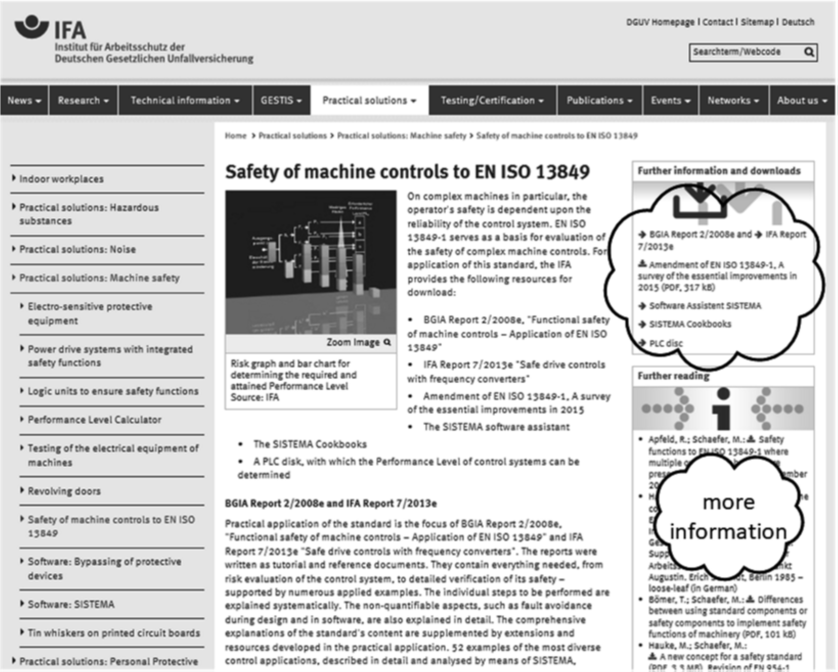
\includegraphics[width=0.8\textwidth]{img02-01.png}
    \caption{Questo sito web fornisce i link a tutti gli strumenti pratici riguardanti la sicurezza dei comandi delle macchine}
    \label{fig:02-01}
\end{figure}




%==============================================================
%  CAPITOLO 3
%==============================================================
\chapter{Norme generali sulla sicurezza funzionale delle macchine}
\label{cap:03}

Oltre alla norma EN ISO 13849, di cui si discute in questo rapporto, esistono norme generiche alternative di rilevanza nel campo della sicurezza funzionale. Come mostrato nella Figura~\ref{fig:03-01}, queste norme sono quelle della serie IEC 61508~\cite{iec61508} e la relativa norma di settore IEC 62061~\cite{iec62061} per l'industria meccanica. Entrambe sono limitate nel loro ambito ai sistemi elettrici, elettronici ed elettronici programmabili.
\begin{figure}[ht]
    \centering
    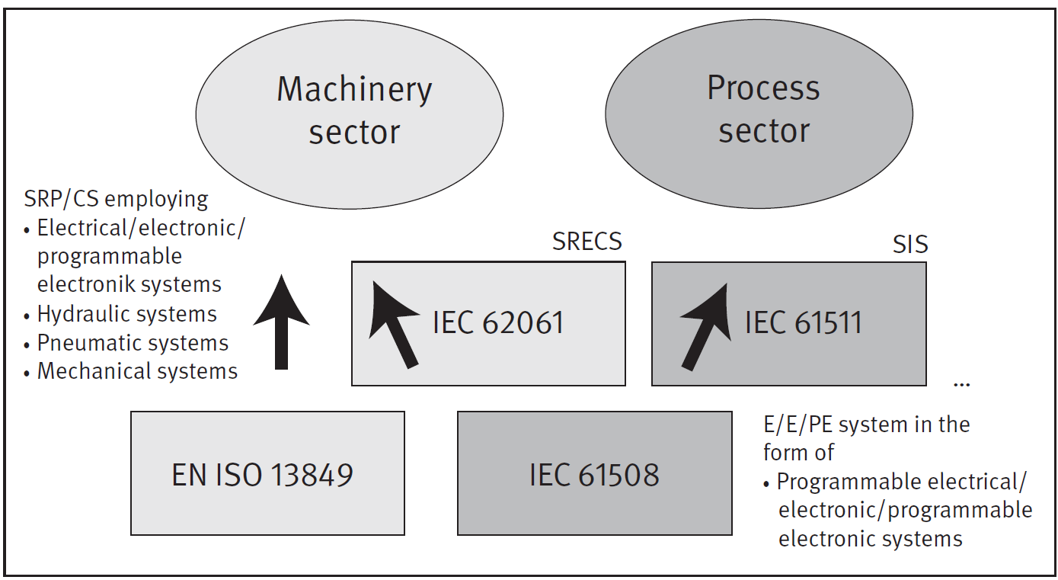
\includegraphics[width=0.8\textwidth]{img03-01.png}
    \caption{Campo di applicazione delle norme generiche che disciplinano la sicurezza funzionale; SRP/CS: parte di un sistema di comando legata alla sicurezza; SRECS: sistema di comando elettrico legato alla sicurezza; SIS: sistema strumentato di sicurezza; sistema E/E/PE: sistema elettrico/elettronico/elettronico programmabile.}
    \label{fig:03-01}
\end{figure}

Un sistema di classificazione che prevede i “Livelli di Integrità di Sicurezza” (SIL) è definito nelle norme IEC 61508 e IEC 62061. I SIL fungono da indicatori del livello di affidabilità in relazione alla sicurezza. I valori associati rappresentano misure di guasto obiettivo, ciascuna comprendente un decennio. La norma IEC 61508 distingue due diverse applicazioni delle funzioni di sicurezza:
\begin{itemize}
    \item funzioni di sicurezza in modalità a bassa richiesta (frequenza massima delle richieste una volta all'anno)
    \item funzioni di sicurezza in modalità ad alta richiesta o continua
\end{itemize}
In modalità a bassa richiesta, la dimensione per la sicurezza è la probabilità media di un guasto pericoloso di una funzione di sicurezza nel momento della richiesta: PFDavg. In modalità ad alta richiesta o continua, la probabilità media di un guasto pericoloso per ora PFH\textsubscript{D} è valutata dalla norma IEC 62061 (per ulteriori informazioni, fare riferimento anche a~\cite{boemer2014}). Con alcune eccezioni, solo la seconda definizione è rilevante nel settore dei macchinari e quindi nella norma IEC 62061. La nuova edizione della norma EN ISO 13849-1 ha adottato anche questa definizione della modalità operativa e limita di conseguenza l'ambito di applicazione della norma. I sistemi SIL 4 con rischi più elevati non sono noti nel settore dei macchinari e non sono quindi considerati nella norma IEC 62061.
\begin{figure}[ht]
    \centering
    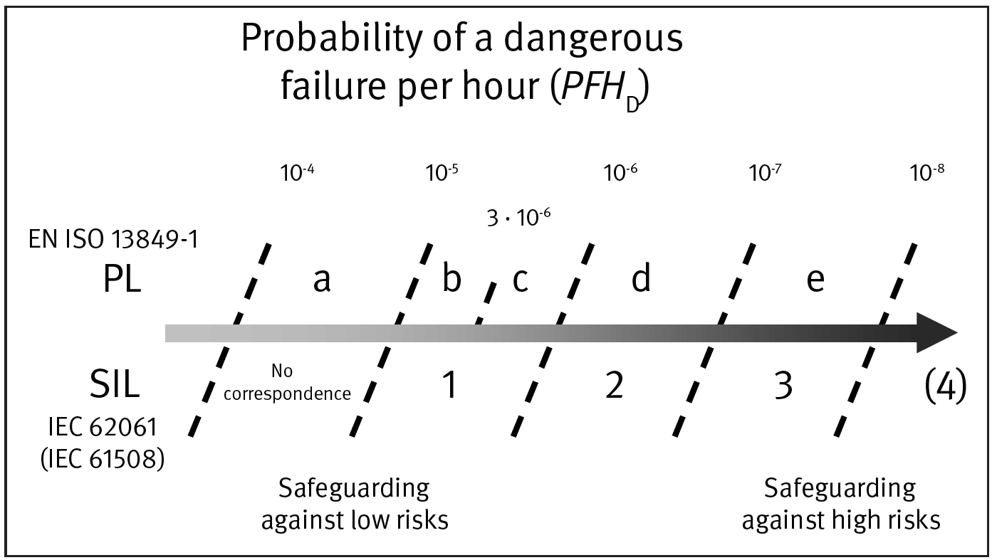
\includegraphics[width=0.8\textwidth]{img03-02.png}
    \caption{Questo sito web fornisce i link a tutti gli strumenti pratici riguardanti la sicurezza dei comandi delle macchine}
    \label{fig:03-02}
\end{figure}
L'approccio essenziale delle norme che regolano la sicurezza funzionale (IEC 61508 e IEC 62061) sviluppate dalla Commissione Elettrotecnica Internazionale (IEC), ovvero quello di definire le probabilità di guasto come parametro caratteristico senza l'inclusione specifica delle architetture, appare inizialmente più universale. L'approccio della norma EN ISO 13849-1, tuttavia, offre agli utenti la possibilità di sviluppare e valutare funzioni di sicurezza, da un sensore a un attuatore (ad esempio una valvola), nell'ambito di un'unica norma, anche se le funzioni possono coinvolgere tecnologie diverse. La Parte 1 della norma EN ISO 13849 è accompagnata da una Parte 2 intitolata "Validazione".

La presente edizione, pubblicata nel 2012, prende in considerazione anche l'attuale.

Gli allegati da A a D della Parte 2 contengono materiale esaustivo sui temi dei "principi di sicurezza di base", dei "principi di sicurezza collaudati", dei "componenti collaudati" e degli "elenchi dei guasti". Ulteriori dettagli sono reperibili nell'allegato C della presente relazione.

L'apparente sovrapposizione nell'ambito normativo delle due sfere di standardizzazione appare inizialmente sfavorevole ai produttori di sistemi di controllo e agli altri utilizzatori delle norme. Sia la norma EN ISO 13849-1 che la IEC 62061 sono norme armonizzate ai sensi della Direttiva Macchine.

Le parti da 1 a 4 della norma IEC 61508 hanno lo status di norme di sicurezza di base dal punto di vista IEC (con l'eccezione dei sistemi semplici); questa serie di norme non può tuttavia essere armonizzata ai sensi della Direttiva Macchine, nemmeno come norma europea. Questa situazione solleva, ad esempio, le seguenti domande:
\begin{itemize}
    \item Quali standard dovrebbero essere applicati per la conformità con la Direttiva Macchine?
    \item Laddove si sovrappongono nel loro ambito, producono risultati equivalenti?
    \item Sono i sistemi di classificazione degli standard, come ad esempio Categorie, Performance Level (PL) e Integrità della Sicurezza Livello (SIL), compatibile?
    \item È possibile utilizzare dispositivi sviluppati in conformità a una delle due norme durante l'implementazione di una funzione di sicurezza secondo una norma diversa?
\end{itemize}
Per raggiungere la massima compatibilità possibile con la IEC, e se possibile per consentire la fusione a lungo termine delle due sfere di standardizzazione e anche per permettere di sfruttare i vantaggi dell'approccio probabilistico senza abbandonare le categorie collaudate, la norma EN ISO 13849-1, in quanto successore della EN 954-1, tenta di trovare un equilibrio tra l'approccio deterministico delle categorie e l'aspetto dell'affidabilità della sicurezza con la definizione del livello di prestazione (PL) (vedere anche~\cite{hauke2006}). Numericamente, esistono classi corrispondenti (vedere Figura~\ref{fig:03-02}) che consentono rapide stime preliminari per l'uso pratico quotidiano.

Nel senso della norma, le architetture designate sono più una funzionalità opzionale (approccio semplificato) che un requisito. Devono tuttavia essere considerate un elemento chiave nella semplificazione dell'approccio probabilistico implementato nella norma EN ISO 13849, e la loro applicazione è uno dei principi cardine di questo rapporto. L'ambito di applicazione della norma IEC 62061 indica che essa copre anche l'elettronica complessa, ad esempio quella programmabile. Sebbene ciò sia corretto, lo sviluppo di "SRECS" (vedere Figura~\ref{fig:03-01}) che impiegano questa tecnologia deve comunque soddisfare i requisiti della norma in conformità con la norma IEC 61508. L'ambito di applicazione degli SRP/CS sviluppati secondo le norme derivate dalla IEC è sottolineato dalla nuova edizione della norma EN ISO 13849-1. Ciò significa che tali SRP/CS possono essere considerati ugualmente validi quando utilizzati per l'implementazione di funzioni di sicurezza ai sensi della norma EN ISO 13849-1.

Gli argomenti decisivi dal punto di vista degli utenti del settore per la scelta della norma EN ISO 13849 come base per l'implementazione della sicurezza funzionale nel settore dei macchinari possono essere considerati l'approccio interdisciplinare in termini di tecnologia e l'approccio semplificato alla quantificazione con l'uso delle architetture designate. Ciò include la considerazione dettagliata dei componenti non elettrici ed elettromeccanici. I produttori di grandi volumi di un componente di sicurezza, come un controllore logico programmabile (PLC) per applicazioni di sicurezza, ovviamente desidereranno servire in particolare altri mercati mondiali oltre a quello dei macchinari e baseranno quindi la loro attività di sviluppo sulla norma IEC 61508 oltre che sulla EN ISO 13849.

La tabella precedente presente in forma identica nelle introduzioni di EN ISO 13849-1 e IEC 62061 per la selezione dello standard appropriato per l'applicazione pertinente è stata ora eliminata da entrambi gli standard. Esiste un documento guida sull'applicazione di EN ISO 13849-1 e IEC 62061 durante la progettazione di controlli di sicurezza per macchine, sebbene abbia ricevuto poca attenzione. Essendo uno standard di settore di IEC 61508, IEC 62061 descrive naturalmente in modo molto esplicito l'aspetto della "gestione della sicurezza funzionale". Lo sviluppo e la verifica del software embedded secondo EN ISO 13849-1 si basano sui requisiti essenziali per il software relativo alla sicurezza che sono attualmente prassi standard e sono descritti anche in IEC 61508. Esiste tuttavia un ampio consenso sul fatto che i requisiti dei due standard non debbano essere mescolati. Il documento guida ISO/TR 23849~\cite{isotr23849} è stato sviluppato dai membri di entrambi i comitati di normazione ed è stato pubblicato nel 2010 da ISO e IEC. I suoi messaggi principali sono:
\begin{itemize}
    \item I metodi descritti dalle due normative differiscono, ma possono raggiungere un livello comparabile di riduzione del rischio.
    \item Le attività che integrano i due standard richiedono un'adeguata esperienza nella loro applicazione pratica.
\end{itemize}
Già nel 2011 la IEC propose la fusione dei due standard per formare uno standard ISO/IEC, e avviò i lavori nel 2012. I risultati di un'indagine internazionale condotta durante i lavori sulla norma ISO/IEC 17305 mostrarono chiaramente che gli standard 13849 erano predominanti nell'applicazione tra i produttori di macchine e gli utenti finali. Come mostrato nella Figura~\ref{fig:03-03}, la norma EN ISO 13849-1 era utilizzata dal 90\%, ovvero dalla grande maggioranza delle 715 persone intervistate. Lo sviluppo del previsto standard ISO/IEC 17305 fu oggetto di accese discussioni tra gli esperti. Le lunghe discussioni avevano portato il progetto ad accumulare almeno due anni di ritardo rispetto alla tabella di marcia originale. Il gruppo di lavoro era già consapevole dell'essenziale necessità di considerare la compatibilità con le norme EN ISO 13849-1 e IEC 62061. 

L'applicazione diretta del nuovo standard e il mantenimento dei metodi esistenti erano obiettivi espliciti. Non è possibile rispondere alla domanda se un nuovo standard avrebbe raggiunto questi obiettivi e se sarebbe stato in grado di sostituire gli standard esistenti. Nell'ottobre 2015, l'ISO/TC 199 ha deciso di abbandonare i lavori su uno standard comune e di sospendere le attività del gruppo di lavoro. Tuttavia, non appena i lavori si sono ufficialmente interrotti, è apparso chiaro che la questione non sarebbe stata risolta. Pertanto, si dovranno formulare raccomandazioni se e, in caso affermativo, come, un futuro progetto comune sulla sicurezza funzionale potrebbe essere condotto congiuntamente dai due organismi di normazione. Entrambi gli standard saranno rivisti a breve nell'ambito della "manutenzione ordinaria". I risultati del lavoro svolto finora sulla norma ISO/IEC 17305 saranno recepiti in entrambi gli standard.
\begin{figure}[ht]
    \centering
    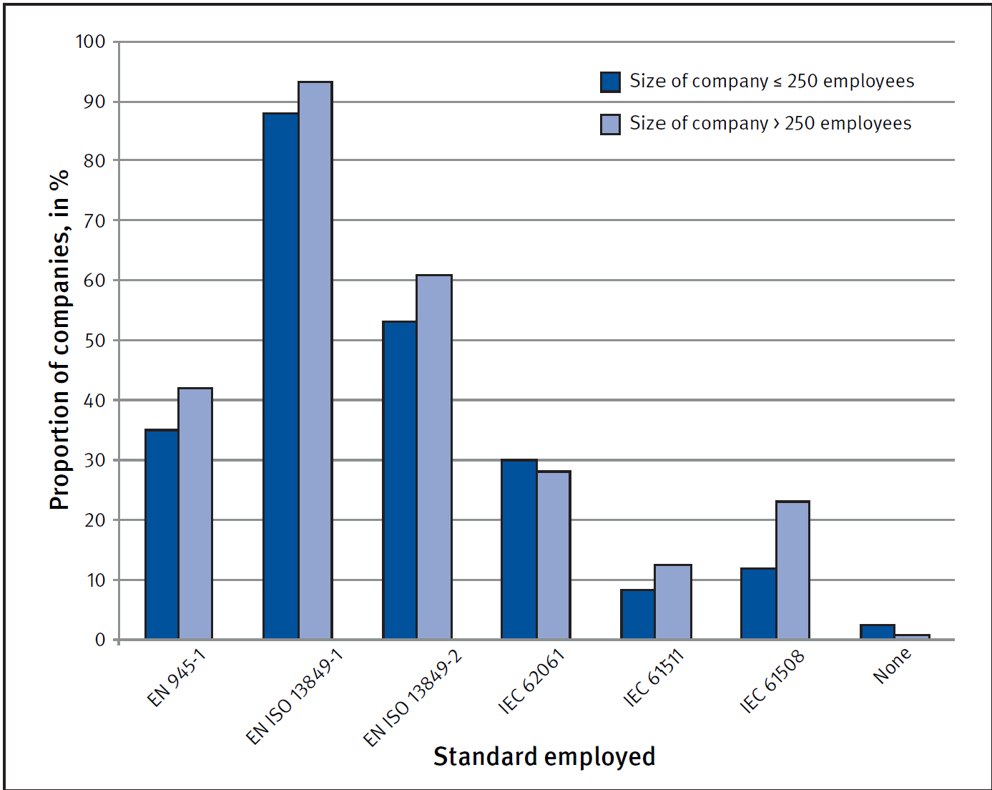
\includegraphics[width=0.8\textwidth]{img03-03.png}
    \caption{Norme utilizzate dai fabbricanti di macchine e dagli utilizzatori finali, secondo quanto emerso da un'indagine condotta nel 2012/2013 da ISO e IEC in vista della fusione della EN ISO 13849-1 e della IEC 62061.}
    \label{fig:03-03}
\end{figure}

%==============================================================
%  CAPITOLO 4
%==============================================================
\chapter{Rapporto e standard: una panoramica}
\label{cap:04}

Questo capitolo rimanda ai capitoli successivi e agli allegati di questa relazione relativi alla norma. Allo stesso tempo, fornisce una panoramica del processo iterativo per la progettazione delle parti relative alla sicurezza dei sistemi di controllo, basandosi sulla Figura 4.1, che corrisponde alla Figura 3 della norma. Le modifiche tra la seconda e la terza edizione della norma, e il suo sviluppo futuro, sono discusse alla fine del capitolo.

% La minipage tiene insieme disegno e didascalia (figura non fluttuante)
\begin{center}
    \begin{minipage}{\textwidth}
        \centering
        \captionsetup{hypcap=false}
        \resizebox{!}{0.72\textheight}{%==============================================================
%  Figura 4.1 - Processo iterativo per la progettazione delle
%  parti dei sistemi di comando legate alla sicurezza (SRP/CS)
%  Adattamento in italiano della Figura 4.1 dell'IFA Report 2/2017
%  (e' il processo completo di cui le Figure 5.5, 6.1 e 7.1 sono
%  estratti: stesso stile e stessa terminologia)
%
%  I riquadri sono piu' larghi che nell'originale perche' il testo
%  italiano e' piu' lungo di quello inglese.
%==============================================================
\begin{tikzpicture}[
  font=\normalsize,
  grigio/.style={fill=black!10, align=center, inner sep=4pt},
  numcella/.style={draw=black, fill=white, line width=0.8pt,
                   minimum width=0.7cm, minimum height=0.75cm, inner sep=1pt},
  corpo/.style={draw=black, fill=black!10, line width=0.8pt, align=center,
                minimum width=10.2cm, text width=9.8cm, minimum height=0.75cm,
                inner sep=3pt},
  decis/.style={diamond, draw=black, fill=black!10, line width=0.8pt,
                align=center, inner sep=1pt, aspect=4.0, minimum width=10.0cm},
  fdline/.style={draw=black, line width=0.9pt},
  fdar/.style={fdline, -{Triangle[length=6pt,width=6pt]}}
]

%--------------------------------------------------------------
% Ingresso e uscita verso l'analisi dei rischi
%--------------------------------------------------------------
\node[grigio, minimum width=4.45cm, minimum height=1.3cm, anchor=east]
  (entrata) at (4.0,-0.65) {Dall'analisi dei rischi\\ (EN ISO 12100)};
\node[grigio, minimum width=4.45cm, minimum height=1.3cm, anchor=east]
  (uscita) at (4.0,-20.60) {All'analisi dei rischi\\ (EN ISO 12100)};

%--------------------------------------------------------------
% Fasi da 1 a 4
%--------------------------------------------------------------
\foreach \n/\y/\testo in {%
  1/-2.01/{Identificazione delle funzioni di sicurezza (SF)},
  2/-3.27/{Specifica delle caratteristiche di ciascuna SF},
  3/-4.52/{Determinazione del PL richiesto (PL\textsubscript{r})},
  4/-6.31/{Realizzazione delle SF, identificazione degli SRP/CS}}{
  \node[numcella, anchor=west] (num\n) at (3.3,\y) {\n};
  \node[corpo, anchor=west] (fase\n) at (4.0,\y) {\testo};
}

%--------------------------------------------------------------
% Fase 5: valutazione del PL, su due riquadri
%--------------------------------------------------------------
\node[corpo, minimum height=1.30cm, anchor=west] (fase5a) at (4.0,-7.94)
  {Valutazione del PL degli SRP/CS in termini di categoria,
   \textit{MTTF}\textsubscript{D}, \textit{DC}\textsubscript{avg}, CCF};
\node[corpo, anchor=west] (fase5b) at (4.0,-9.025) {Software e guasti sistematici};
\node[numcella, minimum height=2.11cm, anchor=west] (num5) at (3.3,-8.345) {5};

%--------------------------------------------------------------
% Fasi 6, 7 e 8: verifica, validazione e completezza dell'analisi
%--------------------------------------------------------------
\node[decis] (dec6) at (9.1,-11.43) {Verifica:\\[2pt] PL $\geq$ PL\textsubscript{r}?};
\node[decis] (dec7) at (9.1,-14.82) {Validazione:\\[2pt] requisiti soddisfatti?};
\node[decis] (dec8) at (9.1,-18.25) {Tutte le SF\\[2pt] analizzate?};

\node[numcella, anchor=west] at (3.3,-11.43) {6};
\node[numcella, anchor=west] at (3.3,-14.82) {7};
\node[numcella, anchor=west] at (3.3,-18.25) {8};

%--------------------------------------------------------------
% Percorso principale
%--------------------------------------------------------------
\draw[fdar] (4.0,-0.65) -- (9.1,-0.65) -- (9.1,-1.635);
\draw[fdar] (9.1,-2.385) -- (9.1,-2.895);
\draw[fdar] (9.1,-3.645) -- (9.1,-4.145);
\draw[fdar] (9.1,-4.895) -- (9.1,-5.22);
\draw[fdline] (9.1,-5.37) circle (0.15);
\draw[fdar] (9.1,-5.52) -- (9.1,-5.935);
\draw[fdar] (9.1,-6.685) -- (9.1,-7.29);
\draw[fdar] (9.1,-9.40) -- (9.1,-10.18);
\draw[fdar] (9.1,-12.68) -- (9.1,-13.57);
\draw[fdar] (9.1,-16.07) -- (9.1,-17.00);
\draw[fdline] (9.1,-19.50) -- (9.1,-20.60);
\draw[fdar] (9.1,-20.60) -- (4.0,-20.60);

\node[anchor=east] at (9.00,-13.12) {s\`i};
\node[anchor=east] at (9.00,-16.53) {s\`i};
\node[anchor=east] at (9.00,-20.05) {s\`i};

%--------------------------------------------------------------
% "Per ciascuna SF" con graffa
%--------------------------------------------------------------
\node[grigio, minimum width=1.5cm, minimum height=1.9cm] (perogni) at (1.20,-10.21)
  {Per\\ ciascuna\\ SF};
\draw[fdline, decorate, decoration={brace, amplitude=6pt}] (2.80,-16.35) -- (2.80,-3.98);

%--------------------------------------------------------------
% Rami "no": ritorno alla realizzazione (6 e 7) e alla SF
% successiva (8)
%--------------------------------------------------------------
\draw[fdar] (dec6.east) -- (15.30,-11.43);
\draw[fdar] (dec7.east) -- (15.30,-14.82);
\draw[fdline] (15.30,-14.82) -- (15.30,-5.37);
\draw[fdar] (15.30,-5.37) -- (9.25,-5.37);

\draw[fdar] (dec8.east) -- (16.20,-18.25);
\draw[fdline] (16.20,-18.25) -- (16.20,-3.27);
\draw[fdar] (16.20,-3.27) -- (14.20,-3.27);

\node[anchor=south west] at (14.25,-11.40) {no};
\node[anchor=south west] at (14.25,-14.79) {no};
\node[anchor=south west] at (14.25,-18.22) {no};

%--------------------------------------------------------------
% Cornice
%--------------------------------------------------------------
\draw[draw=black, line width=1pt]
  ([shift={(-0.45,0.45)}]current bounding box.north west) rectangle
  ([shift={(0.45,-0.45)}]current bounding box.south east);

\end{tikzpicture}
}
        \captionof{figure}{Processo iterativo per la progettazione delle parti dei sistemi di comando legate alla sicurezza: SF = funzione di sicurezza; PL = livello di prestazione; PL\textsubscript{r} = livello di prestazione richiesto; SRP/CS = parte di un sistema di comando legata alla sicurezza; \textit{MTTF}\textsubscript{D} = tempo medio al guasto pericoloso; \textit{DC}\textsubscript{avg} = copertura diagnostica media; CCF = guasto di causa comune.}
        \label{fig:04-01}
    \end{minipage}
\end{center}

%--------------------------------------------------------------
\section{Identificazione delle funzioni di sicurezza e delle loro proprietà}
\label{sec:04-1}

Il processo di progettazione e valutazione inizia con un concetto consolidato, ovvero la definizione di una o più funzioni di sicurezza (FS). La procedura è illustrata nella Figura 4.1 dai blocchi da 1 a 3 ed è descritta in modo più dettagliato nel Capitolo~\ref{cap:05}. La domanda a cui si deve rispondere è: in che modo le parti del sistema di controllo relative alla sicurezza contribuiscono a ridurre il rischio di un pericolo su una macchina?

In primo luogo, una macchina deve essere costruita in modo tale da non presentare più alcun pericolo durante l'uso (sicurezza intrinseca). Il secondo passo consiste quindi nel ridurre il rischio di qualsiasi pericolo che possa ancora presentarsi. Ciò può essere ottenuto mediante misure di protezione, che spesso comprendono una combinazione di dispositivi di protezione e controllo di sicurezza.

Affinché tali misure di protezione raggiungano una qualità definita in relazione al rischio, un passaggio essenziale è la valutazione del rischio, come richiesto dalla Direttiva Macchine e descritto nella norma EN ISO 12100~\cite{eniso12100}. I dispositivi di protezione sono considerati, ai sensi della norma EN ISO 13849-1 (dispositivi di sicurezza), insieme al controllo di sicurezza, come la parte relativa alla sicurezza di un sistema di controllo. Insieme, svolgono una funzione di sicurezza; possono ad esempio impedire l'avvio imprevisto quando un operatore entra in una zona di pericolo. Poiché una macchina può facilmente avere diverse funzioni di sicurezza (ad esempio per le modalità automatiche e di impostazione), è importante valutare attentamente ogni singolo pericolo e la relativa funzione di sicurezza.

La funzione di sicurezza può essere assunta da parti del sistema di controllo della macchina o da componenti richiesti in aggiunta ad esso. In entrambi i casi, queste parti sono componenti di sicurezza dei sistemi di controllo. Sebbene lo stesso hardware possa essere coinvolto nell'esecuzione di diverse funzioni di sicurezza, la qualità richiesta della riduzione del rischio per ciascuna funzione di sicurezza può variare. Nella norma, la qualità della riduzione del rischio è definita dal termine "Livello di Prestazione" (PL). Il risultato della valutazione del rischio determina il livello del valore PL richiesto per la funzione di sicurezza. Questa specifica per la progettazione del sistema di controllo è descritta come "Livello di Prestazione richiesto", PL\textsubscript{\small r}. Come si ottiene il PL?

Il rischio di un pericolo su una macchina può essere ridotto non solo dal sistema di controllo, ma anche, ad esempio, da una protezione, come un cancello di protezione, o da dispositivi di protezione individuale, come gli occhiali di sicurezza. Una volta stabilito il ruolo delle misure di protezione fornite dal sistema di controllo, il livello di prestazione richiesto (PL\textsubscript{\small r}) viene determinato in modo rapido e diretto con l'ausilio di un semplice albero decisionale, il "grafico del rischio". La lesione associata è irreversibile (ad esempio, morte, perdita di arti) o reversibile (ad esempio, lesioni da schiacciamento, che possono guarire)? L'operatore è presente nella zona di pericolo frequentemente e per lunghi periodi (ad esempio, più frequentemente di una volta ogni quindici minuti) o raramente e per brevi periodi? L'operatore è ancora in grado di evitare un incidente (ad esempio, grazie a movimenti lenti della macchina)?
Queste tre domande determinano il PL\textsubscript{\small r}. Ulteriori dettagli sono disponibili nella sotto clausola~\ref{sec:05-4}, esempi nell'Allegato~\ref{app:A}.

%--------------------------------------------------------------
\section{Progettazione e implementazione tecnica delle funzioni di sicurezza}
\label{sec:04-2}
Una volta definiti i requisiti relativi alle parti dei sistemi di controllo che riguardano la sicurezza, questi vengono prima progettati e poi implementati. Infine, viene effettuata una verifica per accertare se la riduzione del rischio richiesta, ovvero il valore PL\textsubscript{\small r} target (blocco 6 nella Figura 4.1), possa essere raggiunta mediante l'implementazione pianificata (blocchi 4 e 5 nella Figura 4.1) con il valore PL effettivo.

Le fasi dei blocchi 4 e 5 sono descritte in dettaglio nel Capitolo~\ref{cap:06}. Seguendo la tradizione dei precedenti rapporti sui sistemi di controllo, anche il Capitolo~\ref{cap:08} di questo rapporto contiene un gran numero di esempi di circuiti per tutte le tecnologie di controllo e per ciascuna Categoria. Inoltre, le descrizioni generali contenute nei Capitoli~\ref{cap:05}, \ref{cap:06} e~\ref{cap:07} sono accompagnate da una descrizione completa di un esempio di circuito (una ghigliottina per il taglio della carta). Ciò fornisce allo sviluppatore una spiegazione illustrativa dei metodi e dei parametri descritti di seguito.

Le componenti di sicurezza dei sistemi di controllo possono esercitare il loro effetto di riduzione del rischio solo se la funzione di sicurezza è stata definita correttamente fin dall'inizio. Durante la successiva implementazione, vengono applicati criteri di qualità quali la qualità dei componenti impiegati (durata di vita), la loro interazione (dimensionamento), l'efficacia della diagnostica (ad esempio, autodiagnosi) e la tolleranza ai guasti della struttura. Questi parametri determinano la probabilità media di un guasto pericoloso per ora (PFH\textsubscript{D}) e quindi il livello di sicurezza (PL) raggiunto. La norma EN ISO 13849-1 lascia a discrezione dell'utente i metodi con cui viene calcolato il PL. Pertanto, è possibile utilizzare anche il metodo di modellazione di Markov, molto complesso, nel rispetto dei parametri sopra indicati. La norma, tuttavia, descrive una procedura molto semplificata, ovvero l'utilizzo di architetture designate con l'applicazione di un diagramma a barre (vedere Figura 6.10), in cui la modellazione del PL è già inclusa.
Gli esperti interessati alla derivazione del diagramma a barre possono trovarla nell'Allegato G.

Le Categorie continuano a essere la base su cui viene determinato il PL. La loro definizione rimane sostanzialmente invariata rispetto alla prima edizione della norma; a partire dalla seconda edizione, tuttavia, sono stati introdotti requisiti aggiuntivi relativi alla qualità dei componenti e all'efficacia della diagnostica. Per le Categorie 2, 3 e 4 sono inoltre richieste misure adeguate contro il guasto di causa comune (Tabella~\ref{tab:04-1}).

\begin{table}[ht]
    \centering
    \footnotesize
    \setlength{\tabcolsep}{4pt}
    \caption{Caratteristiche deterministiche e probabilistiche delle categorie; le aggiunte probabilistiche introdotte a partire dalla seconda edizione della norma sono evidenziate in grigio.}
    \label{tab:04-1}
    \begin{tabularx}{\textwidth}{|p{6cm}|*{5}{C|}}
        \hline
        \multirow{2}{*}{\textbf{Funzionalità}} & \multicolumn{5}{c|}{\textbf{Categoria}} \\
        \cline{2-6}
        & \textbf{B} & \textbf{1} & \textbf{2} & \textbf{3} & \textbf{4} \\
        \hline
        Progettazione conformemente alle norme pertinenti; resistenza alle influenze previste & X & X & X & X & X \\
        \hline
        Principi di sicurezza base & X & X & X & X & X \\
        \hline
        Principi di sicurezza ben collaudati & & X & X & X & X \\
        \hline
        Componenti ben collaudati & & X & & & \\
        \hline
        \rowcolor{black!10}
        Tempo medio guasto pericoloso -- MTTF\textsubscript{D} & Da basso a medio & Alto & Da basso a alto & Da basso a alto & Alto \\
        \hline
        Rilevazione dei guasti (test) & & & X & X & X \\
        \hline
        Tolleranza al guasto singolo & & & & X & X \\
        \hline
        Considerazione accumulo guasti & & & & & \\
        \hline
        \rowcolor{black!10}
        Copertura diagnostica media -- DC\textsubscript{avg} & Nessuno & Nessuno & Da basso a medio & Da basso a medio & Alto \\
        \hline
        Caratterizzata principalmente da & \multicolumn{2}{c|}{Selezione dei componenti} & \multicolumn{3}{c|}{Struttura} \\
        \hline
    \end{tabularx}
\end{table}

La Tabella 6.2 fornisce una sintesi delle Categorie. Un aspetto essenziale, quando si utilizza il metodo di calcolo semplificato proposto, è la rappresentazione delle Categorie come diagrammi a blocchi logici, denominati "architetture designate".

Poiché le Categorie richiedono l'analisi dei guasti (evitamento e controllo dei guasti), aspetti aggiuntivi riguardano l'affidabilità dei singoli componenti, i loro modi di guasto e il rilevamento dei guasti mediante misure diagnostiche automatiche. Le liste dei guasti e i principi di sicurezza fungono qui da base (vedi Allegato~\ref{app:C}). Oltre alla tradizionale FMEA (analisi dei modi di guasto e dei loro effetti), la EN ISO 13849-1 offre metodi di calcolo semplificati, come il metodo del conteggio dei componenti (parts count method). Ulteriori approfondimenti su questo argomento sono riportati nell'Allegato~\ref{app:B}.

Una delle domande più frequenti riguardo alla probabilità di guasto riguarda il reperimento di dati di guasto affidabili per i componenti legati alla sicurezza, ovvero i valori di MTTF\textsubscript{D} (tempo medio al guasto pericoloso). A tale scopo, la fonte da privilegiare rispetto a tutte le altre è il costruttore dei componenti, ossia la sua scheda tecnica. Molti costruttori di componenti forniscono già questo tipo di dati. Anche laddove i dati del costruttore non siano disponibili, tuttavia, valori tipici di esempio possono essere ricavati da banche dati consolidate (come SN 29500 o IEC/TR 62380). La norma e l'Allegato~\ref{app:D} del presente report elencano inoltre una serie di valori realistici ricavati dal campo, e forniscono indicazioni sulla modellazione nello schema a blocchi legato alla sicurezza.

L'efficacia della diagnostica, espressa dal valore DC\textsubscript{avg} (copertura diagnostica media), può essere determinata secondo il seguente principio semplice: per ciascun blocco vengono raccolte le misure di test che lo sorvegliano.

Per ciascuna di queste misure di test, si determina uno dei quattro valori tipici di DC a partire da una tabella riportata nella norma. Da questi valori si può calcolare il parametro DC\textsubscript{avg} mediante una formula di media che appare complessa ma è in realtà semplice. Ulteriori informazioni sono disponibili al paragrafo~\ref{subsec:06-2-14} e nell'Allegato E.

L'ultimo parametro, quello del CCF (guasto di causa comune, paragrafo 6.2.15), è altrettanto facile da calcolare: per questo parametro si presume che una causa, come contaminazione, sovratemperatura o cortocircuito, possa in determinate circostanze dare origine a più guasti che possono ad esempio disabilitare simultaneamente entrambi i canali di controllo. Per il controllo di questa fonte di pericolo, per i sistemi di Categoria 2, 3 e 4 occorre dimostrare che sono state adottate misure adeguate contro il CCF. Ciò si ottiene mediante un sistema a punti riferito a otto contromisure tipiche, per lo più di natura tecnica, con il quale è necessario raggiungere almeno 65 dei 100 punti disponibili (per i dettagli, vedi Allegato F).

Ai guasti hardware casuali, che possono essere controllati mediante una buona struttura e una bassa probabilità di guasto, si affianca il vasto ambito dei guasti sistematici - ossia guasti insiti nel sistema fin dalla sua progettazione, come errori di dimensionamento, guasti software o errori logici - contro i quali occorre garantire protezione mediante misure di evitamento e controllo dei guasti. I guasti software costituiscono una parte rilevante di questi guasti. Fin dalla sua seconda edizione, la norma include i requisiti relativi al software legato alla sicurezza; alcuni aspetti specifici di questi requisiti erano tuttavia già noti da tempo dalle norme pertinenti. Le misure effettive sono graduate in funzione del PL richiesto. Ulteriori informazioni sono disponibili al paragrafo~\ref{subsec:06-1-2} per i guasti sistematici e al paragrafo 6.3 per il software.

\section{Verifica e validazione del sistema di comando per ciascuna funzione di sicurezza}
\label{sec:04-3}
Se la progettazione ha già raggiunto una fase avanzata nel momento in cui viene determinato il PL raggiunto, si pone la questione se tale PL sia sufficiente per ciascuna funzione di sicurezza eseguita dal sistema di comando. A tale scopo, il PL viene confrontato con il PL\textsubscript{\small r} richiesto (vedi Blocco 6, Figura 4.1). Se il PL raggiunto per una funzione di sicurezza è inferiore al PL\textsubscript{\small r} richiesto, sono necessari miglioramenti progettuali di entità maggiore o minore (come l'impiego di componenti alternativi con un MTTF\textsubscript{D} superiore), fino a raggiungere infine un PL adeguato. Superato questo ostacolo, è necessaria una serie di fasi di validazione. A questo punto entra in gioco la Parte 2 della EN ISO 13849. Questo processo di validazione assicura in modo sistematico che tutti i requisiti funzionali e prestazionali posti alle parti dei sistemi di comando legate alla sicurezza siano stati soddisfatti (vedi Blocco 7, Figura 4.1). Ulteriori dettagli sono riportati nel Capitolo~\ref{cap:07}.

\section{Modifiche derivanti dalla terza edizione della norma pubblicata nel 2015}
\label{sec:04-4}
Con l'Emendamento 1, dalla seconda edizione è stata prodotta la terza edizione della norma. I passaggi modificati servono principalmente a migliorare la comprensibilità e l'applicazione. Una panoramica dettagliata incentrata sulle modifiche è stata pubblicata dall'IFA nel 2015~\cite{hauke2015}. Le modifiche essenziali comprendono la considerazione, in fase di specifica del Performance Level richiesto (PL\textsubscript{\small r}), della probabilità di accadimento di un evento pericoloso; un nuovo metodo semplificato per la determinazione del PL della parte di uscita della parte del sistema di comando legata alla sicurezza (SRP/CS); e una proposta per la gestione dei requisiti relativi al SRESW (software embedded legato alla sicurezza) quando vengono utilizzati componenti standard. La Tabella~\ref{tab:04-2} mostra in quali paragrafi della norma e del presente report sono state apportate le principali modifiche.

Gli schemi circuitali degli esempi riportati nel Capitolo~\ref{cap:08} del report sono stati completamente aggiornati rispetto alle versioni del 2008, sulla base delle suddette modifiche alla norma.

\section{Sviluppi futuri della EN ISO 13849-1}
\label{sec:04-5}
La terza edizione della EN ISO 13849-1 sostituisce l'edizione precedente senza un periodo di transizione specifico. Poiché le modifiche - come descritto nel paragrafo precedente - riguardano essenzialmente integrazioni, aggiornamenti e miglioramenti, il passaggio dalla seconda alla terza edizione della norma non è tuttavia generalmente critico. Come già avviene da tempo, l'IFA sostiene questo processo con guide applicative liberamente disponibili. Queste guide si presentano sia sotto forma di riferimenti esplicativi con esempi, sia come il programma software gratuito "SISTEMA" (l'acronimo sta per "Safety Integrity Software Tool for the Evaluation of Machine Applications"), che supporta il calcolo e la documentazione del PL\textsubscript{\small r} e del PL (vedi Allegato H). La serie dei ricettari SISTEMA (SISTEMA cookbooks), costantemente ampliata, è dedicata a temi specifici rilevanti nell'applicazione della norma. Questi riguardano non solo SISTEMA stesso (le librerie SISTEMA, l'uso delle librerie di rete, "l'esecuzione di più istanze di SISTEMA in parallelo"), ma anche l'intero processo di progettazione secondo la norma ("Definizione delle funzioni di sicurezza", "Dallo schema elettrico al Performance Level", "Quando le architetture designate non corrispondono"). Infine, tra le risorse rientra il "Performance Level Calculator"~\cite{schaefer2015plc} sviluppato dall'IFA. Questo presenta il diagramma a barre sotto forma di disco rotante, mediante il quale è possibile determinare in modo semplice e preciso, in qualsiasi momento, il PFH\textsubscript{D} e il PL. Tutte le ulteriori risorse e riferimenti - come le informazioni sulle norme di prova e sui principi~\cite{dguvtest} di DGUV Test, il sistema di prova e certificazione dell'Assicurazione Sociale Tedesca contro gli Infortuni - sono disponibili sul sito web dell'IFA: www.dguv.de/ifa/13849.

Nel corso dei lavori sulla terza edizione della EN ISO 13849-1, sono stati individuati diversi pacchetti di lavoro rilevanti che esulavano dall'ambito di un semplice emendamento. Tra questi, ad esempio, una revisione approfondita dei requisiti relativi al software, al fine di migliorarne l'idoneità all'applicazione pratica, nonché una precisazione coerente di quando il termine "SRP/CS" si riferisca all'intero sistema di comando che esegue una funzione di sicurezza, e quando invece a un sottosistema che esegue solo una parte della funzione di sicurezza. Affinché queste proposte potessero essere attuate nel lungo termine, il comitato responsabile della norma ha deciso già nel 2016, subito dopo la pubblicazione della terza edizione, di avviare i lavori per una revisione della norma. L'IFA sosterrà questa attività, come ha fatto efficacemente in passato, affinché i risultati attesi (eventualmente sotto forma di una quarta edizione della norma) siano nuovamente preparati per l'applicazione pratica, come descritto sopra.

\newpage
\begingroup
\definecolor{tabblue}{RGB}{31,73,125}
\fontsize{9}{11}\selectfont
\setlength{\tabcolsep}{4pt}
\captionsetup{hypcap=false}
\renewcommand{\arraystretch}{1.0}
\captionof{table}{Modifiche introdotte nella terza edizione della norma e al presente rapporto.}
\label{tab:04-2}
\begin{tabularx}{\textwidth}{|p{2.6cm}|p{7.8cm}|p{1.3cm}X|}
    \hline
    \rowcolor{tabblue}
    \textcolor{white}{\textbf{Sezione della norma}} & \textcolor{white}{\textbf{Modifica}} & \multicolumn{2}{c|}{\textcolor{white}{\textbf{Sezione del rapporto}}} \\
    \hline
    \textbf{1} \newline Introduzione &
    Sostituzione della Tabella 1, ``Applicazione raccomandata di IEC 62061 e ISO 13849-1'', con un riferimento a ISO/TR 23849 &
    3 & Norme generiche relative alla sicurezza funzionale \\
    \hline
    \rowcolor{black!8}
    \textbf{2} \newline Ambito &
    La norma si applica agli SRP/CS in modalità ad alta richiesta e continua &
    3 & Norme generiche relative alla sicurezza funzionale \\
    \hline
    \textbf{3} \newline Termini, definizioni, simboli e abbreviazioni &
    Abbreviazione PFH\textsubscript{D} per la probabilità media di un guasto pericoloso per ora
    \par\vspace{3pt}
    MTTF\textsubscript{D}, B\textsubscript{10D}, T\textsubscript{10D} e λ\textsubscript{D} con il suffisso ``D'' in maiuscolo &
    &
    In tutto il documento
    \par\vspace{3pt}
    In tutto il documento \\
    \hline
    \rowcolor{black!8}
    \textbf{4} \newline Considerazioni di progettazione (e Allegato K) &
    Aggiornamento dei riferimenti alla ISO 12100:2010
    \par\vspace{3pt}
    Combinazione con sottosistemi conformi ad altre norme sulla sicurezza funzionale
    \par\vspace{3pt}
    Limite di MTTF\textsubscript{D} per la Categoria 4 aumentato a 2.500 anni
    \par\vspace{3pt}
    Frequenza di prova e MTTF\textsubscript{D} del canale di test nella Categoria 2
    \par\vspace{3pt}
    Determinazione alternativa del PFH\textsubscript{D} per la parte di uscita dell'SRP/CS secondo la Sezione 4.5.5 della norma
    \par\vspace{3pt}
    Requisiti per l'SRESW quando si utilizzano componenti standard &
    5
    \par\vspace{3pt}
    6.4
    \par\vspace{3pt}
    6.2.13
    \par\vspace{3pt}
    6.2.5 \newline 6.2.14
    \par\vspace{3pt}
    6.2.17
    \par\vspace{3pt}
    6.3.10 &
    Funzioni di sicurezza
    \par\vspace{3pt}
    Combinazione di SRP/CS
    \par\vspace{3pt}
    FMEA rispetto al metodo del conteggio dei componenti
    \par\vspace{3pt}
    Categoria 2 e \newline Copertura diagnostica
    \par\vspace{3pt}
    Determinazione del PL per la parte di uscita dell'SRP/CS
    \par\vspace{3pt}
    Requisiti per il software dei componenti standard \\
    \hline
    \textbf{5} \newline Funzioni di sicurezza &
    Considerazione della perdita di alimentazione con possibile funzione di sicurezza separata &
    5 & Funzioni di sicurezza \\
    \hline
    \rowcolor{black!8}
    \textbf{6.2} \newline Categorie &
    Avviso del pericolo come alternativa all'avvio di uno stato sicuro nella Categoria 2 fino a un PL\textsubscript{\small r} di c &
    6.2.5 \newline 6.2.14 & Categoria 2 e \newline Copertura diagnostica \\
    \hline
    \textbf{6.3} \newline Combinazione &
    Combinazione di SRP/CS: aggiunta del PFH\textsubscript{D} come metodo preferito &
    6.4 & Combinazione di SRP/CS \\
    \hline
    \rowcolor{black!8}
    \textbf{Allegato A,} \newline Determinazione del PL\textsubscript{\small r} &
    Enfasi sul carattere informativo
    \par\vspace{3pt}
    Distinzione tra F1 e F2
    \par\vspace{3pt}
    Probabilità di accadimento di un evento pericoloso
    \par\vspace{3pt}
    Pericoli sovrapposti &
    5
    \par\vspace{3pt}
    5.4.1
    \par\vspace{3pt}
    5.4.1
    \par\vspace{3pt}
    5.3.2 &
    Funzioni di sicurezza, Allegato A, esempi
    \par\vspace{3pt}
    Grafico del rischio
    \par\vspace{3pt}
    Grafico del rischio
    \par\vspace{3pt}
    Esempi in cui la definizione della funzione di sicurezza influenza il calcolo successivo del PFH\textsubscript{D} \\
    \hline
    \textbf{Allegato C,} \newline MTTF\textsubscript{D} &
    Modifica di alcuni valori tipici nel metodo della buona pratica ingegneristica &
    & Allegato D, MTTF\textsubscript{D} \\
    \hline
    \rowcolor{black!8}
    \textbf{Allegato E,} \newline DC &
    Eliminazione di due misure di DC
    \par\vspace{3pt}
    Descrizione più dettagliata di ``rilevazione del guasto tramite il processo'' &
    & Allegato E, DC \\
    \hline
    \textbf{Allegato I,} \newline Esempi &
    Aggiornamento &
    & Non pertinente \\
    \hline
\end{tabularx}

\endgroup




%==============================================================
%  CAPITOLO 5
%==============================================================
\chapter{Funzioni di sicurezza e il loro contributo alla riduzione del rischio}
\label{cap:05}

La presente relazione tratta delle funzioni di sicurezza e del loro contributo alla riduzione dei rischi nelle zone pericolose delle macchine. La progettazione di tali funzioni di sicurezza è parte integrante del processo di progettazione di macchine sicure. Questo capitolo inizia quindi illustrando i requisiti della Direttiva Macchine, prima di descrivere la definizione di funzioni di sicurezza e le loro proprietà. Il paragrafo~\ref{sec:05-7} illustra poi l'implementazione con riferimento all'esempio pratico del sistema di controllo di una ghigliottina per il taglio della carta.

%--------------------------------------------------------------
\section{Requisiti della Direttiva Macchine CE}
\label{sec:05-1}

La Direttiva Macchine CE~\cite{dir2006-42-ce} è stata recepita nel diritto tedesco dalla Legge tedesca sulla sicurezza dei prodotti (ProdSG) e stabilisce i requisiti essenziali in materia di salute e sicurezza per le macchine. Le disposizioni generali della Direttiva Macchine sono supportate da norme. Particolarmente significativa a questo riguardo è la norma EN ISO 12100~\cite{eniso12100}, Sicurezza delle macchine - Principi generali di progettazione. Al progettista di macchine viene presentato un metodo di progettazione adatto a garantire la sicurezza della macchina. Questo metodo - una strategia per la riduzione del rischio - comprende la progettazione delle parti dei sistemi di controllo relative alla sicurezza1.
Qualora esista una norma armonizzata specifica per il prodotto (norma di tipo C) per la macchina in fase di progettazione e il riferimento a tale norma sia stato pubblicato nella Gazzetta ufficiale dell'UE~\cite{elencoarmonizzate}, si può presumere che i requisiti essenziali in materia di salute e sicurezza siano soddisfatti. In tali casi, si dice che la norma dia luogo a una "presunzione di conformità", poiché la sua applicazione giustifica la presunzione che la macchina soddisfi i requisiti della Direttiva Macchine CE. La strategia di riduzione del rischio deve tuttavia essere sempre seguita laddove non esista una norma che dia luogo alla presunzione di conformità, laddove esista una norma idonea ma la progettazione se ne discosti, o laddove si applichino aspetti aggiuntivi non contemplati dalla norma di prodotto. Affinché le problematiche non contemplate da una norma di prodotto possano essere identificate, è necessario eseguire sempre i primi due passaggi della strategia di riduzione del rischio descritta di seguito, ovvero definire i limiti della macchina e identificare i pericoli.

\clearpage
% figura a piena pagina, collocata prima del paragrafo 5.2
% (non e' un float: resta esattamente in questo punto)
\begin{center}
    \captionsetup{hypcap=false}
    \resizebox{\textwidth}{!}{%==============================================================
%  Figura 5.1 - Strategia di riduzione del rischio
%  Adattamento in italiano della Figura 1 della EN ISO 13849-1
%  Disegno vettoriale: i blocchi sono posizionati in modo relativo,
%  quindi per modificarlo basta agire su testi e distanze.
%==============================================================
\begin{tikzpicture}[
  font=\footnotesize,
  node distance=0.9cm,
  fdbox/.style={draw=black!55, fill=black!6, line width=0.4pt, align=center,
                inner sep=3pt, minimum width=6.2cm, text width=5.7cm},
  fdterm/.style={draw=black!55, fill=white, rounded corners=10pt, line width=0.4pt,
                 align=center, inner sep=3pt},
  fddec/.style={diamond, draw=black!55, fill=black!6, line width=0.4pt, align=center,
                inner sep=1pt, aspect=1.9},
  fdline/.style={draw=black!70, line width=0.5pt},
  fdar/.style={fdline, -{Stealth[length=4.5pt,width=3.5pt]}},
  fdgroup/.style={draw=black!70, line width=0.5pt, dashed, rounded corners=10pt},
  lab/.style={font=\footnotesize, inner sep=1.5pt}
]

%--------------------------------------------------------------
% Colonna di sinistra: valutazione e riduzione del rischio
%--------------------------------------------------------------
\node[fdterm, minimum width=2.6cm, minimum height=0.85cm] (inizio) {INIZIO};

\node[fdbox, below=of inizio] (limiti)
  {Determinazione dei limiti\\ della macchina (vedere punto 5.3{\textsuperscript{a}})};

\node[fdbox, below=of limiti] (pericoli)
  {Identificazione dei pericoli\\ (vedere punto 5.4{\textsuperscript{a}} e Allegato B{\textsuperscript{a}})};

\node[fdbox, below=of pericoli] (stima)
  {Stima del rischio\\ (vedere punto 5.5{\textsuperscript{a}})};

\node[fdbox, below=of stima] (ponder)
  {Ponderazione del rischio\\ (vedere punto 5.6{\textsuperscript{a}})};

\node[fddec, below=of ponder, text width=3.4cm] (dec1)
  {Il rischio è stato\\ adeguatamente ridotto?};

\node[fdbox, below=1.7cm of dec1] (riduzione)
  {Processo di riduzione del rischio\\ per il pericolo:\\ 1 mediante progettazione\\ \phantom{1} intrinsecamente sicura\\ 2 mediante ripari e dispositivi\\ \phantom{2} di protezione\\ 3 mediante informazioni per l'uso\\ (vedere Figura 1{\textsuperscript{a}})};

\node[fddec, below=1.4cm of riduzione, text width=4.0cm] (dec3)
  {La misura di protezione\\ scelta dipende da un\\ sistema di comando?};

%--------------------------------------------------------------
% Punti di innesto sulla colonna di sinistra
%--------------------------------------------------------------
\coordinate (j1) at ($(inizio.south)!0.5!(limiti.north)$);   % rientro da ISO 12100
\coordinate (j2) at ($(limiti.south)!0.5!(pericoli.north)$); % ritorno "sì"
\coordinate (j3) at ($(ponder.south)!0.5!(dec1.north)$);     % ritorno "no"
\coordinate (jr) at ($(dec1.south)!0.5!(riduzione.north)$);  % linea di rientro in basso

%--------------------------------------------------------------
% Colonna di destra
%--------------------------------------------------------------
\node[fdterm, text width=6.0cm, minimum height=1.2cm] (iso) at (12.4,0 |- j1)
  {Valutazione del rischio eseguita\\ in conformità alla ISO 12100};

\node[fddec, text width=3.0cm] (dec2) at (12.4,0 |- j3)
  {Sono generati\\ altri pericoli?};

\node[align=center, text width=5.4cm] (nota) at ($(iso.south)!0.5!(dec2.north)+(-2.6,0)$)
  {Questo processo iterativo\\ di riduzione del rischio deve\\ essere eseguito separatamente\\ per ciascun pericolo in ciascuna\\ condizione di utilizzo (compito).};

\node[fdterm, minimum width=2.2cm, minimum height=0.85cm] (fine) at (9.4,0 |- dec1) {FINE};

\node[fdbox, minimum width=6.4cm, text width=5.9cm] (srpcs)
  at ($(11.8,0 |- riduzione.south)+(0,-1.3)$)
  {Processo iterativo di progettazione\\ delle parti dei sistemi di comando\\ legate alla sicurezza (SRP/CS)\\ (vedere Figura 3{\textsuperscript{b}})};

%--------------------------------------------------------------
% Aree tratteggiate
%--------------------------------------------------------------
\node[fdgroup, fit=(limiti)(pericoli)(stima)(ponder)(dec1), inner sep=7pt] (gruppoA) {};
\coordinate (gb1) at ($(riduzione.east)+(0.45,0.35)$);
\coordinate (gb2) at ($(dec3.east)+(0.45,-0.55)$);
\node[fdgroup, fit=(srpcs)(gb1)(gb2), inner sep=7pt] (gruppoB) {};

%--------------------------------------------------------------
% Collegamenti
%--------------------------------------------------------------
\draw[fdar] (inizio.south) -- (limiti.north);
\draw[fdar] (limiti.south) -- (pericoli.north);
\draw[fdar] (pericoli.south) -- (stima.north);
\draw[fdar] (stima.south) -- (ponder.north);
\draw[fdar] (ponder.south) -- (dec1.north);
\draw[fdar] (dec1.south) -- (riduzione.north);
\draw[fdar] (riduzione.south) -- (dec3.north);
\node[lab, left] at ($(dec1.south)!0.35!(riduzione.north)$) {no};

% rientro dalla valutazione del rischio secondo ISO 12100
\draw[fdar] (iso.west) -- (j1);

% uscita verso FINE
\draw[fdar] (dec1.east) -- (fine.west);
\node[lab, above] at ($(dec1.east)!0.5!(fine.west)$) {sì};

% ciclo "sono generati altri pericoli?"
\draw[fdar] (dec2.west) -- (j3);
\node[lab, above] at ($(dec2.west)!0.45!(j3)$) {no};
\draw[fdar] (dec2.north) |- (j2);
\node[lab, above] at ($(j2)!0.45!(dec2.north |- j2)$) {sì};

% ciclo di progettazione delle SRP/CS
\draw[fdar] (dec3.east) -| (srpcs.south);
\node[lab, above] at ($(dec3.east)!0.5!(srpcs.south |- dec3.east)$) {sì};
\draw[fdline] (srpcs.north) |- (15.7,0 |- jr);
\draw[fdline] (dec3.south) -- ++(0,-0.9) -| (15.7,0 |- jr);
\node[lab, right] at ($(dec3.south)+(0,-0.45)$) {no};
\draw[fdar] (dec2.south |- jr) -- (dec2.south);

%--------------------------------------------------------------
% Note e cornice
%--------------------------------------------------------------
\node[lab, anchor=north west] (notaa)
  at ($(limiti.west |- dec3.south)+(0,-1.5)$) {{\textsuperscript{a}}\quad Si riferisce alla ISO 12100:2010};
\node[lab, anchor=north west] (notab)
  at ($(notaa.south west)+(0,-0.15)$) {{\textsuperscript{b}}\quad Si riferisce alla ISO 13849-1};

\draw[draw=black!55, line width=0.5pt]
  ([shift={(-0.45,0.45)}]current bounding box.north west) rectangle
  ([shift={(0.45,-0.45)}]current bounding box.south east);

\end{tikzpicture}
}
    \captionof{figure}{processo iterativo di riduzione del rischio.}
    \label{fig:05-01}
\end{center}
\clearpage

%--------------------------------------------------------------
\section{Strategia di riduzione del rischio}
\label{sec:05-2}

La strategia di riduzione del rischio presentata nella norma EN ISO 12100~\cite{eniso12100} è stata adottata nella Figura 1 della norma EN ISO 13849-1 e integrata con gli aspetti dettagliati in quest'ultima (vedere Figura~\ref{fig:05-01}). Si procede innanzitutto con una valutazione del rischio. Un punto importante è l'assunto, durante le fasi successive, che non siano ancora state adottate misure di protezione sulla macchina. In definitiva, l'intero processo di riduzione del rischio serve a determinare il tipo e anche la "qualità" della misura di protezione/salvaguardia da implementare.

Il processo di riduzione del rischio inizia con la definizione dei limiti della macchina. Oltre ai limiti di spazio e di tempo della macchina, occorre prestare particolare attenzione ai suoi limiti di utilizzo. Tali limiti includono l'uso previsto della macchina (ad esempio, i materiali che possono essere lavorati su di essa), comprese tutte le modalità operative e le diverse procedure di intervento. Occorre inoltre considerare un uso improprio ragionevolmente prevedibile della macchina; ciò include la valutazione della possibilità di eludere i dispositivi di sicurezza.



Vengono quindi identificati i pericoli; in questo processo è necessario considerare tutte le fasi del ciclo di vita della macchina. Oltre alla modalità automatica, si presta particolare attenzione alle modalità operative che richiedono l'intervento manuale, ad esempio per:
\begin{itemize}
    \item Impostazione
    \item Collaudo
    \item Programmazione/ Insegnamento
    \item Messa in servizio
    \item Caricamento dei materiali
    \item Recupero del prodotto
    \item Risoluzione dei problemi e eliminazione dei guasti
    \item Pulizia
    \item Manutenzione
\end{itemize}
Ulteriori dettagli su questa fase del processo sono reperibili nella norma EN ISO 12100~\cite{eniso12100}. Esiste una serie di metodi per l'identificazione sistematica dei pericoli; alcuni esempi sono riportati nella norma ISO/DTR 14121-2~\cite{isotr14121-2}. I possibili pericoli sono inoltre elencati in modo esaustivo nella norma EN ISO 12100~\cite{eniso12100}. La Figura~\ref{fig:05-02} mostra un estratto.

\subsection{Stima del rischio}
\label{subsec:05-2-1}
Una volta identificati tutti i potenziali pericoli che la macchina può presentare, è necessario stimare il rischio per ciascun pericolo. Il rischio associato a una particolare situazione pericolosa può essere determinato in base ai seguenti elementi di rischio:
\begin{enumerate}[label=\alph*), leftmargin=*]
    \item Gravità del danno
    \item Probabilità che tale danno si verifichi, in funzione di:
    \begin{itemize}[label=\textendash, leftmargin=1.4em, topsep=0.2em, itemsep=0em, parsep=0em]
        \item Esposizione di una o più persone al pericolo
        \item Verificarsi di un evento pericoloso
        \item Possibilità tecniche e umane di evitare o limitare il danno
    \end{itemize}
\end{enumerate}
L'obiettivo della procedura successiva è ridurre il rischio a un livello accettabile. A tal fine, la Figura~\ref{fig:05-03} mostra le proporzioni di riduzione del rischio con e senza le parti relative alla sicurezza di un sistema di controllo. Ulteriori informazioni sull'argomento del rischio sono reperibili nel Manuale IFA~\cite{ifahandbuch}.
\begin{figure}[htbp]
    \centering
    \fbox{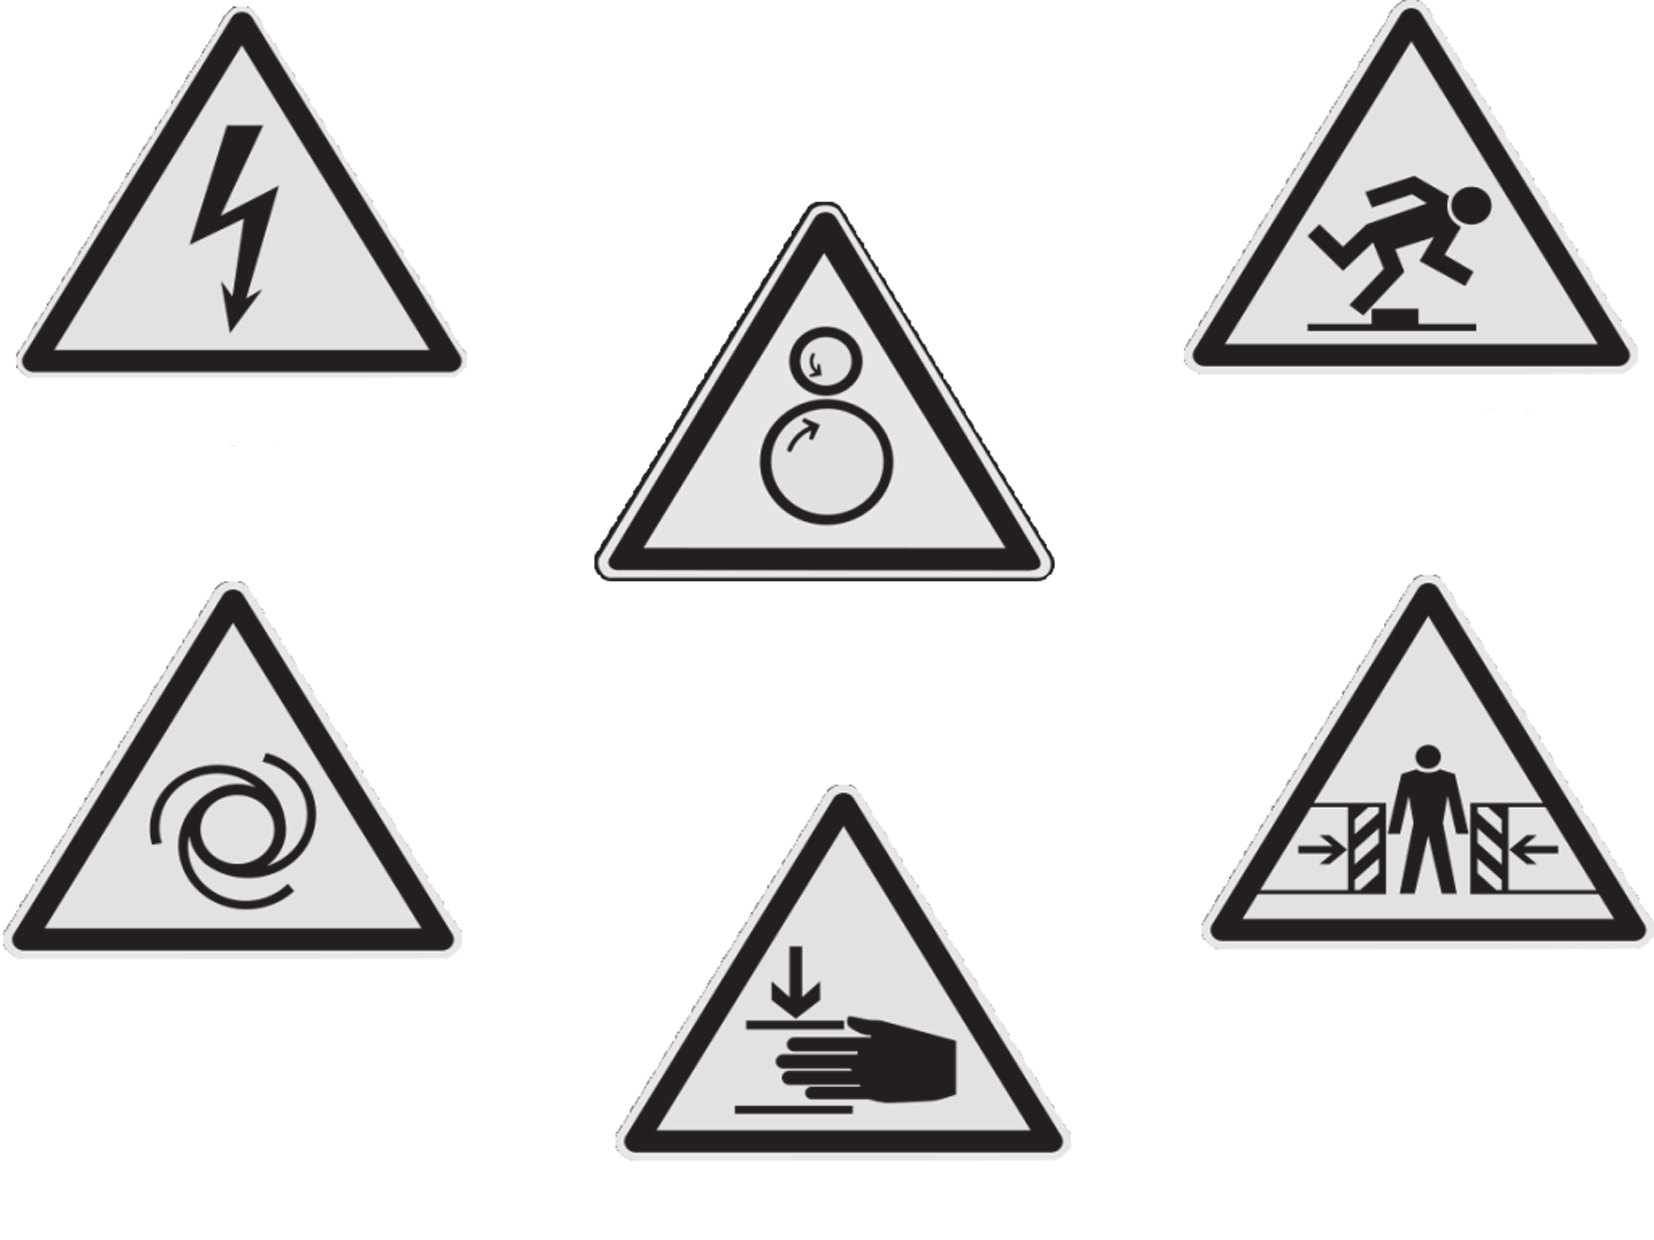
\includegraphics[width=0.82\textwidth]{img05-02.png}}
    \caption{Esempi di pericoli (fonte: Istituto tedesco di assicurazione sociale contro gli infortuni per il settore alimentare e della ristorazione).}
    \label{fig:05-02}
\end{figure}

\subsection{Valutazione del rischio}
\label{subsec:05-2-2}
A seguito della stima del rischio, viene eseguita una valutazione del rischio al fine di determinare se sia necessaria una riduzione del rischio. I criteri per un'adeguata riduzione del rischio sono specificati nella norma EN 12100~\cite{eniso12100}:
\begin{itemize}
    \item Sono state prese in considerazione tutte le condizioni operative e tutte le procedure di intervento?
    \item I pericoli sono stati eliminati mediante adeguate misure di protezione o i rischi sono stati ridotti al livello più basso possibile?
    \item È stato accertato che le misure adottate non creino nuovi pericoli?
    \item Gli utilizzatori sono stati sufficientemente informati e avvertiti dei rischi residui?
    \item È stato accertato che le misure di protezione adottate non compromettano le condizioni di lavoro degli operatori o l'usabilità della macchina?
    \item Le misure di protezione adottate sono compatibili tra loro?
    \item Sono state prese in debita considerazione le conseguenze che possono derivare dall'utilizzo, in un contesto non professionale/non industriale, di una macchina progettata per uso professionale/industriale?
\end{itemize}

\begin{figure}[htbp]
    \centering
    \resizebox{\textwidth}{!}{%==============================================================
%  Figura 5.3 - Stima del rischio e riduzione del rischio
%  Adattamento in italiano della Figura 5.3 dell'IFA Report 2/2017
%  Disegno vettoriale: coordinate in cm, origine sulla scala del rischio
%==============================================================
\begin{tikzpicture}[
  font=\footnotesize,
  fdline/.style={draw=black, line width=0.4pt},
  fdbox/.style={draw=black, fill=white, line width=0.4pt, align=center, inner sep=3pt},
  fdcall/.style={fdbox, rounded corners=4pt, text width=2.9cm, minimum height=1.45cm},
  fddash/.style={draw=black, line width=0.5pt, dash pattern=on 4pt off 3pt},
  lab/.style={font=\footnotesize, inner sep=1pt}
]

%--------------------------------------------------------------
% Scala del rischio (barra sfumata con punta a freccia)
%--------------------------------------------------------------
\shade[left color=white, right color=black] (0.64,-0.30) rectangle (12.34,0.30);
\fill[black] (12.34,-0.30) rectangle (14.55,0.30);
\draw[fdline] (0.64,-0.30) rectangle (14.55,0.30);
\filldraw[fill=white, draw=black, line width=0.4pt]
  (14.55,0.30) -- (14.55,0.72) -- (16.13,0) -- (14.55,-0.72) -- (14.55,-0.30) -- cycle;

% interruzione della scala
\fill[white] (1.80,-0.29) rectangle (2.24,0.29);
\draw[fdline] (1.78,-0.42) .. controls (2.02,-0.18) and (1.78,0.18) .. (2.02,0.42);
\draw[fdline] (1.98,-0.42) .. controls (2.22,-0.18) and (1.98,0.18) .. (2.22,0.42);

% tacche bianche in corrispondenza dei quattro livelli di rischio
\foreach \x in {4.44, 5.59, 8.39, 12.34}{
  \filldraw[fill=white, draw=black, line width=0.3pt] (\x-0.055,-0.30) rectangle (\x+0.055,0.30);
}

\node[lab, anchor=west] at (0.95,0.62) {basso};
\node[lab, anchor=west] at (13.55,0.62) {alto};

%--------------------------------------------------------------
% Fumetti dei quattro livelli di rischio
%--------------------------------------------------------------
\node[fdcall] (c1) at (3.03,2.17) {Rischio residuo\\ effettivo};
\node[fdcall] (c2) at (6.42,2.17) {Rischio accettabile/\\ tollerabile};
\node[fdcall] (c3) at (9.76,2.17) {Rischio senza\\ sistemi di comando\\ legati alla sicurezza};
\node[fdcall] (c4) at (13.17,2.17) {Rischio senza\\ misure di protezione};

\foreach \cx/\px in {3.03/4.44, 6.42/5.59, 9.76/8.39, 13.17/12.34}{
  \draw[fdline] (\cx-0.45,1.445) -- (\px,0.30);
  \draw[fdline] (\cx+0.45,1.445) -- (\px,0.30);
}

%--------------------------------------------------------------
% Linee tratteggiate di riferimento
%--------------------------------------------------------------
\foreach \x in {0.50, 4.44, 8.39, 12.34}{ \draw[fddash] (\x,-0.30) -- (\x,-6.95); }
\draw[fddash] (5.59,-0.30) -- (5.59,-4.62);

%--------------------------------------------------------------
% Frecce di riduzione del rischio
%--------------------------------------------------------------
\filldraw[fill=black!10, draw=black, line width=0.4pt]
  (12.34,-1.04) -- (7.20,-1.04) -- (7.20,-0.68) -- (5.59,-1.60)
  -- (7.20,-2.52) -- (7.20,-2.16) -- (12.34,-2.16) -- cycle;
\node[align=center, text width=5.0cm] at (9.77,-1.60)
  {Riduzione del rischio\\ minima necessaria};

\filldraw[fill=black!10, draw=black, line width=0.4pt]
  (12.34,-2.95) -- (6.05,-2.95) -- (6.05,-2.58) -- (4.44,-3.55)
  -- (6.05,-4.52) -- (6.05,-4.15) -- (12.34,-4.15) -- cycle;
\node[align=center, text width=5.6cm] at (9.20,-3.55)
  {Riduzione del rischio effettiva};

\node[lab, anchor=north west, align=left, text width=3.3cm] at (12.75,-0.80)
  {Rischio complessivo\\ presentato\\ dalla macchina};

%--------------------------------------------------------------
% Riquadri inferiori: ripartizione del rischio
%--------------------------------------------------------------
\node[draw=black, line width=0.5pt, dash pattern=on 4pt off 3pt, rounded corners=6pt,
      align=center, text width=3.4cm, minimum width=3.87cm, minimum height=2.16cm]
      (bA) at (2.505,-5.70) {Rischio residuo\\ rimanente};

\node[draw=black, line width=1.4pt, rounded corners=8pt,
      align=center, text width=3.3cm, minimum width=3.73cm, minimum height=2.16cm]
      (bB) at (6.455,-5.70) {Coperto dalle parti dei\\ sistemi di comando\\ legate alla sicurezza};

\node[draw=black, line width=0.4pt, rounded corners=2pt,
      align=center, text width=3.5cm, minimum width=3.80cm, minimum height=2.16cm]
      (bC) at (10.44,-5.70) {Coperto da misure\\ che non coinvolgono\\ le parti dei sistemi\\ di comando legate\\ alla sicurezza};

% interruzione del riquadro del rischio residuo
\foreach \y in {-4.62, -6.78}{
  \fill[white] (2.24,\y-0.06) rectangle (2.70,\y+0.06);
  \draw[fdline] (2.30,\y-0.16) .. controls (2.42,\y-0.06) and (2.18,\y+0.06) .. (2.30,\y+0.16);
  \draw[fdline] (2.50,\y-0.16) .. controls (2.62,\y-0.06) and (2.38,\y+0.06) .. (2.50,\y+0.16);
}

%--------------------------------------------------------------
% Cornice
%--------------------------------------------------------------
\draw[draw=black, line width=0.5pt]
  ([shift={(-0.40,0.40)}]current bounding box.north west) rectangle
  ([shift={(0.40,-0.40)}]current bounding box.south east);

\end{tikzpicture}
}
    \caption{Stima del rischio e riduzione del rischio.}
    \label{fig:05-03}
\end{figure}

\section{Identificazione delle funzioni di sicurezza}
\label{sec:05-3}
Qualora la valutazione identifichi un rischio (non ancora) inaccettabile, è necessario prevedere adeguate misure di sicurezza. La priorità deve tuttavia essere data agli sforzi volti a evitare i pericoli (progettazione intrinsecamente sicura) o, quantomeno, a ridurli il più possibile, mediante modifiche progettuali alla macchina. In linea di principio, anche le informazioni per l'uso (incluse le misure organizzative) rappresentano un possibile mezzo di riduzione del rischio. Misure di questo tipo sono tuttavia accettabili solo in casi eccezionali in cui non sia possibile una riduzione del rischio economicamente ragionevole mediante misure di protezione tecniche; nella maggior parte dei casi, tuttavia, saranno necessarie misure di sicurezza. In questo contesto, vengono definite le funzioni di sicurezza eseguite dal SRP/CS (parti dei sistemi di controllo relative alla sicurezza)
\begin{figure}[htbp]
    \centering
    \resizebox{0.8\textwidth}{!}{%==============================================================
%  Figura 5.4 - Le funzioni di sicurezza sono eseguite dagli SRP/CS
%  Adattamento in italiano della Figura 5.4 dell'IFA Report 2/2017
%==============================================================
\begin{tikzpicture}[
  font=\normalsize,
  blocco/.style={draw=black, line width=1pt, minimum width=3.4cm, minimum height=1.4cm,
                 align=center, inner sep=3pt, font=\large},
  freccia/.style={draw=black, line width=1pt, -{Triangle[length=6pt,width=6pt]}},
  didasc/.style={font=\normalsize, inner sep=2pt}
]

\node[blocco] (sensore)   at (2.0,0)  {Sensore};
\node[blocco] (logica)    at (6.4,0)  {Logica};
\node[blocco] (attuatore) at (10.8,0) {Attuatore};

\draw[freccia] (sensore.east) -- (logica.west);
\draw[freccia] (logica.east) -- (attuatore.west);

\node[didasc, below=0.55cm of sensore]   {Rilevamento};
\node[didasc, below=0.55cm of logica]    {Elaborazione};
\node[didasc, below=0.55cm of attuatore] {Commutazione};

\draw[draw=black, line width=1pt]
  ([shift={(-0.7,0.7)}]current bounding box.north west) rectangle
  ([shift={(0.7,-0.5)}]current bounding box.south east);

\end{tikzpicture}
}
    \caption{Le funzioni di sicurezza sono eseguite dagli SRP/CS.}
    \label{fig:05-04}
\end{figure}
Un processo iterativo per la progettazione delle parti dei sistemi di controllo relative alla sicurezza è descritto in~\cite{eniso13849-1}. La Figura~\ref{fig:05-05} mostra la parte pertinente a questa sotto clausola della relazione.
\begin{figure}[htbp]
    \centering
    \resizebox{\textwidth}{!}{%==============================================================
%  Figura 5.5 - Estratto del processo iterativo per la progettazione
%  delle parti dei sistemi di comando legate alla sicurezza (SRP/CS)
%  Adattamento in italiano della Figura 5.5 dell'IFA Report 2/2017
%==============================================================
\begin{tikzpicture}[
  font=\normalsize,
  grigio/.style={fill=black!10, align=center, inner sep=4pt},
  numcella/.style={draw=black, fill=white, line width=0.8pt,
                   minimum width=0.7cm, minimum height=0.75cm, inner sep=1pt},
  corpo/.style={draw=black, fill=black!10, line width=0.8pt,
                minimum width=9.0cm, minimum height=0.75cm, inner sep=3pt},
  fdline/.style={draw=black, line width=0.9pt},
  fdar/.style={fdline, -{Triangle[length=6pt,width=6pt]}}
]

%--------------------------------------------------------------
% Ingresso dall'analisi dei rischi
%--------------------------------------------------------------
\node[grigio, minimum width=4.2cm, minimum height=1.3cm] (analisi) at (2.5,-1.05)
  {Dall'analisi dei rischi\\ (EN ISO 12100)};

%--------------------------------------------------------------
% Le tre fasi numerate
%--------------------------------------------------------------
\foreach \n/\y/\testo in {%
  1/-2.65/{Identificazione delle funzioni di sicurezza (SF)},
  2/-3.95/{Specifica delle caratteristiche di ciascuna SF},
  3/-5.25/{Determinazione del PL richiesto (PL\textsubscript{r})}}{
  \node[numcella, anchor=west] (num\n) at (3.3,\y) {\n};
  \node[corpo, anchor=west] (fase\n) at (4.0,\y) {\testo};
}

%--------------------------------------------------------------
% Percorso principale
%--------------------------------------------------------------
\draw[fdar] (analisi.east) -- (5.30,-1.05) -- (5.30,-2.28);
\draw[fdar] (5.30,-3.03) -- (5.30,-3.58);
\draw[fdar] (5.30,-4.33) -- (5.30,-4.88);
\draw[fdar] (5.30,-5.63) -- (5.30,-6.45);

%--------------------------------------------------------------
% "Per ciascuna SF" con graffa
%--------------------------------------------------------------
\node[grigio, minimum width=1.5cm, minimum height=1.6cm] (perogni) at (1.15,-5.25)
  {Per\\ ciascuna\\ SF};
\draw[fdline, decorate, decoration={brace, amplitude=6pt}] (2.60,-5.95) -- (2.60,-4.55);

%--------------------------------------------------------------
% Uscite
%--------------------------------------------------------------
\node[align=center, text width=6.4cm] at (8.15,-7.25)
  {All'implementazione\\ e determinazione del PL\\ (Figura 6.1)};

\draw[fdline] (14.60,-6.45) -- (14.60,-3.95);
\draw[fdar] (14.60,-3.95) -- (13.00,-3.95);
\node[align=center, text width=2.8cm] at (14.60,-7.45)
  {Ritorno\\ se esistono\\ altre SF\\ (Figura 7.1)};

%--------------------------------------------------------------
% Cornice
%--------------------------------------------------------------
\draw[draw=black, line width=1pt]
  ([shift={(-0.45,0.45)}]current bounding box.north west) rectangle
  ([shift={(0.45,-0.45)}]current bounding box.south east);

\end{tikzpicture}
}
    \caption{Estratto del processo iterativo per la progettazione delle parti dei sistemi di comando legate alla sicurezza (SRP/CS).}
    \label{fig:05-05}
\end{figure}

\subsection{Definizione delle funzioni di sicurezza}
\label{subsec:05-3-1}
Le funzioni di sicurezza necessarie vengono definite tenendo conto sia dell'applicazione che del pericolo. Ad esempio, se si deve prevedere la proiezione di detriti, una barriera fotoelettrica non sarà una soluzione adeguata e sarà necessario un dispositivo di arresto (protezione). Una funzione di sicurezza è quindi una funzione mediante la quale le misure adottate (incluse quelle relative alla tecnologia di controllo) riducono il rischio presentato da un particolare pericolo a un livello accettabile. In assenza di disposizioni pertinenti in una norma di tipo C, le funzioni di sicurezza sono definite dal progettista della macchina, ad esempio:
\begin{enumerate} [label=\alph*)]
    \item arresto controllato del movimento e azionamento del freno di stazionamento in posizione di riposo
    \item prevenzione di schiacciamenti causati dalla caduta di parti della macchina
    \item iduzione della potenza del laser di taglio in caso di esposizione diretta dell'occhio
    \item prevenzione della caduta dell'albero in modalità di impostazione
    \item allontanamento del robot in caso di ingresso di una persona nella sua zona di pericolo
    \item prevenzione dell'intrappolamento di persone
    \item arresto del movimento di chiusura controllato da un azionamento a due mani in caso di intervento di una seconda persona nella zona di pericolo (attivato tramite una barriera fotoelettrica)
\end{enumerate}
Vengono spesso impiegate funzioni di sicurezza composite, come nell'esempio del punto~\ref{sec:05-7}. Il movimento viene inizialmente arrestato dal sistema di azionamento elettronico, dopodiché viene azionato un freno di stazionamento meccanico. Le due tabelle seguenti forniscono informazioni sulle possibili funzioni di sicurezza.

La Tabella~\ref{tab:05-1} riassume le funzioni di sicurezza secondo la sotto clausola 5.1 della norma EN ISO 13849-1 e aggiunge esempi di possibili applicazioni. È inclusa anche la “funzione di arresto di emergenza”: sebbene non faccia parte di una protezione, viene utilizzata per l’attuazione di una misura di protezione complementare (vedere la sotto clausola~\ref{sec:05-5}).

La Tabella~\ref{tab:05-2} mostra ulteriori funzioni di sicurezza per i sistemi di azionamento di potenza sicuri secondo la norma IEC 61800-5-2 (PDS/SR, sistemi di azionamento di potenza/relativi alla sicurezza)~\cite{iec61800-5-2}. L’ambito di applicazione di questa norma comprende le funzioni di sicurezza frequentemente impiegate per la prevenzione dell’avvio imprevisto (arresto sicuro della coppia, STO), per l’arresto sicuro SS1 e SS2 e per la velocità limitata in sicurezza (SLS).

Le funzioni di sicurezza per la tecnologia di azionamento pneumatico sono descritte nella norma tecnica VDMA 24584~\cite{vdma24584}.


\begingroup
\definecolor{tabblue}{RGB}{31,73,125}
\fontsize{9}{11}\selectfont
\setlength{\tabcolsep}{4pt}
\renewcommand{\arraystretch}{1.2}
\setlength{\LTcapwidth}{\textwidth}
\begin{longtable}{|p{5.8cm}|p{\dimexpr\textwidth-5.8cm-4\tabcolsep-4\arrayrulewidth\relax}|}
    \caption{Funzioni di sicurezza descritte in EN ISO 13849-1.}
    \label{tab:05-1} \\
    \hline
    \rowcolor{tabblue}
    \textcolor{white}{\textbf{Funzione di sicurezza}} & \textcolor{white}{\textbf{Esempio applicativo}} \\
    \hline
    \endfirsthead
    \hline
    \rowcolor{tabblue}
    \textcolor{white}{\textbf{Funzione di sicurezza}} & \textcolor{white}{\textbf{Esempio applicativo}} \\
    \hline
    \endhead
    \hline
    \endfoot
    Funzione di arresto legata alla sicurezza, avviata da un dispositivo di protezione &
    Risposta all'intervento di un dispositivo di protezione con STO, SS1 o SS2 (Tabella~\ref{tab:05-2}) \\
    \hline
    \rowcolor{black!8}
    Funzione di ripristino manuale &
    Confermare quando le aree dietro il dispositivo di protezione vengono liberate \\
    \hline
    Funzione di avvio/riavvio &
    Ammissibile solo con protezioni ad incastro con funzione di avviamento secondo la norma EN ISO 12100 \\
    \hline
    \rowcolor{black!8}
    Funzione di controllo locale &
    Controllo dei movimenti delle macchine da una postazione all'interno della zona di pericolo \\
    \hline
    Funzione di silenziamento &
    Disattivazione temporanea dei dispositivi di sicurezza, ad esempio durante il trasporto dei materiali \\
    \hline
    \rowcolor{black!8}
    Apparecchiatura a funzionamento continuo (interruttore a impulsi) &
    Movimenti della macchina controllati da una posizione all'interno della zona di pericolo, ad esempio durante la fase di impostazione \\
    \hline
    Funzione di abilitazione &
    Movimenti della macchina controllati da una posizione all'interno della zona di pericolo, ad esempio durante la fase di impostazione \\
    \hline
    \rowcolor{black!8}
    Prevenzione dell'avvio imprevisto &
    Intervento manuale dell'operatore nelle zone di pericolo \\
    \hline
    Fuga e salvataggio di persone intrappolate &
    Separazione dei rulli \\
    \hline
    \rowcolor{black!8}
    Funzione di isolamento e dissipazione dell'energia &
    Apertura di una valvola idraulica per lo scarico della pressione \\
    \hline
    Modalità di controllo e selezione della modalità operativa &
    Attivazione delle funzioni di sicurezza tramite un selettore di modalità operativa \\
    \hline
    \rowcolor{black!8}
    Funzione di arresto di emergenza &
    Risposta all'azionamento di un dispositivo di arresto di emergenza con STO o SS1 (Tabella~\ref{tab:05-2}) \\
    \hline
\end{longtable}
\endgroup

\begingroup
\definecolor{tabblue}{RGB}{31,73,125}
\fontsize{9}{11}\selectfont
\setlength{\tabcolsep}{4pt}
\renewcommand{\arraystretch}{1.2}
\setlength{\LTcapwidth}{\textwidth}
\begin{longtable}{|p{1.8cm}|p{4.2cm}|p{\dimexpr\textwidth-6cm-6\tabcolsep-5\arrayrulewidth\relax}|}
    % La didascalia breve (fra parentesi quadre) e' quella che finisce
    % nell'elenco delle tabelle: va tenuta priva di \cite, perche' li'
    % la citazione verrebbe eseguita nel frontespizio.
    \caption[Funzioni di sicurezza descritte nella norma IEC 61800-5-2 (edizione 2016)]{Funzioni di sicurezza descritte nella norma IEC 61800-5-2 (edizione 2016)~\cite{iec61800-5-2}.}
    \label{tab:05-2} \\
    \hline
    \rowcolor{tabblue}
    \textcolor{white}{\textbf{Sigla}} & \textcolor{white}{\textbf{Denominazione}} & \textcolor{white}{\textbf{Funzione}} \\
    \hline
    \endfirsthead
    \hline
    \rowcolor{tabblue}
    \textcolor{white}{\textbf{Sigla}} & \textcolor{white}{\textbf{Denominazione}} & \textcolor{white}{\textbf{Funzione}} \\
    \hline
    \endhead
    \hline
    \endfoot
    \rowcolor{black!8}
    STO & Coppia disinserita in sicurezza &
    Il motore non riceve energia in grado di generare un movimento rotatorio; arresto di categoria 0 secondo la norma EN 60204-1 \\
    \hline
    SS1-r \newline SS1-t & Arresto sicuro 1 &
    Motore in decelerazione; monitoraggio della rampa di decelerazione e STO al raggiungimento dell'arresto (SS1-r), oppure STO allo scadere di un tempo prestabilito (SS1-t); arresto di categoria 1 secondo la norma EN 60204-1 \\
    \hline
    \rowcolor{black!8}
    SS2-r \newline SS2-t & Arresto sicuro 2 &
    Motore in decelerazione; monitoraggio della rampa di decelerazione e SOS al raggiungimento dell'arresto (SS2-r), oppure SOS allo scadere di un tempo prestabilito (SS2-t); arresto di categoria 2 secondo la norma EN 60204-1 \\
    \hline
    SOS & Arresto operativo sicuro &
    Il motore è fermo e si oppone alle forze esterne \\
    \hline
    \rowcolor{black!8}
    SLA & Accelerazione limitata in sicurezza &
    Viene impedito il superamento di un valore limite di accelerazione e/o decelerazione \\
    \hline
    SLS & Velocità limitata in sicurezza &
    Viene impedito il superamento del valore limite di velocità \\
    \hline
    \rowcolor{black!8}
    SLT & Coppia limitata in sicurezza &
    Viene impedito il superamento di un valore limite di coppia/forza \\
    \hline
    SLP & Posizione limitata in sicurezza &
    Viene impedito il superamento di un valore limite di posizione \\
    \hline
    \rowcolor{black!8}
    SLI & Incremento limitato in sicurezza &
    Il motore viene spostato di una distanza incrementale prestabilita, al termine della quale si arresta \\
    \hline
    SDI & Direzione sicura &
    Si impedisce che il motore ruoti nella direzione non desiderata \\
    \hline
    \rowcolor{black!8}
    SMT & Temperatura sicura del motore &
    Viene impedito il superamento di un valore limite di temperatura del motore \\
    \hline
    SBC & Comando sicuro del freno &
    Azionamento sicuro di un freno esterno \\
    \hline
    \rowcolor{black!8}
    SCA & Camma sicura &
    Viene generato un segnale di uscita sicuro finché la posizione del motore rimane entro un intervallo prestabilito \\
    \hline
    SSM & Monitoraggio sicuro della velocità &
    Viene generato un segnale di uscita sicuro finché la velocità del motore rimane al di sotto di un valore prestabilito \\
    \hline
    \rowcolor{black!8}
    SAR & Intervallo di accelerazione sicuro &
    L'accelerazione del motore viene mantenuta entro valori limite prestabiliti \\
    \hline
    SSR & Intervallo di velocità sicuro &
    La velocità del motore viene mantenuta entro valori limite prestabiliti \\
    \hline
    \rowcolor{black!8}
    STR & Intervallo di coppia sicuro &
    La coppia del motore (la forza, nel caso di motori lineari) viene mantenuta entro valori limite prestabiliti \\
    \hline
\end{longtable}
\endgroup

Il modo in cui una funzione di sicurezza viene eseguita può assumere forme molto diverse. Per questo motivo, in fase di selezione occorre considerare determinate caratteristiche e specificarle caso per caso.

Tra queste:
\begin{itemize}
    \item utilizzo nelle diverse modalità operative (ad es. modalità automatica, modalità di predisposizione/setup, ricerca guasti) 
    \item utilizzo di diverse funzioni di sicurezza a seconda che l'alimentazione elettrica sia presente o sia venuta a mancare (vedere anche il paragrafo 4.3 di~\cite{werner2019}) 
    \item risposta/e all'intervento della funzione di sicurezza 
    \item risposta/e alla rilevazione di un guasto nella funzione di sicurezza 
    \item tempo di risposta 
    \item frequenza di attuazione 
    \item priorità, nei casi in cui più funzioni di sicurezza possano essere attive simultaneamente
    \item specifica dei parametri legati alla sicurezza, quali la velocità massima ammissibile
    \item performance Level richiesto PL\textsubscript{\small r}
\end{itemize}

Informazioni dettagliate sulla definizione delle funzioni di sicurezza sono disponibili nel SISTEMA Cookbook 6, "Definizione delle funzioni di sicurezza: cosa è importante?"~\cite{cookbook6}.

% \texorpdfstring serve perche' questo titolo finisce anche nei segnalibri
% del PDF, che accettano solo testo semplice: il primo argomento e' la resa
% tipografica, il secondo quella per il segnalibro.
\subsection{Esempi di definizione di funzioni di sicurezza con influenza sul successivo calcolo del \texorpdfstring{PFH\textsubscript{\small D}}{PFHD}}
\label{subsec:05-3-2}
Nei capitoli successivi verrà illustrato come calcolare la probabilità media di un guasto pericoloso per ora (PFH\textsubscript{D}) per una funzione di sicurezza. Le basi per questo calcolo vengono tuttavia poste in questa fase, con la definizione della funzione di sicurezza. Per sua natura, l'implementazione tecnica di una funzione di sicurezza determina il tipo e la scala dei componenti necessari. La definizione della funzione di sicurezza ha quindi un'influenza considerevole sulla determinazione dell'affidabilità relativa alla sicurezza. Questo verrà spiegato negli esempi seguenti.

\textit{Esempio 1}:\\
\textit{Funzione di sicurezza "Arresto all'apertura del cancello di protezione"} \\
Quando il cancello di protezione viene aperto, l'operatore della macchina ha accesso a una zona di pericolo in cui cinque azionamenti controllano i movimenti delle parti della macchina. L'apertura del cancello di protezione provoca l'arresto immediato di tutti e cinque gli azionamenti.
Quando si calcola successivamente il PFH\textsubscript{D} (Physical Functional Hierarchy Diagram), diagramma funzionale di sicurezza della funzione di sicurezza, vengono quindi sommati i valori PFH\textsubscript{D} dei seguenti blocchi:
	
\begin{itemize}
    \item monitoraggio della posizione del cancello di protezione, inclusi i componenti meccanici;
    \item logica;
    \item azionamento da 1 a 5;
\end{itemize}
Il calcolo potrebbe produrre un PFH\textsubscript{\small D} non più adeguato all'applicazione, anche se solo gli azionamenti 1 e 3 avviano movimenti pericolosi nella posizione istantanea dell'operatore e i restanti azionamenti vengono arrestati esclusivamente "funzionalmente". In questo caso, si raccomanda di considerare solo i movimenti che effettivamente presentano un pericolo ai fini della funzione di sicurezza e di riformulare la funzione di sicurezza tenendo conto degli azionamenti critici per la sicurezza dell'operatore. Il diagramma funzionale associato è mostrato nella Figura~\ref{fig:05-06}.

Se più di un azionamento è coinvolto nei movimenti pericolosi nella zona di pericolo in esame, i pericoli sono considerati sovrapposti. Se il numero di azionamenti da considerare è troppo elevato, la somma dei valori PFH\textsubscript{D} dei singoli azionamenti può nuovamente risultare in un PFH\textsubscript{D} totale troppo elevato per il PL richiesto dalla funzione di sicurezza. La norma rivista prevede la considerazione dei pericoli sovrapposti. Di conseguenza, i pericoli considerati nella funzione di sicurezza in questione possono, in determinate circostanze, essere ridotti a pericoli discreti, ovvero i movimenti pericolosi della macchina possono essere ridotti ai movimenti di parti discrete della macchina. La possibilità di ciò in un dato caso deve essere determinata durante la valutazione del rischio. A tal proposito, l'Allegato J della presente relazione e~\cite{apfeld2010} forniscono un supporto.

% figura ancorata qui: deve restare fra l'Esempio 1 e l'Esempio 2.
% Non e' un float (niente \begin{figure}), quindi LaTeX non puo'
% spostarla; \captionof fornisce la didascalia numerata.
% La minipage tiene insieme disegno e didascalia: una figura non
% fluttuante puo' spezzarsi a fine pagina, e senza di essa la
% didascalia finirebbe orfana sulla pagina successiva.
\begin{center}
    \begin{minipage}{\textwidth}
        \centering
        \captionsetup{hypcap=false}
        \resizebox{0.92\textwidth}{!}{%==============================================================
%  Figura 5.6 - Arresto degli azionamenti 1 e 3 all'apertura
%  del cancello di protezione
%  Adattamento in italiano della Figura 5.6 dell'IFA Report 2/2017
%
%  Le campiture grigie evidenziano cio' che rientra nella funzione
%  di sicurezza: monitoraggio del cancello, logica e azionamenti 1 e 3.
%  L'azionamento 2 e' ritagliato in bianco perche' resta fuori dalla
%  funzione, pur essendo collegato alla stessa linea di comando.
%==============================================================
\begin{tikzpicture}[
  font=\normalsize,
  blocco/.style={draw=black, line width=1.2pt, fill=white, align=center,
                 inner sep=4pt, minimum height=1.0cm},
  azionamento/.style={blocco, minimum width=3.4cm},
  collegamento/.style={draw=black, line width=0.8pt}
]

% ---- campiture: prima le aree grigie, poi il ritaglio bianco --------
\fill[black!8] (-0.45,1.25) rectangle (13.45,3.15);   % fascia orizzontale
\fill[black!8] (8.80,3.15) rectangle (13.45,5.75);    % braccio verticale
\fill[white]   (9.35,3.20) rectangle (13.45,4.35);    % ritaglio: azionamento 2

% ---- blocchi -------------------------------------------------------
\node[blocco, minimum width=5.6cm, minimum height=1.5cm] (cancello) at (3.0,2.2)
  {Monitoraggio della posizione\\del cancello di protezione};
\node[blocco, minimum width=2.0cm] (logica) at (7.2,2.2) {Logica};

\node[azionamento] (az1) at (11.3, 5.0) {Azionamento 1};
\node[azionamento] (az2) at (11.3, 3.6) {Azionamento 2};
\node[azionamento] (az3) at (11.3, 2.2) {Azionamento 3};
\node[azionamento] (az4) at (11.3, 0.8) {Azionamento 4};
\node[azionamento] (az5) at (11.3,-0.6) {Azionamento 5};

% ---- collegamenti --------------------------------------------------
\draw[collegamento] (cancello.east) -- (logica.west);
\draw[collegamento] (logica.east) -- (az3.west);       % logica -> azionamento 3
\draw[collegamento] (9.2,5.0) -- (9.2,-0.6);           % linea di distribuzione
\draw[collegamento] (9.2,5.0) -- (az1.west);
\draw[collegamento] (9.2,3.6) -- (az2.west);
\draw[collegamento] (9.2,0.8) -- (az4.west);
\draw[collegamento] (9.2,-0.6) -- (az5.west);

% ---- cornice esterna -----------------------------------------------
\draw[draw=black, line width=1.2pt]
  ([shift={(-0.55,0.45)}]current bounding box.north west) rectangle
  ([shift={( 0.55,-0.45)}]current bounding box.south east);

\end{tikzpicture}
}
        \captionof{figure}{Arresto degli azionamenti 1 e 3 all'apertura del cancello di protezione.}
        \label{fig:05-06}
    \end{minipage}
\end{center}

\textit{Esempio 2}:\\
\textit{Funzione di sicurezza "Arresto del movimento all'apertura di un cancello di protezione"} \\
Un movimento pericoloso è protetto da una recinzione con cinque cancelli di protezione. L'apertura di uno qualsiasi dei cancelli arresta il movimento. Poiché una persona aprirà sempre e solo un cancello di protezione alla volta, ciascun cancello costituisce una funzione di sicurezza a sé stante, da SF1 a SF5, composta dai seguenti blocchi:
\begin{itemize}
    \item monitoraggio della posizione del cancello di protezione x (x = 1, 2, ... 5), inclusi i componenti meccanici;
    \item logica;
\end{itemize}
La Figura~\ref{fig:05-07} mostra lo schema funzionale e i blocchi della funzione di sicurezza SF3

% figura ancorata qui: deve restare fra l'Esempio 2 e l'Esempio 3.
% Non e' un float (niente \begin{figure}), quindi LaTeX non puo'
% spostarla; \captionof fornisce la didascalia numerata.
% La minipage tiene insieme disegno e didascalia: una figura non
% fluttuante puo' spezzarsi a fine pagina, e senza di essa la
% didascalia finirebbe orfana sulla pagina successiva.
\begin{center}
    \begin{minipage}{\textwidth}
        \centering
        \captionsetup{hypcap=false}
        \resizebox{0.92\textwidth}{!}{%==============================================================
%  Figura 5.7 - Arresto dell'azionamento all'apertura del
%  cancello di protezione 3
%  Adattamento in italiano della Figura 5.7 dell'IFA Report 2/2017
%
%  Speculare alla Figura 5.6: qui il pericolo e' un solo azionamento,
%  sorvegliato da piu' cancelli. La fascia grigia isola il solo cancello 3
%  (con logica e azionamento), cioe' cio' che rientra nella funzione
%  di sicurezza in esame; gli altri cancelli restano fuori pur essendo
%  collegati alla stessa linea di comando.
%==============================================================
\begin{tikzpicture}[
  font=\normalsize,
  blocco/.style={draw=black, line width=1.2pt, fill=white, align=center,
                 inner sep=4pt, minimum height=1.0cm},
  cancello/.style={blocco, minimum width=5.8cm, minimum height=1.4cm},
  collegamento/.style={draw=black, line width=0.8pt}
]

% Coordinate della cornice, fissate esplicitamente: servono perche' la
% fascia grigia deve attraversare tutta la larghezza del riquadro, come
% nell'originale. Ricavandole dal bounding box si inseguirebbero a vicenda.
\def\cornicesx{-0.70}
\def\cornicedx{14.60}

% ---- campitura: la fascia della funzione di sicurezza --------------
\fill[black!8] (\cornicesx,2.40) rectangle (\cornicedx,4.00);

% ---- blocchi -------------------------------------------------------
\node[cancello] (p1) at (3.0, 6.4) {Monitoraggio della posizione\\del cancello di protezione 1};
\node[cancello] (p2) at (3.0, 4.8) {Monitoraggio della posizione\\del cancello di protezione 2};
\node[cancello] (p3) at (3.0, 3.2) {Monitoraggio della posizione\\del cancello di protezione 3};
\node[cancello] (p4) at (3.0, 1.6) {Monitoraggio della posizione\\del cancello di protezione 4};
\node[cancello] (p5) at (3.0, 0.0) {Monitoraggio della posizione\\del cancello di protezione 5};

\node[blocco, minimum width=2.2cm] (logica)      at (8.8, 3.2) {Logica};
\node[blocco, minimum width=3.4cm] (azionamento) at (12.2,3.2) {Azionamento};

% ---- collegamenti --------------------------------------------------
\draw[collegamento] (6.6,6.4) -- (6.6,0.0);          % linea di raccolta
\draw[collegamento] (p1.east) -- (6.6,6.4);
\draw[collegamento] (p2.east) -- (6.6,4.8);
\draw[collegamento] (p4.east) -- (6.6,1.6);
\draw[collegamento] (p5.east) -- (6.6,0.0);
\draw[collegamento] (p3.east) -- (logica.west);      % cancello 3 -> logica
\draw[collegamento] (logica.east) -- (azionamento.west);

% ---- cornice esterna -----------------------------------------------
\draw[draw=black, line width=1.2pt] (\cornicesx,-0.90) rectangle (\cornicedx,7.30);

\end{tikzpicture}
}
        \captionof{figure}{Arresto dell'azionamento all'apertura del cancello di protezione 3.}
        \label{fig:05-07}
    \end{minipage}
\end{center}

\textit{Esempio 3}:\\
\textit{Funzione di sicurezza 'Fermata di tutti gli azionamenti quando il dispositivo di arresto di emergenza viene azionato'}\\ 
Sono installati venti dispositivi di arresto di emergenza su una macchina di grandi dimensioni; quando azionati, essi arrestano tutti i 50 azionamenti nel modo più rapido possibile. Quali componenti devono essere considerati in questo caso durante l'implementazione della funzione di sicurezza? Non è possibile prevedere quale dei dispositivi di arresto di emergenza verrà azionato per attivare la funzione di sicurezza. Poiché l'utilizzatore aziona sempre un solo dispositivo di arresto di emergenza per volta, vengono definite le funzioni di sicurezza da SF1 a SF20. La posizione della persona esposta al pericolo nel momento in cui viene attivato l'arresto di emergenza non è nota. Indipendentemente da dove si trovi questa persona, tuttavia, non tutti i 50 azionamenti rappresentano un pericolo. Il caso peggiore dovrebbe pertanto essere considerato rappresentativo di tutte le situazioni ipotizzabili. Il caso peggiore viene determinato dal PFH\textsubscript{D} peggiore, e dipende quindi in parte dal numero di azionamenti nella catena di sicurezza che generano movimenti pericolosi nella posizione meno favorevole, e dai rispettivi valori individuali di PFH\textsubscript{D}\@. Il diagramma a blocchi associato è mostrato nella Figura~\ref{fig:05-08}. I valori PFH\textsubscript{D} dei seguenti blocchi devono pertanto essere presi in considerazione durante il successivo calcolo del PFH\textsubscript{D} della funzione di sicurezza:
\begin{itemize}
	\item dispositivo di arresto di emergenza 03
	\item logica
	\item azionamento 21
	\item azionamento 35
	\item azionamento 47
\end{itemize}

% La minipage tiene insieme disegno e didascalia: una figura non
% fluttuante puo' spezzarsi a fine pagina, e senza di essa la
% didascalia finirebbe orfana sulla pagina successiva.
\begin{center}
    \begin{minipage}{\textwidth}
        \centering
        \captionsetup{hypcap=false}
        \resizebox{0.92\textwidth}{!}{%==============================================================
%  Figura 5.8 - Arresto di emergenza dell'intera macchina,
%  caso peggiore
%  Adattamento in italiano della Figura 5.8 dell'IFA Report 2/2017
%
%  I dispositivi di arresto di emergenza sono venti e gli azionamenti
%  cinquanta: i puntini verticali e i tratti tratteggiati indicano gli
%  elementi non rappresentati. La campitura grigia isola il caso
%  peggiore, cioe' il dispositivo 03 con la logica e i soli azionamenti
%  21, 35 e 47, quelli che generano movimenti pericolosi nella
%  posizione meno favorevole.
%==============================================================
\begin{tikzpicture}[
  font=\normalsize,
  blocco/.style={draw=black, line width=1.2pt, fill=white, align=center,
                 inner sep=4pt, minimum height=0.9cm},
  dispositivo/.style={blocco, minimum width=7.2cm},
  azionamento/.style={blocco, minimum width=3.6cm},
  collegamento/.style={draw=black, line width=0.8pt},
  continua/.style={draw=black!55, line width=0.9pt, dash pattern=on 4pt off 4pt}
]

% Coordinate della cornice, fissate esplicitamente: le linee tratteggiate
% di continuazione devono poter arrivare fin quasi al bordo senza che il
% bordo, ricavato dal bounding box, le insegua.
\def\cornicesx{-0.55}
\def\cornicedx{17.10}
\def\cornicegiu{-0.75}
\def\cornicesu{7.85}

% ---- campiture: cio' che rientra nel caso peggiore -----------------
\fill[black!8] (-0.15,3.02) rectangle (16.90,4.18);   % fascia orizzontale
\fill[black!8] (12.60,0.55) rectangle (16.90,6.55);   % colonna azionamenti

% ---- blocchi: dispositivi di arresto di emergenza ------------------
\node[dispositivo] (d1) at (3.7,6.0) {Dispositivo di arresto di emergenza 01};
\node[dispositivo] (d2) at (3.7,4.8) {Dispositivo di arresto di emergenza 02};
\node[dispositivo] (d3) at (3.7,3.6) {Dispositivo di arresto di emergenza 03};
\node[dispositivo] (d4) at (3.7,2.4) {Dispositivo di arresto di emergenza 04};

\node[blocco, minimum width=2.2cm] (logica) at (10.3,3.6) {Logica};

% ---- blocchi: azionamenti ------------------------------------------
\node[azionamento] (a21) at (14.9,6.0) {Azionamento 21};
\node[azionamento] (a35) at (14.9,3.6) {Azionamento 35};
\node[azionamento] (a47) at (14.9,1.2) {Azionamento 47};

% ---- puntini di continuazione --------------------------------------
\foreach \y in {1.70,1.40,1.10} \fill[black] (3.7,\y) circle (1.7pt);
\foreach \y in {7.40,7.10,6.80} \fill[black] (14.9,\y) circle (1.7pt);
\foreach \y in {5.10,4.80,4.50} \fill[black] (14.9,\y) circle (1.7pt);
\foreach \y in {2.70,2.40,2.10} \fill[black] (14.9,\y) circle (1.7pt);
\foreach \y in {0.40,0.10,-0.20} \fill[black] (14.9,\y) circle (1.7pt);

% ---- collegamenti ---------------------------------------------------
% linea di raccolta dei dispositivi, con proseguimento tratteggiato
\draw[collegamento] (8.1,6.0) -- (8.1,2.4);
\draw[continua]     (8.1,2.4) -- (8.1,0.95);
\draw[collegamento] (d1.east) -- (8.1,6.0);
\draw[collegamento] (d2.east) -- (8.1,4.8);
\draw[collegamento] (d4.east) -- (8.1,2.4);
\draw[collegamento] (d3.east) -- (logica.west);      % dispositivo 03 -> logica

% linea di distribuzione agli azionamenti: tratteggiata per tutta
% l'altezza (gli azionamenti sono cinquanta), continua nel tratto servito
\draw[continua]     (12.6,\cornicegiu+0.25) -- (12.6,\cornicesu-0.25);
\draw[collegamento] (12.6,6.0) -- (12.6,1.2);
\draw[collegamento] (logica.east) -- (a35.west);
\draw[collegamento] (12.6,6.0) -- (a21.west);
\draw[collegamento] (12.6,1.2) -- (a47.west);

% ---- cornice esterna -------------------------------------------------
\draw[draw=black, line width=1.2pt]
  (\cornicesx,\cornicegiu) rectangle (\cornicedx,\cornicesu);

\end{tikzpicture}
}
        \captionof{figure}{Arresto di emergenza dell'intera macchina, caso peggiore.}
        \label{fig:05-08}
    \end{minipage}
\end{center}

Gli esempi mostrano il vantaggio di un 'approccio locale' per la definizione di una funzione di sicurezza, in cui vengono considerati:

\begin{itemize}
	\item in quale posizione si trovano le persone nel momento considerato per l'analisi?
	\item quali movimenti rappresentano pericoli nella posizione della/e persona/e?
    \item quali dispositivi di protezione attivano la funzione di sicurezza nel momento considerato per l'analisi?
\end{itemize}

\section{Determinazione del livello di Prestazione Richiesto \texorpdfstring{PL\textsubscript{\small r}}{PLr}}
\label{sec:05-4}
Per ogni funzione di sicurezza implementata\footnote{Il suffisso "r" (required, richiesto) indica che il Performance Level in questo caso è quello richiesto per la funzione di sicurezza (valore desiderato). La validazione, in una fase successiva, esamina se il PL raggiunto dal sistema di comando reale (valore effettivo) è maggiore o uguale al PL richiesto. In questo contesto, "maggiore di" significa: PL = e > PL = d > PL = c > PL = b > PL = a}  è necessario specificare un livello di prestazione richiesto PL\textsubscript{r} - in termini tecnici, il valore desiderato. I requisiti derivano dalla necessaria riduzione del rischio. Durante la definizione della riduzione del rischio, occorre considerare anche la probabilità e la gravità dell'incidente, che potrebbero non essere note.

La norma ISO/TR 14121-2~\cite{isotr14121-2} descrive i metodi per determinare la scala richiesta per la riduzione del rischio. La norma EN ISO 13849-1 utilizza uno di questi metodi, quello del grafico del rischio.

\subsection{Grafo del rischio}
\label{subsec:05-4-1}
Il diagramma nell'Allegato A della norma conduce direttamente al Livello di Prestazione PL\textsubscript{\small r} richiesto ed è spiegato di seguito (vedere Figura~
ef{fig:05-09}). Ulteriori esempi di determinazione del PL\textsubscript{\small r} sono reperibili nell'Allegato~\ref{app:A}.

% La minipage tiene insieme disegno e didascalia: una figura non
% fluttuante puo' spezzarsi a fine pagina, e senza di essa la
% didascalia finirebbe orfana sulla pagina successiva.
\begin{center}
    \begin{minipage}{\textwidth}
        \centering
        \captionsetup{hypcap=false}
        \resizebox{0.92\textwidth}{!}{%==============================================================
%  Figura 5.9 - Grafo del rischio per la determinazione del PLr
%  di ciascuna funzione di sicurezza
%  Adattamento in italiano della Figura 5.9 dell'IFA Report 2/2017
%
%  L'albero si legge da sinistra a destra: dal punto di partenza si
%  sceglie S (gravita' della lesione), poi F (frequenza e durata
%  dell'esposizione), poi P (possibilita' di evitare il pericolo).
%  Gli otto percorsi sfociano nei cinque riquadri del PLr richiesto:
%  a, b, b, c, c, d, d, e dall'alto verso il basso. Il cuneo grigio
%  centrale indica che il rischio cresce scendendo nel grafo.
%
%  Le quote verticali sono fissate esplicitamente perche' le frecce
%  dei percorsi devono entrare orizzontalmente nel riquadro corretto:
%  i riquadri sono alti 2 unita' e contigui (a: 8-10, b: 6-8,
%  c: 4-6, d: 2-4, e: 0-2), le foglie stanno dentro quegli intervalli.
%==============================================================
\begin{tikzpicture}[
  font=\normalsize,
  ramo/.style={draw=black, line width=1.2pt},
  freccia/.style={ramo, -{Triangle[length=7pt,width=7pt]}},
  etichetta/.style={font=\normalsize, inner sep=2pt},
  plr/.style={draw=black, line width=1.2pt, fill=white, inner sep=0pt,
              minimum width=1.8cm, minimum height=2.0cm, font=\large}
]

% ---- cuneo del rischio (disegnato per primo: le frecce gli passano sopra)
\fill[black!10] (10.4,10.2) -- (11.2,0.0) -- (9.6,0.0) -- cycle;
\node[etichetta, align=center, anchor=south] at (10.4,10.35) {Rischio\\basso};
\node[etichetta, align=center, anchor=north] at (10.4,-0.15) {Rischio\\alto};

% ---- punto di partenza ---------------------------------------------
\fill[black] (0,5.0) circle (5pt);
\node[etichetta, align=center, text width=3.2cm, anchor=east]
     at (-0.35,5.0) {Punto di partenza\\per la stima della\\riduzione del rischio};
\draw[ramo] (0,5.0) -- (1.2,5.0);

% ---- diramazione S: gravita' della lesione --------------------------
\draw[ramo] (1.2,7.125) -- (1.2,2.875);
\draw[freccia] (1.2,7.125) -- (2.7,7.125);
\draw[freccia] (1.2,2.875) -- (2.7,2.875);
\node[etichetta, above] at (1.85,7.125) {$S_1$};
\node[etichetta, above] at (1.85,2.875) {$S_2$};

% ---- diramazione F: frequenza e durata dell'esposizione -------------
\draw[ramo] (2.7,8.25) -- (2.7,6.0);
\draw[freccia] (2.7,8.25) -- (4.3,8.25);
\draw[freccia] (2.7,6.0)  -- (4.3,6.0);
\node[etichetta, above] at (3.4,8.25) {$F_1$};
\node[etichetta, above] at (3.4,6.0)  {$F_2$};

\draw[ramo] (2.7,4.0) -- (2.7,1.75);
\draw[freccia] (2.7,4.0)  -- (4.3,4.0);
\draw[freccia] (2.7,1.75) -- (4.3,1.75);
\node[etichetta, above] at (3.4,4.0)  {$F_1$};
\node[etichetta, above] at (3.4,1.75) {$F_2$};

% ---- diramazione P: possibilita' di evitare il pericolo -------------
% e percorso fino al riquadro del PLr
\draw[ramo] (4.3,9.0) -- (4.3,7.5);
\draw[ramo] (4.3,6.5) -- (4.3,5.5);
\draw[ramo] (4.3,4.5) -- (4.3,3.5);
\draw[ramo] (4.3,2.5) -- (4.3,1.0);

\foreach \y/\p in {9.0/1, 7.5/2, 6.5/1, 5.5/2, 4.5/1, 3.5/2, 2.5/1, 1.0/2} {
  \draw[freccia] (4.3,\y) -- (12.6,\y);
  \node[etichetta, above] at (5.0,\y) {$P_\p$};
}

% ---- riquadri del Performance Level richiesto ------------------------
\node[plr] at (13.5,9.0) {a};
\node[plr] at (13.5,7.0) {b};
\node[plr] at (13.5,5.0) {c};
\node[plr] at (13.5,3.0) {d};
\node[plr] at (13.5,1.0) {e};
\node[etichetta, align=center, anchor=south] at (13.5,10.35)
     {Livello di Prestazione\\richiesto PL\textsubscript{\small r}};

% ---- cornice esterna --------------------------------------------------
\draw[draw=black, line width=1.2pt]
  ([shift={(-0.6,0.6)}]current bounding box.north west) rectangle
  ([shift={(0.6,-0.5)}]current bounding box.south east);

\end{tikzpicture}
}
        \captionof{figure}{Grafo del rischio per la determinazione del PL\textsubscript{\small r} di ciascuna funzione di sicurezza.}
        \label{fig:05-09}
    \end{minipage}
\end{center}

Dal punto di partenza, vengono valutati i seguenti parametri di rischio\footnote{La probabilità di accadimento di un evento pericoloso viene analizzata congiuntamente al parametro di rischio P.}:
\begin{itemize}
    \item S - gravità della lesione
    \item F - frequenza e/o durata dell'esposizione al pericolo
    \item P - possibilità di evitare il pericolo o di limitare il danno
\end{itemize}
Il grafico del rischio conduce quindi al PL\textsubscript{\small r} necessario. Questa analisi deve essere eseguita per ciascuna funzione di sicurezza e senza considerare la riduzione del rischio che ne consegue. Qualora siano presenti altre misure tecniche implementate indipendentemente dal sistema di comando, come una protezione meccanica o ulteriori funzioni di sicurezza, se ne può presumere l'efficacia ai fini della determinazione del PL\textsubscript{\small r} richiesto. In tal caso, il PL\textsubscript{\small r} richiesto può essere ridotto di un livello.
\textit{Gravità della lesione S1 e S2}
In generale, la gravità della lesione (parametro S) in una zona pericolosa risulta variare ampiamente. Tuttavia, ai fini dei requisiti per il sistema di comando, è rilevante solo la seguente distinzione:
\begin{itemize}
    \item S1 - lieve (lesione normalmente reversibile)
    \item S2 - grave (lesione normalmente irreversibile o morte)
\end{itemize}
Per determinare la scelta tra S1 e S2 occorre tenere conto delle normali conseguenze degli infortuni e dei normali processi di guarigione.
Frequenza e/o esposizione al pericolo F1 e F2 (parametro F)
La frequenza e/o l'esposizione al pericolo vengono valutate come:
\begin{itemize}
    \item F1 - da rara a poco frequente, e/o tempo di esposizione breve
    \item F2 - grave (lesione normalmente irreversibile o morte)
\end{itemize}

Si tiene quindi conto sia del numero di interventi nella zona pericolosa in un determinato periodo, sia della durata della presenza al suo interno. La norma facilita la decisione stabilendo che, laddove gli interventi dell'operatore si verifichino più spesso di una volta ogni 15 minuti, deve essere scelto F2. In tutti gli altri casi, la scelta corretta è F1, a condizione che la durata dell'esposizione al pericolo non superi 1/20 del tempo di funzionamento totale della macchina. Durante la valutazione, occorre considerare un valore medio per la durata dell'esposizione al pericolo in relazione al tempo complessivo di utilizzo della macchina.

Per una pressa per lavorazione dei metalli caricata manualmente, il cui operatore deve intervenire ciclicamente tra gli stampi della pressa, F2 è chiaramente la scelta appropriata. Al contrario, per un centro di lavorazione che viene predisposto una sola volta all'anno e successivamente funziona in modo automatico, verrà senza dubbio scelto F1. Per la valutazione della frequenza e della durata dell'esposizione al pericolo, i casi in cui è esposta la stessa persona o persone diverse devono essere trattati allo stesso modo.

\textit{P - possibilità di evitare il pericolo P1 e P2 (parametro P)}
A questo punto, occorre valutare se il riconoscimento e l'elusione di una situazione pericolosa siano:

\begin{itemize}
    \item P1 - possibili in determinate condizioni
    \item P2 - appena possibili
\end{itemize}

Gli aspetti rilevanti per la definizione di questo parametro includono le caratteristiche fisiche della macchina, la qualifica dell'operatore e la sua possibile reazione. Se, ad esempio, la macchina deve essere predisposta mentre è in funzione a velocità limitata, il parametro P1 sarà la scelta corretta in presenza di bassi valori di accelerazione durante la predisposizione: con l'emergere lento dei pericoli e a condizione che vi sia sufficiente libertà di movimento, l'operatore sarà in grado di allontanarsi dalla zona pericolosa. Al contrario, deve essere scelto P2 quando è possibile raggiungere rapidamente velocità più elevate e l'operatore non ha alcuna reale possibilità di evitare un infortunio. Durante questa valutazione, si deve tenere conto solo della limitazione del pericolo mediante mezzi fisicamente possibili, e non della limitazione ottenuta tramite componenti di comando, poiché questi ultimi potrebbero guastarsi in caso di guasto. Ad esempio, dei rulli che si muovono in direzione della mano dell'operatore non possono intrappolarla in condizioni prive di guasti. In caso di guasto del sistema di comando, tuttavia, la direzione di rotazione potrebbe invertirsi e, nelle condizioni più sfavorevoli, la mano verrebbe trascinata all'interno.

Un ulteriore fattore che influenza la determinazione del PL\textsubscript{r} è la probabilità del verificarsi di un evento pericoloso (\cite{eniso12100}, 5.5.2.3.2). In questo contesto possono essere fattori determinanti il comportamento umano e il guasto tecnico. Entrambi sono difficili da stimare numericamente. La norma indica, tuttavia, i seguenti criteri esemplificativi:

\begin{itemize}
    \item Affidabilità dei dati
    \item Storico degli infortuni su macchine comparabili
\end{itemize}

La probabilità del verificarsi di un evento pericoloso viene analizzata congiuntamente al parametro di rischio P. Laddove esistano fattori che consentano di ritenere "bassa" la probabilità del verificarsi di un evento pericoloso, il PL\textsubscript{r} può essere ridotto di un livello; non deve tuttavia scendere al di sotto di PL a.

Quale motivazione può ora essere addotta per una classificazione "bassa"? La considerazione dei dati di affidabilità si riferisce (tra gli altri aspetti) al sistema di comando legato al processo (cioè non legato alla sicurezza). Il costruttore della macchina deve pertanto valutare, a questo scopo, se per la propria macchina si possa presumere anche un'elevata affidabilità dei componenti (elevato MTTF, in questo caso senza "D"). Quanto è quindi elevata, ad esempio, la probabilità che un PLC standard per il comando funzionale di una macchina avvii in modo errato un'attivazione inaspettata di un azionamento? Come devono essere valutati i componenti nuovi che presentano buoni valori di MTTF ma con i quali non è ancora stata acquisita esperienza pratica? Le condizioni di impiego dei PLC e dei componenti associati (sensori, inverter di frequenza, alimentatori, ecc.) sono comparabili con le applicazioni consuete? Quali sono le caratteristiche della rete di alimentazione? Potrebbero verificarsi interferenze elettromagnetiche elevate nel luogo di utilizzo previsto per la macchina? Quali sono le temperature prevalenti? Ecc. Fattori come questi possono aumentare la probabilità di guasto, anche qualora non vengano violati i limiti specificati dei componenti utilizzati. Esiste inoltre la possibilità di errori nel software, che ovviamente possono a loro volta dare origine a eventi pericolosi.

Laddove l'incidenza e la gravità degli infortuni su macchine comparabili, con rischi identici, medesimo concetto operativo e di sicurezza e dispositivi di protezione identici, siano note e vengano considerate basse, anche la probabilità del verificarsi di un evento pericoloso può essere classificata come bassa.

Il PL\textsubscript{\small r} ridotto in base a queste considerazioni non deve in nessun caso essere inferiore a quello delle macchine prese come riferimento per il confronto, poiché da una bassa incidenza e gravità degli infortuni non consegue che il livello di sicurezza fornito dalle funzioni di sicurezza implementate sia superiore a quello richiesto. Non è possibile prevedere se una riduzione del livello esistente comporterebbe un aumento inaccettabile dell'incidenza e della gravità degli infortuni.

Il capitolo~\ref{cap:06} descrive la successiva progettazione delle funzioni di sicurezza.

\section{Misure di protezione complementari}
\label{sec:05-5}
I requisiti per le misure di protezione complementari sono contenuti nella norma EN ISO 12100~\cite{eniso12100}, sotto-clausola 6.3.5. Per quanto riguarda le problematiche relative alla tecnologia di controllo trattate nella presente relazione, tali misure di protezione complementari includono in particolare:

\begin{itemize}
    \item misure per l'arresto in condizioni di emergenza
    \item inversione dei movimenti
    \item sezionamento e disspipazione dell'energia
\end{itemize}

Secondo la definizione, queste non costituiscono misure di protezione tecniche la cui implementazione richiederebbe un determinato Performance Level. Tali misure di protezione complementari dovrebbero tuttavia intervenire quando le misure di protezione tecniche (protezioni e/o dispositivi di protezione) hanno fallito o sono state elusive. Proprio in questi casi, ci si aspetta ad esempio che una funzione di arresto di emergenza sia effettivamente utilizzabile. Devono pertanto essere osservati i requisiti posti dalla IEC 60204-1~\cite{iec60204-1} riguardo ai circuiti di comando e alle funzioni di comando delle macchine. Il paragrafo 9.4, "Funzioni di comando in caso di guasto", richiede un livello adeguato di prestazione di sicurezza, che deve essere definito mediante la valutazione del rischio della macchina. In definitiva, quindi, i requisiti della EN ISO 13849 si applicano anche a queste misure di protezione complementari. Le misure di protezione complementari non devono in nessun caso influenzare la funzione e lo standard dei dispositivi di protezione.

\section{Trattamento dei macchinari obsoleti}
\label{sec:05-6}
In questo contesto, per macchinari obsoleti si intendono le macchine immesse sul mercato prima dell'entrata in vigore della Direttiva Macchine. A queste macchine non si applicano i requisiti della direttiva. Tuttavia, la sua applicazione potrebbe rendersi necessaria qualora i macchinari obsoleti vengano ampliati, modificati, modernizzati, ecc. In tali casi, occorre valutare se si sia verificata una modifica essenziale. In tal caso, i requisiti della Direttiva Macchine CE si applicano ai macchinari 'vecchi', ovvero obsoleti, allo stesso modo dei macchinari nuovi. Tali requisiti includono l'applicazione della norma EN ISO 13849. Un documento interpretativo redatto dal Ministero federale tedesco del lavoro e degli affari sociali (BMAS) aiuta a determinare se si sia verificata una modifica essenziale~\cite{modifichesostanziali}.

\section{Riduzione del rischio di una ghigliottina per il taglio della carta con ridondanza diversificata nel controllo logico (Categoria 4 - PL e)}
\label{sec:05-7}
L'esempio riportato in questo paragrafo illustra l'applicazione della EN ISO 13849-1 su una taglierina per carta. Verranno considerati in dettaglio solo alcuni aspetti, e non l'intero processo.
\begin{figure}[htbp]
    \centering
    \fbox{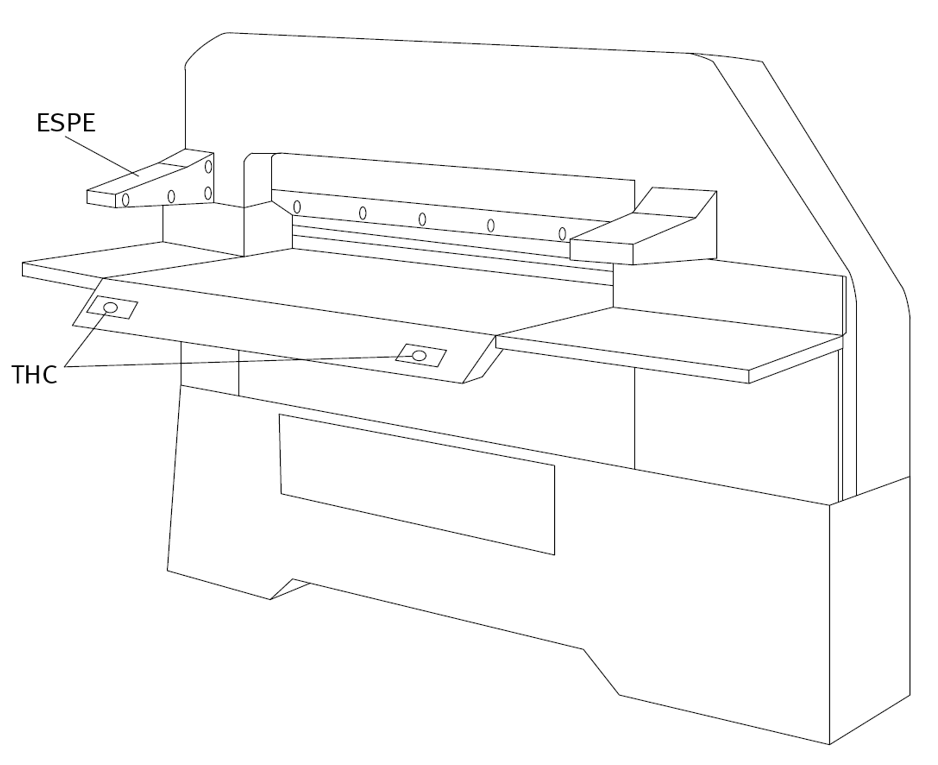
\includegraphics[width=0.75\textwidth]{img05-10.png}}
    \caption{Taglierina/ghigliottina per carta con comando bimanuale (THC) e attrezzatura di protezione elettrosensibile (ESPE -- AOPD).}
    \label{fig:05-10}
\end{figure}

Le taglierine per carta (vedi Figura~\ref{fig:05-10}) vengono utilizzate per tagliare pile di fogli di carta o materiali simili per mezzo di una lama. Il prodotto da tagliare viene generalmente posizionato sotto la lama manualmente. Immediatamente prima dell'esecuzione del taglio, una barra premi-pila viene abbassata con elevata forza sulla pila per tenerla ferma durante il taglio. La lama e la barra premi-pila sono azionate idraulicamente.

\subsection{Definizione dei limiti della macchina}
\label{subsec:05-7-1}

\textit{Limiti di spazio}
Poiché le taglierine per carta vengono caricate manualmente, è necessario uno spazio sufficiente per la movimentazione del prodotto da tagliare, per il successivo trasporto e stoccaggio della pila di carta tagliata, e per lo smaltimento degli scarti di carta, nonché uno spazio sufficiente per il movimento dell'operatore.

\textit{Limiti di tempo}
A seconda dell'applicazione, la macchina può essere utilizzata per un periodo di circa 20 anni. L'usura dei componenti può allungare il tempo necessario all'arresto di un movimento. La conseguente violazione della corsa di arresto deve pertanto essere rilevata e deve comportare l'arresto della macchina.

\textit{Limiti di utilizzo}
L'uso previsto della macchina è quello di tagliare pile di fogli di carta o materiali simili. La macchina viene caricata manualmente da una singola persona. A seconda del luogo di installazione e della larghezza della macchina, tuttavia, non può essere esclusa la presenza di altre persone nelle vicinanze.

Sono implementate le seguenti modalità operative:
\begin{enumerate}
    \item presatura
    \item taglio manuale (taglio singolo)
    \item sequenza automatica di tagli (processo automatico successivo al primo taglio manuale)
    \item cambio lama
\end{enumerate}

Nelle prime tre modalità operative è possibile il movimento della sola barra premi-pila, al fine di indicare la linea di taglio. A tale scopo, l'operatore aziona un pedale ed è in grado, contemporaneamente, di modificare la posizione della pila di carta con le mani all'interno della zona pericolosa.

\subsection{Identificazione dei pericoli}
\label{subsec:05-7-2}
I seguenti pericoli meccanici sono significativi per una taglierina per carta:
\begin{itemize}
    \item G1 - schiacciamento da parte della barra premi-pila
    \item G2 - taglio da parte della lama durante il processo di taglio
    \item G3 - taglio da parte della lama in posizione di riposo
\end{itemize}

\textit{Stima del rischio}
La forza dinamica di pressione della barra premi-pila (pericolo G1) è sufficientemente elevata da causare non solo lesioni da schiacciamento reversibili, ma anche fratture ossee. Per il pericolo G2, si deve presumere l'amputazione degli arti. Durante il posizionamento manuale della pila di carta, il pericolo G3 può causare lesioni alle mani o agli avambracci a contatto con la lama ferma. Queste lesioni sono tuttavia generalmente reversibili.

Il livello di esposizione al pericolo degli operatori è molto elevato, poiché essi intervengono manualmente in modo regolare (ciclico) nella zona pericolosa nel corso del normale lavoro.

Le velocità di discesa della barra premi-pila e della lama (pericoli G1 e G2) sono molto elevate, con la conseguenza che l'operatore non dispone praticamente di alcun mezzo per evitare il pericolo. Quando la lama è ferma (pericolo G3), l'operatore è in grado di evitare o limitare il danno.

La probabilità del verificarsi di un evento pericoloso a seguito di un guasto tecnico non è nota. L'incidenza e la gravità su macchine comparabili sono tuttavia basse; i dispositivi di protezione qui implementati risultano quindi evidentemente adeguati.

Qualora l'analisi del rischio per una funzione di sicurezza fornisse un PL\textsubscript{r} superiore a quello effettivamente implementato sulle macchine comparabili, il PL\textsubscript{\small r} potrebbe in linea di principio essere ridotto di un livello.

Tuttavia, poiché sulle taglierine per carta comparabili le funzioni di sicurezza vengono realizzate con il PL più elevato, in questo caso non sarà possibile alcuna riduzione del PL\textsubscript{\small r} (vedi paragrafo~\ref{subsec:05-7-4}).

\textit{Valutazione del rischio}
Considerando tutte le condizioni operative e tutte le possibilità di intervento dell'operatore, si riscontra la necessità di una riduzione del rischio.

\textit{Progettazione intrinsecamente sicura}
Non è possibile ridurre la forza dinamica di pressione della barra premi-pila e l'energia della lama, poiché ciò comprometterebbe la funzionalità della macchina. Non è inoltre possibile una disposizione e progettazione della macchina tale da impedire all'operatore di accedere con le mani alla zona pericolosa, poiché è proprio in quel punto che l'operatore deve allineare la pila di carta.

Possono tuttavia essere adottate le seguenti misure:
\begin{enumerate}
    \item schermatura di tutti i punti di accesso alla zona pericolosa, ad eccezione del lato operatore.
    \item eliminazione di spigoli e angoli taglienti.
    \item garanzia di una posizione di lavoro adeguata e dell'accessibilità dei comandi.
    \item progettazione ergonomica della macchina.
    \item eliminazione dei pericoli elettrici.
    \item eliminazione dei pericoli presentati dall'impianto idraulico.
    \item i componenti meccanici per la guida della lama e della barra premi pila sono collegati in modo tale che, nella posizione di riposo superiore, la lama sia schermata dalla barra premi pila
\end{enumerate}

\subsection{Funzioni di sicurezza richieste}
\label{subsec:05-7-3}
Tenendo conto di tutte le modalità operative e di tutti gli interventi manuali, sono richieste le seguenti funzioni di sicurezza:
\begin{itemize}
    \item SF1 - STO (Safe Torque Off), per evitare l'avviamento inatteso;
    \item SF2 - Posizionamento controllato delle mani dell'operatore al di fuori della zona pericolosa durante un movimento pericoloso;
    \item SF3 - Rilevamento dell'intervento di altre persone nella zona pericolosa mediante ESPE (attrezzatura di protezione elettrosensibile), ad es. una barriera fotoelettrica, e interruzione immediata dell'operazione di taglio;
    \item SF4 - Arresto automatico di tutti i movimenti dopo ogni singolo taglio o al termine della sequenza di taglio automatica;
    \item SF5 - Riduzione della forza dinamica di pressione della barra di serraggio durante la funzione "indicazione del taglio;
    \item SF6 - Ritorno automatico della barra di serraggio e della lama alle rispettive posizioni iniziali in seguito all'interruzione di un'operazione di taglio;
\end{itemize}

Nota: Il principio dei pericoli sovrapposti potrebbe essere applicato alle parti della macchina costituite dalla lama e dalla barra di serraggio (vedere il sottopunto~\ref{subsec:05-3-2}). In questo caso, le funzioni SF1, SF3, SF4 e SF6 verrebbero suddivise in modo tale da definire funzioni di sicurezza dedicate separatamente per la lama e per la barra di serraggio. Nel caso in esame, tuttavia, questa suddivisione non viene effettuata, poiché, a causa del basso numero di componenti presenti in SF1-SF6, il PFH\textsubscript{D} richiesto può comunque essere raggiunto raggruppando tali funzioni di sicurezza.

\textit{Caratteristiche delle funzioni di sicurezza}
Il taglio deve essere interrotto immediatamente qualora la barriera fotoelettrica venga oltrepassata. La funzione di sicurezza SF3 ha pertanto priorità rispetto a SF2. Per SF5, deve essere specificata la forza massima consentita per la barra di serraggio durante la funzione "indicazione del taglio" (vedere~\cite{en1010-3}).

\subsection{Determinazione del livello di prestazione richiesto \texorpdfstring{PL\textsubscript{r}}{PLr}}
\label{subsec:05-7-4}
Il PL\textsubscript{r} deve essere determinato per ciascuna funzione di sicurezza. Analizzando le situazioni in cui vengono utilizzate le singole funzioni di sicurezza, si osserva che la valutazione dei parametri di rischio S, F e P risulta simile per le funzioni di sicurezza da SF1 a SF6:
	\begin{itemize}
    \item S2 - lesione grave, generalmente irreversibile;
    \item F2 - presenza continua nella zona di pericolo; la frequenza è pertanto superiore a una volta ogni 15 minuti;
    \item P2 - la possibilità di sottrarsi alla situazione pericolosa è praticamente nulla;
\end{itemize}

In conformità al grafico di rischio della Figura~\ref{fig:05-09}, questa valutazione determina un Performance Level richiesto PL\textsubscript{r} pari a e. L'incidenza e la gravità degli infortuni su macchine comparabili sono basse. Le funzioni di sicurezza qui considerate per queste macchine sono già state realizzate con PL e, come specificato in~\cite{en1010-1}. Il risultato dell'analisi del rischio è quindi confermato dall'esperienza operativa; una possibile riduzione del PL\textsubscript{r} non è giustificata. La Figura~\ref{fig:05-11} mostra la documentazione e il grafico di rischio nell'applicazione software SISTEMA per la funzione di sicurezza SF1.

Per il pericolo G3, "Taglio da parte della lama in stato di riposo", è stata ottenuta una riduzione del rischio adeguata mediante l'accoppiamento meccanico della lama e della barra di pressione. Non è richiesta una funzione di sicurezza.

\begin{figure}[htbp]
    \centering
    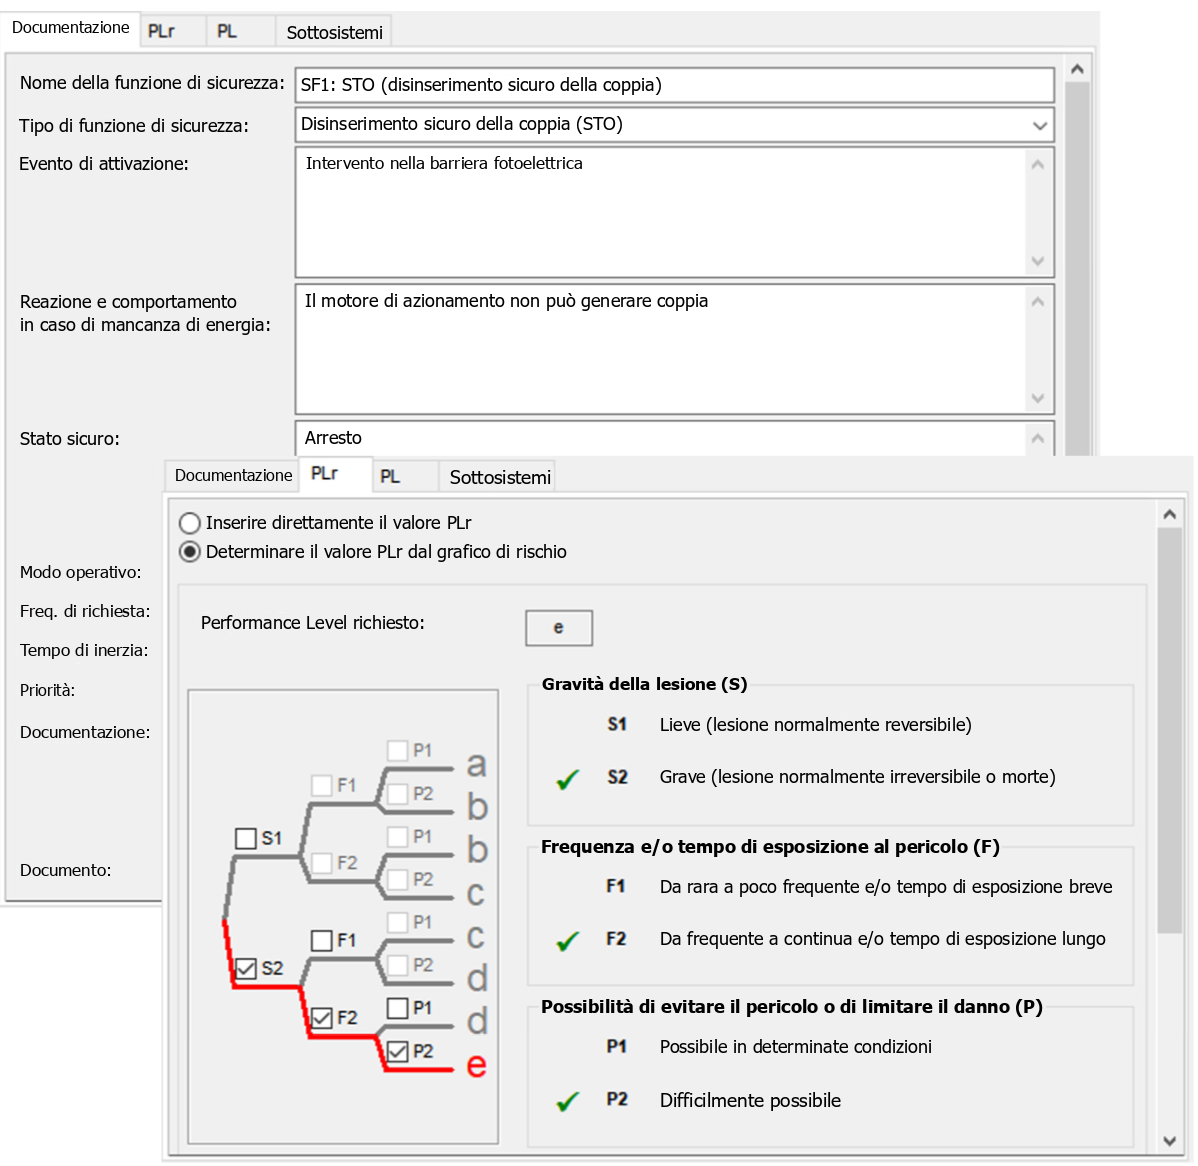
\includegraphics[width=0.85\textwidth]{img05-11.png}
    \caption{Documentazione e grafico di rischio per la SF1.}
    \label{fig:05-11}
\end{figure}

\subsection{Misure di protezione complementari}
\label{subsec:05-7-5}
Sono necessarie le seguenti misure:
\begin{enumerate}
    \item Arresto di emergenza. Nel sistema di comando della macchina sono già disponibili funzioni di sicurezza idonee con PL e, utilizzate per l'arresto di emergenza. A condizione che il dispositivo di arresto di emergenza disponga di un circuito a due canali, anche l'arresto in caso di emergenza soddisfa quindi il PL e.
    \item La liberazione di una persona intrappolata richiede un movimento di ritorno della lama e della barra di pressione; ciò è ottenuto mediante forza elastica.
\end{enumerate}



%==============================================================
%  CAPITOLO 6
%==============================================================
\chapter{Progettazione dei sistemi di comando di sicurezza}
\label{cap:06}

%--------------------------------------------------------------
\section{Introduzione}
\label{sec:06-1}
Una volta definita la funzione di sicurezza precisa e la relativa riduzione del rischio richiesta sotto forma di PL\textsubscript{r}, si procede alla progettazione delle parti del sistema di controllo relative alla sicurezza (SRP/CS) che devono svolgere la/le funzione/i di sicurezza. La sotto-clausola corrispondente del processo di progettazione iterativa della norma EN ISO 13849-1 è mostrata nella Figura~\ref{fig:06-01}.

La qualità legata alla sicurezza dell'SRP/CS è indicata da uno dei cinque Performance Level (PL). Ciascuno di questi PL corrisponde a un intervallo della probabilità di guasto pericoloso per ora (Tabella~\ref{tab:06-1}). Oltre alla probabilità media di guasto pericoloso per ora (PFH \textsubscript{D}), per raggiungere il corrispondente PL sono richieste ulteriori misure, ad esempio rafforzare la robustezza del software o contrastare i guasti sistematici.

% La minipage tiene insieme disegno e didascalia (figura non fluttuante)
\begin{center}
    \begin{minipage}{\textwidth}
        \centering
        \captionsetup{hypcap=false}
        \resizebox{0.92\textwidth}{!}{%==============================================================
%  Figura 6.1 - Determinazione del PL raggiunto nella fase di
%  realizzazione della SRP/CS: estratto del processo iterativo
%  di progettazione
%  Adattamento in italiano della Figura 6.1 dell'IFA Report 2/2017
%  (stesso stile della Figura 5.5, di cui e' la prosecuzione)
%==============================================================
\begin{tikzpicture}[
  font=\normalsize,
  grigio/.style={fill=black!10, align=center, inner sep=4pt},
  numcella/.style={draw=black, fill=white, line width=0.8pt,
                   minimum width=0.7cm, inner sep=1pt},
  corpo/.style={draw=black, fill=black!10, line width=0.8pt, align=center,
                minimum width=10.4cm, text width=10.0cm, inner sep=3pt},
  fdline/.style={draw=black, line width=0.9pt},
  fdar/.style={fdline, -{Triangle[length=6pt,width=6pt]}}
]

%--------------------------------------------------------------
% Ingresso dalla determinazione del PLr e nodo di rientro
%--------------------------------------------------------------
\node[align=center] (ingresso) at (6.0,-0.35)
  {Dalla determinazione del {PL\textsubscript{r}}\\ {(Figura 5.5)}};
\draw[fdar] (6.0,-0.95) -- (6.0,-1.45);
\draw[fdline] (6.0,-1.6) circle (0.15);

%--------------------------------------------------------------
% Fase 4: realizzazione delle SF
%--------------------------------------------------------------
\node[numcella, minimum height=0.75cm, anchor=west] (num4) at (3.3,-2.4) {4};
\node[corpo, minimum height=0.75cm, anchor=west] (fase4) at (4.0,-2.4)
  {Realizzazione delle SF, identificazione degli SRP/CS};

%--------------------------------------------------------------
% Fase 5: valutazione del PL (due righe)
%--------------------------------------------------------------
\node[numcella, minimum height=2.05cm, anchor=west] (num5) at (3.3,-4.425) {5};
\node[corpo, minimum height=1.3cm, anchor=west] (fase5a) at (4.0,-4.05)
  {Valutazione del PL degli SRP/CS in termini di\\ categoria, \textit{MTTF}\textsubscript{D},
   \textit{DC}\textsubscript{avg}, CCF};
\node[corpo, minimum height=0.75cm, anchor=west] (fase5b) at (4.0,-5.075)
  {Software e guasti sistematici};

%--------------------------------------------------------------
% Percorso principale
%--------------------------------------------------------------
\draw[fdar] (6.0,-1.75) -- (6.0,-2.025);
\draw[fdar] (6.0,-2.775) -- (6.0,-3.4);
\draw[fdar] (6.0,-5.45) -- (6.0,-6.3);

%--------------------------------------------------------------
% "Per ciascuna SF" con graffa
%--------------------------------------------------------------
\node[grigio, minimum width=1.5cm, minimum height=1.6cm] (perogni) at (1.15,-3.74)
  {Per\\ ciascuna\\ SF};
\draw[fdline, decorate, decoration={brace, amplitude=6pt}] (2.60,-5.45) -- (2.60,-2.025);

%--------------------------------------------------------------
% Uscite
%--------------------------------------------------------------
\node[align=center, text width=5.0cm] at (6.0,-7.2)
  {Alla verifica e\\ validazione (V\&V)\\ (Figura 7.1)};

\draw[fdline] (15.25,-6.1) -- (15.25,-1.6);
\draw[fdline] (15.55,-6.1) -- (15.55,-1.6);
\draw[fdar] (15.55,-1.6) -- (6.15,-1.6);
\node[align=center, text width=3.6cm] at (15.4,-7.45)
  {Ritorno se la\\ V\&V non ha\\ esito positivo\\ (Figura 7.1)};

%--------------------------------------------------------------
% Cornice
%--------------------------------------------------------------
\draw[draw=black, line width=1pt]
  ([shift={(-0.45,0.45)}]current bounding box.north west) rectangle
  ([shift={(0.45,-0.45)}]current bounding box.south east);

\end{tikzpicture}
}
        \captionof{figure}{Determinazione del PL raggiunto nella fase di realizzazione della SRP/CS: estratto del processo iterativo di progettazione, vedere Figura 4.1.}
        \label{fig:06-01}
    \end{minipage}
\end{center}

\begin{table}[ht]
    \centering
    \definecolor{tabblue}{RGB}{31,73,125}
    \setlength{\tabcolsep}{4pt}
    \renewcommand{\arraystretch}{1.2}
    \caption{Corrispondenza tra probabilità di guasto e Performance Level.}
    \label{tab:06-1}
    \begin{tabularx}{\textwidth}{|>{\raggedright\arraybackslash}p{4.8cm}|>{\centering\arraybackslash}X|}
        \hline
        \rowcolor{tabblue}
        \textcolor{white}{\textbf{Performance Level (PL)}} &
        \textcolor{white}{\textbf{Probabilità media di guasto pericoloso per ora (\textit{PFH}\textsubscript{D}) in h\textsuperscript{-1}}} \\
        \hline
        a & $\geq 10^{-5}$ fino a $< 10^{-4}$ \\
        \hline
        \rowcolor{black!8}
        b & $\geq 3 \cdot 10^{-6}$ fino a $< 10^{-5}$ \\
        \hline
        c & $\geq 10^{-6}$ fino a $< 3 \cdot 10^{-6}$ \\
        \hline
        \rowcolor{black!8}
        d & $\geq 10^{-7}$ fino a $< 10^{-6}$ \\
        \hline
        e & $\geq 10^{-8}$ fino a $< 10^{-7}$ \\
        \hline
    \end{tabularx}
\end{table}

In linea di principio, per dimostrare la probabilità di guasto può essere utilizzato qualsiasi metodo (es. calcoli di Markov, reti di Petri). Devono tuttavia essere sempre osservati i seguenti criteri:
	
\begin{itemize}
    \item aspetti quantificabili (struttura, affidabilità dei componenti, diagnostica sotto forma di test, guasti per causa comune)
    \item aspetti qualitativi non quantificabili che influenzano il comportamento della SRP/CS (comportamento della funzione di sicurezza in condizioni di guasto, software legato alla sicurezza, guasti sistematici e condizioni ambientali)
\end{itemize}

Per entrambi i gruppi di criteri, la EN ISO 13849-1 propone metodi pratici che forniscono una stima valida e scientificamente fondata del PL raggiunto. Per ciascun sottoaspetto specifico, la dimostrazione può essere resa più approssimativa o più fine a seconda delle necessità, consentendo sia una stima rapida sia una determinazione più dettagliata.

Viene dapprima descritta la procedura di sviluppo (vedere punto~\ref{subsec:06-1-1}), che comprende i requisiti relativi alla specifica e alla documentazione nell'ambito del ciclo di vita della SRP/CS. Seguono le misure necessarie per il controllo dei guasti sistematici (punto~\ref{subsec:06-1-2}) e gli aspetti di progettazione ergonomica (punto~\ref{subsec:06-1-3}). Il punto~\ref{sec:06-2} descrive le categorie e il metodo semplificato su di esse basato per la valutazione degli aspetti quantificabili. Il punto 6.3 presenta quindi i requisiti relativi al software. Infine, il punto 6.4 illustra quali aspetti quantificabili debbano essere considerati quando le SRP/CS sono utilizzate in combinazione. La Figura~\ref{fig:06-02} spiega la necessità di questo punto aggiuntivo. Il sistema di comando della macchina (CS) nel suo complesso è suddiviso in parti legate alla sicurezza (SRP/CS) e parti non legate alla sicurezza; queste ultime sono generalmente molto più estese e servono unicamente a svolgere le normali funzioni operative. La combinazione delle parti di un sistema di comando legate alla sicurezza inizia nel punto in cui vengono generati i segnali legati alla sicurezza (tra cui, ad esempio, la camma di azionamento e la rotella di un interruttore di posizione) e termina alle uscite degli elementi di comando della potenza (compresi, ad esempio, i contatti principali di un contattore). Qualora nello stato diseccitato non insorgano pericoli (principio della corrente di riposo, principio di diseccitazione), i componenti di potenza quali motori o cilindri non sono considerati SRP/CS. Se tuttavia agiscono forze esterne (ad esempio su assi verticali), gli elementi di potenza devono essere rinforzati ai fini della sicurezza funzionale (es. valvola di non ritorno sui cilindri; freni meccanici supplementari). Infine, il punto 6.5 riprende il contenuto del punto~\ref{sec:05-7} descrivendo la realizzazione concreta con riferimento all'esempio pratico del sistema di comando di una taglierina a ghigliottina per carta.


% La minipage tiene insieme disegno e didascalia (figura non fluttuante)
\begin{center}
    \begin{minipage}{\textwidth}
        \centering
        \captionsetup{hypcap=false}
        \resizebox{0.85\textwidth}{!}{%==============================================================
%  Figura 6.2 - SRP/CS e sottosistemi all'interno del sistema
%  di comando della macchina
%  Adattamento in italiano della Figura 6.2 dell'IFA Report 2/2017
%
%  Nota: dopo \textsubscript il testo che segue "\\" va racchiuso
%  tra graffe, altrimenti la "(" viene letta da TikZ come coordinata.
%==============================================================
\begin{tikzpicture}[
  font=\normalsize,
  puntinato/.style={draw=black, line width=1.2pt, dotted},
  sottosistema/.style={draw=black, line width=1.4pt, dashed, dash pattern=on 6pt off 4pt,
                       rounded corners=8pt, align=center, fill=white,
                       minimum width=3.95cm, minimum height=1.35cm},
  collegamento/.style={draw=black, line width=2.2pt, {Bar[width=10pt]}-{Bar[width=10pt]}}
]

% ---- cornice esterna: sistema di comando della macchina -------------
\draw[line width=1pt] (0,0) rectangle (15,-8.4);
\node at (7.5,-0.55) {Sistema di comando della macchina (CS)};

% ---- parti non legate alla sicurezza ---------------------------------
\fill[black!28] (0.6,-1.1) rectangle (14.4,-4.9);
\draw[puntinato] (0.6,-1.1) rectangle (14.4,-4.9);
\node[text=white, font=\large\bfseries] at (7.5,-3.0) {Parti non legate alla sicurezza};

% ---- insieme delle SRP/CS ----------------------------------------------
\draw[puntinato] (0.6,-5.05) rectangle (14.4,-7.95);
\node at (7.5,-5.55) {SRP/CS complessive, che eseguono la/le funzione/i di sicurezza};

\foreach \n/\x in {1/2.8, 2/7.5, 3/12.2} {
  \node[sottosistema] (ss\n) at (\x,-6.9)
    {{SRP/CS\textsubscript{\n}}\\ {(come sottosistema)}};
}
\draw[collegamento] (ss1.east) -- (ss2.west);
\draw[collegamento] (ss2.east) -- (ss3.west);

\end{tikzpicture}
}
        \captionof{figure}{SRP/CS e sottosistemi all'interno del sistema di comando della macchina.}
        \label{fig:06-02}
    \end{minipage}
\end{center}

\subsection{Processo di progettazione e sviluppo}
\label{subsec:06-1-1}
L'obiettivo di ogni attività durante la progettazione e l'integrazione delle parti dei sistemi di comando legate alla sicurezza (campo di applicazione della norma) è lo sviluppo e l'uso previsto di prodotti che siano quanto più possibile esenti da difetti e che soddisfino i requisiti. L'obiettivo ultimo è, in fin dei conti, la salute delle persone e la prevenzione degli infortuni. Il motto del processo di progettazione e sviluppo deve quindi essere: "strutturato e ben documentato".
Il processo di riduzione del rischio secondo la EN ISO 12100~\cite{eniso12100} deve essere orientato all'intero ciclo di vita della macchina, come mostrato nella Figura~\ref{fig:06-03}. Sebbene la EN ISO 13849-1 non contenga alcuna disposizione esplicita in tal senso, il concetto di ciclo di vita deve essere ripreso anche durante la progettazione e l'integrazione di una o più SRP/CS, affinché le attività possano essere strutturate in modo appropriato. Anche la descrizione della norma nel Capitolo~\ref{cap:04} mostra chiaramente che il processo iterativo descritto nella norma per la progettazione delle parti dei sistemi di comando legate alla sicurezza è un processo suddiviso in singole fasi. Come si può vedere nella Figura~\ref{fig:06-03}, la fase di validazione è caratterizzata da procedure strutturate proprie, che saranno trattate più in dettaglio nel Capitolo~\ref{cap:07}. La strutturazione in fasi del ciclo di vita è rappresentata in modo molto completo dal modello a V impiegato nello sviluppo del software legato alla sicurezza, illustrato nel punto 6.3. Ad esempio, sebbene la fase di manutenzione non sia esplicitamente trattata dal processo di progettazione della SRP/CS, essa è presa in considerazione attraverso il contenuto richiesto delle informazioni per l'uso.
Poiché una SRP/CS costituisce parte di una macchina, i requisiti di praticamente qualsiasi fase del ciclo di vita della macchina possono avere un'influenza anche sulla SRP/CS. Tutte le fasi del ciclo di vita della macchina devono quindi essere considerate durante l'identificazione delle funzioni di sicurezza e la definizione delle loro caratteristiche. Affinché questo processo sia organizzato nel modo più comprensibile e verificabile possibile, le funzioni di sicurezza vengono anzitutto specificate. Il manuale del software SISTEMA Cookbook 6~\cite{cookbook6} tratta questo argomento in dettaglio: "Definizione delle funzioni di sicurezza: che cosa è importante?". Una SRP/CS che non è sviluppata per uno specifico sistema di comando di una macchina – ne sono esempi le barriere fotoelettriche o i PLC di sicurezza - richiede pertanto una descrizione particolarmente precisa dei propri dati caratteristici e delle proprie interfacce, affinché ne sia garantito l'uso corretto.

Il ciclo di vita della SRP/CS inizia con la specifica delle funzioni di sicurezza. Oltre ad aspetti particolari di diverse funzioni di sicurezza, la EN ISO 13849-1 elenca anche aspetti generali che costituiscono il requisito minimo di tale specifica.

Una specifica di questo tipo stabilisce, all'inizio del processo di progettazione, il quadro di riferimento per tutte le parti coinvolte. Essa costituisce un insieme di specifiche dei requisiti; non è in alcun modo una specifica di prodotto redatta a posteriori, a sviluppo concluso. Una funzione di sicurezza è realizzata dalla SRP/CS che fa parte del sistema di comando della macchina e che possiede interfacce verso ulteriori SRP/CS e verso il sistema di comando funzionale. Deve pertanto essere redatta una specifica. Il Riquadro~\ref{box:06-1} mostra uno schema generale di modello per una specifica dei requisiti di sicurezza. Lo schema comprende anche la specifica delle funzioni di sicurezza. Questo modello di schema si riferisce alla SRP/CS che esegue l'intera funzione di sicurezza. Qualora la SRP/CS sia costituita da sottosistemi, la specifica deve essere opportunamente adattata.

% La minipage tiene insieme immagine e didascalia (figura non fluttuante)
\begin{center}
    \begin{minipage}{\textwidth}
        \centering
        \captionsetup{hypcap=false}
        \resizebox{\textwidth}{!}{%==============================================================
%  Figura 6.3 - Cicli di vita delle macchine e delle SRP/CS
%  Adattamento in italiano della Figura 6.3 dell'IFA Report 2/2017
%
%  Le coordinate sono in decimi di millimetro con l'asse y rivolto
%  verso il basso (x=0.1mm, y=-0.1mm): corrispondono ai pixel di un
%  ritaglio dell'originale largo 1560 px, quindi per ritoccare una
%  posizione basta confrontarla con l'originale. La figura viene
%  stampata quasi in scala 1:1, per cui i corpi del testo sono quelli
%  effettivi (l'originale usa caratteri molto piccoli nei diagrammi).
%
%  \rbox{x1}{y1}{x2}{y2}{stile}{font}{testo}  riquadro con testo centrato
%  \dmd{cx}{cy}{larghezza}{altezza}{stile}{font}{testo} rombo
%
%  Nota: dopo \textsubscript il testo che segue "\\" va racchiuso
%  tra graffe, altrimenti la "(" viene letta da TikZ come coordinata.
%==============================================================
\begin{tikzpicture}[
  x=0.1mm, y=-0.1mm,
  font=\footnotesize,
  grigio/.style={draw=black, fill=black!13, line width=0.5pt},
  bianco/.style={draw=black, fill=white, line width=0.5pt},
  linea/.style={draw=black, line width=0.6pt},
  ar/.style={linea, -{Triangle[length=4pt,width=4pt]}},
  arv/.style={draw=black, line width=1.3pt, -{Triangle[length=4pt,width=4pt]}},
  arp/.style={draw=black, line width=1.1pt, densely dotted, -{Triangle[length=3.5pt,width=3.5pt]}},
  cornice/.style={draw=black, line width=0.9pt},
  lab/.style={inner sep=1pt}
]

% corpi del testo: fA etichette principali, fB flusso del Capitolo 6,
% fC modello a V e diagramma di validazione
\def\fA{\fontsize{8}{9.6}\selectfont}
\def\fB{\fontsize{5.6}{6.6}\selectfont}
\def\fC{\fontsize{5}{6}\selectfont}

\def\rbox#1#2#3#4#5#6#7{%
  \pgfmathsetmacro\tw{(#3-#1)*0.1-1.0}%
  \draw[#5] (#1,#2) rectangle (#3,#4);
  \node[align=center, text width=\tw mm, inner sep=0pt, font=#6]
    at ({(#1+#3)/2},{(#2+#4)/2}) {#7};}

\def\dmd#1#2#3#4#5#6#7{%
  \draw[#5] ({#1-#3/2},#2) -- (#1,{#2-#4/2}) -- ({#1+#3/2},#2) -- (#1,{#2+#4/2}) -- cycle;
  \node[align=center, inner sep=0pt, font=#6] at (#1,#2) {#7};}

%==============================================================
% Cornice generale
%==============================================================
\draw[line width=0.6pt] (5,5) rectangle (1555,1995);

%==============================================================
% Ciclo di vita della macchina secondo EN ISO 12100
%==============================================================
\draw[cornice] (73,40) rectangle (1537,585);

\rbox{114}{85}{733}{147}{grigio}{\fA}{Costruzione}
\rbox{114}{196}{733}{258}{grigio}{\fA}{Trasporto, montaggio e installazione}
\rbox{114}{307}{733}{369}{grigio}{\fA}{Messa in servizio}
\draw[ar] (424,147) -- (424,196);
\draw[ar] (424,258) -- (424,307);
\draw[linea] (424,369) -- (424,403) -- (806,403) -- (806,70) -- (1187,70);
\draw[ar] (1187,70) -- (1187,95);

\draw[grigio] (878,95) rectangle (1497,425);
\node[anchor=north west, align=left, inner sep=0pt, font=\fA] at (910,112)
  {Uso:\\[1pt]
   \renewcommand{\arraystretch}{1}%
   \begin{tabular}{@{}l@{\hspace{2mm}}>{\raggedright\arraybackslash}p{54mm}@{}}
     - & Attrezzaggio, apprendimento/programmazione e/o cambio di processo \\
     - & Funzionamento \\
     - & Pulizia \\
     - & Manutenzione \\
     - & Ricerca guasti
   \end{tabular}};
\draw[ar] (1187,425) -- (1187,462);
\rbox{878}{462}{1497}{560}{grigio}{\fA}{Messa fuori servizio, smantellamento e smaltimento}

\node[anchor=west, align=left, lab, font=\fA] at (95,530)
  {Ciclo di vita della macchina\\ secondo EN ISO 12100};

%==============================================================
% Collegamento e processo di riduzione del rischio
%==============================================================
\draw[black, fill=black!30, line width=0.6pt] (349,632) -- (428,587) -- (507,632) -- (428,677) -- cycle;
\draw[linea] (349,632) -- (507,632);

\rbox{212}{699}{646}{862}{grigio, line width=1.5pt}{\fontsize{9.5}{11.5}\selectfont}
  {Processo di\\ riduzione del rischio\\ secondo EN ISO 12100}

\node[anchor=north west, align=left, lab, font=\fA] at (440,866)
  {Misura di protezione\\ sotto forma di sistema\\ di comando};

%==============================================================
% Progettazione di sistemi di comando sicuri: Capitolo 6
%==============================================================
\draw[cornice] (73,992) rectangle (741,1907);

\draw[ar] (428,862) -- (428,1017);

\rbox{185}{1017}{670}{1046}{grigio}{\fB}{Identificazione delle funzioni di sicurezza (SF)}
\rbox{185}{1069}{670}{1098}{grigio}{\fB}{Specifica delle caratteristiche di ciascuna SF}
\rbox{185}{1121}{670}{1150}{grigio}{\fB}{Determinazione del PL richiesto ({PL\textsubscript{r}})}
\draw[bianco] (428,1172) circle (0.7mm);
\rbox{185}{1195}{670}{1224}{grigio}{\fB}{Realizzazione delle SF, identificazione degli SRP/CS}
\rbox{185}{1247}{670}{1306}{grigio}{\fB}
  {Determinazione del PL degli SRP/CS da categoria,\\ {\textit{MTTF}\textsubscript{D}}, {\textit{DC}\textsubscript{avg}}, CCF}
\rbox{185}{1306}{670}{1335}{grigio}{\fB}{Software e guasti sistematici}

\dmd{428}{1421}{364}{96}{grigio}{\fB}{Verifica:\\ PL $\geq$ {PL\textsubscript{r}}}
\dmd{428}{1561}{364}{96}{grigio}{\fB}{Validazione:\\ requisiti soddisfatti?}
\dmd{428}{1703}{364}{96}{grigio}{\fB}{Tutte le SF\\ analizzate?}

\draw[ar] (428,1046) -- (428,1069);
\draw[ar] (428,1098) -- (428,1121);
\draw[ar] (428,1150) -- (428,1165);
\draw[ar] (428,1179) -- (428,1195);
\draw[ar] (428,1224) -- (428,1247);
\draw[ar] (428,1335) -- (428,1373);
\draw[ar] (428,1469) -- (428,1513);
\draw[ar] (428,1609) -- (428,1655);

% ritorni "no"
\draw[linea] (610,1421) -- (684,1421) -- (684,1172);
\draw[linea] (610,1561) -- (702,1561) -- (702,1172);
\draw[ar] (702,1172) -- (435,1172);
\draw[linea] (610,1703) -- (722,1703) -- (722,1083);
\draw[ar] (722,1083) -- (670,1083);

\foreach \y in {1421,1561,1703} {
  \node[lab, anchor=south west, font=\fB] at (616,\y) {no};
}
\foreach \y in {1482,1624,1763} {
  \node[lab, anchor=east, font=\fB] at (422,\y) {sì};
}

% ritorno al processo di riduzione del rischio
\draw[linea] (428,1751) -- (428,1795) -- (20,1795) -- (20,781);
\draw[ar] (20,781) -- (212,781);

% "Per ciascuna SF" con graffa
\rbox{84}{1330}{156}{1410}{draw=none, fill=black!13}{\fC}{Per\\ ciascuna\\ SF}
\draw[linea, decorate, decoration={brace, amplitude=6pt}] (180,1622) -- (180,1113);

\node[anchor=west, align=left, lab, font=\fA] at (91,1862)
  {Progettazione di sistemi di\\ comando sicuri: Capitolo 6};

%==============================================================
% Modello a V del software: punto 6.3
%==============================================================
\draw[cornice] (796,648) rectangle (1537,1062);

\node[align=center, lab, font=\fC] at (885,705) {Specifica\\ delle funzioni\\ di sicurezza};
\draw[arv] (830,745) -- (955,745);

\rbox{955}{690}{1105}{790}{grigio, rounded corners=4pt}{\fC}{Specifica del\\ software legato\\ alla sicurezza}
\rbox{1300}{695}{1430}{785}{grigio, rounded corners=4pt}{\fC}{Validazione}
\draw[arv] (1430,740) -- (1500,740);
\node[align=center, lab, font=\fC] at (1478,712) {Software\\ validato};

% freccia cava "Validazione"
\draw[black, fill=black!6, line width=0.5pt]
  (1295,730) -- (1150,730) -- (1150,720) -- (1110,740) -- (1150,760) -- (1150,750) -- (1295,750) -- cycle;
\node[font=\fC, inner sep=0pt] at (1222,740) {Validazione};

\rbox{985}{815}{1125}{865}{grigio, rounded corners=4pt}{\fC}{Progettazione\\ del sistema}
\rbox{1260}{815}{1390}{865}{grigio, rounded corners=4pt}{\fC}{Test di\\ integrazione}
\rbox{1030}{895}{1170}{945}{grigio, rounded corners=4pt}{\fC}{Progettazione\\ dei moduli}
\rbox{1215}{895}{1335}{945}{grigio, rounded corners=4pt}{\fC}{Test dei\\ moduli}
\rbox{1120}{975}{1235}{1025}{grigio, rounded corners=4pt}{\fC}{Codifica}

% ramo discendente e ascendente della V
\draw[arv] (970,790) -- (970,840) -- (985,840);
\draw[arv] (1000,865) -- (1000,920) -- (1030,920);
\draw[arv] (1045,945) -- (1045,1000) -- (1120,1000);
\draw[arv] (1235,1000) -- (1262,1000) -- (1262,945);
\draw[arv] (1335,920) -- (1355,920) -- (1355,865);
\draw[arv] (1390,840) -- (1410,840) -- (1410,785);

% corrispondenze di verifica (puntinate)
\draw[arp] (1260,840) -- (1125,840);
\draw[arp] (1215,920) -- (1170,920);
\draw[arp] (1040,815) -- (1040,790);
\draw[arp] (1090,895) -- (1090,865);
\draw[arp] (1150,975) -- (1150,945);

\node[anchor=south east, align=right, lab, font=\fA] at (1525,1052)
  {Modello a V\\ del software:\\ punto 6.3};

%==============================================================
% Validazione: Capitolo 7
%==============================================================
\draw[cornice] (796,1101) rectangle (1537,1960);

\draw[bianco] (1273,1172) ellipse [x radius=7mm, y radius=2.2mm];
\node[font=\fC] at (1273,1172) {Inizio};

\rbox{807}{1222}{955}{1300}{bianco}{\fC}{Liste dei guasti\\ (punto 7.1.3 e\\ Allegato C)}
\rbox{977}{1222}{1124}{1300}{bianco}{\fC}{Considerazioni di\\ progettazione\\ (Capitolo 6)}
\rbox{1199}{1222}{1347}{1300}{bianco}{\fC}{Piano di\\ validazione\\ (punto 7.1.2)}
\rbox{1378}{1222}{1525}{1300}{bianco}{\fC}{Principi di\\ validazione\\ (punto 7.1.1)}
\rbox{977}{1316}{1124}{1372}{bianco}{\fC}{Documenti\\ (punto 7.1.4)}
\rbox{977}{1380}{1124}{1482}{bianco}{\fC}{Criteri per\\ l'esclusione\\ dei guasti\\ (Allegato C)}
\rbox{1199}{1339}{1347}{1406}{bianco, line width=1.3pt}{\fC}{Analisi\\ (punto 7.1.5)}
\rbox{1310}{1517}{1458}{1583}{bianco, line width=1.3pt}{\fC}{Prove\\ (punto 7.1.6)}
\rbox{1151}{1749}{1395}{1804}{bianco}{\fC}{Rapporto di validazione\\ (punto 7.1.7)}

\dmd{1273}{1476}{150}{88}{bianco}{\fC}{Analisi\\ sufficiente?}
\dmd{1385}{1662}{150}{86}{bianco}{\fC}{Prove\\ superate?}

\draw[bianco] (1273,1857) ellipse [x radius=7mm, y radius=2.2mm];
\node[font=\fC] at (1273,1857) {Fine};

% flusso principale
\draw[ar] (1273,1194) -- (1273,1222);
\draw[ar] (1378,1261) -- (1347,1261);
\draw[ar] (1273,1300) -- (1273,1339);
\draw[ar] (1051,1300) -- (1051,1318);
\draw[ar] (881,1300) -- (881,1427) -- (977,1427);
\draw[ar] (1124,1350) -- (1199,1350);
\draw[ar] (1147,1350) -- (1147,1245) -- (1199,1245);
\draw[ar] (1124,1392) -- (1199,1392);
\draw[ar] (1165,1392) -- (1165,1277) -- (1199,1277);
\fill (1147,1350) circle (0.5mm);
\fill (1165,1392) circle (0.5mm);
\draw[ar] (1273,1406) -- (1273,1432);
\draw[ar] (1273,1520) -- (1273,1749);
\draw[ar] (1348,1476) -- (1385,1476) -- (1385,1517);
\draw[ar] (1385,1583) -- (1385,1619);
\draw[ar] (1385,1705) -- (1385,1749);
\draw[ar] (1460,1662) -- (1505,1662) -- (1505,1373) -- (1347,1373);
\draw[ar] (1273,1804) -- (1273,1835);

\node[lab, font=\fC, anchor=east] at (1269,1532) {sì};
\node[lab, font=\fC, anchor=south west] at (1352,1476) {no};
\node[lab, font=\fC, anchor=east] at (1381,1717) {sì};
\node[lab, font=\fC, anchor=south west] at (1464,1662) {no};

% riquadro degli aspetti da validare
\draw[bianco] (900,1500) rectangle (1112,1910);
\rbox{908}{1508}{1104}{1558}{grigio}{\fC}{Funzioni di sicurezza\\ (punto 7.3)}
\draw[grigio] (908,1566) rectangle (1104,1804);
\node[align=center, font=\fC, inner sep=0pt, anchor=north] at (1006,1576)
  {Performance Level (PL)\\ (punto 7.4)};
\node[anchor=north west, align=left, font=\fC, inner sep=0pt] at (922,1628)
  {- Categoria\\ - {\textit{MTTF}\textsubscript{D}}\\ - \textit{DC}\\ - CCF\\ - guasti sistematici\\ - Software};
\rbox{908}{1812}{1104}{1902}{grigio}{\fC}{Combinazione/\\ integrazione\\ (punto 7.6)}

% frecce tratteggiate verso il riquadro
\draw[linea, dashed, -{Triangle[length=4pt,width=4pt]}] (1197,1410) -- (1118,1494);
\draw[linea, dashed, -{Triangle[length=4pt,width=4pt]}] (1295,1570) -- (1116,1570);

\node[anchor=west, lab, font=\fA] at (816,1935) {Validazione: Capitolo 7};

%==============================================================
% Frecce curve grigie: rimando al modello a V e alla validazione
%==============================================================
% prima il contorno nero, poi il riempimento grigio sullo stesso percorso
\tikzset{
  curvabordo/.style={black, line width=6.4pt, -{Triangle[length=15pt,width=19pt]}},
  curvagrigia/.style={black!45, line width=5pt, shorten >=1.2pt,
                      -{Triangle[length=13pt,width=16.5pt]}}
}
\draw[curvabordo]  (600,1322) .. controls (760,1330) and (790,1120) .. (950,915);
\draw[curvagrigia] (600,1322) .. controls (760,1330) and (790,1120) .. (950,915);
\draw[curvabordo]  (555,1562) .. controls (555,1440) and (760,1420) .. (890,1490);
\draw[curvagrigia] (555,1562) .. controls (555,1440) and (760,1420) .. (890,1490);

\end{tikzpicture}
}
        \captionof{figure}{Cicli di vita delle macchine e delle SRP/CS.}
        \label{fig:06-03}
    \end{minipage}
\end{center}

% Riquadro 6.1: numeri dei punti allineati a sinistra in una colonna fissa
\begin{riquadro}[label=box:06-1]{Schema generale di modello per una specifica dei requisiti di sicurezza}
\begin{description}[font=\normalfont, align=left, leftmargin=1.3cm, labelwidth=1.1cm, labelsep=0.2cm, itemsep=0pt, parsep=0pt, topsep=0pt]
    \item[\textbf{1}] \textbf{Informazioni generali sul prodotto e sul progetto}
    \item[1.1] Identificazione del prodotto
    \item[1.2] Autore, versione, data, nome del documento, nome del file
    \item[1.3] Indice
    \item[1.4] Terminologia, definizioni, glossario
    \item[1.5] Cronologia delle versioni e delle modifiche
    \item[1.6] Direttive, norme e regole tecniche rilevanti per lo sviluppo
\end{description}
\medskip
\begin{description}[font=\normalfont, align=left, leftmargin=1.3cm, labelwidth=1.1cm, labelsep=0.2cm, itemsep=0pt, parsep=0pt, topsep=0pt]
    \item[\textbf{2}] \textbf{Informazioni funzionali sulla macchina, per quanto rilevanti per la sicurezza}
    \item[2.1] Uso previsto e uso scorretto ragionevolmente prevedibile
    \item[2.2] Descrizione del processo (funzioni operative)
    \item[2.3] Modi operativi (ad es. modo attrezzaggio, modo automatico, funzionamento di rilevanza locale o di parti della macchina)
    \item[2.4] Dati caratteristici, ad es. tempi ciclo, tempi di risposta, spazi di arresto per inerzia
    \item[2.5] Altre caratteristiche della macchina
    \item[2.6] Stato sicuro della macchina
    \item[2.7] Interazione tra processi (vedere anche 2.2) e interventi manuali (riparazione, regolazione, pulizia, ricerca guasti, ecc.)
    \item[2.8] Azioni da intraprendere in caso di emergenza
    \item[2.9] Comportamento della macchina in caso di perdita di energia
\end{description}
\medskip
\begin{description}[font=\normalfont, align=left, leftmargin=1.3cm, labelwidth=1.1cm, labelsep=0.2cm, itemsep=0pt, parsep=0pt, topsep=0pt]
    \item[\textbf{3}] \textbf{Performance Level richiesto/i (PL\textsubscript{r})}
    \item[3.1] Riferimento alla documentazione esistente relativa ai pericoli identificati e alla valutazione del rischio della macchina
    \item[3.2] Risultati della valutazione del rischio per ciascun pericolo o situazione pericolosa identificati e determinazione della/e funzione/i di sicurezza richiesta/e in ciascun caso per la riduzione del rischio
\end{description}
\medskip
\begin{description}[font=\normalfont, align=left, leftmargin=1.3cm, labelwidth=1.1cm, labelsep=0.2cm, itemsep=0pt, parsep=0pt, topsep=0pt]
    \item[\textbf{4}] \textbf{Funzioni di sicurezza (le informazioni si applicano a ciascuna funzione di sicurezza; vedere anche la Tabella 4 in~\cite{cookbook6})}
    \begin{itemize}[label=--, leftmargin=1.2em, itemsep=0pt, parsep=0pt, topsep=0pt]
        \item Descrizione della funzione («ingresso -- logica -- uscita») comprese tutte le caratteristiche funzionali (vedere anche le Tabelle~\ref{tab:05-1} e~\ref{tab:05-2})
        \item Condizioni o eventi di attivazione/disattivazione (ad es. modi operativi della macchina)
        \item Comportamento della macchina quando la funzione di sicurezza viene attivata
        \item Condizioni da rispettare per il riavvio
        \item Criteri di prestazione/dati prestazionali
        \item Svolgimento (comportamento temporale) della funzione di sicurezza, compreso il tempo di risposta
        \item Frequenza di azionamento (ossia frequenza di richiesta), tempo di ripristino dopo la richiesta
        \item Altri dati
        \item Parametri regolabili (ove previsti)
        \item Classificazione e assegnazione delle priorità in caso di richiesta ed elaborazione simultanee di più funzioni di sicurezza
        \item Comportamento in caso di interruzione dell'alimentazione
        \item Concetto funzionale per la separazione o l'indipendenza/assenza di interazione reciproca rispetto alle funzioni non di sicurezza e alle altre funzioni di sicurezza
    \end{itemize}
\end{description}
\medskip
\begin{description}[font=\normalfont, align=left, leftmargin=1.3cm, labelwidth=1.1cm, labelsep=0.2cm, itemsep=0pt, parsep=0pt, topsep=0pt]
    \item[\textbf{5}] \textbf{Informazioni richieste per la progettazione della SRP/CS}
    \item[5.1] Allocazione della SRP/CS e forma della tecnologia con cui deve essere realizzata la funzione di sicurezza; apparecchiature previste
    \item[5.2] Scelta della Categoria, dell'architettura designata (struttura) sotto forma di schema a blocchi relativo alla sicurezza e relativa descrizione
    \item[5.3] Descrizione delle interfacce (interfacce di processo, interfacce interne, interfacce utente, elementi di comando e di visualizzazione, ecc.)
    \item[5.4] Comportamento all'accensione, realizzazione del comportamento di avvio e riavvio richiesto
    \item[5.5] Dati prestazionali: tempi ciclo, tempi di risposta, ecc.
    \item[5.6] Comportamento della SRP/CS in caso di guasti e difetti dei componenti (raggiungimento e mantenimento dello stato sicuro), compreso il comportamento temporale
    \item[5.7] Modi di guasto di componenti, moduli o blocchi da considerare; ove applicabile, motivazione delle esclusioni di guasto
    \item[5.8] Concetto per la realizzazione del rilevamento e del controllo dei guasti casuali e sistematici (autotest, circuiti di prova, dispositivi di monitoraggio, confronti, test di plausibilità, rilevamento dei guasti tramite il processo, ecc.)
    \item[5.9] Aspetti quantitativi
    \item[5.9.1] Valori obiettivo per \textit{MTTF}\textsubscript{D} e \textit{DC}\textsubscript{avg}
    \item[5.9.2] Frequenza di commutazione dei componenti soggetti a usura
    \item[5.9.3] Frequenza delle misure di rilevamento dei guasti
    \item[5.9.4] Durata di missione (mission time), se diversa dall'ipotesi su cui si basa l'architettura designata (20 anni)
    \item[5.10] Dati di funzionamento e limite (campo di temperatura di esercizio e di immagazzinamento, classe di umidità, grado di protezione IP, valori di resistenza a urti/vibrazioni, valori EMC, dati di alimentazione con tolleranze, ecc.) (IP = grado di protezione contro la penetrazione; EMC = compatibilità elettromagnetica)
    \item[5.11] Norme generiche da applicare alla progettazione (per l'apparecchiatura, per la protezione contro la scossa elettrica/le correnti di scossa pericolose, per la resistenza alle condizioni ambientali, ecc.)
    \item[5.12] Misure tecniche e organizzative per l'accesso protetto ai parametri legati alla sicurezza e alle caratteristiche della SRP/CS (protezione contro la manomissione, protezione degli accessi, protezione di programmi/dati) e per la protezione contro l'azionamento non autorizzato (selettore a chiave, codice, ecc.), ad esempio nei modi operativi non standard
    \item[5.13] Requisiti tecnici generali e quadro organizzativo per la messa in servizio, le prove e il collaudo, nonché per la manutenzione e la riparazione
\end{description}
\end{riquadro}

Per essere valida, tale specifica deve essere verificata prima della fase di progettazione successiva. La verifica riguarda principalmente la completezza, la correttezza, la comprensibilità e l'assenza di contraddizioni. È chiaramente vantaggioso che la verifica sia eseguita, ad esempio mediante un'ispezione, da una parte non coinvolta nel progetto. Se viene impiegato software legato alla sicurezza, questa specifica dei requisiti di sicurezza deve costituire la base per una specifica dedicata del software (vedere punto 6.3.2).
La specifica è il primo documento a essere redatto nella procedura di progettazione della SRP/CS. La documentazione riveste grande importanza ai fini di uno sviluppo verificabile. Occorre considerare che il compito di aggiornare un prodotto può spettare a una parte diversa dal progettista originario. I dettagli relativi alla documentazione necessaria nell'ambito del processo iterativo di progettazione della SRP/CS si trovano nel punto 6.3.8 per quanto riguarda il software e nei punti 7.1.4 e seguenti. Si ricorda a questo punto al lettore che i documenti devono essere identificabili in modo univoco; la gestione delle versioni è pertanto essenziale. I contenuti delle informazioni per l'uso sono infine di grande importanza per la corretta realizzazione delle funzioni di sicurezza. La EN ISO 13849-1, al punto 11, elenca le informazioni minime che devono essere incluse nelle informazioni per l'uso. Il contenuto della documentazione tecnica interna del fabbricante relativa alla SRP/CS è elencato al punto 10 della norma. Requisiti relativi alla documentazione sono stabiliti anche dalla legislazione. Il Riquadro~\ref{box:06-2} mostra il contenuto della documentazione tecnica per le macchine richiesta ai sensi della Direttiva Macchine europea 2006/42/CE~\cite{dir2006-42-ce}.

\subsection{Guasti sistematici}
\label{subsec:06-1-2}
A differenza dei guasti casuali dei componenti, i guasti sistematici hanno cause che possono essere eliminate soltanto mediante modifica, ad esempio, della progettazione, del processo di fabbricazione, dei metodi operativi o della documentazione. Essi insorgono in un determinato momento del ciclo di vita di un prodotto, ad esempio a seguito di errori nella specifica o nella progettazione, oppure durante la modifica della SRP/CS. La realizzazione di strutture multicanale e l'analisi della probabilità di guasto dei componenti sono elementi importanti nella progettazione della tecnica di sicurezza. Se però non vengono considerati aspetti fondamentali, anche i valori più favorevoli di probabilità di guasto non sono di alcuna utilità. Se, ad esempio, un prodotto non viene utilizzato correttamente o viene impiegato nell'ambiente sbagliato, può sussistere un rischio di guasto sistematico. Questo aspetto è affrontato dalla EN ISO 13849-1, in combinazione con la Parte 2, laddove richiede che per il raggiungimento di un PL siano considerati anche i possibili guasti sistematici. In sostanza, si può affermare che molti dei principi di sicurezza di base e ben collaudati sono già efficaci nella prevenzione dei guasti sistematici (vedere Allegato~\ref{app:C}). Tali principi, che integrano l'Allegato G della norma, devono essere considerati conformemente alla EN ISO 13849-2.

% Riquadro 6.2: testo della versione italiana ufficiale della Direttiva 2006/42/CE
\begin{riquadro}[label=box:06-2]{Documentazione tecnica per le macchine: estratto dalla Direttiva Macchine (2006/42/CE), Allegato VII, A}
\begin{enumerate}[label=\arabic*., leftmargin=1.5em, itemsep=0pt, parsep=0pt, topsep=0pt]
    \item Il fascicolo tecnico comprende quanto segue:
    \begin{enumerate}[label=\alph*), leftmargin=1.5em, itemsep=0pt, parsep=0pt, topsep=0pt]
        \item un fascicolo di costruzione composto:
        \begin{itemize}[label=---, leftmargin=1.8em, itemsep=0pt, parsep=0pt, topsep=0pt]
            \item da una descrizione generale della macchina,
            \item dal disegno complessivo della macchina e dagli schemi dei circuiti di comando, nonché dalle relative descrizioni e spiegazioni necessarie per capire il funzionamento della macchina,
            \item dai disegni dettagliati e completi, eventualmente accompagnati da note di calcolo, risultati di prove, certificati, ecc., che consentano di verificare la conformità della macchina ai requisiti essenziali di sicurezza e di tutela della salute,
            \item dalla documentazione relativa alla valutazione dei rischi che deve dimostrare la procedura seguita, compresi:
            \begin{enumerate}[label=\roman*), leftmargin=1.8em, itemsep=0pt, parsep=0pt, topsep=0pt]
                \item un elenco dei requisiti essenziali di sicurezza e di tutela della salute che si applicano alla macchina,
                \item la descrizione delle misure di protezione attuate per eliminare i pericoli identificati o per ridurre i rischi e, se del caso, l'indicazione dei rischi residui connessi con la macchina,
            \end{enumerate}
            \item dalle norme e dalle altre specifiche tecniche applicate, che indichino i requisiti essenziali di sicurezza e di tutela della salute coperti da tali norme,
            \item da qualsiasi relazione tecnica che fornisca i risultati delle prove svolte dal fabbricante stesso o da un organismo scelto dal fabbricante o dal suo mandatario,
            \item da un esemplare delle istruzioni della macchina,
            \item se del caso, dalla dichiarazione di incorporazione per le quasi-macchine incluse e dalle relative istruzioni di assemblaggio,
            \item se del caso, dalle copie della dichiarazione CE di conformità delle macchine o di altri prodotti incorporati nella macchina,
            \item da una copia della dichiarazione CE di conformità.
        \end{itemize}
        \item per la fabbricazione in serie, le disposizioni interne che saranno applicate per mantenere la conformità delle macchine alle disposizioni della presente direttiva.
    \end{enumerate}
\end{enumerate}
\end{riquadro}

L'Allegato G informativo della norma contiene un elenco di misure e quindi, indirettamente, anche delle influenze da considerare. Le misure si suddividono in misure per l'evitamento dei guasti (G.3 e G.4) e misure per il loro controllo (G.2). La Figura~\ref{fig:06-04} ne fornisce una panoramica. Le misure per l'evitamento dei guasti devono essere efficaci in tutte le fasi della vita di un prodotto e sono trattate in parte, sotto l'aspetto della validazione, nel Capitolo~\ref{cap:07} del presente rapporto. Sebbene non sia dichiarato esplicitamente, occorre prestare particolare attenzione non da ultimo durante le modifiche, la ricerca guasti e la manutenzione: è proprio in queste fasi che i dettagli dello sviluppo non sono (o non sono più) evidenti. Le misure per il controllo dei guasti, al contrario, devono essere implementate all'interno del prodotto ed esplicano pienamente il loro effetto durante il funzionamento. Oltre ai requisiti di base, la norma elenca anche misure a scelta, di cui una o più devono essere applicate in funzione della complessità della SRP/CS e del PL (contrassegnate con "in aggiunta" nella Figura~\ref{fig:06-04}).
La maggior parte delle misure è spiegata brevemente nella norma. Si richiama l'attenzione sul fatto che, nell'attività quotidiana dell'IFA, la diversità è considerata in generale di grande beneficio, e non soltanto come mostrato per l'hardware nella Figura~\ref{fig:06-04}. Si rimanda in proposito anche alle informazioni del punto 6.3.10 relative ai requisiti del software.

% La minipage tiene insieme disegno e didascalia (figura non fluttuante)
\begin{center}
    \begin{minipage}{\textwidth}
        \centering
        \captionsetup{hypcap=false}
        \resizebox{\textwidth}{!}{%==============================================================
%  Figura 6.4 - Misure contro i guasti sistematici secondo
%  l'Allegato G della norma
%  Adattamento in italiano della Figura 6.4 dell'IFA Report 2/2017
%
%  Coordinate in "pixel" dell'originale (largo 1350 px), asse y
%  verso il basso. Le misure sono riquadri a scala: ogni riquadro e'
%  spostato di 20 px a destra e in basso rispetto al precedente e
%  viene disegnato sopra di esso, cosi' del precedente restano visibili
%  solo il bordo superiore e quello sinistro.
%==============================================================
\begin{tikzpicture}[
  x=0.18mm, y=-0.18mm,
  font=\footnotesize,
  bordo/.style={draw=black, line width=1.2pt},
  gradino/.style={draw=black, fill=white, line width=1.2pt},
  voce/.style={anchor=west, inner sep=0pt, align=left},
  freccia/.style={draw=black, line width=1.6pt, -{Triangle[length=9pt,width=9pt]}}
]

% ---- cornice generale -------------------------------------------------
\draw[line width=0.8pt] (17,104) rectangle (1348,957);

%==============================================================
% Cause dei guasti sistematici
%==============================================================
\draw[bordo] (40,121) rectangle (474,751);
\draw[bordo] (40,236) -- (474,236);
\node[align=center, font=\large] at (257,180) {Cause\\ dei guasti sistematici};

\node[anchor=north west, inner sep=0pt, font=\small] at (58,262)
  {\begin{tabular}{@{}l@{\hspace{3mm}}>{\raggedright\arraybackslash}p{62mm}@{}}
     $\bullet$ & Prima della messa in servizio, ad es.: \\
     --        & Difetti di fabbricazione \\
     --        & Errori in fase di progettazione (scelta errata, dimensionamento errato, software difettoso) \\
     --        & Errori in fase di integrazione (scelta errata, cablaggio errato)
   \end{tabular}};

\node[anchor=north west, inner sep=0pt, font=\small] at (58,553)
  {\begin{tabular}{@{}l@{\hspace{3mm}}>{\raggedright\arraybackslash}p{62mm}@{}}
     $\bullet$ & Dopo la messa in servizio, ad es.: \\
     --        & Mancanza/fluttuazione dell'alimentazione \\
     --        & Influenze ambientali \\
     --        & Usura, sovraccarico \\
     --        & Manutenzione errata
   \end{tabular}};

\draw[freccia] (474,332) -- (583,332);
\draw[freccia] (474,662) -- (583,662);

%==============================================================
% Misure per l'evitamento dei guasti
%==============================================================
\draw[bordo] (583,153) rectangle (1325,518);
\node[anchor=west, inner sep=0pt, font=\small] at (598,183) {Misure per l'evitamento dei guasti};

% sinistra / alto / destra / basso / testo
\foreach \L/\T/\R/\B/\testo in {%
  595/200/1100/262/{Materiali e metodi di fabbricazione adeguati},
  615/232/1120/294/{Dimensionamento e geometria corretti},
  635/264/1140/326/{Scelta, disposizione, montaggio, installazione corretti},
  655/296/1160/358/{Componenti con caratteristiche operative compatibili},
  675/327/1180/389/{Resistenza alle condizioni ambientali specificate},
  695/358/1198/450/{Componenti conformi a una norma appropriata,\\ con modi di guasto definiti},
  748/421/1250/483/{Prove funzionali},
  768/452/1270/514/{Gestione del progetto, documentazione},
  820/483/1322/518/{Prova a scatola nera (black-box)}} {
  \draw[gradino] (\L,\B) -- (\L,\T) -- (\R,\T) -- (\R,\B);
  \fill[white] ([xshift=0.6pt]\L,\B) rectangle ([xshift=-0.6pt]\R,{\T+3});
  \node[voce, anchor=north west] at ({\L+7},{\T+6}) {\testo};
}
\node[anchor=west, inner sep=0pt, font=\scriptsize] at (594,470) {INTEGRAZIONE:};
\node[anchor=west, inner sep=0pt] at (640,505) {In aggiunta:};

%==============================================================
% Misure per il controllo dei guasti
%==============================================================
\draw[bordo] (583,543) rectangle (1325,940);
\node[anchor=west, inner sep=0pt, font=\small] at (598,567) {Misure per il controllo dei guasti};

\foreach \L/\T/\R/\B/\testo in {%
  595/585/1100/647/{Principio di diseccitazione},
  615/617/1120/679/{Progettazione per controllare le influenze di tensione},
  635/648/1140/710/{Progettazione per controllare le influenze ambientali},
  655/679/1160/741/{Monitoraggio della sequenza di programma (software)},
  675/710/1180/772/{Processi di comunicazione dati «sicuri» (sistemi bus)},
  722/742/1226/804/{Test automatici},
  742/773/1246/835/{Hardware ridondante/hardware diverso},
  762/805/1266/867/{Modo di azionamento positivo},
  782/837/1286/899/{Contatti a guida forzata/apertura positiva},
  802/868/1306/930/{Modo di guasto orientato},
  822/900/1325/940/{Sovradimensionamento}} {
  \draw[gradino] (\L,\B) -- (\L,\T) -- (\R,\T) -- (\R,\B);
  \fill[white] ([xshift=0.6pt]\L,\B) rectangle ([xshift=-0.6pt]\R,{\T+3});
  \node[voce, anchor=north west] at ({\L+7},{\T+6}) {\testo};
}
\node[anchor=west, inner sep=0pt] at (597,788) {In aggiunta:};

\end{tikzpicture}
}
        \captionof{figure}{Misure contro i guasti sistematici secondo l'Allegato G della norma.}
        \label{fig:06-04}
    \end{minipage}
\end{center}

Qualora vengano utilizzati circuiti integrati specifici per l'applicazione (ASIC), field programmable gate array (FPGA), moduli logici programmabili o simili, si richiama l'attenzione sull'Allegato F della IEC 61508-2:2010, che elenca tecniche e misure di progettazione e sviluppo per l'evitamento dei guasti sistematici.

Particolare attenzione deve essere prestata quando si utilizzano componenti standard complessi. Se è coinvolto software, la norma fornisce indicazioni pertinenti; si rimanda in proposito al punto 6.3.10 del presente rapporto. I fabbricanti di componenti standard adottano solo misure limitate per l'evitamento dei guasti in un contesto di sicurezza. L'utilizzatore deve pertanto concentrarsi sulle misure per il controllo dei guasti sistematici. Se, ad esempio, in strutture a due canali vengono impiegati due PLC standard, una sovratensione nell'alimentazione potrebbe provocare un guasto sistematico nonostante la ridondanza (compresa la ridondanza diversificata). In casi del genere il guasto sistematico può essere evitato soltanto mediante misure aggiuntive. Il lettore attento di questo rapporto potrebbe chiedersi in che cosa queste misure differiscano da quelle contro i guasti per causa comune (CCF, vedere punto 6.2.15). I guasti per causa comune sono naturalmente da considerarsi anch'essi guasti sistematici. 

L'analisi dei CCF, tuttavia, riguarda soltanto le strutture multicanale o che dispongono almeno di apparecchiature di test (categorie 2, 3 e 4). Un'ulteriore differenza è il "tentativo" di considerare gli aspetti CCF in termini numerici (quantitativi); l'analisi descritta nell'Allegato G della norma è invece puramente qualitativa. Con misure adeguate contro i guasti sistematici secondo l'Allegato G della norma e con l'osservanza dei principi di sicurezza di base e ben collaudati, non dovrebbe risultare particolarmente difficile soddisfare i requisiti relativi alle misure contro i guasti per causa comune (CCF).
Tre esempi mostreranno come i requisiti effettivi possano in realtà variare a seconda dell'applicazione e della tecnologia, e come i requisiti generali possano quindi talvolta richiedere anche un'interpretazione.

\textit{Esempio 1}:\\
\textit{Misure per il controllo degli effetti di una mancanza di alimentazione}
La progettazione delle parti dei sistemi di comando legate alla sicurezza deve considerare anche i guasti dell'alimentazione di energia (energia elettrica, pressione dell'aria nei sistemi pneumatici, pressione del fluido idraulico) (vedere punto 5.2.8 e Allegato G della norma). L'interruzione della tensione, le fluttuazioni di tensione e la sovratensione o la sottotensione possono, ad esempio, compromettere lo stato sicuro di una macchina. Ciò vale in particolare per il mantenimento dei carichi in posizione sollevata mediante azionamenti elettrici e idraulici (assi verticali). Tali disturbi possono essere causati da guasti dei componenti all'interno della SRP/CS. In questo caso, i loro effetti sul Performance Level vengono considerati durante la verifica. Se però la causa risiede nella rete di alimentazione, o se è stato azionato il dispositivo di sezionamento dell'alimentazione (interruttore generale) della macchina, questi casi esulano dall'ambito dell'analisi quantitativa. Essi possono essere considerati soltanto come guasti sistematici - e in alcuni casi persino come stati di funzionamento - che devono essere controllati dalla SRP/CS in modo tale che lo stato sicuro sia raggiunto e/o mantenuto. A partire dalla terza edizione, la norma propone di prevedere funzioni di sicurezza distinte per questi scenari:

\begin{enumerate} [label=\alph*)]
    \item in presenza di alimentazione
    \item in assenza di alimentazione
\end{enumerate}

Se si assume che l'alimentazione sia normalmente disponibile, la valutazione dei parametri di rischio per le due funzioni di sicurezza secondo la EN ISO 13849-1 può dare risultati diversi. In singoli casi ciò può consentire - in funzione dei parametri di rischio effettivi - di realizzare con un PL\textsubscript{r} inferiore le funzioni di sicurezza relative ai casi di assenza di alimentazione.

\textit{Esempio 2}:\\
\textit{Guasto delle valvole pneumatiche o idrauliche}
Tra i requisiti delle Tabelle B.1 "Principi di sicurezza di base" e B.2 "Principi di sicurezza ben collaudati" della EN ISO 13849-2 per i sistemi pneumatici vi è quello di prestare attenzione, durante la progettazione e la fabbricazione dei componenti pneumatici, all'"impiego di materiali idonei e a una fabbricazione adeguata" e all'"adeguata prevenzione della contaminazione del fluido". Questi requisiti riguardano soprattutto la selezione dei materiali e i processi di fabbricazione e trattamento, in considerazione di fattori quali sollecitazioni, durabilità, abrasione, usura, corrosione e temperatura, nonché la previsione di una filtrazione altamente efficace dell'aria compressa e della rimozione di particelle solide e acqua. I requisiti per i componenti idraulici sono specificati in modo analogo nelle Tabelle C.1 e C.2. Anche in questo caso occorre prestare attenzione alla "sufficiente prevenzione della contaminazione del fluido" e al "corretto dimensionamento e conformazione".

Nei componenti a fluido azionati raramente può tuttavia insorgere una maggiore resistenza al movimento di manovra, dovuta alle loro caratteristiche costruttive (gioco tra l'elemento di commutazione e il corpo):
\begin{itemize}
    \item nelle valvole pneumatiche con guarnizioni morbide che rimangono a lungo nella stessa posizione di commutazione, le guarnizioni possono rigonfiarsi per effetto di influenze chimiche dovute al lubrificante (olio con additivi nell'aria compressa, introdotto dal compressore, dal lubrificatore o dalla lubrificazione a vita), oppure il film lubrificante può cedere sotto la pressione del bordo della guarnizione, con conseguente aumento della resistenza alla manovra.
    \item nelle valvole idrauliche, quando la valvola rimane a lungo nella stessa posizione di commutazione può verificarsi il fenomeno dell'insabbiamento (silting): particelle fini di sporco si depositano nel gioco di tenuta tra un ciclo di commutazione e l'altro, causando l'incollaggio dell'elemento di commutazione.
\end{itemize}

\textit{Esempio 3}:\\
\textit{Separazione tra funzioni legate alla sicurezza e funzioni non legate alla sicurezza}
Le norme che disciplinano la sicurezza funzionale trattano generalmente la separazione delle funzioni legate alla sicurezza dalle altre funzioni (non legate alla sicurezza). Ne è un esempio la EN ISO 13849-2, che considera tale separazione, ad esempio, un principio di sicurezza ben collaudato per i sistemi elettrici, sotto la voce "riduzione al minimo della possibilità di guasti". Questo requisito si applica sia all'hardware sia al software. Al tempo stesso, possono esservi ragioni per cui una separazione completa risulta svantaggiosa. In tali casi devono essere realizzate quantomeno interfacce funzionali e tecniche chiaramente definite, che consentano di evitare e/o controllare le influenze sulla parte legata alla sicurezza.

Questo requisito è ben illustrato dall'esempio dello sviluppo del software applicativo. La forma più radicale di separazione tra software applicativo standard e software applicativo legato alla sicurezza (SRASW, vedere punto 6.3) consiste naturalmente nello scriverli con sistemi di programmazione (suite di engineering) separati e nell'eseguirli su PLC separati. Soprattutto per ragioni economiche, tuttavia, è auspicabile che l'intero software applicativo sia scritto mediante un unico sistema di programmazione, possibilmente nell'ambito dello stesso processo di engineering. Quando si segue questo approccio devono però essere considerati numerosi aspetti. Tra questi vi è il requisito secondo cui le variabili, i risultati o le uscite legati alla sicurezza non devono poter essere sovrascritti da parti di software non legate alla sicurezza (programma, blocco funzionale, funzione/istruzione, ecc.). I collegamenti tra i due ambienti sono ammessi, ma soltanto nel rispetto di convenzioni definite. Una di queste convenzioni prevede che i segnali e le funzioni legati alla sicurezza debbano sempre conservare la priorità: non è ad esempio ammesso in nessun caso un collegamento mediante un'operazione logica OR. I moderni strumenti di sviluppo software supportano tali approcci, e nei loro editor e compilatori sono implementate funzioni e regole definite con controllo automatico. In questo modo è possibile prevenire, in maniera agevole per l'utente, errori nelle operazioni logiche che potrebbero manifestarsi soltanto in situazioni operative imprevedibili e che potrebbero non essere rilevabili con uno sforzo ragionevole in fase di collaudo/messa in servizio.
Ciò non significa che il progettista sia esonerato da un'analisi completa dell'influenza esercitata dai componenti standard funzionali di un sistema di comando sulle sue parti legate alla sicurezza (compresa l'influenza reciproca delle funzioni di sicurezza); l'analisi di dove (tecnicamente) e come (funzionalmente) tali influenze possano insorgere risulta tuttavia notevolmente semplificata e accelerata dall'impiego degli strumenti di sviluppo sopra citati. La questione ancora più rilevante, ossia come eliminare (evitare o controllare) le influenze rilevate, potrebbe addirittura non porsi affatto.

\subsection{Ergonomia}
\label{subsec:06-1-3}
L'Allegato I, punto 1.1.6, della Direttiva Macchine europea 2006/42/CE impone ai fabbricanti di macchine di ridurre al minimo possibile, in fase di progettazione della macchina, il disagio, la fatica e le tensioni psichiche dell'operatore, tenendo conto dei principi dell'ergonomia. Ciò vale quindi anche per le interfacce tra gli operatori di una macchina/impianto e la SRP/CS. Tali interfacce comprendono sia i mezzi di protezione stessi, come un riparo mobile con interruttore di posizione, sia l'azionamento di una funzione di sicurezza, ad esempio mediante pulsanti o anche mediante un'interfaccia di visualizzazione software idonea allo scopo. Sono inoltre da evitare un ritmo di lavoro imposto dalla macchina e attività di sorveglianza che richiedano una concentrazione prolungata.
L'importanza dei principi ergonomici per la SRP/CS, e il fatto che la progettazione di una macchina non sempre tenga conto di tutti i casi di uso previsto o di uso scorretto prevedibile della SRP/CS, è dimostrata dal rapporto HVBG sulla neutralizzazione (manomissione) dei dispositivi di protezione delle macchine~\cite{apfeld2006}. Risorse e ulteriori informazioni sul tema della neutralizzazione sono disponibili sul sito web www.stop-defeating.org.
La EN ISO 13849-1 richiede pertanto che siano applicati i principi ergonomici ed elenca a tale scopo, al punto 4.8, una serie di norme utili. Affinché i progettisti di macchine possano verificare la progettazione dell'interfaccia uomo-macchina della SRP/CS, l'IFA ha elaborato una lista di controllo per la progettazione ergonomica delle macchine. Nel febbraio 2018 questa lista di controllo è stata aggiornata, insieme ad altri documenti, nella forma della pubblicazione informativa DGUV 209-068/069 (già BGI/GUV-I 5048-1/2)~\cite{dguv209-068}. Tra gli argomenti trattati più specificamente vi sono: gli attuatori ad azionamento manuale; le tastiere, i tasti (a membrana/keypad) e i dispositivi di immissione; i visualizzatori; i segnali visivi di pericolo; e l'ergonomia software delle interfacce utente. La linea guida VDI/VDE 3850~\cite{vdi3850}, ad esempio, costituisce un ausilio per la progettazione di interfacce utente per macchine agevoli da utilizzare.

\section{Quantificare la probabilità di guasto}
\label{sec:06-2}
La quantificazione numerica della probabilità di guasto richiesta dalla norma per la determinazione del PL, spesso indicata (anche in altre norme) semplicemente come "quantificazione", non può a rigore mai essere ottenuta in modo esatto, ma soltanto per approssimazione con l'ausilio di metodi statistici o di altre stime. Le principali grandezze di influenza da considerare in questo processo di determinazione sono indicate; il metodo con cui la probabilità di guasto viene effettivamente determinata a partire da esse è invece lasciato alla discrezione dell'utilizzatore. A tale scopo può essere impiegato qualsiasi metodo validato e riconosciuto.

Tra questi metodi figurano gli schemi a blocchi di affidabilità, l'analisi dell'albero dei guasti, la modellazione di Markov o le reti di Petri. A seconda di chi determina la probabilità di guasto - il fabbricante del sistema di comando, l'utilizzatore della macchina o un organismo di prova - le preferenze e l'esperienza rispetto ai diversi metodi possono variare. Per questa ragione, in questo contesto è esplicitamente ammesso qualsiasi metodo idoneo.

Al tempo stesso, chi non dispone di esperienza pregressa nella quantificazione della probabilità di guasto necessita di un certo supporto nell'applicazione della EN ISO 13849-1. A questa esigenza si è risposto con lo sviluppo di un approccio semplificato che, pur basandosi su solidi principi scientifici (modellazione di Markov), descrive un metodo di quantificazione semplice, articolato in passi successivi. In alcuni punti la descrizione adotta stime a favore della sicurezza, che possono portare a stimare un valore della probabilità di guasto più elevato di quello che si otterrebbe con metodi più precisi; il metodo è tuttavia adatto all'applicazione pratica anche da parte di non matematici, e la procedura è ampiamente trasparente e quindi verificabile. Questo metodo semplificato è presentato di seguito in dettaglio, sia in termini generali sia con riferimento a un esempio pratico calcolato (vedere punto 6.5). Ulteriori dettagli su specifici argomenti selezionati si trovano negli allegati.

\subsection{Individuare le architetture}
\label{subsec:06-2-1}
La struttura o architettura di un sistema di comando legato alla sicurezza ne determina la tolleranza ai guasti e costituisce il quadro di riferimento su cui si basano tutti gli altri aspetti quantificabili, dai quali si forma in ultima analisi il PL delle parti dei sistemi di comando legate alla sicurezza. L'esperienza maturata dall'IFA in collaborazione con l'industria dal 1985 conferma che la maggior parte di tutti i sistemi di comando realizzati può essere ricondotta a un numero molto ridotto di tipi fondamentali di sistemi di comando legati alla sicurezza (o a combinazioni di questi tipi fondamentali, vedere oltre). Questi tipi sono: a un estremo dello spettro, il sistema monocanale non testato con componenti di diversa affidabilità; al centro dello spettro, lo stesso tipo, ma potenziato mediante test; e all'altro estremo, i sistemi a due canali dotati di test di alta qualità. I sistemi con più di due canali e altre strutture "esotiche" sono estremamente rari nella costruzione di macchine, e il metodo semplificato è di utilità solo limitata per la loro valutazione. Anche in presenza di più di due canali, tuttavia, è generalmente sufficiente considerare i due canali più affidabili affinché il PL possa essere stimato con sufficiente precisione mediante il metodo semplificato basato sulle architetture designate. I sistemi con più di due canali non sono pertanto considerati nella EN ISO 13849-1. Il SISTEMA Cookbook 4~\cite{cookbook4} fornisce supporto in alcuni di questi casi: "When the designated architectures don't match" (Quando le architetture designate non corrispondono). Oltre alla suddivisione "orizzontale" in diversi canali funzionali o di test, è generalmente vantaggiosa anche una suddivisione "verticale" in un livello dei sensori (dispositivi di ingresso, "I"), un livello di elaborazione (logica, "L") e un livello degli attuatori (dispositivi di uscita, "O").

È assicurata, in modo del tutto intenzionale, la continuità con le categorie definite dalla EN 954-1, ormai consolidate nell'industria della costruzione di macchine e nelle norme associate. Secondo questo sistema, la EN 954-1 definisce cinque strutture come categorie. La EN ISO 13849-1 integra leggermente la precedente definizione delle categorie con requisiti quantitativi relativi all'affidabilità dei componenti (MTTF\textsubscript{D}), alla copertura diagnostica dei test (DC\textsubscript{avg}) e alla resistenza ai guasti per causa comune (CCF). Inoltre, essa associa le categorie a cinque tipi strutturali fondamentali, denominati "architetture designate". Le stesse categorie possono comunque assumere forme strutturali diverse; la generalizzazione rappresentata dalla loro associazione alla relativa architettura designata resta tuttavia ammissibile come approssimazione nell'ambito dell'approccio semplificato. Il numero di blocchi "verticali" (ingresso, logica, uscita) in un canale, ad esempio, è generalmente di scarsa rilevanza per la determinazione del PL dal punto di vista matematico e della tecnica di sicurezza. Quando sono coinvolte funzioni di sicurezza più complesse, può non essere più possibile ricondurre l'intera catena di sicurezza a uno solo dei cinque tipi fondamentali. In questo caso, la soluzione consiste generalmente nello scomporre la catena di sicurezza in più parti ("sottosistemi"), ciascuna delle quali può essere ricondotta a una particolare architettura designata. Il metodo con cui questi sottosistemi vengono poi ricomposti e con cui si determina un valore complessivo a partire dai singoli Performance Level è spiegato più in dettaglio nel punto 6.4. Le informazioni che seguono si riferiscono a sistemi di comando (SRP/CS) che possono essere assegnati a una categoria senza scomposizione in sottosistemi. Esse possono tuttavia essere applicate per analogia a sottosistemi che eseguono soltanto una parte di una funzione di sicurezza.

\subsection{... e le categorie}
\label{subsec:06-2-2}
Le categorie classificano le parti di un sistema di comando legate alla sicurezza (SRP/CS) rispetto alla loro resistenza ai guasti e al loro conseguente comportamento in condizione di guasto, sulla base dell'affidabilità delle parti e/o della loro disposizione strutturale (vedere Tabella~\ref{tab:06-2}). Una maggiore resistenza ai guasti si traduce in una maggiore riduzione del rischio possibile. Per la definizione della probabilità di guasto e del PL, le categorie costituiscono pertanto l'ossatura, integrata dall'affidabilità dei componenti (MTTF\textsubscript{D}), dai test (DC\textsubscript{avg}) e dalla resistenza ai guasti per causa comune (CCF).

La categoria B è la categoria di base, i cui requisiti devono essere soddisfatti anche in tutte le altre categorie. Nelle categorie B e 1, la resistenza ai guasti è ottenuta principalmente mediante la selezione e l'impiego di componenti idonei. Il verificarsi di un guasto può rendere inefficace la funzione di sicurezza. La categoria 1 presenta una resistenza ai guasti superiore rispetto alla categoria B grazie all'impiego di componenti speciali e di principi ben collaudati per le applicazioni di sicurezza.

Nelle categorie 2, 3 e 4, prestazioni superiori rispetto alla funzione di sicurezza specificata sono ottenute principalmente mediante misure strutturali. Nella categoria 2, l'esecuzione della funzione di sicurezza viene generalmente controllata automaticamente a intervalli regolari mediante autotest eseguiti da apparecchiature tecniche di test (TE). La funzione di sicurezza può tuttavia venire meno qualora un guasto insorga tra una fase di test e l'altra. Mediante un'appropriata selezione degli intervalli di test è possibile ottenere, con l'applicazione della categoria 2, un'adeguata riduzione del rischio. Nelle categorie 3 e 4, il verificarsi di un singolo guasto non comporta la perdita della funzione di sicurezza. Nella categoria 4 - e, ove ragionevolmente praticabile, anche nella categoria 3 - tali guasti vengono rilevati automaticamente. Nella categoria 4 è inoltre assicurata anche la resistenza a un accumulo di guasti non rilevati.

La considerazione dei guasti deve comprendere una valutazione di quali guasti dei componenti debbano essere ipotizzati e quali guasti possano (con adeguata motivazione) essere esclusi. Informazioni sui guasti da considerare sono fornite nell'Allegato~\ref{app:C}.
Nelle categorie 3 e 4 devono inoltre essere adeguatamente controllati i guasti per causa comune in grado di provocare il guasto simultaneo di più di un canale. Lo stesso vale per la categoria 2, poiché anche le apparecchiature di test e il relativo percorso di disinserzione dedicato costituiscono un secondo canale. In sostanza, si può affermare che molti dei principi di sicurezza di base e ben collaudati sono efficaci non solo contro i guasti casuali dell'hardware, ma anche contro i guasti sistematici che possono insinuarsi nel prodotto in un qualsiasi momento del suo ciclo di vita, ad esempio guasti introdotti durante la progettazione o la modifica del prodotto.


% Tabella non fluttuante (minipage + \captionof): nell'originale occupa una
% pagina intera, quindi deve restare compatta e non spezzarsi.
% \footnotesize e \setstretch{1} servono proprio a questo: senza, l'interlinea
% di \onehalfspacing la farebbe debordare oltre l'altezza della gabbia.
\begin{center}
    \begin{minipage}{\textwidth}
    \captionsetup{hypcap=false}
    \definecolor{tabblue}{RGB}{31,73,125}
    \setlength{\tabcolsep}{3pt}
    \renewcommand{\arraystretch}{1.25}
    % corpo e interlinea dell'originale (9/11pt): al di sopra la tabella
    % non entra nell'altezza della gabbia
    \setstretch{1}
    \fontsize{9}{11}\selectfont
    \captionof{table}{Riepilogo dei requisiti per le Categorie; le tre colonne di destra mostrano le modifiche essenziali rispetto alla definizione di Categoria nella prima edizione della norma (EN~954-1).}
    \label{tab:06-2}
    \begin{tabularx}{\textwidth}{%
        |>{\raggedright\arraybackslash}p{0.9cm}%
        |>{\raggedright\arraybackslash}X%
        |>{\raggedright\arraybackslash}p{3.0cm}%
        |>{\raggedright\arraybackslash}p{2.1cm}%
        |>{\raggedright\arraybackslash}p{1.5cm}%
        |>{\raggedright\arraybackslash}p{1.9cm}%
        |>{\raggedright\arraybackslash}p{1.65cm}|}
        \hline
        \rowcolor{tabblue}
        \multicolumn{1}{|>{\centering\arraybackslash}p{0.9cm}|}{\textcolor{white}{\textbf{Cate\-goria}}} &
        \multicolumn{1}{c|}{\textcolor{white}{\textbf{Riepilogo dei requisiti}}} &
        \multicolumn{1}{>{\centering\arraybackslash}p{3.0cm}|}{\textcolor{white}{\textbf{Comportamento del sistema}}} &
        \multicolumn{1}{>{\centering\arraybackslash}p{2.1cm}|}{\textcolor{white}{\textbf{Principio per il conseguimento della sicurezza}}} &
        \multicolumn{1}{>{\centering\arraybackslash}p{1.5cm}|}{\textcolor{white}{\textbf{\textit{MTTF}\textsubscript{D} di ciascun canale}}} &
        \multicolumn{1}{>{\centering\arraybackslash}p{1.9cm}|}{\textcolor{white}{\textbf{\textit{DC}\textsubscript{avg}}}} &
        \multicolumn{1}{>{\centering\arraybackslash}p{1.65cm}|}{\textcolor{white}{\textbf{CCF}}} \\
        \hline
        \rowcolor{black!8}
        B &
        Le SRP/CS e/o le relative apparecchiature di protezione, nonché i loro componenti, devono essere progettati, costruiti, selezionati, assemblati e combinati conformemente alle norme pertinenti, in modo da poter resistere alle influenze previste. Devono essere applicati i principi di sicurezza di base. &
        Il verificarsi di un guasto può portare alla perdita della funzione di sicurezza. &
        Caratterizzato principalmente dalla selezione dei componenti &
        Da basso a medio &
        Nessuna &
        Non rilevante \\
        \hline
        1 &
        Si applicano i requisiti della Categoria B\@. Devono essere impiegati componenti collaudati e principi di sicurezza collaudati. &
        Il verificarsi di un guasto può portare alla perdita della funzione di sicurezza, ma la probabilità che ciò accada è inferiore rispetto alla Categoria B\@. &
        Caratterizzato principalmente dalla selezione dei componenti &
        Alto &
        Nessuna &
        Non rilevante \\
        \hline
        \rowcolor{black!8}
        2 &
        Si applicano i requisiti della Categoria B e l'impiego di principi di sicurezza collaudati. La funzione di sicurezza deve essere controllata a intervalli idonei dal sistema di comando della macchina (vedere il sottoparagrafo~\ref{subsec:06-2-14}). &
        Il verificarsi di un guasto può portare alla perdita della funzione di sicurezza tra un controllo e l'altro. La perdita della funzione di sicurezza viene rilevata dal controllo. &
        Caratterizzato principalmente dalla struttura &
        Da basso ad alto &
        Almeno bassa &
        Misure necessarie, vedere l'Allegato F \\
        \hline
        3 &
        Si applicano i requisiti della Categoria B e l'impiego di principi di sicurezza collaudati. Le parti legate alla sicurezza devono essere progettate in modo che:
        \begin{itemize}[label=\textbullet, leftmargin=1em, nosep, topsep=2pt]
            \item un guasto singolo in una qualsiasi di tali parti non porti alla perdita della funzione di sicurezza e
            \item ogniqualvolta ragionevolmente praticabile, il guasto singolo venga rilevato.
        \end{itemize} &
        Quando si verifica un guasto singolo, la funzione di sicurezza viene sempre eseguita. Alcuni guasti, ma non tutti, verranno rilevati. L'accumulo di guasti non rilevati può portare alla perdita della funzione di sicurezza. &
        Caratterizzato principalmente dalla struttura &
        Da basso ad alto &
        Almeno bassa &
        Misure necessarie, vedere l'Allegato F \\
        \hline
        \rowcolor{black!8}
        4 &
        Si applicano i requisiti della Categoria B e l'impiego di principi di sicurezza collaudati. Le parti legate alla sicurezza devono essere progettate in modo che:
        \begin{itemize}[label=\textbullet, leftmargin=1em, nosep, topsep=2pt]
            \item un guasto singolo in una qualsiasi di tali parti non porti alla perdita della funzione di sicurezza e
            \item il guasto singolo venga rilevato in occasione della successiva richiesta della funzione di sicurezza o prima di essa; qualora tale rilevazione non sia possibile, un accumulo di guasti non rilevati non deve portare alla perdita della funzione di sicurezza.
        \end{itemize} &
        Quando si verifica un guasto singolo, la funzione di sicurezza viene sempre eseguita. La rilevazione dei guasti accumulati riduce la probabilità di perdita della funzione di sicurezza (\textit{DC}\textsubscript{avg} alta). I guasti verranno rilevati in tempo utile per impedire la perdita della funzione di sicurezza. &
        Caratterizzato principalmente dalla struttura &
        Alto &
        Alta, compreso l'accumulo di guasti &
        Misure necessarie, vedere l'Allegato F \\
        \hline
    \end{tabularx}
    \end{minipage}
\end{center}

\subsection{Categoria B}
\label{subsec:06-2-3}
Le SRP/CS devono essere progettate, costruite, selezionate, assemblate e combinate per l'applicazione prevista conformemente alle norme pertinenti e con l'applicazione dei principi di sicurezza di base, in modo tale da poter resistere:
\begin{enumerate}
    \item alle sollecitazioni di funzionamento previste (es. affidabilità rispetto al potere di interruzione e alla frequenza di manovra)
    \item all'influenza del materiale lavorato (es. sostanze chimiche aggressive, polveri, trucioli)
    \item ad altre influenze esterne rilevanti (es. vibrazioni meccaniche, interferenze elettromagnetiche, interruzioni o disturbi dell'alimentazione di energia)
\end{enumerate}

Per quanto riguarda la compatibilità elettromagnetica (CEM), la norma rimanda ai requisiti particolari stabiliti nelle pertinenti norme di prodotto, come la IEC 61800-3 per gli azionamenti elettrici di potenza. Essa sottolinea l'importanza dei requisiti di immunità ai disturbi, in particolare per la sicurezza funzionale della SRP/CS. In assenza di una norma di prodotto, devono essere osservati quantomeno i requisiti della IEC 61000-6-2 relativi all'immunità ai disturbi. L'Allegato K contiene una descrizione dettagliata della CEM e della sicurezza funzionale delle macchine.
Questi principi generali possono essere presentati, sia in termini generali sia con riguardo alle tecnologie specifiche, nei principi di sicurezza di base elencati nell'Allegato~\ref{app:C}. I principi di sicurezza di base generali si applicano qui integralmente a tutte le tecnologie, mentre i principi specifici delle singole tecnologie sono richiesti in aggiunta per la tecnologia interessata. Poiché la categoria B è la categoria di base su cui poggiano tutte le altre categorie (vedere Tabella~\ref{tab:06-2}), i principi di sicurezza di base devono essere applicati in via generale durante la progettazione delle parti dei sistemi di comando legate alla sicurezza e/o dei mezzi di protezione.

Per i componenti che soddisfano la categoria B non sono richieste ulteriori misure di sicurezza particolari. L'MTTF\textsubscript{D} di ciascun canale può pertanto essere basso o medio (vedere oltre per la definizione di "basso" e "medio"). Il verificarsi di un guasto di un componente può portare alla perdita della funzione di sicurezza. Non sono richieste misure di monitoraggio, inclusa la DC\textsubscript{avg}. Nei sistemi di comando monocanale, inoltre, i guasti per causa comune non sono rilevanti; non esistono pertanto requisiti riguardo ai CCF.
A causa di questa resistenza ai guasti molto rudimentale, il PL massimo raggiungibile dai sistemi di categoria B è limitato a PL b.

L'architettura designata per la categoria B nella Figura~\ref{fig:06-05} corrisponde a un sistema monocanale con i livelli di ingresso (I), logica (L) e uscita (O).

% La minipage tiene insieme disegno e didascalia (figura non fluttuante)
\begin{center}
    \begin{minipage}{\textwidth}
        \centering
        \captionsetup{hypcap=false}
        \resizebox{0.75\textwidth}{!}{%==============================================================
%  Figura 6.5 - Architettura designata per la categoria B e la
%  categoria 1
%  Adattamento in italiano della Figura 6.5 dell'IFA Report 2/2017
%==============================================================
\begin{tikzpicture}[
  font=\normalsize,
  blocco/.style={draw=black, fill=black!13, line width=0.8pt, align=center,
                 minimum width=3.0cm, minimum height=1.9cm},
  collegamento/.style={draw=black, line width=1.6pt, -{Triangle[length=9pt,width=9pt]}}
]

\node[blocco] (I) at (0,0)   {\textbf{\large I}\\ Ingresso};
\node[blocco] (L) at (5.0,0) {\textbf{\large L}\\ Logica};
\node[blocco] (O) at (10.0,0) {\textbf{\large O}\\ Uscita};

\draw[collegamento] (I) -- (L);
\draw[collegamento] (L) -- (O);

% legenda
\draw[collegamento] (-1.1,-1.75) -- (0.6,-1.75);
\node[anchor=west] at (1.3,-1.75) {Interconnessione};

% cornice
\draw[line width=1pt]
  ([shift={(-0.4,0.4)}]current bounding box.north west) rectangle
  ([shift={(0.4,-0.4)}]current bounding box.south east);

\end{tikzpicture}
}
        \captionof{figure}{Architettura designata per la categoria B e la categoria 1.}
        \label{fig:06-05}
    \end{minipage}
\end{center}

\subsection{Categoria 1}
\label{subsec:06-2-4}
Oltre a soddisfare i requisiti della categoria B, ad esempio l'applicazione dei principi di sicurezza di base, le SRP/CS di categoria 1 devono essere progettate e costruite utilizzando componenti ben collaudati e principi di sicurezza ben collaudati.

Un componente ben collaudato per un'applicazione legata alla sicurezza è un componente che, alternativamente:
\begin{itemize}
    \item è stato ampiamente utilizzato in passato con risultati positivi in applicazioni simili;
    \item è stato realizzato e verificato applicando principi che ne dimostrano l'idoneità e l'affidabilità per applicazioni legate alla sicurezza;
\end{itemize}

L'Allegato~\ref{app:C} fornisce una panoramica dei componenti noti, nelle diverse tecnologie, che sono ben collaudati per le applicazioni di sicurezza.

I componenti e i principi di sicurezza di nuovo sviluppo possono essere considerati equivalenti a "ben collaudati" quando soddisfano la seconda condizione sopra indicata. La decisione di accettare un determinato componente come ben collaudato dipende dall'applicazione. I componenti elettronici complessi, quali i controllori a logica programmabile (PLC), i microprocessori o i circuiti integrati specifici per l'applicazione (ASIC), non possono in generale essere considerati equivalenti a "ben collaudati".

La proprietà di "ben collaudato" di un componente dipende dalla sua applicazione e indica soltanto che un guasto pericoloso è improbabile. Ne consegue che il tasso di guasto pericoloso atteso è maggiore di zero e viene considerato, sotto forma di MTTF\textsubscript{D}, nel calcolo del PL. Per contro, l'assunzione di un'esclusione di guasto (vedere punto~\ref{subsec:06-2-10}) comporta l'assunzione di un MTTF\textsubscript{D} "infinitamente alto", che non viene considerato nel calcolo.

In ragione della maggiore affidabilità attesa dei componenti, l'MTTF\textsubscript{D} del canale singolo nella categoria 1 deve essere alto; come nella categoria B, tuttavia, non sono posti requisiti su DC\textsubscript{avg} e CCF. Il verificarsi di un guasto può portare alla perdita della funzione di sicurezza. L'MTTF\textsubscript{D} del canale nella categoria 1 è però maggiore di quello della categoria B. Di conseguenza, la perdita della funzione di sicurezza è meno probabile, e il PL massimo raggiungibile con la categoria 1 è PL c.
L'architettura designata per la categoria 1 è la stessa della categoria B (vedere Figura~\ref{fig:06-05}), poiché le differenze risiedono nell'affidabilità dei componenti e non nella struttura.

\subsection{Categoria 2}
\label{subsec:06-2-5}
Oltre ai requisiti della categoria B (es. l'applicazione dei principi di sicurezza di base), le SRP/CS di categoria 2 devono impiegare principi di sicurezza ben collaudati ed essere progettate in modo tale che le loro funzioni di sicurezza siano testate a intervalli ragionevoli, ad esempio dal sistema di comando della macchina. La funzione o le funzioni di sicurezza devono essere testate:
\begin{itemize}
    \item all'avviamento della macchina;
    \item prima dell'inizio di qualsiasi situazione pericolosa, ad esempio all'inizio di un nuovo ciclo, all'inizio di altri movimenti, non appena la funzione di sicurezza è richiesta, e/o periodicamente durante il funzionamento, qualora la valutazione dei rischi e il tipo di funzionamento indichino che ciò è necessario;
\end{itemize}

Questi test possono essere avviati automaticamente. Ogni test della funzione o delle funzioni di sicurezza deve, alternativamente:
\begin{itemize}
    \item consentire il funzionamento, se non sono stati rilevati guasti
    \item qualora sia stato rilevato un guasto, generare un'uscita per l'avvio di un'appropriata azione di comando (OTE).
\end{itemize}

Come regola generale, e sempre quando PL\textsubscript{r} = d, l'uscita (OTE) deve avviare uno stato sicuro che deve essere mantenuto fino all'eliminazione del guasto. Fino a PL\textsubscript{r} = c, quando l'avvio di uno stato sicuro non è praticabile (ad esempio a causa della saldatura dei contatti del dispositivo di commutazione finale), può costituire un'alternativa sufficiente che l'uscita delle apparecchiature di test (OTE) fornisca soltanto un avvertimento.
Per l'architettura designata della categoria 2 (Figura~\ref{fig:06-06}), il calcolo di MTTF\textsubscript{D} e DC\textsubscript{avg} considera soltanto i blocchi del canale funzionale (ossia I, L e O). Quando si utilizza il metodo semplificato della norma, l'MTTF\textsubscript{D} dei blocchi del canale di test (ossia TE e OTE) è considerato indirettamente, poiché tale metodo richiede che l'MTTF\textsubscript{D} del canale di test sia almeno la metà dell'MTTF\textsubscript{D} del canale funzionale. Per l'MTTF\textsubscript{D} del canale funzionale sono ammessi valori da "basso" ad "alto". La DC\textsubscript{avg} deve essere almeno "bassa". Devono inoltre essere applicate misure adeguate contro i CCF (vedere punto 6.2.15 e Allegato F).

% La minipage tiene insieme disegno e didascalia (figura non fluttuante)
\begin{center}
    \begin{minipage}{\textwidth}
        \centering
        \captionsetup{hypcap=false}
        \resizebox{0.85\textwidth}{!}{%==============================================================
%  Figura 6.6 - Architettura designata per la categoria 2
%  Adattamento in italiano della Figura 6.6 dell'IFA Report 2/2017
%  (stesso stile della Figura 6.5; TE e OTE con la terminologia
%  della versione italiana della EN ISO 13849-1)
%==============================================================
\begin{tikzpicture}[
  font=\normalsize,
  blocco/.style={draw=black, fill=black!13, line width=0.8pt, align=center,
                 minimum width=4.4cm, minimum height=2.4cm},
  collegamento/.style={draw=black, line width=1.6pt, -{Triangle[length=9pt,width=9pt]}},
  monitoraggio/.style={draw=black, line width=1.6pt, dash pattern=on 6pt off 4pt},
  punta/.style={-{Triangle[length=9pt,width=9pt]}}
]

\node[blocco] (I) at (0,0)    {\textbf{\large I}\\ Ingresso};
\node[blocco] (L) at (5.9,0)  {\textbf{\large L}\\ Logica};
\node[blocco] (O) at (11.8,0)  {\textbf{\large O}\\ Uscita};
\node[blocco] (TE)  at (5.9,-4.0) {\textbf{\large TE}\\ Apparecchiatura\\ di prova};
\node[blocco] (OTE) at (11.8,-4.0) {\textbf{\large OTE}\\ Uscita\\ dell'apparecchiatura\\ di prova};

\draw[collegamento] (I) -- (L);
\draw[collegamento] (L) -- (O);
\draw[collegamento] (TE) -- (OTE);

% monitoraggio (rilevamento dei guasti ragionevolmente praticabile)
\draw[monitoraggio] (0,-1.85) -- (11.8,-1.85);
\draw[monitoraggio, punta] (0,-1.85) -- (I.south);
\draw[monitoraggio, punta] (11.8,-1.85) -- (O.south);
\draw[monitoraggio, {Triangle[length=9pt,width=9pt]}-{Triangle[length=9pt,width=9pt]}] (L.south) -- (TE.north);

% legenda
\draw[collegamento] (-1.5,-6.4) -- (0.3,-6.4);
\node[anchor=west] at (1.0,-6.4) {Interconnessione};
\draw[monitoraggio, {Triangle[length=9pt,width=9pt]}-{Triangle[length=9pt,width=9pt]}] (-1.5,-7.4) -- (0.3,-7.4);
\node[anchor=west, align=left] at (1.0,-7.4) {Monitoraggio (rilevamento dei guasti\\ ragionevolmente praticabile)};

% cornice
\draw[line width=1pt]
  ([shift={(-0.4,0.4)}]current bounding box.north west) rectangle
  ([shift={(0.4,-0.4)}]current bounding box.south east);

\end{tikzpicture}
}
        \captionof{figure}{Architettura designata per la categoria 2; le linee tratteggiate indicano il rilevamento dei guasti ove ragionevolmente praticabile.}
        \label{fig:06-06}
    \end{minipage}
\end{center}

Il test non deve dare esso stesso origine a una situazione pericolosa (es. a causa dell'allungamento del tempo di risposta). Le apparecchiature di test possono essere integrate nel canale funzionale o separate da esso (vedere oltre per ulteriori informazioni). In alcuni casi la categoria 2 non può essere applicata, poiché il test delle funzioni di sicurezza non è possibile su tutti i componenti.

Poiché la funzione di sicurezza può venire meno inosservata tra un test e l'altro, l'intervallo tra i test è un parametro critico. Inoltre, le apparecchiature di test potrebbero a loro volta guastarsi senza essere rilevate prima che si guasti il canale funzionale. La quantificazione semplificata del PL mediante l'architettura designata e il diagramma a barre (Figura~\ref{fig:06-10}) è pertanto soggetta ai seguenti requisiti:
\begin{itemize}
    \item il valore di MTTF\textsubscript{D} del canale di test non è inferiore alla metà del valore di MTT\textsubscript{D} del canale funzionale
    \item il tasso di test è pari ad almeno 100 volte il tasso medio di richiesta della funzione di sicurezza (in via eccezionale, almeno 25 volte; vedere punto~\ref{subsec:06-2-14}), oppure il test viene eseguito immediatamente alla richiesta della funzione di sicurezza e il tempo complessivo per il rilevamento del guasto e per portare la macchina in uno stato non pericoloso (generalmente la macchina viene arrestata) è inferiore al tempo necessario per raggiungere il pericolo (vedere anche EN ISO 13855)
\end{itemize}

A causa di queste restrizioni e del fatto che, con l'architettura designata, una DC\textsubscript{avg} superiore al 90\% è difficilmente raggiungibile in pratica con apparecchiature di test esterne, primi guasti non rilevati possono comportare la perdita della funzione di sicurezza. Per queste ragioni, il PL massimo raggiungibile con la categoria 2 è limitato a PL d.

L'interpretazione dei requisiti della categoria 2 presenta alcune difficoltà, che talvolta possono essere risolte soltanto caso per caso. Al riguardo si possono formulare le seguenti raccomandazioni:
\begin{itemize}
    \item la norma richiede il test della funzione di sicurezza. Se ciò non è possibile per tutti i componenti, la categoria 2 non può essere applicata (Nota 1 della EN ISO 13849-1:2015, punto 6.2.5). Ne consegue che devono essere testati tutti i componenti del canale funzionale. Il canale funzionale comprende tutti i componenti che possono causare il venir meno della funzione di sicurezza attraverso almeno un modo di guasto. La norma specifica per il canale funzionale almeno una DC\textsubscript{avg} bassa.
    \item il "test della funzione di sicurezza" non può sempre essere eseguito testando il canale funzionale dall'ingresso all'uscita. Idealmente, esso dovrebbe essere eseguito attivamente dalle apparecchiature di test stesse, oppure le apparecchiature di test dovrebbero utilizzare componenti propri per monitorare passivamente l'esecuzione della funzione di sicurezza. Nella soluzione passiva, un tasso di test adeguato deve essere garantito dall'applicazione. In alternativa, i blocchi (I, L, O) o i componenti del canale funzionale possono essere monitorati singolarmente; la diagnostica dovrebbe essere sempre quanto più possibile vicina all'"esecuzione effettiva della funzione di sicurezza".
    \item l'affermazione secondo cui le apparecchiature di test possono essere integrate nel canale funzionale o separate da esso significa che, mentre è ammesso che gli elementi delle apparecchiature di test che eseguono il test siano collocati all'interno del canale funzionale - ad esempio in una SRP/CS costituita da elettronica , la parte delle apparecchiature di test che valuta i risultati diagnostici deve tuttavia essere normalmente realizzata all'esterno del canale funzionale, ad esempio sotto forma di watchdog separato. Solo in questo modo possono essere soddisfatti i requisiti di reciproca indipendenza tra canale funzionale e canale di test. Le informazioni diagnostiche destinate alle apparecchiature di test dovrebbero fornire indicazioni adeguate sull'idoneità al servizio, dal punto di vista della sicurezza, delle parti monitorate del canale funzionale. Esse devono pertanto presentare una certa complessità minima, affinché le apparecchiature di test possano giungere a una decisione fondata sull'idoneità al servizio. Non è accettabile una fusione completa delle TE con il canale funzionale, come ad esempio nel caso di un watchdog on-chip privo della separazione descritta nella IEC 61508-2, Allegato E (Requisiti speciali di architettura per circuiti integrati con ridondanza on-chip), o di apparecchiature di test realizzate soltanto sotto forma di software, che accedono direttamente all'OTE mediante un segnale di diseccitazione generato via software.
    \item il punto~\ref{subsec:06-2-14} e l'Allegato E forniscono ulteriori informazioni, in particolare sul tasso di test richiesto, sull'affidabilità delle apparecchiature di test, sull'avvio del test (automatico, manuale, in risposta a una richiesta della funzione di sicurezza) e sulle misure diagnostiche
\end{itemize}

\subsection{Categoria 3}
\label{subsec:06-2-6}
Oltre ai requisiti della categoria B (es. l'applicazione dei principi di sicurezza di base), le SRP/CS di categoria 3 devono incorporare principi di sicurezza ben collaudati ed essere progettate in modo tale che un singolo guasto non comporti la perdita della funzione di sicurezza. Ove ragionevolmente praticabile, il singolo guasto deve essere rilevato al momento della successiva richiesta della funzione di sicurezza o prima di essa.
Per l'MTTF\textsubscript{D} di ciascun canale possono essere selezionati valori da basso ad alto. Poiché non tutti i guasti devono necessariamente essere rilevati, e poiché l'accumulo di guasti pericolosi non rilevati può portare a una situazione pericolosa, il requisito minimo è una DC\textsubscript{avg} bassa. Per le questioni relative al tasso di test si rimanda al punto~\ref{subsec:06-2-14}. Devono essere adottate misure adeguate contro i guasti per causa comune (CCF).
Il requisito della tolleranza al guasto singolo non significa necessariamente che debba essere realizzato un sistema a due canali: anche componenti monocanale privi di potenziale di guasto pericoloso (progettazione fail-safe), ad esempio, possono essere tolleranti al guasto singolo. Lo stesso vale per i sistemi con un elevato livello di monitoraggio, che reagiscono a un guasto con sufficiente rapidità, mediante un percorso di disinserzione dedicato, da evitare uno stato pericoloso. Ciononostante, la maggior parte dei sistemi di categoria 3 è realizzata in forma a due canali. Per questa ragione è stata scelta un'architettura designata corrispondente (Figura~\ref{fig:06-07}). Una configurazione "a due canali puramente logica", ad esempio con software ridondante su hardware monocanale, non offrirà tuttavia in generale tolleranza al guasto singolo rispetto ai guasti dell'hardware.

% La minipage tiene insieme disegno e didascalia (figura non fluttuante)
\begin{center}
    \begin{minipage}{\textwidth}
        \centering
        \captionsetup{hypcap=false}
        \resizebox{0.85\textwidth}{!}{%==============================================================
%  Figura 6.7 - Architettura designata per la categoria 3
%  Adattamento in italiano della Figura 6.7 dell'IFA Report 2/2017
%  (stesso stile delle Figure 6.5 e 6.6)
%==============================================================
\begin{tikzpicture}[
  font=\normalsize,
  blocco/.style={draw=black, fill=black!13, line width=0.8pt, align=center,
                 minimum width=3.6cm, minimum height=2.0cm},
  punta/.style={-{Triangle[length=9pt,width=9pt]}},
  doppia/.style={{Triangle[length=9pt,width=9pt]}-{Triangle[length=9pt,width=9pt]}},
  collegamento/.style={draw=black, line width=1.6pt, punta},
  monitoraggio/.style={draw=black, line width=1.6pt, dash pattern=on 6pt off 4pt, doppia},
  incrociato/.style={draw=black, line width=1.6pt, dotted, doppia}
]

\foreach \c/\y in {1/0, 2/-3.4} {
  \node[blocco] (I\c) at (0,\y)   {\textbf{\large I\c}\\ Ingresso};
  \node[blocco] (L\c) at (5.2,\y) {\textbf{\large L\c}\\ Logica};
  \node[blocco] (O\c) at (10.4,\y) {\textbf{\large O\c}\\ Uscita};
  \draw[collegamento] (I\c) -- (L\c);
  \draw[collegamento] ([yshift=-0.35cm]L\c.east) -- ([yshift=-0.35cm]O\c.west);
  \draw[monitoraggio] ([yshift=0.4cm]L\c.east) -- ([yshift=0.4cm]O\c.west);
}
\draw[incrociato] (L1) -- (L2);

% legenda
\draw[collegamento] (-1.4,-5.6) -- (0.4,-5.6);
\node[anchor=west] at (0.8,-5.6) {Interconnessione};
\draw[monitoraggio] (-1.4,-6.5) -- (0.4,-6.5);
\node[anchor=west] at (0.8,-6.5) {Monitoraggio (rilevamento dei guasti ragionevolmente praticabile)};
\draw[incrociato] (-0.5,-7.1) -- (-0.5,-8.5);
\node[anchor=west, align=left] at (0.8,-7.8)
  {Monitoraggio incrociato (rilevamento dei guasti\\ ragionevolmente praticabile)};

% cornice
\draw[line width=1pt]
  ([shift={(-0.4,0.4)}]current bounding box.north west) rectangle
  ([shift={(0.4,-0.4)}]current bounding box.south east);

\end{tikzpicture}
}
        \captionof{figure}{Architettura designata per la categoria 3; le linee tratteggiate indicano il rilevamento dei guasti ove ragionevolmente praticabile.}
        \label{fig:06-07}
    \end{minipage}
\end{center}

\subsection{Categoria 4}
\label{subsec:06-2-7}
Al di là dei requisiti della categoria B (es. l'applicazione dei principi di sicurezza di base), le SRP/CS di categoria 4 devono applicare principi di sicurezza ben collaudati ed essere progettate in modo tale che:
\begin{itemize}
    \item un singolo guasto non comporti la perdita della funzione di sicurezza
    \item il singolo guasto sia rilevato al momento della successiva richiesta della funzione di sicurezza o prima di essa, ad esempio immediatamente all'inserzione della macchina o al termine di un ciclo di funzionamento della macchina. Qualora tale rilevamento non sia possibile, l'accumulo di guasti non rilevati non deve comportare la perdita della funzione di sicurezza. (In pratica, può essere sufficiente considerare una combinazione di due guasti.)
\end{itemize}

% La minipage tiene insieme disegno e didascalia (figura non fluttuante)
\begin{center}
    \begin{minipage}{\textwidth}
        \centering
        \captionsetup{hypcap=false}
        \resizebox{0.85\textwidth}{!}{%==============================================================
%  Figura 6.8 - Architettura designata per la categoria 4
%  Adattamento in italiano della Figura 6.8 dell'IFA Report 2/2017
%  (come la Figura 6.7, ma monitoraggi a tratto continuo: nella
%  categoria 4 il rilevamento dei guasti e' sempre richiesto)
%==============================================================
\begin{tikzpicture}[
  font=\normalsize,
  blocco/.style={draw=black, fill=black!13, line width=0.8pt, align=center,
                 minimum width=3.6cm, minimum height=2.0cm},
  punta/.style={-{Triangle[length=9pt,width=9pt]}},
  doppia/.style={{Triangle[length=9pt,width=9pt]}-{Triangle[length=9pt,width=9pt]}},
  collegamento/.style={draw=black, line width=1.6pt, punta},
  monitoraggio/.style={draw=black, line width=1.6pt, doppia}
]

\foreach \c/\y in {1/0, 2/-3.4} {
  \node[blocco] (I\c) at (0,\y)   {\textbf{\large I\c}\\ Ingresso};
  \node[blocco] (L\c) at (5.2,\y) {\textbf{\large L\c}\\ Logica};
  \node[blocco] (O\c) at (10.4,\y) {\textbf{\large O\c}\\ Uscita};
  \draw[collegamento] (I\c) -- (L\c);
  \draw[collegamento] ([yshift=-0.35cm]L\c.east) -- ([yshift=-0.35cm]O\c.west);
  \draw[monitoraggio] ([yshift=0.4cm]L\c.east) -- ([yshift=0.4cm]O\c.west);
}
\draw[monitoraggio] (L1) -- (L2);

% legenda
\draw[collegamento] (-1.4,-5.6) -- (0.4,-5.6);
\node[anchor=west] at (0.8,-5.6) {Interconnessione};
\draw[monitoraggio] (-1.4,-6.5) -- (0.4,-6.5);
\node[anchor=west] at (0.8,-6.5) {Monitoraggio};
\draw[monitoraggio] (-0.5,-7.1) -- (-0.5,-8.5);
\node[anchor=west] at (0.8,-7.8) {Monitoraggio incrociato};

% cornice (larghezza allineata alla Figura 6.7)
\draw[line width=1pt]
  ([shift={(-0.4,0.4)}]current bounding box.north west) rectangle
  ([shift={(0.4,-0.4)}]current bounding box.south east);

\end{tikzpicture}
}
        \captionof{figure}{Architettura designata per la categoria 4.}
        \label{fig:06-08}
    \end{minipage}
\end{center}

Poiché questa è la categoria con la maggiore resistenza ai guasti (il maggiore contributo alla riduzione del rischio), sia l'MTTF\textsubscript{D} di ciascun canale sia la DC\textsubscript{avg} devono essere alti (vedere punto~\ref{subsec:06-2-14} per la questione del tasso di test), e devono essere adottate misure adeguate contro i CCF.

Poiché le differenze tra questa categoria e la categoria 3 risiedono principalmente nell'MTTF\textsubscript{D} e nella DC\textsubscript{avg}, l'architettura designata per la categoria 4 (Figura~\ref{fig:06-08}) è simile a quella della categoria 3. Le linee continue del monitoraggio simboleggiano tuttavia la DC\textsubscript{avg} più elevata.

\subsection{Blocchi e canali}
\label{subsec:06-2-8}
Per la quantificazione semplificata della probabilità di guasto è utile la rappresentazione del sistema di comando legato alla sicurezza in forma di blocchi e canali astratti. Il termine "blocchi" ha in questo contesto un proprio significato definito. Esso si riferisce a blocchi funzionali soltanto nel senso che la funzione di sicurezza viene eseguita in unità più piccole disposte in serie e in parallelo. Per l'associazione della struttura hardware a uno schema a blocchi legato alla sicurezza si possono enunciare le seguenti regole:
\begin{itemize}
    \item i blocchi dovrebbero rappresentare, in forma astratta, tutti i componenti del sistema di comando pertinenti all'esecuzione della funzione di sicurezza;
    \item se la funzione di sicurezza è eseguita in più canali ridondanti, questi dovrebbero essere rappresentati in blocchi separati. Ciò riflette il fatto che, in caso di guasto di un blocco, l'esecuzione della funzione di sicurezza da parte dei blocchi dell'altro canale non risulta compromessa.
    \item la suddivisione dei blocchi all'interno di un canale è in una certa misura arbitraria; sebbene la EN ISO 13849-1 proponga tre blocchi per canale (livello di ingresso I, livello logico L e livello di uscita O), ciò avviene principalmente per ragioni di chiarezza. Né l'esatto confine tra I, L e O, né il numero di blocchi in un canale influenzano in modo significativo la probabilità di guasto calcolata sotto forma di PL;
    \item l'assegnazione ai blocchi di ciascuna unità hardware rilevante per la sicurezza deve essere chiaramente specificata, ad esempio sotto forma di distinta dei componenti. Ciò consente il calcolo del tempo medio al guasto pericoloso (MTTF\textsubscript{D}) del blocco, sulla base dell'MTTF\textsubscript{D} delle unità hardware appartenenti al blocco in questione (es. mediante analisi dei modi di guasto e dei loro effetti (FMEA) o con il metodo del conteggio dei componenti (parts count), vedere punto~\ref{subsec:06-2-13});
    \item le unità hardware impiegate a puro scopo di test, il cui guasto non può compromettere direttamente l'esecuzione della funzione di sicurezza nei vari canali, possono essere raggruppate in un blocco separato. Per le categorie 3 e 4 la norma non stabilisce requisiti diretti di affidabilità per questo blocco; con riferimento alla categoria 2, tuttavia, una linea guida generale è che il suo MTTF\textsubscript{D} sia almeno la metà di quello del singolo canale (simmetrizzato, vedere oltre), e che si tenga conto anche dei guasti sistematici e dei CCF;
\end{itemize}

\subsection{Schema a blocchi legato alla sicurezza}
\label{subsec:06-2-9}
Lo schema a blocchi legato alla sicurezza si basa sul più familiare schema a blocchi di affidabilità~\cite{birolini2010}. Comune a entrambi gli schemi è il principio secondo cui la funzione (di sicurezza) può continuare a essere eseguita a condizione che, lungo le linee di collegamento funzionale, rimanga intatta da sinistra a destra una catena di blocchi che non hanno subito un guasto pericoloso. Lo schema a blocchi legato alla sicurezza presenta tuttavia in aggiunta i meccanismi di test, quali il monitoraggio incrociato dei canali ridondanti, o i test eseguiti da unità di test separate. Un esempio generale di schema a blocchi legato alla sicurezza è mostrato nella Figura~\ref{fig:06-09}.

% La minipage tiene insieme disegno e didascalia (figura non fluttuante)
\begin{center}
    \begin{minipage}{\textwidth}
        \centering
        \captionsetup{hypcap=false}
        \resizebox{0.8\textwidth}{!}{%==============================================================
%  Figura 6.9 - Esempio generale di schema a blocchi legato alla
%  sicurezza
%  Adattamento in italiano della Figura 6.9 dell'IFA Report 2/2017
%
%  SB1 e' un sottosistema a canale singolo in serie al sottosistema
%  SB2, formato da due canali in parallelo (I1-O1 e I2-L-O2) piu' il
%  blocco T, che serve solo per il test.
%==============================================================
\begin{tikzpicture}[
  font=\normalsize,
  blocco/.style={draw=black, fill=black!13, line width=1.2pt,
                 minimum width=1.0cm, minimum height=0.75cm, inner sep=1pt},
  linea/.style={draw=black, line width=1.4pt}
]

% ---- sottosistema SB1 --------------------------------------------------
\draw[linea] (-1.1,0) -- (1.4,0);
\node[blocco, minimum width=1.2cm, minimum height=0.95cm] (SB1) at (0,0) {};
\node[draw=black, fill=black!13, circle, line width=0.6pt, inner sep=0.5pt, font=\small] at (0,0) {SB1};

% ---- sottosistema SB2: due canali in parallelo ------------------------
\draw[linea] (1.4,0.95) -- (1.4,-0.95);
\draw[linea] (6.6,0.95) -- (6.6,-0.95);
\draw[linea] (6.6,0) -- (7.4,0);

\draw[linea] (1.4,0.95) -- (6.6,0.95);
\node[blocco] at (3.0,0.95) {I1};
\node[blocco] at (5.0,0.95) {O1};

\draw[linea] (1.4,-0.95) -- (6.6,-0.95);
\node[blocco] at (2.4,-0.95) {I2};
\node[blocco] at (4.0,-0.95) {L};
\node[blocco] at (5.6,-0.95) {O2};

\node[blocco, fill=white] at (4.0,-2.6) {T};

% ---- etichette ---------------------------------------------------------
\node[anchor=west] (s1) at (7.8,0.95)  {Disposizione in serie};
\node[anchor=west] (s2) at (7.8,-0.95) {Disposizione in serie};
\draw[line width=0.6pt, decorate, decoration={brace, amplitude=6pt}]
  (12.25,1.2) -- (12.25,-1.2);
\node[anchor=west, align=left] at (12.55,0) {Disposizione\\ in parallelo};
\node[anchor=west] at (7.8,-2.6) {solo per il test};

\draw[line width=0.6pt, decorate, decoration={brace, amplitude=8pt, mirror}]
  (1.4,-3.3) -- (6.6,-3.3);
\node at (4.0,-4.05) {Sottosistema 2 (SB2)};

% ---- cornice -------------------------------------------------------------
\draw[line width=1pt]
  ([shift={(-0.4,0.5)}]current bounding box.north west) rectangle
  ([shift={(0.5,-0.4)}]current bounding box.south east);

\end{tikzpicture}
}
        \captionof{figure}{Esempio generale di schema a blocchi legato alla sicurezza; I1 e O1 costituiscono il primo canale (disposizione in serie), mentre I2, L e O2 costituiscono il secondo (disposizione in serie); la funzione di sicurezza è eseguita in modo ridondante da entrambi i canali (disposizione in parallelo); T è utilizzato soltanto per il test.}
        \label{fig:06-09}
    \end{minipage}
\end{center}
Conformemente a questa definizione, per la rappresentazione di un sistema di comando legato alla sicurezza sotto forma di schema a blocchi legato alla sicurezza si possono formulare le seguenti regole:
•	la disposizione di blocchi in serie sotto forma di "canale" (es. blocchi I, L e O) esprime il fatto che il guasto di un blocco può portare al guasto dell'intera catena. Se, ad esempio, un'unità hardware di un canale si guasta in modo pericoloso, l'intero canale diventa incapace di eseguire la funzione di sicurezza;
•	una disposizione in parallelo di blocchi o canali simboleggia l'esecuzione ridondante multipla della funzione di sicurezza o di sue parti rilevanti. Ad esempio, una funzione di sicurezza eseguita da più canali è mantenuta purché almeno un canale non abbia subito un guasto;
•	i blocchi impiegati soltanto a scopo di test, il cui guasto non compromette l'esecuzione della funzione di sicurezza nei diversi canali, possono essere rappresentati come canale di test separato. Sebbene il guasto delle misure di test comporti una riduzione dell'affidabilità del sistema nel suo complesso, l'effetto è inizialmente solo di lieve entità, purché resti assicurata l'esecuzione della funzione di sicurezza vera e propria nei singoli canali.
La definizione dei blocchi e dei canali procede di pari passo con la determinazione della categoria, ed è il primo passo nella quantificazione del PL. Per questo scopo sono necessari ulteriori valori: la valutazione dell'affidabilità dei componenti (MTTF\textsubscript{D}), dei test (DC\textsubscript{avg}) e della rilevanza dei guasti per causa comune (CCF). Ulteriori informazioni sul percorso "dallo schema concettuale al Performance Level", in particolare sulla derivazione dello schema a blocchi legato alla sicurezza, si trovano nel SISTEMA Cookbook 1~\cite{cookbook1}. Questo cookbook introduce anche il termine "sottosistema incapsulato". Con questo termine si intende un sottosistema per il quale il fabbricante indica già PL, PFH\textsubscript{D} e categoria, e la cui struttura interna precisa e i cui parametri non sono trasparenti. Questi parametri dichiarati richiedono l'osservanza delle condizioni d'uso specificate dal fabbricante, che possono ad esempio includere la realizzazione di una diagnostica esterna. Esso viene rappresentato nello schema a blocchi legato alla sicurezza, a livello di sottosistema, in forma monocanale, come un cerchio all'interno di un blocco (vedere il sottosistema "SB1" nella Figura~\ref{fig:06-09}).

Esso contribuisce alla quantificazione del PL soltanto attraverso i propri parametri PFH\textsubscript{D} e PL\textsubscript{r} l'indicazione della categoria ha valore puramente informativo.

\subsection{Considerazioni sui guasti ed esclusione dei guasti}
\label{subsec:06-2-10}
In un sistema di comando reale, il numero di guasti teoricamente possibili non è in alcun modo limitato. La valutazione deve pertanto essere limitata ai guasti rilevanti. Alcuni guasti possono essere esclusi se si considerano i seguenti punti:
\begin{itemize}
    \item l'improbabilità tecnica del loro verificarsi (una probabilità inferiore di diversi ordini di grandezza rispetto a quella di altri guasti possibili e alla riduzione del rischio da conseguire);
    \item l'esperienza tecnica generalmente riconosciuta, indipendentemente dall'applicazione in esame;
    \item i requisiti tecnici relativi all'applicazione e al pericolo specifico;
\end{itemize}

I guasti dei componenti che possono verificarsi e quelli che possono essere esclusi sono descritti nella EN ISO 13849-2. Devono essere osservati i seguenti punti:
\begin{itemize}
    \item gli elenchi dei guasti costituiscono soltanto una selezione. Ove necessario, devono pertanto essere creati nuovi modelli di guasto (ad esempio per componenti nuovi), oppure devono essere considerati ulteriori tipi di guasto, a seconda dell'applicazione. Ciò può essere determinato, ad esempio, mediante un'analisi FMEA;
    \item i guasti secondari sono valutati come un unico guasto insieme al guasto iniziale che li ha originati, così come i guasti multipli con causa comune (CCF, guasti per causa comune);
    \item il verificarsi simultaneo di due o più guasti differenti per causa è considerato estremamente improbabile e non deve pertanto essere preso in considerazione;
\end{itemize}

Ulteriori informazioni sull'esclusione di guasto si trovano nell'Allegato~\ref{app:C} e nella Parte 2 della EN ISO 13849. Qualora vengano esclusi guasti senza che il motivo dell'esclusione sia immediatamente evidente (come il distacco delle piste su un layout di circuito stampato correttamente dimensionato), nella documentazione tecnica deve essere indicata una motivazione precisa. A condizione che siano soddisfatte le relative condizioni, le esclusioni di guasto sono possibili anche per i componenti, ad esempio per i contatti elettrici di apertura e per l'azionamento meccanico degli interruttori di posizione elettromeccanici o dei dispositivi di arresto di emergenza. La validità delle esclusioni di guasto può in questo caso essere limitata ai PL bassi; si rimanda ad esempio alla Tabella D.8 della EN ISO 13849-2 e all'Allegato~\ref{app:D} del presente rapporto. Se si applica l'esclusione di guasto, per tali componenti non è necessario considerare i tassi di guasto (MTTF\textsubscript{D}) né le misure di monitoraggio (DC).

\subsection{Tempo medio al guasto pericoloso}
\label{subsec:06-2-11}
L'affidabilità dei singoli componenti da cui è costruito il sistema di comando fornisce un contributo decisivo alla sua affidabilità complessiva. L'MTTF\textsubscript{D} (tempo medio al guasto pericoloso) è pertanto considerato nel PL come valore di affidabilità. È chiaro che in questo contesto "guasto" si riferisce ai difetti dei componenti che comportano il mancato o non più corretto svolgimento della funzione realizzata. Le altre parti del termine richiedono tuttavia una spiegazione:
\begin{itemize}
    \item "Medio" indica che il valore è una media statistica: esso non si riferisce a uno specifico componente, ma è definito come valore atteso per la vita media del componente tipico. In questo contesto, il valore atteso per un singolo componente può essere considerato uguale al valore medio di un elevato numero di componenti dello stesso tipo. Il valore non costituisce pertanto una durata di vita minima garantita nel senso di un periodo esente da guasti. Questo approccio basato su un valore medio si riflette anche nel fatto che i valori di durata di vita normalmente non vengono adattati alle condizioni d'impiego (es. carico, temperatura, clima), purché i componenti siano impiegati entro le condizioni d'impiego specificate per essi. Si presume generalmente, in questo caso, che il carico più elevato in un'applicazione di un dispositivo sia compensato, in media, da un carico più basso in un'altra applicazione. Qualora tuttavia carichi più elevati siano prevedibili in tutte le applicazioni (ad esempio a causa di temperature estreme), tali condizioni devono essere considerate nella determinazione dell'MTTF\textsubscript{D};
    \item "Tempo" indica che l'affidabilità è espressa in termini di un tempo nel senso di una durata di vita. L'MTTF\textsubscript{D} è generalmente indicato in anni (abbreviato "a"). Altre forme di notazione che possono essere convertite in un MTTF\textsubscript{D} comprendono i tassi di guasto o i cicli (di commutazione). I tassi di guasto sono generalmente indicati con la lettera greca minuscola λ (lambda) ed espressi nell'unità "FIT" (= 10⁻⁹/h, ossia guasti per miliardo di ore-componente). La relazione tra λ\textsubscript{D} e MTTF\textsubscript{D} è espressa, a tasso di guasto λ\textsubscript{D} costante nel corso della durata di vita, come MTTF\textsubscript{D} = 1/λ\textsubscript{D}. Occorre naturalmente considerare la conversione da ore ad anni. Per i componenti che si usurano principalmente a seguito del loro funzionamento meccanico, l'affidabilità è generalmente espressa in cicli di commutazione, ad esempio come valore B\textsubscript{10D}, ossia il numero medio di cicli fino a cui il 10\% dei componenti si guasta in modo pericoloso. L'MTTF\textsubscript{D} può in questo caso essere calcolato considerando il numero medio di manovre all'anno n\textsubscript{op} previste per l'applicazione in questione. Per maggiori dettagli si rimanda all'Allegato~\ref{app:D};
    \item "Pericoloso" indica che, ai fini del PL, vengono in ultima analisi considerati soltanto i guasti che compromettono l'esecuzione della funzione di sicurezza (guasto non sicuro). I guasti sicuri, al contrario, possono ben causare l'assunzione dello stato sicuro (inibizione del funzionamento) o ridurre la disponibilità o la produttività di una macchina, ma la funzione di sicurezza viene comunque eseguita correttamente, oppure lo stato sicuro viene comunque avviato/mantenuto. Nelle strutture ridondanti, tuttavia, l'attributo "pericoloso" si riferisce a ciascun singolo canale. Qualora un guasto in un canale renda inoperante la funzione di sicurezza, il guasto in questione è considerato pericoloso, anche laddove un ulteriore canale sia ancora in grado di eseguire con successo la funzione di sicurezza;
\end{itemize}

Un MTTF\textsubscript{D} può essere indicato sia per un singolo componente, come un transistor, una valvola o un contattore, sia per un blocco, un canale, o il sistema di comando nel suo complesso. Questo MTTF\textsubscript{D} complessivo rappresenta il valore per un canale, eventualmente simmetrizzato su più canali, e si basa sull'MTTF\textsubscript{D} di tutti i componenti coinvolti nella SRP/CS. Conformemente al principio bottom-up, l'unità in esame viene progressivamente ampliata. Ai fini della riduzione dell'impegno, è spesso vantaggioso considerare nell'analisi soltanto i componenti legati alla sicurezza, ossia i componenti il cui guasto potrebbe avere un'influenza negativa, diretta o indiretta, sull'esecuzione della funzione di sicurezza. Per semplificare, sono inoltre possibili esclusioni di guasto; queste tengono conto del fatto che alcuni guasti sono estremamente improbabili e il loro contributo all'affidabilità complessiva è trascurabile. L'assunzione di esclusioni di guasto è tuttavia subordinata a determinate condizioni, illustrate in dettaglio nella EN ISO 13849-2 e descritte più diffusamente al punto~\ref{subsec:06-2-10}. I cortocircuiti dei conduttori o alcuni guasti meccanici possono ad esempio essere esclusi sulla base della progettazione, purché siano soddisfatte determinate condizioni.

\subsection{Fonti di dati per i singoli componenti}
\label{subsec:06-2-12}
Una delle domande più frequentemente poste in questo contesto riguarda il reperimento di dati di guasto affidabili per i componenti legati alla sicurezza. A tale scopo dovrebbe essere data preferenza al fabbricante, e ad esempio alla sua scheda tecnica, rispetto a qualsiasi altra fonte. Numerosi fabbricanti, ad esempio di componenti elettromeccanici o pneumatici, rendono ormai disponibili tali informazioni. Qualora i dati non siano disponibili da parte del fabbricante, valori esemplificativi tipici possono comunque essere ricavati da banche dati consolidate (vedere Allegato~\ref{app:D}). Tali fonti generalmente non distinguono tra guasti pericolosi e guasti sicuri; si può tuttavia assumere, come approssimazione generale, che in media soltanto la metà di tutti i guasti sia pericolosa. Tenendo conto della problematica del reperimento dei valori di affidabilità, la EN ISO 13849-1 elenca una serie di valori tipici. Si tratta tuttavia di stime molto conservative, il cui impiego è pertanto raccomandato soltanto qualora le fonti di dati sopra indicate non siano disponibili. Oltre ai valori di MTTF\textsubscript{D} per i componenti meccanici, idraulici ed elettronici, la norma contiene anche valori di B\textsubscript{10D} per i componenti pneumatici ed elettromeccanici. I dettagli sono descritti nell'Allegato~\ref{app:D}.
Una comoda fonte di dati di affidabilità per componenti destinati all'impiego in sistemi di comando orientati alla sicurezza è costituita dal gran numero di librerie SISTEMA disponibili (vedere Allegato H). Queste contengono valori di MTTF\textsubscript{D} o B\textsubscript{10D} per elementi e componenti, e valori di PL e PFH\textsubscript{D} per interi sottosistemi.

\subsection{FMEA rispetto al metodo del conteggio dei componenti (parts count)}
\label{subsec:06-2-13}
Una volta ottenuti i valori di MTTF\textsubscript{D} di tutti i componenti legati alla sicurezza, alcune semplici regole possono essere utilizzate per calcolare a partire da essi il valore di MTTF\textsubscript{D} del sistema di comando. A tale scopo possono essere impiegati diversi metodi: in modo complesso, mediante un'analisi precisa dei modi di guasto e dei loro effetti (FMEA), oppure in modo rapido e semplice mediante il metodo del conteggio dei componenti (parts count), che comporta lievi stime a favore della sicurezza. Il punto di partenza è la piccola differenza tra MTTF e MTTF\textsubscript{D}: quale proporzione dei guasti di un determinato componente è pericolosa? In una FMEA complessa possono essere elencati tutti i modi di guasto concepibili, valutati come "sicuri" o "pericolosi", e stimata la frazione della loro incidenza. Poiché gli effetti del guasto di un componente sul blocco determinano se il modo di guasto sia sicuro o pericoloso, possono rendersi necessarie analisi dettagliate dell'effetto causato da un guasto. Un numero maggiore di modi di guasto può in tal caso risultare "sicuro" rispetto a quanto avviene con una valutazione semplificata, come quella proposta dalla EN ISO 13849-1: se si utilizza il metodo del conteggio dei componenti, il suo approccio conservativo assume che, nel complesso, i guasti sicuri e quelli pericolosi siano simili per numero. In assenza di informazioni più dettagliate, con questo metodo si assume pertanto sempre che l'MTTF\textsubscript{D} sia il doppio dell'MTTF.
Anche in questo caso vale il principio della media statistica, ossia una valutazione eccessivamente favorevole di un componente è compensata da una valutazione troppo pessimistica di un altro. È del tutto possibile combinare il metodo del conteggio dei componenti con una FMEA. Laddove i valori prodotti dal solo conteggio dei componenti diano luogo a un PFH sufficientemente basso, non è necessario eseguire una FMEA. Qualora ciò non avvenga, tuttavia, è vantaggioso uno studio dei modi di guasto, ad esempio mediante una FMEA parziale, in particolare sui componenti che presentano i valori di MTTF\textsubscript{D} peggiori. Ulteriori spiegazioni su questo argomento si trovano nell'Allegato~\ref{app:B}.

Come per altri metodi di quantificazione, la valutazione secondo la EN ISO 13849-1 assume, per tutti i valori di MTTF\textsubscript{D}, un tasso di guasto costante durante l'intero tempo di missione del componente. Anche se ciò non rispecchia direttamente il comportamento al guasto, come ad esempio nel caso dei componenti soggetti a forte usura, in questo modo viene comunque determinato, mediante una stima a favore della sicurezza, un valore approssimativo di MTTF\textsubscript{D} che resta valido per l'intero tempo di missione del componente. I guasti precoci sono generalmente trascurati, poiché i componenti che presentano marcati andamenti di guasto precoce non soddisfano i requisiti di disponibilità di un sistema di comando di macchina e pertanto non sono generalmente significativi sul mercato. Il vantaggio di questa procedura è che l'MTTF\textsubscript{D} risulta sempre pari al reciproco del corrispondente tasso di guasto pericoloso λ\textsubscript{D}. Poiché i tassi di guasto pericoloso λ\textsubscript{D} dei componenti di un blocco possono essere semplicemente sommati tra loro, i valori di MTTF\textsubscript{D} dei componenti coinvolti (N componenti con indice corrente i) danno origine all'MTTF\textsubscript{D} del blocco come segue:
\begin{equation}
    \uplambda_{\mathrm{D}} = \sum_{i=1}^{N} \uplambda_{\mathrm{D}i}
    \quad\text{ovvero}\quad
    \frac{1}{\textit{MTTF}_{\mathrm{D}}} = \sum_{i=1}^{N} \frac{1}{\textit{MTTF}_{\mathrm{D}i}}
    \label{eq:06-01}
\end{equation}

La stessa relazione si applica al calcolo dell'MTTF\textsubscript{D} di ciascun canale a partire dai valori di MTTF\textsubscript{D} dei blocchi associati. Una volta noto l'MTTF\textsubscript{D} di ciascun canale, viene effettuata un'ulteriore semplificazione sotto forma di classificazione. I valori calcolati vengono assegnati a tre classi tipiche (Tabella~\ref{tab:06-3}).

\begin{table}[ht]
    \centering
    \definecolor{tabblue}{RGB}{31,73,125}
    \setlength{\tabcolsep}{4pt}
    \renewcommand{\arraystretch}{1.2}
    \caption{Classificazione dell'\textit{MTTF}\textsubscript{D} di ciascun canale.}
    \label{tab:06-3}
    \begin{tabularx}{\textwidth}{|>{\raggedright\arraybackslash}p{5.2cm}|X|}
        \hline
        \rowcolor{tabblue}
        \multicolumn{2}{|c|}{\textcolor{white}{\textbf{\textit{MTTF}\textsubscript{D} di ciascun canale}}} \\
        \rowcolor{tabblue}
        \textcolor{white}{\textbf{Descrizione}} &
        \multicolumn{1}{c|}{\textcolor{white}{\textbf{Intervallo}}} \\
        \hline
        Non adatto & 0~anni $\leq$ \textit{MTTF}\textsubscript{D} $<$ 3~anni \\
        \hline
        \rowcolor{black!8}
        Basso & 3~anni $\leq$ \textit{MTTF}\textsubscript{D} $<$ 10~anni \\
        \hline
        Medio & 10~anni $\leq$ \textit{MTTF}\textsubscript{D} $<$ 30~anni \\
        \hline
        \rowcolor{black!8}
        Alto & 30~anni $\leq$ \textit{MTTF}\textsubscript{D} $\leq$ 100~anni \\
        \hline
        Ammesso soltanto nella categoria 4 & 100~anni $<$ \textit{MTTF}\textsubscript{D} $\leq$ 2.500~anni \\
        \hline
    \end{tabularx}
\end{table}

Un tempo medio (importante: non garantito) di vita inferiore a tre anni è considerato non ragionevole per componenti di sicurezza. Ad eccezione della Categoria 4, i valori superiori a 100 anni non possono essere sostituiti; ciò impedisce che l'affidabilità del componente venga sopravvalutata rispetto alle altre principali variabili di influenza, quali la struttura o i test. Qualora per un canale risultasse effettivamente un valore inferiore a tre anni, i componenti dovrebbero essere sostituiti con alternative più affidabili, poiché altrimenti non sarebbe raggiungibile nemmeno il PL a. Valori superiori a 100 anni per il tempo medio di vita non sono infrequenti, ma a causa del "capping" non hanno alcuna influenza sul PL al di sopra di tale valore, poiché in questo caso viene sostituito, ai fini dell'affidabilità del componente, il valore massimo di 100 anni (il valore massimo in Categoria 4 è 2.500 anni).
Se in un sistema di comando sono coinvolti più canali, non è immediatamente chiaro quale valore debba essere impiegato come rappresentativo per l'intero sistema. Un approccio cautelativo consisterebbe naturalmente nell'assumere il valore più basso; risultati migliori, pur rimanendo dal lato della sicurezza, sono tuttavia ottenuti mediante la seguente formula di media (C1 e C2 si riferiscono qui ai due canali, che vengono simmetrizzati):
\begin{equation}
    \textit{MTTF}_{\mathrm{D}} = \frac{2}{3}
    \left( \textit{MTTF}_{\mathrm{DC1}} + \textit{MTTF}_{\mathrm{DC2}}
    - \frac{1}{\dfrac{1}{\textit{MTTF}_{\mathrm{DC1}}} + \dfrac{1}{\textit{MTTF}_{\mathrm{DC2}}}} \right)
    \label{eq:06-02}
\end{equation}

Qualora i canali interessati siano bilanciati, il valore di MTTF\textsubscript{D} così calcolato corrisponde al valore di MTTF\textsubscript{D} di un singolo canale. Qualora essi siano sbilanciati, il risultato è un MTTF\textsubscript{D} medio che non può essere inferiore ai due terzi del valore migliore. In questo scenario può inoltre verificarsi l'effetto per cui il valore migliore era stato precedentemente sottoposto a capping a un MTTF\textsubscript{D} di 100 anni (2.500 anni nel caso della Categoria 4), e di conseguenza il valore simmetrizzato risulta inferiore a 100 anni (2.500 anni per la Categoria 4). È pertanto generalmente più efficace realizzare, ove possibile, canali di affidabilità bilanciata. Indipendentemente dal numero e dalla forma dei canali, questo metodo produce sempre un valore di MTTF\textsubscript{D} per un singolo canale di comando che, mediato sull'intero sistema di comando, indica il livello di affidabilità dei componenti.

\subsection{Copertura diagnostica delle misure di test e monitoraggio}
\label{subsec:06-2-14}
Un'ulteriore variabile con un'influenza rilevante sul PL sono le misure di (auto)test e monitoraggio nell'SRP/CS. Test efficaci, ad esempio, consentono di compensare in parte una scarsa affidabilità dei componenti. La qualità dei test viene misurata, nella EN ISO 13849-1, mediante la copertura diagnostica (DC). La DC è definita come la proporzione di guasti pericolosi rilevati rispetto a tutti i guasti pericolosi concepibili. La grandezza di riferimento può essere un componente, un blocco, oppure l'intero SRP/CS. In quest'ultimo caso, la DC corrisponde alla copertura diagnostica media DC\textsubscript{avg}, che svolge una funzione importante nella quantificazione semplificata del PL mediante il metodo del diagramma a barre.

Come in molti altri punti della norma, esistono due metodi per il calcolo della DC\textsubscript{avg}: uno più preciso ma più complesso; l'altro più semplice, basato su una serie di stime a favore della sicurezza. Il metodo preciso e complesso prevede un'analisi dei modi di guasto e dei loro effetti (FMEA) e si basa sulla definizione di DC. In questo caso vengono determinati, per ciascun componente, i modi di guasto pericolosi rilevabili (DD) e pericolosi non rilevabili (DU), unitamente alle rispettive proporzioni rispetto al tasso di guasto totale del componente. Infine, mediante sommatoria e formazione del rapporto, si ottiene il valore di DC per l'unità considerata:
\begin{equation}
    \textit{DC} = \frac{\displaystyle\sum \uplambda_{\mathrm{DD}}}{\displaystyle\sum \uplambda_{\mathrm{DD}} + \sum \uplambda_{\mathrm{DU}}}
    = \frac{\displaystyle\sum \uplambda_{\mathrm{DD}}}{\displaystyle\sum \uplambda_{\mathrm{D}}}
    \label{eq:06-03}
\end{equation}

Il metodo privilegiato dalla EN ISO 13849-1 si basa su una stima cautelativa e motivata della DC direttamente a livello di componente o di blocco, seguita dal calcolo della DC\textsubscript{avg} a partire dai singoli valori di DC mediante una formula di media. Molti test possono essere classificati come misure tipiche standard, per le quali valori di DC stimati sono riportati nell'Allegato E della norma. A tali misure viene assegnato un sistema semplificato comprendente quattro valori chiave (0\%, 60\%, 90\% e 99\%). Un elenco completo delle misure di test tipiche indicate nella norma è disponibile nell'Allegato E. L'applicazione viene illustrata con riferimento all'esempio del sistema di comando di una taglierina per carta a ghigliottina (cfr. sottoparagrafo 6.5).
Per il calcolo della DC di un componente o di un blocco devono essere osservate alcune condizioni al contorno:
\begin{itemize}
    \item la rilevazione di un guasto pericoloso è solo l'inizio. Affinché il test possa dirsi superato, deve essere tempestivamente avviato uno stato di sicurezza che non presenti ulteriori pericoli. Questo comporta un percorso di disinserzione efficace, che ad esempio, nel caso di sistemi monocanale testati (Categoria 2), comporta il requisito di un secondo elemento di disinserzione. Ciò è necessario per avviare e mantenere lo stato di sicurezza quando il test ha rilevato il guasto dell'elemento di disinserzione normale (blocco "O" nello schema a blocchi correlato alla sicurezza). Solo quando il rischio è basso (fino a PL\textsubscript{r} = c) e quando l'avvio di uno stato di sicurezza non è possibile (ad esempio a causa della saldatura dei contatti del dispositivo di commutazione finale) può essere sufficiente, in Categoria 2, che l'uscita dell'apparecchiatura di test (OTE) fornisca soltanto un avviso.
    \item l'avvio di un test, la sua esecuzione e il necessario processo di disinserzione dovrebbero idealmente essere eseguiti automaticamente dall'SRP/CS. Solo in casi eccezionali è accettabile fare affidamento, in questo contesto, sull'intervento manuale, ad esempio da parte dell'operatore della macchina, poiché l'esperienza pratica dimostra che le misure necessarie spesso non vengono adeguatamente attuate, sia per pigrizia, sia a causa della pressione lavorativa o di una scarsa informazione od organizzazione. L'attuazione efficace dei test manuali comporta un maggiore coinvolgimento nel processo di lavoro, ovvero un maggiore impegno organizzativo e disciplina. Il calcolo della DC tiene comunque conto della rilevazione dei guasti quando viene fatta una richiesta alla funzione di sicurezza, ossia la considerazione non si limita ai test avviati automaticamente da elettronica programmabile; i componenti elettromeccanici come relè o contattori costituiscono casi classici in cui il guasto di "mancata diseccitazione" può tipicamente essere rilevato solo quando viene fatta una richiesta alla funzione di sicurezza. Laddove i guasti debbano essere rilevati in occasione di una richiesta, occorre considerare la frequenza con cui viene fatta una richiesta alla funzione di sicurezza, al fine di garantire una frequenza di test adeguata, come descritto nel punto successivo;
    \item un ulteriore aspetto riguarda la questione della frequenza di test necessaria. Un test che non viene eseguito con frequenza sufficiente può, in determinate circostanze, essere superato dall'insorgere di un evento pericoloso, e può pertanto creare un falso senso di sicurezza. Come regola empirica, la frequenza di test è sempre in competizione con altre frequenze; per questo motivo non è possibile indicare una frequenza adeguata di validità generale. Inoltre, i test hanno la funzione di rivelare non solo guasti casuali, ma anche guasti sistematici;
\end{itemize}

Nei sistemi monocanale testati di Categoria 2, il test deve essere superato prima che venga fatta la richiesta successiva alla funzione di sicurezza, ossia prima che insorga un potenziale pericolo. In questo scenario, la frequenza di test è pertanto in competizione con la frequenza di richiesta della funzione di sicurezza. In questo caso, un fattore pari a 100 è considerato sufficiente, ossia una frequenza di test almeno 100 volte superiore alla frequenza media di richiesta della funzione di sicurezza. Per contro, fino a un fattore pari a 25, l'incremento massimo della probabilità di guasto è di circa il 10\% (cfr. anche il sottoparagrafo 4 in~\cite{cookbook4}). Al di sotto di questo livello, è essenzialmente la sincronizzazione tra richiesta e test a determinare se il test abbia effettivamente efficacia. Qualora, nei sistemi monocanale testati, il test venga eseguito simultaneamente alla richiesta della funzione di sicurezza e in modo così rapido che lo stato di sicurezza venga raggiunto prima che insorga un pericolo, non viene imposta alcuna condizione sulla frequenza di test. (Ciò vale — con riferimento alle raccomandazioni indicate di seguito per la frequenza di test nei sistemi a due canali — a condizione che si possa presumere almeno una richiesta all'anno.) Un esempio particolare è costituito dal test continuo (ad es. monitoraggio analogico di sovratensione/sottotensione), per il quale i requisiti relativi alla frequenza di test sono sempre soddisfatti quando lo stato di sicurezza viene raggiunto con sufficiente rapidità.

Nei sistemi a due canali di Categoria 3 e 4, la frequenza di test è in competizione con la frequenza di insorgenza di un secondo guasto pericoloso, poiché solo se il secondo canale si guasta prima che un test abbia rilevato il guasto del primo canale sussiste il pericolo che la funzione di sicurezza non venga eseguita. Per definizione, i sistemi di Categoria 4 tollerano persino l'accumulo di guasti non rilevati. Nella pratica esiste una serie di raccomandazioni per la frequenza di test minima necessaria nelle Categorie 3 e 4.

La norma IEC 61800-5-2~\cite{iec61800-5-2}, relativa alla sicurezza dei sistemi di azionamento elettrico di potenza, considera accettabili le seguenti frequenze minime di test diagnostico per il caso in cui il test non possa essere eseguito senza interruzione del ciclo di lavoro della macchina e in cui non sia attuabile alcuna soluzione tecnica ragionevole: un test all'anno per il PL d in Categoria 3, un test ogni tre mesi per il PL e in Categoria 3, e un test al giorno per il PL e in Categoria 4.

Nella EN ISO 14119~\cite{eniso14119} e in una "Raccomandazione per l'uso" degli organismi notificati del settore macchine~\cite{rfu2015}, per le uscite elettromeccaniche (relè o contattori) è richiesto un test automatico o manuale ai seguenti intervalli: almeno una volta al mese per il PL e in Categoria 3 o 4, e almeno una volta ogni dodici mesi per il PL d in Categoria 3. Il test dovrebbe preferibilmente essere eseguito in modo automatico; in alternativa, l'intervallo di test può essere monitorato automaticamente. Solo in casi eccezionali dovrebbe essere garantito mediante misure organizzative.

Le frequenze di test qui indicate sono requisiti minimi, applicabili quando test più frequenti non sono possibili, ad esempio perché il test può essere eseguito solo quando viene fatta una richiesta alla funzione di sicurezza (per la quale è necessaria una variazione di segnale, come ad esempio nel caso della tecnologia elettromeccanica o fluidica), oppure perché è richiesta un'interruzione del ciclo di lavoro della macchina, come ad esempio all'avvio della macchina all'inizio del turno. I test automatici che non sono soggetti a tali vincoli, come i test del processore o della memoria nei sistemi elettronici, possono spesso essere implementati con una frequenza notevolmente superiore senza un onere significativo. In questi casi, nella pratica si è dimostrato adeguato un test almeno una volta per turno per la Categoria 3; nella Categoria 4, una frequenza minima di test pari a una volta all'ora era già stata scelta quando era in vigore la norma precedente EN 954-1.

\begin{itemize}
    \item un ulteriore aspetto è l'affidabilità della stessa apparecchiatura di test. A questo proposito, la norma stabilisce solo i requisiti di base della Categoria B, applicabili a tutte le Categorie, ossia la conformità alle norme pertinenti affinché le influenze previste possano essere sopportate, e l'applicazione di principi di sicurezza fondamentali. Nella misura del possibile, dovrebbero inoltre essere applicati principi di sicurezza collaudati. Laddove i guasti pericolosi dell'apparecchiatura di test vengano rilevati mediante la sua incorporazione ciclica nel processo, è ammessa una deroga a tali requisiti di base. Un ulteriore requisito generale è che l'apparecchiatura di test non debba guastarsi prima dei componenti che essa monitora. Allo stesso tempo, non è efficiente investire nell'affidabilità dell'apparecchiatura di test molto più di quanto si investa nell'apparecchiatura di sicurezza che esegue propriamente la funzione di sicurezza. La EN ISO 13849-1 impone pertanto solo requisiti limitati sull'affidabilità dell'apparecchiatura di test. Per le Categorie 3 e 4, ci si affida alla tolleranza al guasto singolo, poiché, includendo il guasto dell'apparecchiatura di test, devono verificarsi complessivamente tre guasti pericolosi prima che la funzione di sicurezza cessi di essere eseguita. Il verificarsi inosservato di un tale caso è considerato estremamente improbabile e pertanto non critico. Per la Categoria 2 esiste una condizione secondaria — quantomeno con la procedura semplificata di determinazione del PL mediante il diagramma a barre — stabilita durante il calcolo delle "barre di Categoria 2": in questo caso, il tasso di guasto pericoloso del canale di test non dovrebbe superare il doppio del tasso di guasto pericoloso del canale funzionale che esso monitora.
    \item l'efficacia di una determinata misura di test, ad esempio la rilevazione dei guasti da parte del processo, può dipendere in misura significativa dall'applicazione, e può variare tra 0 e 99\%. In questo caso occorre prestare particolare attenzione nella scelta di uno dei valori chiave della DC. Ulteriori spiegazioni sono disponibili nell'Allegato E.
    \item i finecorsa di posizione collegati in serie, ove presenti, devono essere presi in considerazione nella determinazione del valore DC\textsubscript{avg} per i contatti elettromeccanici. In tali casi può verificarsi un mascheramento dei guasti, che richiede una riduzione del valore DC\textsubscript{avg} e del PL raggiungibile. I dettagli sono disponibili nell'Allegato E.
    \item è possibile che componenti o blocchi siano monitorati da più test, oppure che test diversi agiscano su componenti diversi, con la conseguenza che deve essere determinata una DC complessiva per il componente o per il blocco. L'Allegato E fornisce indicazioni utili su queste problematiche.
    \item La formula~\eqref{eq:06-04} della DC\textsubscript{avg} fornisce un metodo di calcolo in cui blocchi con valori di DC diversi vengono raggruppati in modo tale che i requisiti minimi di DC\textsubscript{avg} per la Categoria raggiunta siano soddisfatti, anche se singoli blocchi presentano una DC inferiore al 60\%, o persino nessuna diagnostica (DC = 0\%). In tali casi, deve essere stabilito caso per caso se questa forma di implementazione sia coerente con i requisiti della Categoria. La Categoria 3 richiede ad esempio che, ove ragionevolmente possibile, un guasto singolo debba essere rilevato entro la successiva richiesta della funzione di sicurezza. Per la Categoria 2, un "controllo della funzione di sicurezza" costituisce un requisito generico. Anche la Categoria 4 richiede la rilevazione del singolo guasto, e solo "qualora tale rilevazione non sia possibile" che la funzione di sicurezza venga comunque eseguita in caso di accumulo di guasti non rilevati;
    \item per quanto riguarda in particolare i sistemi elettronici programmabili, è concepibile un numero elevato di guasti complessi; corrispondenti requisiti devono pertanto essere posti anche sulla complessità dei test. In questo caso, qualora sia richiesta una DC superiore al 60\% per la logica (programmabile o complessa), la EN ISO 13849-1 richiede almeno una misura per la memoria variabile, per la memoria non variabile e per l'unità di elaborazione — ove presenti — con una DC pari almeno al 60\% in ciascun caso.
\end{itemize}

Una volta noti i valori di DC di tutti i blocchi, il valore di DC\textsubscript{avg} per il sistema viene calcolato mediante la formula approssimata~\eqref{eq:06-04}. Questa formula pondera i singoli valori di DC con i rispettivi valori di MTTF\textsubscript{D}, poiché le parti molto affidabili (con un MTTF\textsubscript{D} elevato) dipendono meno da test efficaci rispetto alle parti meno affidabili (le sommatorie a numeratore e denominatore vengono formate su N blocchi dell'intero sistema):
\begin{equation}
    \textit{DC}_{\mathrm{avg}} =
    \frac{\dfrac{\textit{DC}_1}{\textit{MTTF}_{\mathrm{D1}}} + \dfrac{\textit{DC}_2}{\textit{MTTF}_{\mathrm{D2}}} + \ldots + \dfrac{\textit{DC}_N}{\textit{MTTF}_{\mathrm{D}N}}}
         {\dfrac{1}{\textit{MTTF}_{\mathrm{D1}}} + \dfrac{1}{\textit{MTTF}_{\mathrm{D2}}} + \ldots + \dfrac{1}{\textit{MTTF}_{\mathrm{D}N}}}
    \label{eq:06-04}
\end{equation}

Una volta ottenuto, il valore di DC\textsubscript{avg} rappresenta un valore che descrive la qualità delle misure di test e monitoraggio mediata sull'intero SRP/CS. Prima che questo valore possa essere sostituito nella quantificazione semplificata del PL, insieme alla Categoria (cinque classi) e all'MTTF\textsubscript{D} di ciascun canale (tre classi), esso deve essere assegnato a una delle quattro classi della Tabella~\ref{tab:06-4}.

% Tabella non fluttuante (minipage + \captionof): a fine capitolo un float
% finirebbe da solo su una pagina a parte
\begin{center}
    \begin{minipage}{\textwidth}
    \captionsetup{hypcap=false}
    \definecolor{tabblue}{RGB}{31,73,125}
    \setlength{\tabcolsep}{4pt}
    \renewcommand{\arraystretch}{1.2}
    \captionof{table}{Le quattro classi di copertura diagnostica secondo l'approccio semplificato della EN~ISO~13849-1.}
    \label{tab:06-4}
    \begin{tabularx}{\textwidth}{|>{\raggedright\arraybackslash}p{5.2cm}|>{\centering\arraybackslash}X|}
        \hline
        \rowcolor{tabblue}
        \multicolumn{2}{|c|}{\textcolor{white}{\textbf{Copertura diagnostica (\textit{DC})}}} \\
        \rowcolor{tabblue}
        \textcolor{white}{\textbf{Descrizione}} &
        \textcolor{white}{\textbf{Intervallo}} \\
        \hline
        Nessuna & \textit{DC} $<$ 60\% \\
        \hline
        \rowcolor{black!8}
        Bassa & 60\% $\leq$ \textit{DC} $<$ 90\% \\
        \hline
        Media & 90\% $\leq$ \textit{DC} $<$ 99\% \\
        \hline
        \rowcolor{black!8}
        Alta & 99\% $\leq$ \textit{DC} \\
        \hline
    \end{tabularx}
    \end{minipage}
\end{center}

Quando la DC\textsubscript{avg} viene successivamente utilizzata nella quantificazione semplificata mediante il diagramma a barre (cfr. sottoparagrafo 6.2.16), viene impiegato solo il rispettivo valore chiave inferiore della classe di DC\textsubscript{avg} (0, 60, 90 o 99). Anche in questo caso interviene quindi un'ulteriore semplificazione, basata su una stima a favore della sicurezza.

In casi specifici, tuttavia, questo sistema semplificato in modo grossolano può dare origine a paradossi, qualora ad esempio un componente poco affidabile con una DC superiore alla media per l'SRP/CS venga sostituito con un componente più affidabile (per una spiegazione più dettagliata, cfr. la fine dell'Allegato G).

\subsection{Misure dei guasti di causa comun(CCF)}
\label{subsec:06-2-15}
L'ultimo parametro rilevante per la quantificazione semplificata della probabilità di guasto riguarda i guasti di causa comune (CCF). Tali guasti sono guasti pericolosi correlati, presenti ad esempio in entrambi i canali di un SRP/CS ridondante, attribuibili a una causa comune. Esempi includono condizioni ambientali sfavorevoli o sovraccarichi non adeguatamente considerati durante la progettazione del sistema di comando. Qualora i canali non siano adeguatamente separati, possono verificarsi guasti secondari pericolosi che rendono inefficace la tolleranza al guasto singolo prevista. La rilevanza quantitativa di tali effetti in uno specifico sistema è difficile da stimare (cfr. anche l'Allegato F). Nell'Allegato D della IEC 61508-6 [37], per questo scopo viene utilizzato il modello del "fattore beta". In questo modello, il tasso di guasto di causa comune viene posto, come β · λ\textsubscript{D}, in relazione al tasso di guasto pericoloso di un canale λ\textsubscript{D}. Senza una FMEA precisa, tuttavia, β può essere al massimo solo stimato per un SRP/CS reale. A tale scopo, la EN ISO 13849-1 contiene una checklist di otto importanti contromisure, per le quali vengono assegnati punteggi compresi tra 5 e 25:
\begin{itemize}
    \item separazione fisica tra i percorsi di segnale dei diversi canali (15 punti);
    \item diversità nella tecnologia, nella progettazione o nei principi fisici dei canali (20 punti);
    \item protezione contro possibili sovraccarichi (15 punti);
    \item impiego di componenti collaudati (5 punti);
    \item analisi dei modi di guasto e dei loro effetti durante lo sviluppo, per l'identificazione di potenziali guasti di causa comune (5 punti);
    \item formazione dei progettisti/manutentori sui CCF e sulla loro prevenzione (5 punti);
    \item protezione contro i guasti di causa comune innescati da contaminazione (sistemi meccanici e fluidici) e da interferenze elettromagnetiche (sistemi elettrici) (25 punti);
    \item protezione contro i guasti di causa comune innescati da condizioni ambientali sfavorevoli (10 punti);
\end{itemize}

I punti indicati per una determinata contromisura devono essere assegnati per intero, oppure per niente; non vengono assegnati punti per un'attuazione "parziale" delle contromisure. Diversi pacchetti di misure possono tuttavia risultare efficaci contro i CCF a livello di sottosistema. Qualora tutte e otto le contromisure siano soddisfatte, viene assegnato un punteggio totale massimo di 100 punti. Tuttavia, la EN ISO 13849-1 richiede solo un punteggio totale minimo di 65 punti, e comunque solo per gli SRP/CS in Categoria 2, 3 e 4. Nei sistemi di Categoria 2, l'obiettivo è evitare guasti di causa comune pericolosi nei canali di test e funzionale che potrebbero dare origine a un'occorrenza non rilevata di un guasto pericoloso. Durante la creazione del diagramma a barre per la quantificazione semplificata, i 65 punti sono stati equiparati a un fattore beta del 2\%. L'approssimazione grossolana relativa alle cinque Categorie e alle tre classi di MTTF\textsubscript{D} e quattro di DC\textsubscript{avg} è stata ulteriormente estesa e ridotta a una semplice decisione sì/no. Mentre i benefici di una struttura ridondante vengono pressoché completamente annullati già a un fattore beta del 10\% o superiore, un fattore beta non superiore al 2\% riduce la rilevanza dei guasti di causa comune a un livello giustificabile.

\subsection{Determinazione semplificata del PL mediante il diagramma a barre}
\label{subsec:06-2-16}
Anche quando i quattro parametri quantitativi essenziali per il calcolo della probabilità di guasto sono stati determinati, la determinazione del PL raggiunto per l'SRP/CS a partire da essi resta comunque un compito complesso. Sebbene in linea di principio sia ammesso qualsiasi metodo idoneo, la EN ISO 13849-1 propone un metodo grafico semplice, basato su calcoli più complessi e su stime a favore della sicurezza: il metodo del diagramma a barre (cfr. Figura~\ref{fig:06-10}).

% La minipage tiene insieme disegno e didascalia (figura non fluttuante)
\begin{center}
    \begin{minipage}{\textwidth}
        \centering
        \captionsetup{hypcap=false}
        \resizebox{0.9\textwidth}{!}{%==============================================================
%  Figura 6.10 - Diagramma a barre per la determinazione
%  semplificata del PL
%  Adattamento in italiano della Figura 6.10 dell'IFA Report 2/2017
%
%  Le coordinate sono state ricavate dalla grafica vettoriale
%  dell'originale (pagina 61 di rep0217e.pdf) e sono espresse nei
%  punti PostScript di quel disegno; l'unita' della tikzpicture
%  (x=y=0.042cm) riporta il tutto alle proporzioni originali.
%
%  Sistema di riferimento: l'origine e' l'angolo in basso a sinistra
%  del riquadro del grafico; l'asse y e' rivolto verso l'alto.
%  Le sei linee orizzontali (da 10^-4 a 10^-8) sono equidistanti,
%  cioe' la scala delle PFHD e' logaritmica a tratti: ogni banda
%  corrisponde a un Performance Level (a ... e).
%==============================================================
\begin{tikzpicture}[
  x=0.042cm, y=0.042cm,
  font=\small,
  cornice/.style={draw=black, line width=0.9pt},
  riquadro/.style={draw=black, line width=1.06pt},
  griglia/.style={draw=black, line width=1.06pt,
                  dash pattern=on 4.24pt off 2.12pt},
  tacca/.style={draw=black, line width=1.06pt},
  separatore/.style={draw=black, line width=0.8pt},
  contorno/.style={draw=black, line width=0.8pt},
  puntini/.style={draw=black, line width=0.52pt, line cap=butt,
                  dash pattern=on 0.53pt off 1.05pt},
  tratti/.style={draw=black, line width=0.52pt},
  etichetta/.style={draw=black, fill=black!15, line width=1.06pt,
                    rounded corners=2.9pt, inner sep=0pt, align=center}
]

\setstretch{1}

% --- riempimenti delle barre ------------------------------------------
% MTTFD basso: fondo bianco a puntini (righe orizzontali tratteggiate)
\def\riempipuntini#1#2#3#4{%
  \begin{scope}
    \clip (#1,#2) rectangle (#3,#4);
    \foreach \k in {0,...,20}{%
      \draw[puntini] (#1,{#4-1.1-2.2155*\k}) -- (#3,{#4-1.1-2.2155*\k});}
  \end{scope}}
% MTTFD medio: fondo bianco con tratteggio a 45 gradi
\def\riempitratti#1#2#3#4{%
  \begin{scope}
    \clip (#1,#2) rectangle (#3,#4);
    \foreach \k in {0,...,34}{%
      \draw[tratti] (#1,{#2-(#4-#2)+3.13*\k})
        -- ++({(#3-#1)+(#4-#2)},{(#3-#1)+(#4-#2)});}
  \end{scope}}
\def\barrabassa#1#2#3#4{%
  \fill[white] (#1,#2) rectangle (#3,#4);
  \riempipuntini{#1}{#2}{#3}{#4}
  \draw[contorno] (#1,#2) rectangle (#3,#4);}
\def\barramedia#1#2#3#4{%
  \fill[white] (#1,#2) rectangle (#3,#4);
  \riempitratti{#1}{#2}{#3}{#4}
  \draw[contorno] (#1,#2) rectangle (#3,#4);}
\def\barraalta#1#2#3#4{%
  \fill[black] (#1,#2) rectangle (#3,#4);
  \draw[contorno] (#1,#2) rectangle (#3,#4);}

% --- colonna delle PFHD a sinistra --------------------------------------
\draw[black!15, line width=6.62pt] (-38.64,211.73) -- (-38.64,0.44);

\node[etichetta, minimum width=1.4423cm, minimum height=1.1726cm]
  at (-38.81,218.58) {\textit{PFH}$_{\mathrm{D}}$\\(1/h)};

% tacche + etichette dei valori (le sei linee orizzontali del grafico)
\foreach \yv/\testo in {175.89/{$10^{-4}$}, 140.50/{$10^{-5}$},
                        105.15/{$3\cdot 10^{-6}$}, 70.05/{$10^{-6}$},
                        34.87/{$10^{-7}$}, 0/{$10^{-8}$}}{%
  \draw[tacca] (-23.86,\yv) -- (-2.81,\yv);
  \node[etichetta, minimum width=1.4423cm, minimum height=0.5586cm]
    at (-38.81,\yv) {\testo};}

% --- asse dei PL ---------------------------------------------------------
\node at (-10.4,217.7) {PL};
\draw[draw=black, line width=1.06pt, -{Triangle[length=11pt,width=6pt]}]
  (0.03,-41.87) -- (0.03,208.69);
\foreach \yv/\pl in {158.2/a, 122.8/b, 87.6/c, 52.5/d, 17.4/e}
  \node at (-9.0,\yv) {\pl};

% --- riquadro del grafico e griglia --------------------------------------
\draw[riquadro] (0,0) rectangle (342.01,175.89);
\foreach \yv in {140.50, 105.15, 70.05, 34.87}
  \draw[griglia] (0.05,\yv) -- (342.03,\yv);

% --- barre ----------------------------------------------------------------
% Cat. B, DCavg = nessuna
\barrabassa{13.85}{143.10}{35.23}{160.84}
\barramedia{13.85}{111.48}{35.23}{143.10}
% Cat. 1, DCavg = nessuna
\barraalta{62.57}{74.80}{83.95}{111.08}
% Cat. 2, DCavg = bassa
\barrabassa{111.69}{130.62}{133.07}{155.26}
\barramedia{111.69}{92.81}{133.07}{130.62}
\barraalta{111.69}{60.92}{133.07}{92.81}
% Cat. 2, DCavg = media
\barrabassa{160.52}{120.54}{181.89}{151.25}
\barramedia{160.52}{76.21}{181.89}{120.54}
\barraalta{160.52}{48.10}{181.89}{76.21}
% Cat. 3, DCavg = bassa
\barrabassa{209.34}{106.01}{230.72}{144.25}
\barramedia{209.34}{64.80}{230.72}{106.01}
\barraalta{209.34}{34.98}{230.72}{64.80}
% Cat. 3, DCavg = media
\barrabassa{258.11}{79.85}{279.48}{125.46}
\barramedia{258.11}{50.07}{279.48}{79.85}
\barraalta{258.11}{22.31}{279.48}{50.07}
% Cat. 4, DCavg = alta
\barraalta{306.93}{13.89}{328.31}{34.23}

% --- intestazioni delle colonne ------------------------------------------
\foreach \xv in {48.79, 97.59, 146.34, 195.12, 243.93, 292.69}
  \draw[separatore] (\xv,6.96) -- (\xv,-41.88);

\foreach \xc/\cat/\dc in {24.4/B/nessuna, 73.2/1/nessuna, 122.0/2/bassa,
                          170.7/2/media, 219.5/3/bassa, 268.3/3/media,
                          317.4/4/alta}{%
  \node at (\xc,-10.1) {Cat.~\cat};
  \node[align=center] at (\xc,-31.5)
    {\textit{DC}$_{\mathrm{avg}}$\,=\\\dc};}

% --- legenda ---------------------------------------------------------------
\node[anchor=west] at (-49.32,-75.32) {\bfseries Legenda};
\node[anchor=west] at (-49.32,-97.07) {\textit{PFH}$_{\mathrm{D}}$};
\node[anchor=west] at (-11.52,-97.07)
  {Probabilità media di guasto pericoloso per ora};
\node[anchor=west] at (-49.32,-117.04) {PL};
\node[anchor=west] at (-11.52,-117.04) {Performance Level};

\barrabassa{-49.36}{-151.30}{-27.91}{-129.85}
\node[anchor=west] at (-11.52,-140.58)
  {\textit{MTTF}$_{\mathrm{D}}$ di ciascun canale = basso};
\barramedia{-49.36}{-176.77}{-27.91}{-155.33}
\node[anchor=west] at (-11.52,-166.05)
  {\textit{MTTF}$_{\mathrm{D}}$ di ciascun canale = medio};
\barraalta{-49.36}{-202.25}{-27.91}{-180.81}
\node[anchor=west] at (-11.52,-191.53)
  {\textit{MTTF}$_{\mathrm{D}}$ di ciascun canale = alto};

% --- cornice esterna --------------------------------------------------------
\draw[cornice] (-66.19,242.74) rectangle (347.91,-216.25);

\end{tikzpicture}
}
        \captionof{figure}{Diagramma a barre per la determinazione semplificata del PL a partire dalla Categoria (comprese le misure contro i CCF), dalla DC\textsubscript{avg} e dall'MTTF\textsubscript{D}.}
        \label{fig:06-10}
    \end{minipage}
\end{center}

Questo diagramma è stato generato mediante modellazione di Markov basata sulle architetture designate per le Categorie; ulteriori dettagli sono disponibili nell'Allegato G. Quando si utilizza il diagramma a barre, sull'asse orizzontale viene innanzitutto determinata la barra pertinente a partire dalla Categoria raggiunta in combinazione con la classe di DC\textsubscript{avg} raggiunta. In questo caso, per le Categorie 2, 3 e 4 devono essere previste misure adeguate contro i CCF. Il livello di MTTF\textsubscript{D} raggiunto dall'SRP/CS sulla barra selezionata determina il PL, che può essere letto sull'asse verticale. Questo metodo consente una rapida stima qualitativa del PL raggiunto anche in assenza di dati quantitativi precisi. Qualora siano richiesti valori più precisi, ad esempio non solo il PL, ma anche un valore per la probabilità media di un guasto pericoloso all'ora PFH\textsubscript{D}, le tabelle contenute nell'Allegato K della norma forniscono un supporto. Un supporto analogo è fornito anche dal software SISTEMA dell'IFA (cfr. Allegato H), che analizza quantitativamente il diagramma a barre, e dal disco PLC dell'IFA, di facile utilizzo [16].

Durante la creazione del diagramma a barre, non sono state prese in considerazione soltanto le architetture designate; sono state inoltre stabilite alcune condizioni che devono essere osservate quando il diagramma viene applicato:
\begin{itemize}
    	\item per l'SRP/CS si assume una durata di missione di 20 anni, entro la quale le affidabilità dei componenti possono essere descritte o approssimate mediante tassi di guasto costanti. La durata di missione effettiva può risultare inferiore ai 20 anni assunti a causa dell'impiego di componenti soggetti a forte usura (cfr. il valore T\textsubscript{10D} nell'Annex D) o per altri motivi. L'applicazione del diagramma a barre in tali casi è giustificata dalla sostituzione preventiva dei componenti interessati o dell'SRP/CS\@. Questa informazione deve essere resa disponibile all'utilizzatore in forma adeguata, ad esempio nelle informazioni per l'uso e mediante marcatura sull'SRP/CS\@. Il superamento della durata di missione di 20 anni sin dall'inizio, oppure la sua estensione retrospettiva oltre i 20 anni, comportano deviazioni rispetto al diagramma a barre. L'Annex G mostra come affrontare tale situazione.
    	\item nelle barre relative alla Categoria 2, si è assunto che la frequenza di test sia adeguatamente elevata (cfr. anche il sottoparagrafo 6.2.14 e l'Annex E) e inoltre che il canale di test sia affidabile almeno la metà del canale funzionale. A causa del capping dell'MTTF\textsubscript{D} ammesso per ciascun canale a 100 anni (2.500 anni nel caso della Categoria 4), un PL elevato può essere raggiunto solo con determinate Categorie. Sebbene ciò sia legato all'approccio semplificato delle architetture designate e al diagramma a barre, le limitazioni correlate si applicano anche quando la probabilità media di un guasto pericoloso all'ora viene calcolata mediante altri metodi non correlati. Come già menzionato, l'architettura impone le seguenti limitazioni a determinate Categorie. Tali limitazioni sono volte a impedire che l'affidabilità dei componenti venga sopravvalutata rispetto alle altre variabili di influenza:
    	\item nella Categoria B, può essere raggiunto un PL massimo pari a b.
    	\begin{itemize}
            \item nella Categoria B, può essere raggiunto un PL massimo pari a b;
            \item nella Categoria 1, può essere raggiunto un PL massimo pari a c;
            \item nella Categoria 2, può essere raggiunto un PL massimo pari a d;
            \item nelle Categorie 3 o 4, può essere raggiunto persino un PL pari a e
        \end{itemize}
\end{itemize}

Oltre all'aspetto quantitativo della probabilità di guasto, per il raggiungimento di un determinato PL devono essere considerati anche aspetti qualitativi. Tali aspetti includono i guasti sistematici (cfr. sottoparagrafo 6.1.2) e gli errori software, trattati in maggior dettaglio nel sottoparagrafo 6.3.

\subsection{Determinazione semplificata del PL mediante il diagramma a barre}
\label{subsec:06-2-17}
In risposta alle richieste avanzate dall'industria, nella terza edizione della norma è stato aggiunto un metodo alternativo semplificato per la determinazione della PFH\textsubscript{D} e degli aspetti quantificabili del PL. Questo metodo, descritto nel sottoparagrafo 4.5.5 della norma, può essere applicato solo in determinati casi, ossia:
\begin{itemize}
    \item per la parte di uscita dell'SRP/CS (elementi di comando di potenza) e;
    \item quando non sono disponibili dati di affidabilità specifici per l'applicazione (MTTF\textsubscript{D}, tasso di guasto λ\textsubscript{D}, B\textsubscript{10D} o simili) per componenti meccanici, idraulici o pneumatici (o componenti che impiegano tecnologia mista, come un freno meccanico ad azionamento pneumatico)
\end{itemize}

Questa determinazione semplificata della PFH\textsubscript{D} si basa principalmente sulla Categoria implementata, comprese la DC\textsubscript{avg} e i CCF. Non è richiesto il calcolo dell'MTTF\textsubscript{D} (di canale); in cambio, devono essere impiegati esclusivamente componenti collaudati (nelle Categorie 1, 2, 3 e 4) oppure componenti di comprovata affidabilità in servizio (nelle Categorie 2, 3 e 4). "Di comprovata affidabilità in servizio" (proven-in-use) è una nuova proprietà dei componenti introdotta all'interno della norma e non deve essere confusa con la proprietà di "collaudato" (well-tried). La proprietà di comprovata affidabilità in servizio viene dimostrata sulla base di un'analisi dell'esperienza acquisita sul campo con una configurazione specifica di un componente in un'applicazione specifica. L'analisi deve dimostrare che la probabilità di guasti sistematici pericolosi è sufficientemente bassa affinché ciascuna funzione di sicurezza che impiega il componente raggiunga il proprio Performance Level richiesto PL\textsubscript{r} (nuova definizione al punto 3.1.39 della norma). Una tale dimostrazione non è stata finora consueta nella costruzione di macchine. Non è inoltre chiaro perché il requisito faccia riferimento solo ai guasti sistematici, senza considerare i guasti casuali dei componenti.

La Tabella~\ref{tab:06-5} mostra il valore stimato di PFH\textsubscript{D} e il PL con esso raggiungibile, sulla base della Tabella 7 del nuovo sottoparagrafo 4.5.5 della norma, in funzione della Categoria implementata e subordinatamente alle condizioni aggiuntive poste dal metodo.

% Tabella non fluttuante (minipage + \captionof): a fine capitolo un float
% finirebbe da solo su una pagina a parte.
% I simboli (cerchio pieno/vuoto e freccia di rimando) sono definiti qui
% dentro: la minipage e' un gruppo, quindi le definizioni restano locali.
\begin{center}
    \begin{minipage}{\textwidth}
    \captionsetup{hypcap=false}
    \definecolor{tabblue}{RGB}{31,73,125}
    \newcommand{\simbraccomandato}{\tikz[baseline=-0.55ex]{\fill (0,0) circle (0.9mm);}}
    \newcommand{\simbfacoltativo}{\tikz[baseline=-0.55ex]{\draw[line width=0.5pt] (0,0) circle (0.9mm);}}
    \newcommand{\simbnonammesso}{\textendash}
    \newcommand{\frecciarimando}{\tikz[baseline=-0.6ex]{\draw[line width=0.7pt, tabblue]
        (0.22,0.07) -- (0.06,0.07) -- (0.06,0.16) -- (-0.10,0) --
        (0.06,-0.16) -- (0.06,-0.07) -- (0.22,-0.07) -- cycle;}}
    \setlength{\tabcolsep}{3pt}
    \renewcommand{\arraystretch}{1.3}
    \small
    \captionof{table}{PL e \textit{PFH}\textsubscript{D} come stima a favore della sicurezza sulla base della Categoria, della \textit{DC}\textsubscript{avg} e dell'impiego di componenti collaudati o di comprovata affidabilità in servizio.}
    \label{tab:06-5}
    \begin{tabularx}{\textwidth}{|>{\centering\arraybackslash}p{1.1cm}|>{\centering\arraybackslash}p{2.1cm}|>{\centering\arraybackslash}p{0.9cm}|C|C|C|C|C|}
        \hline
        \rowcolor{tabblue}
         &
        \textcolor{white}{\textbf{\textit{PFH}\textsubscript{D} in 1/h}} &
         &
        \textcolor{white}{\textbf{Categoria B}} &
        \textcolor{white}{\textbf{Categoria 1}} &
        \textcolor{white}{\textbf{Categoria 2}} &
        \textcolor{white}{\textbf{Categoria 3}} &
        \textcolor{white}{\textbf{Categoria 4}} \\
        \hline
        PL b & $5{,}0 \cdot 10^{-6}$ & \frecciarimando &
        \simbraccomandato & \simbfacoltativo & \simbfacoltativo & \simbfacoltativo & \simbfacoltativo \\
        \hline
        PL c & $1{,}7 \cdot 10^{-6}$ & \frecciarimando &
        \simbnonammesso & \simbraccomandato & \simbraccomandato & \simbfacoltativo & \simbfacoltativo \\
        \hline
        PL d & $2{,}9 \cdot 10^{-7}$ & \frecciarimando &
        \simbnonammesso & \simbnonammesso & \simbnonammesso & \simbraccomandato & \simbfacoltativo \\
        \hline
        PL e & $4{,}7 \cdot 10^{-8}$ & \frecciarimando &
        \simbnonammesso & \simbnonammesso & \simbnonammesso & \simbnonammesso & \simbraccomandato \\
        \hline
        \rowcolor{black!8}
        \simbraccomandato & \multicolumn{7}{l|}{La Categoria applicata è raccomandata} \\
        \hline
        \rowcolor{black!8}
        \simbfacoltativo & \multicolumn{7}{l|}{La Categoria applicata è facoltativa} \\
        \hline
        \rowcolor{black!8}
        \simbnonammesso & \multicolumn{7}{l|}{La Categoria non è ammessa} \\
        \hline
        \rowcolor{black!8}
        \multicolumn{8}{|l|}{Si applicano condizioni aggiuntive, vedere il sottoparagrafo~\ref{subsec:06-2-17}} \\
        \hline
    \end{tabularx}
    \end{minipage}
\end{center}

Il metodo è soggetto alle seguenti condizioni aggiuntive:
\begin{itemize}
    \item poiché i valori stimati di PFH\textsubscript{D} si basano sul metodo semplificato per la stima del PL (diagramma a barre), si applicano le medesime condizioni previste per le architetture designate. Si assumono una durata di missione di 20 anni e tassi di guasto costanti nell'ambito della durata di missione. Nella Categoria 2, i test devono essere eseguiti con frequenza adeguata. In questo caso non è prevista una frequenza di test pari a sole 25 volte la frequenza di richiesta.
    \item nella Categoria 1: impiego di componenti collaudati e di principi di sicurezza collaudati (come in passato e come stabilito nella definizione della Categoria 1).
    \item nella Categoria 2: l'MTTF\textsubscript{D} del canale di test è pari almeno a dieci anni.
    \item nelle Categorie 2, 3 e 4: impiego di componenti collaudati o di comprovata affidabilità in servizio, e impiego di principi di sicurezza collaudati. Nella Categoria 2 non vi è alcun vantaggio nell'estendere questo requisito al canale di test, poiché lo stesso risultato (PFH\textsubscript{D} e PL) può essere raggiunto con un sistema monocanale di Categoria 1.
    \item nelle Categorie 2 e 3: misure adeguate contro i CCF, e DC di ciascun componente pari almeno a "bassa".
    \item nella Categoria 4: misure adeguate contro i CCF, e DC "alta" per ciascun componente.
\end{itemize}

Il requisito di DC indicato negli ultimi due punti si applica a ciascun componente del sottosistema, e supera pertanto i rispettivi requisiti generici per la Categoria, che si riferiscono alla DC\textsubscript{avg}. Poiché tuttavia ciò riguarda la parte di uscita dell'SRP/CS con componenti meccanici, idraulici o pneumatici, nella maggior parte dei casi sarà coinvolto un solo componente per canale. Di conseguenza, il requisito relativo alla DC di ciascun componente non costituisce, in pratica, un inasprimento dei requisiti rispetto alla DC\textsubscript{avg} del sottosistema.

Vengono fornite le seguenti informazioni aggiuntive:
\begin{itemize}
    \item categoria 1: il costruttore della macchina deve determinare i valori T\textsubscript{10D} dei componenti correlati alla sicurezza sulla base di dati relativi alla loro proprietà di comprovata affidabilità in servizio, a meno che il guasto di tali componenti non diventi evidente attraverso il processo tecnico;
    \item categorie 2, 3 e 4: poiché non è possibile ricorrere alla formula E.1 della norma (formula (4) del presente rapporto) per il calcolo della DC\textsubscript{avg}, a causa dell'indisponibilità dei valori di MTTF\textsubscript{D}, la DC\textsubscript{avg} viene in questo caso formata semplicemente come media aritmetica delle singole DC di tutti i componenti nei canali funzionali della parte di uscita.
\end{itemize}

\subsection{Sistemi bus come "mezzi di interconnessione"}
\label{subsec:06-2-18}
I blocchi discreti di un'architettura designata — unità di ingresso, logica e unità di uscita — devono essere collegati tra loro non solo logicamente, ma anche fisicamente. A tale scopo, la norma definisce i "mezzi di interconnessione", che sono considerati parte dell'SRP/CS. Il termine "mezzi di interconnessione" può inizialmente apparire insolito nell'ambito della tecnologia elettrica o fluidica. Esso funge tuttavia da termine generico per le linee elettriche e fluidiche, e persino per componenti quali gli stantuffi meccanici. Tutti i requisiti della norma si applicano pertanto anche a queste forme di "mezzi di interconnessione". Nel contesto della considerazione dei guasti, un cortocircuito di un conduttore, ad esempio, è un guasto assunto. Qual è tuttavia la situazione quando i sistemi bus vengono utilizzati per trasmettere informazioni correlate alla sicurezza?

Una trattazione dettagliata di un argomento così complesso esula ovviamente dall'ambito della norma, tanto più che l'argomento è già coperto dai principi di prova DGUV (GS-ET-26, [38]) e da una norma (IEC 61784-3 [39]). I sistemi bus che soddisfano i requisiti stabiliti in tali pubblicazioni possono essere agevolmente impiegati anche nel contesto della EN ISO 13849-1. Numerosi sistemi bus idonei per applicazioni correlate alla sicurezza sono già disponibili sul mercato.

Le pubblicazioni sopra citate impiegano un modello di guasto particolare, in cui si considera l'utilizzo di un canale "black-box" per la trasmissione dei dati correlati alla sicurezza: in altre parole, non vengono posti requisiti particolari, ad esempio per la rilevazione dei guasti, sul canale di trasmissione stesso. Il modello assume come possibili guasti la ripetizione, la perdita, l'inserimento, la sequenza errata, la corruzione e il ritardo dei messaggi correlati alla sicurezza, nonché l'accoppiamento di messaggi correlati e non correlati alla sicurezza. Ulteriori aspetti possibili includono guasti che corrompono sistematicamente i messaggi, ad esempio invertendoli completamente. Misure implementate a livello di "strati di sicurezza" (safety layers) nelle parti correlate alla sicurezza dei sistemi di comando consentono di escludere i guasti di trasmissione con probabilità sufficiente. Misure idonee comprendono, ad esempio, il numero di sequenza, la marcatura temporale (timestamp), le finestre temporali attese, l'autenticazione della connessione, il messaggio di riscontro e la garanzia dell'integrità dei dati. In particolare, la garanzia dell'integrità dei dati comporta spesso calcoli complessi. Lo scopo di tali calcoli è determinare la probabilità di errore residuo R, e da essa il tasso di errore residuo Λ (derivato dalla lettera minuscola λ per il tasso di guasto dei componenti). Proprio questo valore può quindi essere calcolato come quota, sulla probabilità media di un guasto pericoloso all'ora richiesta per un PL, attribuibile alla trasmissione dei messaggi correlati alla sicurezza. Entrambe le pubblicazioni sopra citate limitano il tasso di errore residuo all'1\% del valore massimo ammissibile per la probabilità di un guasto pericoloso all'ora. I valori indicati dai costruttori sono infatti spesso riferiti a un SIL (cfr. Capitolo 3); nella pratica, tuttavia, tali valori sono compatibili per l'uso nell'ambito di un PL richiesto (cfr. anche la Figura 3.2). La regola dell'1\% comporta che il contributo alla probabilità di un guasto pericoloso all'ora risulti praticamente trascurabile, consentendo così di sommarlo ai valori determinati per l'SRP/CS. Informazioni complete sui sistemi bus per la trasmissione di informazioni correlate alla sicurezza sono disponibili ad esempio in [40].
Laddove venga impiegato, per l'implementazione di funzioni di sicurezza, un sistema bus (ossia i suoi componenti), generalmente collaudato da un organismo indipendente, la pianificazione del suo utilizzo e la sua corretta implementazione ai fini della prevenzione dei guasti rivestono grande importanza. Un numero elevato di parametri deve essere impostato correttamente; questo processo è supportato in misura maggiore o minore da strumenti appropriati.

\section{Quantificare la probabilità di guasto}
\label{sec:06-3}
Si sentono spesso commenti come il seguente: "Certo, un programmatore con anni di esperienza non commette più errori". Questa presunzione è in realtà l'errore più grande di tutti. Il software è generalmente complesso, ed è per questo che il numero di guasti causati da difetti del software è in aumento, a differenza di quanto accade per l'hardware. Quante volte gli utenti di PC si sorprendono quando una periferica smette di funzionare, e quante volte si scopre che il problema è stato causato da una parte del software incompatibile con un'altra, come ad esempio un driver? Al contrario, i problemi hardware tendono ad essere rari.

Secondo [41], il software normale, ovvero un software semplice per funzioni semplici, contiene circa 25 errori ogni 1.000 righe di codice. Sempre secondo [41], un software ben scritto contiene circa due o tre errori ogni 1.000 righe di codice, e il software impiegato nello Space Shuttle ha (secondo la NASA) meno di un errore ogni 10.000 righe. Cosa significa questo in pratica? Un telefono cellulare può contenere fino a 200.000 righe di codice e quindi fino a 600 errori software. Un sistema operativo per PC può contenere 27 milioni di righe di codice e quindi fino a 50.000 errori; lo Space Shuttle fino a 300 errori; e il software per la Space Defense Initiative (SDI) fino a 10.000 errori.
Questi errori di programmazione rimangono latenti nei prodotti finché, in determinate condizioni e situazioni, non ne compromettono il funzionamento. Come nessun'altra tecnologia, il software, e quindi anche i suoi programmatori, assumono una responsabilità maggiore che mai.

Uno dei cambiamenti essenziali della norma EN ISO 13849-1 rispetto alla precedente, EN 954-1, è stata la formulazione, per la prima volta, di requisiti relativi al software e al suo sviluppo. Per sottolineare questo punto: i requisiti del sottoparagrafo 4.6 della norma consentono lo sviluppo di software per la sicurezza per tutti i sistemi SRP/CS nel settore dei macchinari e per tutti i livelli di prestazione, da a ad e. Questa sotto Questo rapporto descrive il metodo a matrice dell'IFA per la specifica, la verifica, la convalida e la documentazione di SRASW. Il metodo a matrice può essere utilizzato anche con lo strumento SOFTEMA dell'IFA [44]. Inoltre, il rapporto fornisce ulteriori informazioni dettagliate sulla programmazione di SRASW. Le descrizioni seguenti sono pertanto limitate a una breve presentazione dei requisiti normativi della norma EN ISO 13849-1 relativi al software per la sicurezza clausola è destinata in primo luogo ai programmatori di applicazioni incaricati di sviluppare le funzioni di sicurezza per una macchina, ad esempio in un linguaggio orientato alle applicazioni su un controllore logico programmabile (PLC). Al contrario, questi requisiti della norma EN ISO 13849-1 non sono particolarmente nuovi per gli sviluppatori di SRESW (software integrato per la sicurezza), ovvero firmware o strumenti software per componenti elettronici di sicurezza. Tali sviluppi di "software integrato" per i componenti, che sono generalmente certificati, sono spesso soggetti ai requisiti molto complessi della norma IEC 61508-3 sulla sicurezza di base [42] (e delle sue ulteriori sette parti), che è vincolante per le norme IEC che regolano la sicurezza funzionale.

È stato pubblicato il rapporto IFA 2/2016 sul software applicativo per la sicurezza delle macchine [43], che tratta la programmazione di SRASW (software applicativo per la sicurezza). Il presente rapporto descrive il metodo a matrice dell'IFA per la specifica, la verifica, la validazione e la documentazione dell'SRASW. Il metodo a matrice può essere utilizzato anche con lo strumento SOFTEMA dell'IFA [44]. Il rapporto fornisce inoltre ulteriori informazioni dettagliate sulla programmazione dell'SRASW. Le descrizioni che seguono si limitano pertanto a una breve presentazione dei requisiti normativi della EN ISO 13849-1 relativi al software correlato alla sicurezza.
I principi fondamentali del presente sottoparagrafo sono applicabili a entrambi i tipi di software. I singoli requisiti tendono a essere formulati in modo più dettagliato per la programmazione applicativa dell'SRASW. Al contrario, l'esempio descritto nel sottoparagrafo 6.5, relativo a un sistema di comando di una taglierina per carta a ghigliottina, illustra lo sviluppo dell'SRESW.

I requisiti relativi allo sviluppo del software sono correlati al tipo di software (SRASW o SRESW) e al tipo di linguaggio. Come in altre norme attuali contenenti requisiti per il software, viene operata una distinzione tra i tipi di linguaggio FVL (full variability language, linguaggio a piena variabilità) e LVL (limited variability language, linguaggio a variabilità limitata). L'SRASW è generalmente programmato in LVL, ad esempio in un linguaggio grafico come definito nella IEC 61131-3. In questo caso si applicano i requisiti contenuti nel sottoparagrafo 4.6.3 della EN ISO 13849-1.

Non appena l'SRASW viene programmato in FVL (ad esempio, un PLC nel linguaggio ad alto livello "C"), devono tuttavia essere soddisfatti i requisiti per l'SRESW contenuti nel sottoparagrafo 4.6.2 della norma. Qualora in questo caso si richieda che l'SRASW soddisfi un Performance Level pari a e, la EN ISO 13849-1, alla fine del sottoparagrafo 4.6.2, rimanda una sola volta, seppure con eccezioni, ai requisiti della IEC 61508-3:1998.

\subsection{Software esente da errori ...}
\label{subsec:06-3-1}
… purtroppo non esiste nel mondo reale. A differenza dei guasti hardware, che si verificano in seguito a guasti casuali dei componenti, le cause dei guasti software sono sistematiche. È quindi tanto più importante che vengano adottate tutte le misure ragionevoli per evitare errori durante lo sviluppo del software correlato alla sicurezza, il cui scopo è, in fin dei conti, quello di minimizzare i rischi. Ciò che è considerato ragionevole è determinato, da un lato, dal Performance Level richiesto PL\textsubscript{r}. Allo stesso tempo, i guasti critici per la sicurezza tendono a insinuarsi in particolari fasi dello sviluppo del software, dove, in modo devastante, rimangono non rilevati finché non causano un guasto in esercizio. Tali fasi sono notoriamente quelle di specifica, progettazione e modifica. I requisiti della EN ISO 13849-1 — e le spiegazioni fornite nel presente sottoparagrafo — sono pertanto rivolti in particolare alla prevenzione dei guasti in queste fasi. Purtroppo, nella pratica, a queste fasi della programmazione applicativa viene spesso prestata minore attenzione.

Affinché il software correlato alla sicurezza prodotto sia di alta qualità, è evidente che dovrebbero essere seguiti modelli di sviluppo "ingegneristici del software" (software engineering) adeguati, aggiornati e collaudati. Per i sistemi correlati alla sicurezza, in questo contesto si fa generalmente riferimento al "modello a V" [45]. Poiché il modello a V noto dal riferimento citato viene generalmente impiegato per software molto complesso, la EN ISO 13849-1, al sottoparagrafo 4.6.1, ne richiede solo una forma più semplificata (Figura~\ref{fig:06-11}).

% La minipage tiene insieme disegno e didascalia (figura non fluttuante)
\begin{center}
    \begin{minipage}{\textwidth}
        \centering
        \captionsetup{hypcap=false}
        \resizebox{0.9\textwidth}{!}{%==============================================================
%  Figura 6.11 - Modello a V semplificato per lo sviluppo del
%  software correlato alla sicurezza
%  Adattamento in italiano della Figura 6.11 dell'IFA Report 2/2017
%
%  Le coordinate sono state ricavate dalla grafica vettoriale
%  dell'originale (pagina 65 di rep0217e.pdf) e sono espresse nei
%  punti PostScript di quel disegno; l'unita' della tikzpicture
%  (x=y=0.042cm) riporta il tutto alle proporzioni originali.
%
%  Sistema di riferimento: l'origine e' l'angolo in basso a sinistra
%  della cornice esterna; l'asse y e' rivolto verso l'alto.
%
%  Il ramo sinistro della "V" (progettazione) scende da "Specifica"
%  a "Codifica"; quello destro (test) risale fino a "Validazione".
%  Le frecce continue sono i risultati di una fase, quelle punteggiate
%  le verifiche che risalgono alla fase corrispondente.
%
%  Il corpo e' \footnotesize e non \small come nella Figura 6.10:
%  le diciture italiane sono piu' lunghe delle inglesi e con \small
%  uscirebbero dai riquadri, che qui hanno le dimensioni dell'originale.
%==============================================================
\begin{tikzpicture}[
  x=0.042cm, y=0.042cm,
  font=\footnotesize,
  cornice/.style={draw=black, line width=0.9pt},
  intestazione/.style={draw=black, fill=black!11, line width=0.9pt},
  blocco/.style={draw=black, fill=black!9, line width=0.9pt,
                 rounded corners=4pt, align=center, inner sep=2pt},
  risultatoIO/.style={draw=black, line width=2.12pt,
                      -{Triangle[length=9.6pt,width=9.6pt]}},
  risultato/.style={draw=black, line width=1.59pt,
                    -{Triangle[length=8.2pt,width=8.2pt]}},
  verifica/.style={draw=black, line width=1.59pt, line cap=butt,
                   dash pattern=on 1.6pt off 1.3pt,
                   -{Triangle[length=8.2pt,width=8.2pt]}},
  diagonale/.style={draw=black, line width=0.9pt,
                    -{Triangle[length=7pt,width=6pt]}}
]

\setstretch{1}

% --- riquadro di intestazione -------------------------------------------
\draw[intestazione] (12.09,249.94) rectangle (407.78,283.91);
\node[align=center, font=\footnotesize\bfseries] at (209.94,266.9)
  {Modello di sviluppo: modello a V semplificato\\
   Obiettivo: software leggibile, comprensibile, testabile e manutenibile};

% --- riquadri delle fasi -------------------------------------------------
% ramo di progettazione (sinistra)
\node[blocco, minimum width=3.368cm, minimum height=2.404cm] (spec)
  at (121.61,194.81) {Specifica del\\software correlato\\alla sicurezza};
\node[blocco, minimum width=2.363cm, minimum height=1.380cm] (progsis)
  at (138.90,131.30) {Progettazione\\del sistema};
\node[blocco, minimum width=2.364cm, minimum height=1.381cm] (progmod)
  at (168.14,79.98) {Progettazione\\dei moduli};
\node[blocco, minimum width=3.148cm, minimum height=1.381cm] (codifica)
  at (209.46,28.58) {Codifica};
% ramo di test (destra)
\node[blocco, minimum width=3.595cm, minimum height=2.407cm] (valid)
  at (302.81,194.78) {Validazione};
\node[blocco, minimum width=2.695cm, minimum height=1.380cm] (testint)
  at (275.26,131.30) {Test di\\integrazione};
\node[blocco, minimum width=2.363cm, minimum height=1.381cm] (testmod)
  at (250.71,79.98) {Test dei\\moduli};

% --- ingresso e uscita ----------------------------------------------------
\draw[risultatoIO] (23.32,198.91) -- (81.51,198.91);
\node[anchor=north west, align=left] at (19.97,235.38)
  {Specifica delle\\funzioni di\\sicurezza};

\draw[risultatoIO] (345.60,198.91) -- (393.23,198.91);
\node[anchor=north west, align=left] at (357.87,224.02)
  {Software\\validato};

% --- freccia grande della validazione ------------------------------------
% poligono a punta di freccia rivolto a sinistra: punta, testa, coda
\filldraw[fill=black!11, draw=black, line width=0.9pt]
  (164.08,197.25) -- (194.40,211.54) -- (194.40,205.40) --
  (257.05,205.40) -- (257.05,189.10) -- (194.40,189.10) --
  (194.40,182.96) -- cycle;
\node at (225.70,197.25) {Validazione};

% --- frecce dei risultati (continue) --------------------------------------
\draw[risultato] (92.37,166.19) -- (92.37,131.34) -- (110.76,131.34);
\draw[risultato] (121.69,114.87) -- (121.69,79.94) -- (140.00,79.94);
\draw[risultato] (153.59,63.54) -- (153.59,28.61) -- (171.98,28.61);
\draw[risultato] (246.94,28.69) -- (265.25,28.69) -- (265.25,63.54);
\draw[risultato] (278.84,80.01) -- (291.55,80.01) -- (291.55,114.87);
\draw[risultato] (307.34,131.04) -- (319.90,131.04) -- (319.90,166.12);

% --- frecce delle verifiche (punteggiate) ---------------------------------
% NB: le due orizzontali risalgono da destra a sinistra, dalla fase di test
%     alla corrispondente fase di progettazione
\draw[verifica] (121.76,147.73) -- (121.76,166.19);
\draw[verifica] (153.67,96.41) -- (153.67,114.87);
\draw[verifica] (183.35,45.01) -- (183.35,63.54);
\draw[verifica] (222.57,79.94) -- (196.28,79.94);
\draw[verifica] (243.17,131.34) -- (167.03,131.34);

% --- diagonali delle attivita' --------------------------------------------
\draw[diagonale] (52.26,153.27) -- (122.50,42.60);
\node[align=center] at (50.92,96.20) {Attività di\\progettazione};
\draw[diagonale] (283.42,42.28) -- (353.50,152.80);
\node[align=center] at (351.77,96.20) {Attività di\\test};

% --- legenda ---------------------------------------------------------------
\draw[cornice, fill=white] (13.35,16.06) rectangle (106.32,46.26);
\draw[risultato] (19.55,37.88) -- (37.42,37.88);
\node[anchor=west] at (46.87,37.15) {Risultato};
\draw[verifica] (19.55,23.22) -- (37.42,23.22);
\node[anchor=west] at (46.87,22.43) {Verifica};

% --- cornice esterna --------------------------------------------------------
\draw[cornice] (0.37,0.37) rectangle (413.73,292.79);

\end{tikzpicture}
}
        \captionof{figure}{Modello a V semplificato per lo sviluppo del software correlato alla sicurezza.}
        \label{fig:06-11}
    \end{minipage}
\end{center}

\textit{Risultato}
Indica il prodotto di una fase, ad esempio la specifica, la progettazione del software, il codice e, nel caso del risultato finale, il software collaudato e validato. Può tuttavia riferirsi anche, ad esempio, al risultato di una fase di specifica sotto forma di un piano di test che non è necessario fino a una fase molto successiva, nella quale può essere impiegato per la validazione sistematica del software. I risultati delle fasi precedenti fungono da input per le fasi successive. Ciò è indicato dalla freccia.

\textit{Verifica}
Descrive l'attività di garanzia della qualità mediante la quale il risultato di una fase viene confrontato con la specifica della fase precedente. Durante o al termine della fase di codifica, ad esempio, viene eseguita la verifica che il codice implementi effettivamente la progettazione del modulo specificata, e che le linee guida di programmazione siano state rispettate nel processo.

\textit{Validazione}
In questo contesto, la validazione del software è una forma conclusiva e particolare di verifica dell'intero software. Viene eseguito un controllo volto ad accertare se i requisiti della specifica software relativi alla funzionalità del software siano stati implementati.

Di seguito vengono descritte alcune fasi selezionate del modello a V semplificato, che costituiscono al tempo stesso la "roadmap" per lo sviluppo del software. La parte discendente della "V" descrive le attività di progettazione dello sviluppo, mentre la parte ascendente descrive le attività di revisione.

\subsection{Interfaccia di sicurezza complessiva: specifica del software}
\label{subsec:06-3-2}
Il presente documento descrive, sulla base della specifica di livello superiore delle funzioni di sicurezza dell'SRP/CS, le sotto-funzioni della specifica che devono essere implementate dal software. Vengono inoltre presentati:
\begin{itemize}
    \item funzioni che rilevano e controllano i guasti hardware
    \item caratteristiche prestazionali, quali il tempo di risposta massimo
    \item risposte in modalità di guasto
    \item interfacce fornite verso altri sistemi, ecc.
\end{itemize}

Oltre a questi requisiti funzionali, deve essere indicato il PL da raggiungere per le funzioni di sicurezza, ossia il PL\textsubscript{r}, al fine di consentire la selezione delle misure necessarie per la prevenzione dei guasti (cfr. più avanti).
Questa specifica (o "specifica dei requisiti software correlati alla sicurezza") deve essere verificata, ad esempio mediante un riesame effettuato da una persona non coinvolta nella sua creazione. Il revisore deve confermare, in primo luogo, che la specifica dei requisiti sia conforme alla specifica di livello superiore e, in secondo luogo, che soddisfi i requisiti formali relativi alle modalità di redazione di una specifica software. La specifica dovrebbe essere strutturata e redatta in dettaglio in modo tale da poter fungere anche da checklist per la successiva validazione.

La sicurezza complessiva di una macchina o di un impianto è garantita da tutte le parti correlate alla sicurezza del sistema di comando e dalle relative funzioni (componenti di ogni tecnologia, elettronica, software). È pertanto necessaria, a questo punto, una descrizione, sotto forma di specifica, della sicurezza della macchina/impianto. Il documento non deve necessariamente estendersi per centinaia di pagine; è accettabile che si limiti ai punti essenziali in forma comprensibile. Alle specifiche relative alla macchina o all'impianto nel suo complesso farà seguito un sottoinsieme di compiti destinati ai programmatori. La specifica software costituisce quindi una parte del concetto complessivo, e può pertanto essere considerata come un "contratto" con un "subappalto" per la funzione di programmazione.

La specifica software inizia con disposizioni relative alla progettazione e alla codifica del software. Gli altri elementi coinvolti nella garanzia della sicurezza devono poter fare affidamento sull'implementazione delle funzioni nel software. La specifica costituisce quindi anche il punto di riferimento per l'accettazione del software: la validazione delle funzioni software deve dimostrare se gli "obblighi contrattuali" siano stati soddisfatti. Nell'ambito dell'SRASW, ciò va inteso letteralmente, poiché l'ingegnerizzazione e la programmazione di un sistema di comando vengono spesso affidate, dai soggetti responsabili della sicurezza nel suo complesso, ad altre aziende o divisioni aziendali. In questo caso, la specifica funge anche da interfaccia vincolante sul piano contrattuale verso fornitori di servizi esterni o interni.

\subsection{Progettazione del sistema e dei moduli per la "specifica tecnica correlata alla sicurezza"}
\label{subsec:06-3-3}
L'architettura software è generalmente già definita dal sistema operativo o dallo strumento di sviluppo. La progettazione definisce inoltre la struttura e i moduli da impiegare per l'implementazione delle sottofunzioni di sicurezza specificate. Deve essere stabilito quali funzioni di libreria esistenti debbano essere impiegate, così come se sia eventualmente necessario sviluppare nuove funzioni specificamente per il progetto. In questo sottoparagrafo, il termine funzione/modulo software si riferisce in ogni caso anche a un blocco funzionale.

Il documento di progettazione del software dovrebbe descrivere la struttura e il processo del software, supportato da diagrammi, in modo da renderli comprensibili a soggetti esterni. Quanto più il programma si basa su funzioni software riutilizzate, già validate e già documentate altrove, tanto più conciso può risultare il documento di progettazione del software. La progettazione dei moduli specifica inoltre le nuove funzioni software da realizzare appositamente per il progetto, le relative interfacce e i casi di test per il rispettivo test di modulo. Per gli SRP/CS meno complessi, la progettazione del sistema e dei moduli può essere riassunta in una "specifica tecnica software correlata alla sicurezza".

\subsection{Infine: la programmazione}
\label{subsec:06-3-4}
Ha quindi inizio il lavoro di codifica vero e proprio. Ai fini della prevenzione dei guasti, devono essere osservati i seguenti tre aspetti:

\begin{itemize}
    \item il codice deve essere leggibile e chiaro, al fine di agevolare i test e le successive modifiche esenti da errori. Linee guida di programmazione vincolanti facilitano, tra l'altro, una migliore commentazione del programma e l'assegnazione di nomi autoesplicativi a variabili e moduli.
    \item programmazione difensiva, ossia l'assunzione che possano sempre essere presenti errori interni o esterni, e la loro rilevazione. Se, ad esempio, è nota la caratteristica temporale dei segnali di ingresso, questo approccio anticipatorio può essere utilizzato per rilevare errori nei circuiti periferici. Se si sta programmando una macchina a stati finiti, la variabile di stato viene monitorata per verificarne l'appartenenza a un intervallo di valori valido, ecc.
    \item Il codice deve essere analizzato staticamente, ossia senza esecuzione: per PL bassi è sufficiente un riesame del codice (code review); per i PL d ed e devono essere esaminati anche il flusso dei dati e il flusso di controllo, idealmente mediante l'impiego di strumenti. Domande tipiche sono: il codice è coerente con la precedente progettazione del software? Esistono punti in cui segnali con un PL inferiore (ad esempio provenienti da un PLC standard) sovrascrivono un segnale con un PL superiore? Dove e da quali moduli le variabili vengono inizializzate, scritte e successivamente assegnate all'uscita di sicurezza? Quali funzioni software vengono eseguite in modo condizionato?
\end{itemize}

\subsection{Test di modulo, test di integrazione e validazione}
\label{subsec:06-3-5}
Nel test di modulo, le nuove funzioni software sviluppate specificamente per il progetto vengono testate e simulate al fine di verificare se siano state codificate come specificato nella progettazione del modulo. Al più tardi nel test di integrazione, ad esempio durante la tipica messa in servizio del PLC di una macchina, l'intero software viene testato per il corretto funzionamento sull'hardware (integrazione) e per la conformità alla progettazione del sistema (verifica). Entrambe sono ancora misure di verifica, ossia comportano un'analisi "interna" del software. Se le sottofunzioni correlate alla sicurezza del software si comportino come specificato viene stabilito mediante la validazione del software, già descritta in precedenza. Per i PL più elevati, d ed e, è inoltre richiesto un test funzionale esteso.

Le singole funzioni software che sono state certificate o validate mediante misure di garanzia della qualità non necessitano di essere nuovamente testate. Non appena però un certo numero di tali funzioni viene combinato per uno specifico progetto, la nuova forma risultante di sottofunzione di sicurezza deve essere validata. Anche su moduli certificati, guasti sistematici pericolosi possono essere causati da errori di parametrizzazione e di logica.

\subsection{Struttura dei requisiti normativi}
\label{subsec:06-3-6}
Una volta delineato il processo di progettazione, vengono descritti i requisiti normativi relativi al software stesso, agli strumenti di sviluppo utilizzati e alle attività di sviluppo. Anche questi requisiti contribuiscono alla prevenzione dei guasti. L'impegno profuso dovrebbe essere commisurato alla riduzione del rischio richiesta, analogamente a quanto avviene per l'hardware dell'SRP/CS programmabile. I requisiti e la loro efficacia vengono pertanto incrementati in modo intelligente in funzione dell'aumento del PL\textsubscript{r}.

La Figura~\ref{fig:06-12} mostra che, per tutti i PL, viene innanzitutto stabilito un pacchetto adeguato di misure di base sia per l'SRASW sia per l'SRESW. Tali misure di base possono essere considerate principi di sicurezza fondamentali specifici del software. Esse sono sufficienti per lo sviluppo di software destinato al PL a o b. Per il software impiegato in SRP/CS per PL da c a e, le misure di base vengono integrate da misure aggiuntive per la prevenzione dei guasti. Queste ultime sono richieste per il PL c con efficacia minore, per il PL d con efficacia media e per il PL e con efficacia maggiore. Indipendentemente dal fatto che il software agisca ora in un solo canale o in entrambi i canali di una Categoria desiderata, il PL\textsubscript{r} della/e funzione/i di sicurezza implementata/e costituisce sempre il parametro di riferimento per i requisiti.

% La minipage tiene insieme disegno e didascalia (figura non fluttuante)
\begin{center}
    \begin{minipage}{\textwidth}
        \centering
        \captionsetup{hypcap=false}
        \resizebox{0.9\textwidth}{!}{%==============================================================
%  Figura 6.12 - Graduazione dei requisiti per il software
%  correlato alla sicurezza (EN ISO 13849-1)
%  Adattamento in italiano della Figura 6.12 dell'IFA Report 2/2017
%
%  Le coordinate sono state ricavate dalla grafica vettoriale
%  dell'originale (pagina 68 di rep0217e.pdf) e sono espresse nei
%  punti PostScript di quel disegno; l'unita' della tikzpicture
%  (x=y=0.042cm) riporta il tutto alle proporzioni originali.
%
%  Sistema di riferimento: l'origine e' l'angolo in basso a sinistra
%  della cornice esterna; l'asse y e' rivolto verso l'alto.
%
%  I riquadri interni hanno il bordo inferiore "strappato": una curva
%  di Bezier a S con i due punti di controllo sulla verticale mediana
%  del riquadro, come nell'originale. Il bordo scende sotto la fascia
%  grigia che li contiene, quindi vanno disegnati dopo di essa.
%
%  Il corpo e' \footnotesize: le diciture italiane sono piu' lunghe
%  delle inglesi e "Riferimento:" non entrerebbe nel riquadro piu'
%  stretto, che qui ha le dimensioni dell'originale.
%==============================================================
\begin{tikzpicture}[
  x=0.042cm, y=0.042cm,
  font=\footnotesize,
  cornice/.style={draw=black, line width=0.9pt},
  fascia/.style={draw=black, fill=black!17, line width=0.69pt},
  strappato/.style={draw=black, fill=black!10, line width=0.69pt},
  frecciona/.style={draw=black, fill=black!10, line width=0.69pt}
]

\setstretch{1}

% --- 4.6.1 ----------------------------------------------------------------
\draw[fascia] (69.10,218.40) rectangle (406.53,244.87);
\node at (46.76,231.64) {4.6.1};
\node at (237.82,231.64) {Obiettivo; modello di sviluppo (modello a V semplificato)};

% --- 4.6.2: software integrato (SRESW) ------------------------------------
\draw[fascia] (69.10,135.70) rectangle (406.53,208.48);
\node at (46.76,167.95) {4.6.2};
\node at (237.82,198.85) {Software integrato correlato alla sicurezza (SRESW)};

\draw[strappato] (79.09,188.65) -- (135.32,188.65) -- (135.32,148.82)
  .. controls (107.20,148.82) and (107.20,133.65) .. (79.09,142.27) -- cycle;
\node[align=center] at (107.21,168.70) {Base:\\PL a, b};

\draw[strappato] (174.96,188.65) -- (302.97,188.65) -- (302.97,148.82)
  .. controls (238.97,148.82) and (238.97,133.65) .. (174.96,142.27) -- cycle;
\node[align=center] at (238.97,168.70)
  {Requisito aggiuntivo:\\efficacia crescente\\PL c, d};

\draw[strappato] (343.67,188.65) -- (399.90,188.65) -- (399.90,148.82)
  .. controls (371.79,148.82) and (371.79,133.65) .. (343.67,142.27) -- cycle;
\node[align=center] at (371.79,168.70) {Riferimento:\\PL e};

\draw[frecciona] (138.92,168.79) -- (164.46,168.79) -- (164.46,172.09) --
  (173.46,165.49) -- (164.46,158.89) -- (164.46,162.19) -- (138.92,162.19) -- cycle;
\draw[frecciona] (305.58,168.79) -- (331.63,168.79) -- (331.63,172.09) --
  (340.31,165.49) -- (331.63,158.89) -- (331.63,162.19) -- (305.58,162.19) -- cycle;

% --- 4.6.3: software applicativo (SRASW) ----------------------------------
\draw[fascia] (69.10,49.72) rectangle (406.53,122.50);
\node at (46.76,112.75) {4.6.3};
\node at (237.82,112.75) {Software applicativo correlato alla sicurezza (SRASW)};

\draw[strappato] (79.09,102.67) -- (135.32,102.67) -- (135.32,62.84)
  .. controls (107.20,62.84) and (107.20,47.67) .. (79.09,56.29) -- cycle;
\node[align=center] at (107.21,82.76) {Base:\\PL a, b};

\draw[strappato] (178.27,102.67) -- (399.90,102.67) -- (399.90,62.84)
  .. controls (289.08,62.84) and (289.08,47.67) .. (178.27,56.29) -- cycle;
\node[align=center] at (289.08,82.76)
  {Requisito aggiuntivo:\\efficacia crescente\\PL c, d ed e};

\draw[frecciona] (138.67,82.81) -- (165.85,82.81) -- (165.85,86.11) --
  (174.92,79.52) -- (165.85,72.91) -- (165.85,76.21) -- (138.67,76.21) -- cycle;

% --- 4.6.4 ----------------------------------------------------------------
\draw[fascia] (69.10,13.33) rectangle (406.53,39.80);
\node at (46.96,26.57) {4.6.4};
\node at (237.82,26.57) {Parametrizzazione basata su software};

% --- dicitura verticale a sinistra ----------------------------------------
\node[rotate=90] at (19.96,127.35) {Sottoparagrafi della EN ISO 13849-1};

% --- cornice esterna --------------------------------------------------------
\draw[cornice] (0.38,0.37) rectangle (413.73,253.12);

\end{tikzpicture}
}
        \captionof{figure}{Graduazione dei requisiti per il software correlato alla sicurezza (EN~ISO~13849-1).}
        \label{fig:06-12}
    \end{minipage}
\end{center}

L'aspetto della “efficacia maggiore” si riferisce al livello crescente di prevenzione dei guasti. Ciò può essere illustrato mediante l'importante compito della produzione della specifica. Per il PL c, ad esempio, può essere sufficiente che i programmatori redigano essi stessi la specifica e che questa venga riesaminata da altri (riesame interno). Qualora lo stesso software venga tuttavia impiegato per il PL e, deve essere raggiunto un livello più elevato di prevenzione dei guasti. Potrebbe quindi essere necessario che la specifica venga redatta, ad esempio, dal responsabile del progetto software anziché dai programmatori. Inoltre, il riesame di tale specifica potrebbe essere effettuato congiuntamente a una persona più indipendente, come il responsabile dell'ingegnerizzazione hardware. Più occhi (in generale) individuano più errori. Una trattazione esaustiva dei singoli requisiti e della loro efficacia maggiore o minore esula purtroppo dall'ambito del presente rapporto. La trattazione sarà pertanto limitata a determinati casi particolari:
\begin{itemize}
    \item non è raro che il software coeso di un SRP/CS implementi diverse funzioni di sicurezza (SFx) con PL\textsubscript{r} differenti (ad es. SF1 e SF2 con PL\textsubscript{r} c, SF3 con PL\textsubscript{r} e). Nella pratica, tuttavia, è improbabile poter differenziare tra le funzioni di sicurezza con PL\textsubscript{r} differenti nel ciclo di sviluppo, negli strumenti o nell'efficacia delle attività (ad esempio durante le modifiche). In questo caso, i requisiti per la prevenzione dei guasti sono pertanto orientati al PL\textsubscript{r} più elevato (nell'esempio riportato: e).
    \item SRP/CS ridondanti di cui un solo canale è programmabile: sebbene l'elettronica programmabile costituisca un unico canale, la struttura complessiva soddisfa la Categoria 3 o 4. Funzioni di sicurezza con un PL\textsubscript{r} più elevato, quali d o e, vengono frequentemente implementate mediante tali strutture. Se l'elettronica programmabile viene impiegata in un canale della parte del sistema di comando in ridondanza diversificata con una tecnologia diversa dall'elettronica programmabile (ad es. tecnologia fluidica) nell'altro canale, la raccomandazione dell'IFA è che i requisiti normativi possano essere ridotti di un livello di PL, ad esempio per un PL\textsubscript{r} c anziché un PL\textsubscript{r} d, a causa della minore probabilità di un guasto pericoloso causato da guasti sistematici in questo SRASW. Indipendentemente da ciò, devono comunque essere osservati i requisiti normativi per l'SRESW (sottoparagrafo 6.3.10).
    \item impiego di PLC standard: gli esempi di circuiti riportati nel presente rapporto (cfr. Capitolo 8, pag. 99 e segg.) dimostrano che i PLC standard possono in linea di principio essere impiegati anche per l'ingegnerizzazione di sistemi di comando correlati alla sicurezza. Solo per il PL e risulta probabilmente molto difficile raggiungere il livello "alto" richiesto di copertura diagnostica DC pari almeno al 99\% per l'hardware di un PLC — quantomeno se tale copertura diagnostica deve essere implementata mediante l'SRASW. Per i PL da a a d, i requisiti software per il PLC standard sono descritti nel sottoparagrafo 6.3.10. Anche durante la programmazione applicativa devono essere soddisfatti i requisiti per la prevenzione degli errori nell'SRASW (sottoparagrafi 4.6.1 e 4.6.3 della norma) in conformità al PL\textsubscript{r}. L'argomento della capacità sistematica richiede particolare attenzione.
    \item un vantaggio nello sviluppo di SRESW diversificato consiste nel fatto che, su SRP/CS a due canali per una o più funzioni di sicurezza con un PL\textsubscript{r} pari a e, l'SRESW dei due canali può essere implementato in modo diversificato. Qualora il grado di tale diversità sia talmente elevato che il codice, la progettazione e persino la specifica siano stati creati in modo differente, questo software può anche essere sviluppato in conformità ai requisiti stabiliti dalla EN ISO 13849-1 per il PL d. È allora irrilevante se gli SRP/CS dispongano di due canali hardware diversi o identici.
\end{itemize}

\subsection{Strumenti software idonei}
\label{subsec:06-3-7}
Nessun software senza strumenti: questo vale in particolare per il software correlato alla sicurezza. La selezione e la qualità di tali strumenti costituiscono pertanto fattori determinanti per la prevenzione degli errori e quindi per la qualità della funzione di sicurezza. La EN ISO 13849-1 pone l'accento su quattro elementi:
\begin{itemize}
    \item \textit{strumenti di sviluppo}: lo sviluppo richiede strumenti idonei e collaudati per l'uso previsto. Per l'SRASW vengono generalmente impiegati strumenti certificati per componenti di sicurezza. Funzionalità quali la prevenzione e la rilevazione di errori semantici, il rispetto di sottoinsiemi del linguaggio o il monitoraggio delle linee guida di programmazione sollevano i programmatori da determinati compiti e migliorano la qualità del software.
    \item \textit{librerie di funzioni software}: la progettazione del sistema dovrebbe tenere conto delle librerie esistenti o fornite e, ove praticabile, impiegare funzioni validate. Si applica il seguente principio: quanto più il programma si basa su funzioni già validate o addirittura certificate, tanto minori saranno i componenti software specifici del progetto che devono essere validati internamente o da un organismo esterno prima della messa in servizio. Per le funzioni tipiche ricorrenti, agli integratori di sistema conviene investire l'impegno necessario nello sviluppare autonomamente moduli idonei conformi alla EN ISO 13849-1, in modo tale che possano anche essere riutilizzati e testati, anche da persone indipendenti, in modo routinario ed esente da errori. Anche le singole funzioni di libreria richiedono specifica, progettazione, piano di test, validazione, ecc.
    \item \textit{linguaggi di programmazione idonei}: per l'SRASW si raccomandano linguaggi orientati all'applicazione, ad esempio conformi alla IEC 61131-3 [46]. Anche tali linguaggi risultano più ampi del necessario e contengono costrutti che in alcuni casi sono soggetti a errori. I programmatori dovrebbero pertanto limitare l'uso della sintassi. I corrispondenti sottoinsiemi del linguaggio sono generalmente specificati dallo strumento stesso.
    \item \textit{linee guida di programmazione}: per la codifica delle funzioni software devono essere osservate linee guida di programmazione idonee [47]. Le linee guida dovrebbero essere le regole esistenti e riconosciute di un'organizzazione accreditata. In alternativa, un'azienda può elaborare proprie linee guida di programmazione idonee, purché queste abbiano un solido fondamento pratico o teorico. Le linee guida di programmazione disciplinano l'uso di costrutti linguistici critici, l'ambito e l'interfaccia delle funzioni software, la formattazione e i commenti del codice, i nomi simbolici di funzioni e variabili, ecc.
\end{itemize}

Tali strumenti e linee guida dovrebbero essere specificati nel documento di progettazione.

\subsection{Poco amate, ma importanti: la documentazione e la gestione della configurazione}
\label{subsec:06-3-8}
Prima che il fabbricante rilasci la dichiarazione CE di conformità per una macchina, deve redigere la relativa documentazione tecnica. Per quanto riguarda il software legato alla sicurezza, ciò si riferisce anzitutto alla specifica delle funzioni di sicurezza realizzate (specifica dei requisiti), al documento di progettazione (specifica tecnica) e al programma adeguatamente commentato. Devono inoltre essere elencate le funzioni di libreria certificate o auto validate utilizzate, unitamente alla loro identificazione (numero di versione, autore, data, ecc.). Deve inoltre essere documentata l'applicazione delle linee guida di programmazione proprie del fabbricante e dei sottoinsiemi linguistici (Language subsets) impiegati. Qualora queste siano già contenute nello strumento di sviluppo, è sufficiente un riferimento appropriato a tali proprietà. Infine, devono essere documentate le attività di test. Il test di integrazione e la validazione delle funzioni di sicurezza sono spesso eseguiti contestualmente. Questi test devono ovviamente essere pianificati e devono essere documentati insieme ai relativi risultati.

Che cosa si intende per gestione della configurazione? In particolare, per il software legato alla sicurezza, è evidente – e quindi costituisce un requisito – che il suo sviluppo sia trasparente per tutte le parti coinvolte e per successive verifiche ispettive:
\begin{itemize}
    \item chi ha eseguito la specifica, la programmazione, la messa in servizio, la verifica e la validazione, e quando?
    \item che cosa è stato utilizzato per lo sviluppo, ad esempio gli strumenti e le relative impostazioni, le funzioni riutilizzate e la loro identificazione, le linee guida di programmazione?
    \item quali versioni del programma sono caricate su quali SRP/CS?
\end{itemize}

Queste e altre informazioni necessarie, compresi tutti i documenti di sviluppo pertinenti, devono essere registrate e adeguatamente archiviate per un utilizzo successivo, ad esempio in caso di modifica dopo diversi anni di funzionamento.

\subsection{Il software è in costante evoluzione: modifica}
\label{subsec:06-3-9}
L'esperienza ha dimostrato che, anche dopo essere stato inizialmente testato, il SRASW è ancora oggetto di intensi lavori di estensione e adattamento durante la messa in servizio di un impianto o di una macchina. Questa procedura viene definita "modifica". Tali modifiche sono spesso così estese che non solo il codice, ma persino la specifica originaria non è più adeguata e dovrebbe essere effettivamente rivista. Le modifiche alle funzioni di sicurezza a un'estremità dell'impianto o della macchina possono avere un impatto anche sulle funzioni di sicurezza all'altra estremità che, in questa fase, non sono state modificate. Allo stesso modo, le modifiche possono rivelare lacune nel concetto di sicurezza. Questa possibilità deve essere esaminata, ripetendo se del caso le fasi necessarie del modello a V.

L'esperienza pratica mostra tuttavia che, anche dopo l'installazione, una macchina o un impianto può richiedere, ad esempio, un ulteriore dispositivo di arresto di emergenza o un riparo mobile aggiuntivo. Anche il processo di lavorazione viene spesso migliorato: anche in questo caso il concetto di sicurezza deve essere adattato. Il software esistente deve essere "modificato". Nota: ciò può verificarsi su SRP/CS già in funzione da un periodo di tempo prolungato e per lo più senza guasti causati da difetti del software - il che potrebbe però anche significare semplicemente che un guasto presente ma "nascosto" non si è ancora manifestato. A seguito di una modifica, tuttavia, questa situazione può cambiare, ad esempio se il software non era stato strutturato adeguatamente e i singoli moduli/funzioni non sono pertanto del tutto privi di influenza reciproca.

Nelle situazioni descritte, si manifesta spesso la "legge di Murphy": il programma è stato scritto molti anni prima, ma i programmatori originari hanno ora compiti più urgenti o hanno già lasciato l'azienda. In questo caso, è nell'interesse sia della sicurezza sia dell'economia della macchina o dell'impianto che il software possieda le proprietà sopra indicate: leggibilità, struttura, comprensibilità, e anche la possibilità di una modifica semplice e poco soggetta a errori - indipendentemente dal personale di programmazione di volta in volta disponibile.

In linea di principio, una modifica comporta che il processo di progettazione debba essere riavviato, ossia, nel modello a V, dal punto in cui è stata apportata una modifica (Figura 6.11), ad esempio:
\begin{itemize}
    \item quando il codice è stato modificato, devono essere ripetuti il test di modulo e il test di integrazione, così come la validazione;
    \item se sono state necessarie modifiche anche alla specifica, anch'essa deve essere nuovamente verificata, ad esempio mediante revisione da parte di un collega, al fine di garantire che non si siano insinuati guasti in un altro punto della specifica. Di conseguenza, devono essere ripetute tutte le misure di sviluppo e verifica, nonché la validazione delle funzioni di sicurezza interessate;
\end{itemize}

Alla luce dell'impegno descritto, è comprensibile che l'influenza di una modifica sulle funzioni di sicurezza debba essere studiata e documentata in modo sistematico. Poiché le modifiche possono avere un effetto non trascurabile sulla corretta esecuzione della funzione di sicurezza, occorre stabilire fin dall'inizio una procedura idonea. Se del caso, questa dovrebbe comprendere anche la nomina dei responsabili.

\subsection{Requisiti per il software dei componenti standard nelle SRP/CS}
\label{subsec:06-3-10}
I comandi legati alla sicurezza sono spesso realizzati mediante componenti standard per applicazioni industriali. Poiché la norma formula requisiti per la realizzazione del SRESW e del SRASW, questi devono essere soddisfatti anche per quanto riguarda i componenti standard elettronicamente programmabili. Esistono tuttavia restrizioni che non si applicano ai componenti di sicurezza collaudati.

\textit{Requisiti per il SRESW}
L'impiego di componenti standard industriali di provenienza esterna, non sviluppati specificamente per l'uso in funzioni di sicurezza e contenenti software embedded, non era in precedenza trattato dalla EN ISO 13849-1. Esistono tuttavia in pratica numerosi esempi di SRP/CS che fanno uso di componenti standard quali PLC, convertitori di frequenza o sensori, e che realizzano la sicurezza, ad esempio, mediante ridondanza diversificata con rilevamento dei guasti a livello di sistema. Un esempio che impiega un PLC standard e un convertitore di frequenza standard è mostrato nell'Allegato I della norma. Poiché l'osservanza dei requisiti SRESW non è generalmente confermata dal fabbricante per tali componenti standard e non può essere eseguita successivamente dall'integratore, in passato la soddisfazione dei requisiti SRESW non veniva dimostrata.
La EN ISO 13849-1, al punto 4.6.2, ora dispensa dalla necessità di dimostrare la soddisfazione dei requisiti SRESW per tali componenti standard, a condizione che siano soddisfatte le seguenti condizioni:
\begin{itemize}
    \item la SRP/CS è limitata a PL a o PL b e utilizza le categorie B, 2 o 3;
    \item la SRP/CS è limitata a PL c o PL d ed è ammesso l'impiego di più componenti per due canali nelle categorie 2 o 3. I componenti in questi due canali impiegano tecnologie diverse. Il requisito di tecnologie diverse nei due canali comporta una forte riduzione della probabilità che un guasto pericoloso della SRP/CS sia causato da un errore nel SRESW.
\end{itemize}

Oltre ai requisiti SRESW, la norma stabilisce ulteriori requisiti, riguardanti più propriamente l'hardware, che devono essere soddisfatti quando componenti standard sono utilizzati per la SRP/CS. Questi comprendono l'evitamento e il controllo dei guasti sistematici, nonché l'idoneità alle condizioni ambientali previste, quali clima, vibrazioni e compatibilità elettromagnetica (CEM). Questi requisiti aggiuntivi continuano ad applicarsi indipendentemente dal SRESW. Essi comprendono inoltre il requisito di applicare i principi di sicurezza di base a partire dalla categoria B in su, e i principi di sicurezza ben collaudati a partire dalla categoria 1 in su. Devono inoltre essere soddisfatti, per tutte le categorie, i requisiti di base della categoria B, ossia: la SRP/CS deve essere progettata, costruita, selezionata, assemblata e combinata almeno in conformità alle norme pertinenti, ad esempio la IEC 61131-2 per i PLC e la IEC 61800-1/2 per i convertitori di frequenza.

Lo sviluppo con assicurazione della qualità secondo la serie ISO 900x non è reso un requisito esplicito dalla norma; esso può tuttavia essere considerato un principio di sicurezza di base per quanto riguarda l'impiego di componenti standard.
La Tabella~\ref{tab:06-6} mostra le combinazioni possibili di PL e categoria con componenti standard, e se e in che modo i requisiti relativi al SRESW debbano essere soddisfatti.

Resta da chiarire che cosa si intenda per "diversità tecnologica". Con questo termine si intende che, grazie alla diversità tra due canali (la differenza tra le tecnologie impiegate), la probabilità che un guasto pericoloso della SRP/CS sia causato da un errore nel SRESW risulta fortemente ridotta. In questo contesto sono rilevanti i guasti sistematici e i guasti per causa comune.

% Tabella non fluttuante (minipage + \captionof): a fine capitolo un float
% finirebbe da solo su una pagina a parte.
% \setstretch{1} e' necessario perche' \onehalfspacing e' globale e qui
% quasi tutte le celle vanno a capo su piu' righe.
\begin{center}
    \begin{minipage}{\textwidth}
    \captionsetup{hypcap=false}
    \definecolor{tabblue}{RGB}{31,73,125}
    \setlength{\tabcolsep}{3pt}
    \renewcommand{\arraystretch}{1.2}
    \setstretch{1}
    \small
    \captionof{table}{Requisiti per il SRESW dei componenti standard (secondo la EN~ISO~13849-1).}
    \label{tab:06-6}
    \begin{tabularx}{\textwidth}{%
        |>{\raggedright\arraybackslash}p{2.7cm}%
        |>{\raggedright\arraybackslash}p{1.3cm}%
        |>{\raggedright\arraybackslash}p{1.7cm}%
        |>{\raggedright\arraybackslash}p{5.3cm}%
        |>{\raggedright\arraybackslash}X|}
        \hline
        \rowcolor{tabblue}
        \textcolor{white}{\textbf{Combinazione n.}} &
        \multicolumn{1}{c|}{\textcolor{white}{\textbf{PL}}} &
        \textcolor{white}{\textbf{Categoria}} &
        \multicolumn{1}{c|}{\textcolor{white}{\textbf{Condizioni}}} &
        {\centering\textcolor{white}{\textbf{Requisiti per il SRESW dei componenti standard}}\par} \\
        \hline
        \rowcolor{black!8}
        1 & a, b & B, 2, 3 &
        \begin{itemize}[label=\textbullet, leftmargin=1em, nosep, topsep=2pt]
            \item Conformità alle norme di prodotto pertinenti
            \item Progettazione con assicurazione della qualità come principio di sicurezza di base
        \end{itemize} &
        Ai componenti standard industriali non si applicano requisiti relativi al SRESW\@. \\
        \hline
        2 & a, b, c & 1 &
        La realizzazione mediante componenti elettronici non è generalmente possibile, poiché essi non sono considerati componenti collaudati ai sensi del sottoparagrafo 6.2.4 della EN~ISO~13849-1 &
        \\
        \hline
        \rowcolor{black!8}
        3 & c, d & 2, 3 &
        \begin{itemize}[label=\textbullet, leftmargin=1em, nosep, topsep=2pt]
            \item Come al n.~1
            \item Due canali con diversità tecnologica; la rilevazione dei guasti richiesta (\textit{DC}) è realizzata mediante SRASW
        \end{itemize} &
        Ai componenti standard industriali non si applicano requisiti relativi al SRESW\@. \\
        \hline
        4 & c, d & 2, 3 &
        Due canali senza diversità tecnologica; la rilevazione dei guasti richiesta (\textit{DC}) è realizzata mediante SRASW &
        Si applicano integralmente i requisiti relativi al SRESW conformemente al sottoparagrafo 4.6.2 della EN~ISO~13849-1, anche ai componenti standard industriali. È richiesta un'analisi di sicurezza da parte del fabbricante del componente. \\
        \hline
        \rowcolor{black!8}
        5 & e & 3, 4 &
        Il sottoparagrafo 4.6.2 della norma stabilisce che il PL~e non è possibile con componenti standard. &
        \\
        \hline
    \end{tabularx}
    \end{minipage}
\end{center}

Il requisito di "diversità tecnologica" può normalmente essere considerato soddisfatto negli esempi seguenti:
\begin{itemize}
    \item un canale (canale funzionale o canale di test) impiega componenti contenenti software embedded. Il secondo canale impiega esclusivamente componenti privi di software embedded, ossia componenti meccanici, elettronici, elettromeccanici, pneumatici o idraulici.
    \item  due canali impiegano software embedded diversificato, ad esempio sistemi operativi differenti eseguiti su hardware identico o differente.\\
    Nota: quando viene utilizzato hardware identico, occorre prestare particolare attenzione alla capacità sistematica dei componenti in relazione al Performance Level richiesto.
    \item i due canali impiegano hardware differente (ad es. microprocessori con core diversi), poiché si presume che il relativo software embedded sia stato programmato in ambienti di sviluppo differenti.
\end{itemize}

Il requisito di "diversità tecnologica" può normalmente essere considerato non soddisfatto negli esempi seguenti:
\begin{itemize}
    \item i due canali impiegano componenti dello stesso tipo di fabbricanti diversi, senza ulteriori informazioni sulla diversità del software embedded. In questo scenario, non può generalmente essere escluso che i due fabbricanti utilizzino gli stessi componenti software embedded, ed eventualmente persino hardware identico (con marchiatura del marchio);
    \item i due canali impiegano componenti di tipo diverso dello stesso fabbricante, senza ulteriori informazioni sul software embedded.
\end{itemize}

\section{Combinazione di SRP/CS come sottosistemi}
\label{sec:06-4}
Fino a questo punto, il presente capitolo ha considerato una SRP/CS soltanto nella forma di un sistema di comando completo, integralmente riconducibile a una categoria o a un'architettura designata con il corrispondente Performance Level. La funzione di sicurezza viene eseguita interamente da un tale sistema di comando, a partire da un evento iniziatore fino al raggiungimento dello stato sicuro. Nella realtà, tuttavia, è spesso necessario che più SRP/CS, ciascuna delle quali esegue parti della funzione di sicurezza, siano disposte in serie come sottosistemi. Tali sottosistemi possono impiegare tecnologie diverse e/o realizzare categorie o Performance Level differenti. Frequentemente, ad esempio, vengono impiegate tecnologie diverse a livello di sensore/logica (es. elettronica in categoria 3) rispetto al livello di azionamento (es. idraulica in categoria 1), oppure vengono interconnessi dispositivi acquistati esternamente, ad esempio barriere fotoelettriche, comandi elettronici e livello di valvole pneumatiche, come mostrato nella Figura~\ref{fig:06-13}.

% La minipage tiene insieme disegno e didascalia (figura non fluttuante)
\begin{center}
    \begin{minipage}{\textwidth}
        \centering
        \captionsetup{hypcap=false}
        \resizebox{0.9\textwidth}{!}{%==============================================================
%  Figura 6.13 - Disposizione in serie di sottosistemi per la
%  realizzazione di una funzione di sicurezza
%  Adattamento in italiano della Figura 6.13 dell'IFA Report 2/2017
%
%  A differenza delle altre figure del capitolo, qui il disegno non e'
%  stato ricostruito a mano: i simboli (cilindro, barriera, valvola,
%  schemi a blocchi) sono troppi e troppo minuti. Il blocco "geometria"
%  qui sotto e' la conversione automatica dei 249 tracciati vettoriali
%  della pagina 72 di rep0217e.pdf, che non contengono testo; le
%  diciture italiane sono poi collocate a mano in fondo al file, sulle
%  posizioni misurate nell'originale.
%  Per rigenerare la geometria occorre riconvertire la pagina: il
%  blocco non va modificato a mano.
%
%  Sistema di riferimento: l'origine e' l'angolo in basso a sinistra
%  della cornice; l'asse y e' rivolto verso l'alto; una unita' e' un
%  punto PostScript del disegno originale.
%==============================================================
\begin{tikzpicture}[
  x=0.035cm, y=0.035cm,
  piccolo/.style={font=\fontsize{8.2}{9.5}\selectfont},
  medio/.style={font=\fontsize{11}{13}\selectfont},
  grande/.style={font=\fontsize{13.7}{16}\selectfont},
  siglablocco/.style={font=\fontsize{12.6}{15}\selectfont}
]

\setstretch{1}

% ============ geometria (conversione automatica, non modificare) ============
\filldraw[fill=white, draw=black, line width=0.19pt] (340.02,240.97) -- (467.39,240.97) -- (467.39,162.26) -- (340.02,162.26) -- cycle;
\filldraw[fill=white, draw=black, line width=0.19pt] (185.46,240.97) -- (312.83,240.97) -- (312.83,162.26) -- (185.46,162.26) -- cycle;
\filldraw[fill=white, draw=black, line width=0.19pt] (30.91,240.97) -- (158.27,240.97) -- (158.27,162.26) -- (30.91,162.26) -- cycle;
\fill[fill=black] (114.49,320.22) -- (98.95,325.4) -- (114.49,330.58) -- cycle;
\fill[fill=black] (195.68,330.58) -- (211.22,325.4) -- (195.68,320.22) -- cycle;
\draw[draw=black, line width=0.75pt] (335.01,159.95) -- (335.01,158.44) -- (336.53,158.44);
\draw[draw=black, line width=0.75pt, dash pattern=on 3.01pt off 1.51pt] (338.03,158.44) -- (468.69,158.44);
\draw[draw=black, line width=0.75pt] (469.45,158.44) -- (470.96,158.44) -- (470.96,159.95);
\draw[draw=black, line width=0.75pt, dash pattern=on 3.00pt off 1.50pt] (470.96,161.46) -- (470.96,242.04);
\draw[draw=black, line width=0.75pt] (470.96,242.79) -- (470.96,244.31) -- (469.45,244.31);
\draw[draw=black, line width=0.75pt, dash pattern=on 3.01pt off 1.51pt] (467.94,244.31) -- (337.28,244.31);
\draw[draw=black, line width=0.75pt] (336.53,244.31) -- (335.01,244.31) -- (335.01,242.79);
\draw[draw=black, line width=0.75pt, dash pattern=on 3.00pt off 1.50pt] (335.01,241.29) -- (335.01,160.71);
\draw[draw=black, line width=0.75pt] (181.17,159.95) -- (181.17,158.44) -- (182.68,158.44);
\draw[draw=black, line width=0.75pt, dash pattern=on 3.01pt off 1.51pt] (184.19,158.44) -- (314.85,158.44);
\draw[draw=black, line width=0.75pt] (315.6,158.44) -- (317.12,158.44) -- (317.12,159.95);
\draw[draw=black, line width=0.75pt, dash pattern=on 3.00pt off 1.50pt] (317.12,161.46) -- (317.12,242.04);
\draw[draw=black, line width=0.75pt] (317.12,242.79) -- (317.12,244.31) -- (315.61,244.31);
\draw[draw=black, line width=0.75pt, dash pattern=on 3.01pt off 1.51pt] (314.1,244.31) -- (183.44,244.31);
\draw[draw=black, line width=0.75pt] (182.69,244.31) -- (181.17,244.31) -- (181.17,242.79);
\draw[draw=black, line width=0.75pt, dash pattern=on 3.00pt off 1.50pt] (181.17,241.29) -- (181.17,160.71);
\draw[draw=black, line width=0.75pt] (27.33,159.95) -- (27.33,158.44) -- (28.84,158.44);
\draw[draw=black, line width=0.75pt, dash pattern=on 3.01pt off 1.51pt] (30.35,158.44) -- (161.01,158.44);
\draw[draw=black, line width=0.75pt] (161.76,158.44) -- (163.28,158.44) -- (163.28,159.95);
\draw[draw=black, line width=0.75pt, dash pattern=on 3.00pt off 1.50pt] (163.28,161.46) -- (163.28,242.04);
\draw[draw=black, line width=0.75pt] (163.28,242.79) -- (163.28,244.31) -- (161.77,244.31);
\draw[draw=black, line width=0.75pt, dash pattern=on 3.01pt off 1.51pt] (160.26,244.31) -- (29.6,244.31);
\draw[draw=black, line width=0.75pt] (28.85,244.31) -- (27.33,244.31) -- (27.33,242.79);
\draw[draw=black, line width=0.75pt, dash pattern=on 3.00pt off 1.50pt] (27.33,241.29) -- (27.33,160.71);
\draw[draw=black, line width=1.13pt] (316.83,208.41) -- (334.73,208.41);
\draw[draw=black, line width=1.13pt] (317.12,199.11) -- (335.01,199.11);
\draw[draw=black, line width=1.13pt] (162.99,208.41) -- (180.89,208.41);
\draw[draw=black, line width=1.13pt] (163.28,199.11) -- (181.17,199.11);
\draw[draw=black, line width=0.75pt] (27.33,8.5) -- (27.33,6.99) -- (28.84,6.99);
\draw[draw=black, line width=0.75pt, dash pattern=on 3.01pt off 1.51pt] (30.35,6.99) -- (161.01,6.99);
\draw[draw=black, line width=0.75pt] (161.76,6.99) -- (163.28,6.99) -- (163.28,8.5);
\draw[draw=black, line width=0.75pt, dash pattern=on 3.09pt off 1.55pt] (163.28,10.05) -- (163.28,97.72);
\draw[draw=black, line width=0.75pt] (163.28,98.49) -- (163.28,100.01) -- (161.77,100.01);
\draw[draw=black, line width=0.75pt, dash pattern=on 3.01pt off 1.51pt] (160.26,100.01) -- (29.6,100.01);
\draw[draw=black, line width=0.75pt] (28.85,100.01) -- (27.33,100.01) -- (27.33,98.49);
\draw[draw=black, line width=0.75pt, dash pattern=on 3.09pt off 1.55pt] (27.33,96.94) -- (27.33,9.28);
\filldraw[fill=black!15, draw=black, line width=0.19pt] (82.07,46.34) -- (103.53,46.34) -- (103.53,24.88) -- (82.07,24.88) -- cycle;
\draw[draw=black, line width=1.51pt] (63.11,73.53) -- (122.49,73.53);
\filldraw[fill=black!15, draw=black, line width=0.19pt] (41.64,84.26) -- (63.11,84.26) -- (63.11,62.8) -- (41.64,62.8) -- cycle;
\filldraw[fill=black!15, draw=black, line width=0.19pt] (82.07,84.26) -- (103.53,84.26) -- (103.53,62.8) -- (82.07,62.8) -- cycle;
\fill[fill=black!15] (122.5,84.26) -- (143.96,84.26) -- (143.96,62.8) -- (122.5,62.8) -- cycle;
\draw[draw=black, line width=0.19pt] (122.49,84.26) -- (143.96,84.26) -- (143.96,62.8) -- (122.49,62.8) -- cycle;
\fill[fill=black!15] (111.76,46.34) -- (143.96,46.34) -- (143.96,24.88) -- (111.76,24.88) -- cycle;
\draw[draw=black, line width=0.19pt] (111.76,46.34) -- (143.96,46.34) -- (143.96,24.88) -- (111.76,24.88) -- cycle;
\draw[draw=black, line width=0.75pt] (181.17,8.5) -- (181.17,6.99) -- (182.68,6.99);
\draw[draw=black, line width=0.75pt, dash pattern=on 3.01pt off 1.51pt] (184.19,6.99) -- (314.85,6.99);
\draw[draw=black, line width=0.75pt] (315.6,6.99) -- (317.12,6.99) -- (317.12,8.5);
\draw[draw=black, line width=0.75pt, dash pattern=on 3.09pt off 1.55pt] (317.12,10.05) -- (317.12,97.72);
\draw[draw=black, line width=0.75pt] (317.12,98.49) -- (317.12,100.01) -- (315.61,100.01);
\draw[draw=black, line width=0.75pt, dash pattern=on 3.01pt off 1.51pt] (314.1,100.01) -- (183.44,100.01);
\draw[draw=black, line width=0.75pt] (182.69,100.01) -- (181.17,100.01) -- (181.17,98.49);
\draw[draw=black, line width=0.75pt, dash pattern=on 3.09pt off 1.55pt] (181.17,96.94) -- (181.17,9.28);
\filldraw[fill=black!15, draw=black, line width=0.19pt] (195.48,84.26) -- (216.95,84.26) -- (216.95,62.8) -- (195.48,62.8) -- cycle;
\filldraw[fill=black!15, draw=black, line width=0.19pt] (235.91,84.26) -- (257.37,84.26) -- (257.37,62.8) -- (235.91,62.8) -- cycle;
\fill[fill=black!15] (276.33,84.26) -- (297.8,84.26) -- (297.8,62.8) -- (276.33,62.8) -- cycle;
\draw[draw=black, line width=0.19pt] (276.34,84.26) -- (297.8,84.26) -- (297.8,62.8) -- (276.34,62.8) -- cycle;
\draw[draw=black, line width=0.75pt] (335.01,8.5) -- (335.01,6.99) -- (336.53,6.99);
\draw[draw=black, line width=0.75pt, dash pattern=on 3.01pt off 1.51pt] (338.03,6.99) -- (468.69,6.99);
\draw[draw=black, line width=0.75pt] (469.45,6.99) -- (470.96,6.99) -- (470.96,8.5);
\draw[draw=black, line width=0.75pt, dash pattern=on 3.09pt off 1.55pt] (470.96,10.05) -- (470.96,97.72);
\draw[draw=black, line width=0.75pt] (470.96,98.49) -- (470.96,100.01) -- (469.45,100.01);
\draw[draw=black, line width=0.75pt, dash pattern=on 3.01pt off 1.51pt] (467.94,100.01) -- (337.28,100.01);
\draw[draw=black, line width=0.75pt] (336.53,100.01) -- (335.01,100.01) -- (335.01,98.49);
\draw[draw=black, line width=0.75pt, dash pattern=on 3.09pt off 1.55pt] (335.01,96.94) -- (335.01,9.28);
\draw[draw=black, line width=1.51pt] (345.39,53.5) -- (433.75,53.5);
\filldraw[fill=black!15, draw=black, line width=0.19pt] (352.9,64.23) -- (374.36,64.23) -- (374.36,42.76) -- (352.9,42.76) -- cycle;
\filldraw[fill=black!15, draw=black, line width=0.19pt] (393.33,64.23) -- (414.79,64.23) -- (414.79,42.76) -- (393.33,42.76) -- cycle;
\filldraw[fill=black!15, draw=black, line width=0.19pt] (433.75,64.23) -- (455.22,64.23) -- (455.22,42.76) -- (433.75,42.76) -- cycle;
\filldraw[fill=black!15, draw=black, line width=0.19pt] (195.48,46.34) -- (216.95,46.34) -- (216.95,24.88) -- (195.48,24.88) -- cycle;
\filldraw[fill=black!15, draw=black, line width=0.19pt] (235.91,46.34) -- (257.37,46.34) -- (257.37,24.88) -- (235.91,24.88) -- cycle;
\fill[fill=black!15] (276.33,46.34) -- (297.8,46.34) -- (297.8,24.88) -- (276.33,24.88) -- cycle;
\draw[draw=black, line width=0.19pt] (276.34,46.34) -- (297.8,46.34) -- (297.8,24.88) -- (276.34,24.88) -- cycle;
\draw[draw=black, line width=1.51pt] (103.53,36.32) -- (111.76,36.32);
\draw[draw=black, line width=1.51pt] (143.96,32.03) -- (195.48,32.03);
\draw[draw=black, line width=1.51pt] (143.96,39.19) -- (165.43,39.19) -- (178.31,70.67) -- (195.48,70.67);
\draw[draw=black, line width=1.51pt] (143.96,70.67) -- (165.43,70.67) -- (178.31,39.19) -- (195.48,39.19);
\draw[draw=black, line width=1.51pt] (143.96,77.4) -- (195.48,77.4);
\draw[draw=black, line width=1.51pt] (216.95,73.53) -- (235.91,73.53);
\draw[draw=black, line width=1.51pt] (216.95,36.32) -- (235.91,36.32);
\draw[draw=black, line width=1.51pt] (257.37,70.67) -- (276.34,70.67);
\fill[fill=black] (263.28,75.86) -- (257.38,77.83) -- (263.28,79.79) -- cycle;
\fill[fill=black] (270.43,79.79) -- (276.34,77.83) -- (270.43,75.85) -- cycle;
\draw[draw=black, line width=1.51pt] (257.55,32.03) -- (276.51,32.03);
\fill[fill=black] (263.46,37.22) -- (257.55,39.19) -- (263.46,41.15) -- cycle;
\fill[fill=black] (270.61,41.15) -- (276.51,39.19) -- (270.61,37.22) -- cycle;
\draw[draw=black, line width=1.51pt] (297.8,73.53) -- (345.74,73.53) -- (345.74,36.33) -- (297.8,36.33);
\fill[fill=black] (90.48,56.89) -- (92.44,62.8) -- (94.41,56.89) -- cycle;
\fill[fill=black] (94.41,52.25) -- (92.44,46.34) -- (90.48,52.25) -- cycle;
\fill[fill=black] (50.41,56.89) -- (52.37,62.8) -- (54.34,56.89) -- cycle;
\fill[fill=black] (131.98,56.89) -- (133.94,62.8) -- (135.91,56.89) -- cycle;
\fill[fill=black] (245.03,56.89) -- (247,62.8) -- (248.97,56.89) -- cycle;
\fill[fill=black] (248.97,52.25) -- (247,46.34) -- (245.03,52.25) -- cycle;
\draw[draw=black, line width=0.10pt] (402.03,196.6) -- (402.03,208.54);
\draw[draw=black, line width=0.10pt] (407.77,213.8) -- (407.77,216.65);
\draw[draw=black, line width=0.10pt] (400.62,213.78) -- (403.47,213.78);
\draw[draw=black, line width=0.10pt] (402.08,216.65) -- (402.08,213.8);
\draw[draw=black, line width=0.10pt] (407.77,196.6) -- (407.77,208.55);
\draw[draw=black, line width=0.10pt] (422.01,205.26) -- (410.62,205.26);
\draw[draw=black, line width=0.10pt] (422.01,216.65) -- (422.01,205.26);
\draw[draw=black, line width=0.10pt] (410.62,216.65) -- (422.01,216.65);
\draw[draw=black, line width=0.10pt] (399.23,216.65) -- (410.62,216.65);
\draw[draw=black, line width=0.10pt] (410.62,205.26) -- (399.23,205.26);
\draw[draw=black, line width=0.10pt] (387.84,205.26) -- (387.84,216.65);
\draw[draw=black, line width=0.10pt] (387.84,216.65) -- (399.23,216.65);
\draw[draw=black, line width=0.10pt] (399.23,205.26) -- (387.84,205.26);
\draw[draw=black, line width=0.10pt] (438.28,210.95) -- (422.01,210.95);
\draw[draw=black, line width=0.10pt] (438.28,205.26) -- (438.28,210.95);
\draw[draw=black, line width=0.10pt] (422.01,205.26) -- (438.28,205.26);
\draw[draw=black, line width=0.10pt] (370.42,210.94) -- (378.96,210.94);
\draw[draw=black, line width=0.10pt] (370.42,205.25) -- (370.42,210.94);
\draw[draw=black, line width=0.10pt] (433.25,210.95) -- (436.09,205.26);
\draw[draw=black, line width=0.10pt] (375.5,210.94) -- (372.65,205.25);
\draw[draw=black, line width=0.10pt] (410.62,205.26) -- (410.62,216.65);
\filldraw[fill=black, draw=black, line width=0.10pt] (431.55,210.94) -- (426.62,208.1) -- (431.55,205.25) -- cycle;
\filldraw[fill=black, draw=black, line width=0.10pt] (378.97,210.94) -- (383.9,208.1) -- (378.97,205.25) -- cycle;
\draw[draw=black, line width=0.10pt] (385.7,210.98) -- (387.12,216.68);
\draw[draw=black, line width=0.10pt] (381.43,216.68) -- (382.85,210.98);
\draw[draw=black, line width=0.10pt] (384.28,216.67) -- (382.85,210.98);
\draw[draw=black, line width=0.10pt] (381.43,216.67) -- (380.01,210.98);
\draw[draw=black, line width=0.10pt] (384.28,216.68) -- (385.7,210.98);
\draw[draw=black, line width=0.10pt] (380.01,210.98) -- (379.3,213.83);
\draw[draw=black, line width=0.10pt] (387.12,216.68) -- (387.84,213.83);
\draw[draw=black, line width=0.10pt] (426.99,210.98) -- (428.42,216.68);
\draw[draw=black, line width=0.10pt] (426.99,210.98) -- (425.57,216.68);
\draw[draw=black, line width=0.10pt] (428.42,216.68) -- (429.84,210.98);
\draw[draw=black, line width=0.10pt] (424.14,210.98) -- (422.72,216.68);
\draw[draw=black, line width=0.10pt] (424.14,210.98) -- (425.57,216.68);
\draw[draw=black, line width=0.10pt] (422.72,216.67) -- (422.01,213.83);
\draw[draw=black, line width=0.10pt] (429.84,210.98) -- (430.55,213.83);
\draw[draw=black, line width=0.10pt] (387.83,210.94) -- (371.56,210.94);
\draw[draw=black, line width=0.10pt] (387.84,205.25) -- (387.84,210.94);
\draw[draw=black, line width=0.10pt] (370.42,205.25) -- (387.84,205.25);
\draw[draw=black, line width=0.10pt] (268.95,229.57) -- (224.58,229.57) -- (224.58,222.04) -- (268.95,222.04) -- cycle;
\draw[draw=black, line width=0.10pt] (268.95,222.04) -- (224.58,222.04) -- (224.58,209.73) -- (268.95,209.73) -- cycle;
\draw[draw=black, line width=0.10pt] (251.23,202.3) -- (251.23,192.59);
\draw[draw=black, line width=0.10pt] (257.07,195.96) -- (251.23,192.59);
\filldraw[fill=black, draw=black, line width=0.10pt] (257.06,195.96) -- (254.73,195.33) -- (255.35,194.25) -- cycle;
\draw[draw=black, line width=0.10pt] (254.73,195.33) -- (257.07,195.96);
\draw[draw=black, line width=0.10pt] (255.35,194.25) -- (257.07,195.96);
\draw[draw=black, line width=0.10pt] (254.73,195.33) -- (255.35,194.25);
\draw[draw=black, line width=0.10pt] (242.47,202.3) -- (242.47,190.4);
\draw[draw=black, line width=0.10pt] (248.31,193.77) -- (242.47,190.4);
\filldraw[fill=black, draw=black, line width=0.10pt] (248.31,193.77) -- (245.97,193.15) -- (246.6,192.06) -- cycle;
\draw[draw=black, line width=0.10pt] (245.97,193.15) -- (248.31,193.77);
\draw[draw=black, line width=0.10pt] (246.6,192.06) -- (248.31,193.77);
\draw[draw=black, line width=0.10pt] (245.97,193.15) -- (246.6,192.06);
\draw[draw=black, line width=0.10pt] (224.58,209.91) -- (224.58,202.36) -- (268.95,202.36) -- (268.95,209.9);
\fill[fill=black] (252.79,232.14) -- (251.91,229.49) -- (251.03,232.14) -- cycle;
\fill[fill=black] (244.07,232.22) -- (243.18,229.58) -- (242.3,232.22) -- cycle;
\draw[draw=black, line width=0.10pt] (372.07,205.27) -- (372.07,201.18);
\draw[draw=black, line width=0.10pt] (367.99,198.83) -- (372.07,201.18);
\filldraw[fill=black, draw=black, line width=0.10pt] (367.99,198.83) -- (370.03,199.37) -- (369.49,200.32) -- cycle;
\draw[draw=black, line width=0.10pt] (370.03,199.37) -- (367.99,198.83);
\draw[draw=black, line width=0.10pt] (369.48,200.32) -- (367.99,198.83);
\draw[draw=black, line width=0.10pt] (370.03,199.37) -- (369.48,200.32);
\draw[draw=black, line width=0.10pt] (437.08,205.27) -- (437.08,201.18);
\draw[draw=black, line width=0.10pt] (433,198.83) -- (437.08,201.18);
\filldraw[fill=black, draw=black, line width=0.10pt] (433,198.83) -- (435.04,199.37) -- (434.49,200.32) -- cycle;
\draw[draw=black, line width=0.10pt] (435.04,199.37) -- (433,198.83);
\draw[draw=black, line width=0.10pt] (434.49,200.32) -- (433,198.83);
\draw[draw=black, line width=0.10pt] (435.04,199.37) -- (434.49,200.32);
\filldraw[fill=black!15, draw=black, line width=0.19pt] (59.03,173.7) -- (59.03,211.51) -- (54.52,214.68) -- (54.52,176.6) -- cycle;
\filldraw[fill=black!5, draw=black, line width=0.19pt] (128.22,231.44) -- (120.1,229.54) -- (116.13,232.79) -- (123.71,234.78) -- cycle;
\filldraw[fill=black!5, draw=black, line width=0.19pt] (128.22,231.44) -- (120.1,229.54) -- (120.63,191.87) -- (128.04,193.55) -- cycle;
\filldraw[fill=black!5, draw=black, line width=0.19pt] (120.63,191.87) -- (120.64,229.63) -- (116.13,232.8) -- (116.13,194.72) -- cycle;
\fill[fill=white] (118.82,229.85) .. controls (119.61,229.39) and (120.01,228.6) .. (119.71,228.08) .. controls (119.41,227.57) and (118.53,227.52) .. (117.73,227.97) .. controls (116.94,228.44) and (116.54,229.22) .. (116.84,229.74) .. controls (117.14,230.26) and (118.02,230.31) .. (118.82,229.85);
\draw[draw=black, line width=0.19pt] (118.82,229.85) .. controls (119.61,229.39) and (120.01,228.6) .. (119.71,228.08) .. controls (119.41,227.57) and (118.53,227.52) .. (117.73,227.97) .. controls (116.94,228.44) and (116.54,229.22) .. (116.84,229.74) .. controls (117.14,230.26) and (118.02,230.31) .. (118.82,229.85) -- cycle;
\fill[fill=white] (118.82,226.78) .. controls (119.61,226.32) and (120.01,225.53) .. (119.71,225.02) .. controls (119.41,224.5) and (118.53,224.45) .. (117.73,224.91) .. controls (116.94,225.36) and (116.54,226.16) .. (116.84,226.67) .. controls (117.14,227.19) and (118.02,227.24) .. (118.82,226.78);
\draw[draw=black, line width=0.19pt] (118.82,226.78) .. controls (119.61,226.32) and (120.01,225.53) .. (119.71,225.02) .. controls (119.41,224.5) and (118.53,224.45) .. (117.73,224.91) .. controls (116.94,225.36) and (116.54,226.16) .. (116.84,226.67) .. controls (117.14,227.19) and (118.02,227.24) .. (118.82,226.78) -- cycle;
\fill[fill=white] (118.82,223.71) .. controls (119.61,223.26) and (120.01,222.46) .. (119.71,221.95) .. controls (119.41,221.43) and (118.53,221.38) .. (117.73,221.84) .. controls (116.94,222.3) and (116.54,223.09) .. (116.84,223.6) .. controls (117.14,224.12) and (118.02,224.17) .. (118.82,223.71);
\draw[draw=black, line width=0.19pt] (118.82,223.71) .. controls (119.61,223.26) and (120.01,222.46) .. (119.71,221.95) .. controls (119.41,221.43) and (118.53,221.38) .. (117.73,221.84) .. controls (116.94,222.3) and (116.54,223.09) .. (116.84,223.6) .. controls (117.14,224.12) and (118.02,224.17) .. (118.82,223.71) -- cycle;
\fill[fill=white] (118.82,220.65) .. controls (119.61,220.19) and (120.01,219.4) .. (119.71,218.88) .. controls (119.41,218.36) and (118.53,218.31) .. (117.73,218.77) .. controls (116.94,219.23) and (116.54,220.02) .. (116.84,220.54) .. controls (117.14,221.05) and (118.02,221.1) .. (118.82,220.65);
\draw[draw=black, line width=0.19pt] (118.82,220.65) .. controls (119.61,220.19) and (120.01,219.4) .. (119.71,218.88) .. controls (119.41,218.36) and (118.53,218.31) .. (117.73,218.77) .. controls (116.94,219.23) and (116.54,220.02) .. (116.84,220.54) .. controls (117.14,221.05) and (118.02,221.1) .. (118.82,220.65) -- cycle;
\fill[fill=white] (118.82,217.58) .. controls (119.61,217.12) and (120.01,216.33) .. (119.71,215.81) .. controls (119.41,215.29) and (118.53,215.25) .. (117.73,215.7) .. controls (116.94,216.16) and (116.54,216.95) .. (116.84,217.47) .. controls (117.14,217.99) and (118.02,218.03) .. (118.82,217.58);
\draw[draw=black, line width=0.19pt] (118.82,217.58) .. controls (119.61,217.12) and (120.01,216.33) .. (119.71,215.81) .. controls (119.41,215.29) and (118.53,215.25) .. (117.73,215.7) .. controls (116.94,216.16) and (116.54,216.95) .. (116.84,217.47) .. controls (117.14,217.99) and (118.02,218.03) .. (118.82,217.58) -- cycle;
\fill[fill=white] (118.82,214.51) .. controls (119.61,214.05) and (120.01,213.26) .. (119.71,212.74) .. controls (119.41,212.22) and (118.53,212.18) .. (117.73,212.63) .. controls (116.94,213.1) and (116.54,213.88) .. (116.84,214.4) .. controls (117.14,214.92) and (118.02,214.97) .. (118.82,214.51);
\draw[draw=black, line width=0.19pt] (118.82,214.51) .. controls (119.61,214.05) and (120.01,213.26) .. (119.71,212.74) .. controls (119.41,212.22) and (118.53,212.18) .. (117.73,212.63) .. controls (116.94,213.1) and (116.54,213.88) .. (116.84,214.4) .. controls (117.14,214.92) and (118.02,214.97) .. (118.82,214.51) -- cycle;
\fill[fill=white] (118.82,211.44) .. controls (119.61,210.98) and (120.01,210.19) .. (119.71,209.67) .. controls (119.41,209.16) and (118.53,209.11) .. (117.73,209.57) .. controls (116.94,210.02) and (116.54,210.81) .. (116.84,211.33) .. controls (117.14,211.85) and (118.02,211.9) .. (118.82,211.44);
\draw[draw=black, line width=0.19pt] (118.82,211.44) .. controls (119.61,210.98) and (120.01,210.19) .. (119.71,209.67) .. controls (119.41,209.16) and (118.53,209.11) .. (117.73,209.57) .. controls (116.94,210.03) and (116.54,210.81) .. (116.84,211.33) .. controls (117.14,211.85) and (118.02,211.9) .. (118.82,211.44) -- cycle;
\fill[fill=white] (118.82,208.37) .. controls (119.61,207.92) and (120.01,207.12) .. (119.71,206.61) .. controls (119.41,206.09) and (118.53,206.04) .. (117.73,206.5) .. controls (116.94,206.96) and (116.54,207.75) .. (116.84,208.26) .. controls (117.14,208.78) and (118.02,208.83) .. (118.82,208.37);
\draw[draw=black, line width=0.19pt] (118.82,208.37) .. controls (119.61,207.92) and (120.01,207.12) .. (119.71,206.61) .. controls (119.41,206.09) and (118.53,206.04) .. (117.73,206.5) .. controls (116.94,206.96) and (116.54,207.75) .. (116.84,208.26) .. controls (117.14,208.78) and (118.02,208.83) .. (118.82,208.37) -- cycle;
\fill[fill=white] (118.82,205.3) .. controls (119.61,204.85) and (120.01,204.06) .. (119.71,203.54) .. controls (119.41,203.02) and (118.53,202.97) .. (117.73,203.43) .. controls (116.94,203.89) and (116.54,204.68) .. (116.84,205.2) .. controls (117.14,205.71) and (118.02,205.76) .. (118.82,205.3);
\draw[draw=black, line width=0.19pt] (118.82,205.3) .. controls (119.61,204.85) and (120.01,204.06) .. (119.71,203.54) .. controls (119.41,203.02) and (118.53,202.97) .. (117.73,203.43) .. controls (116.94,203.89) and (116.54,204.68) .. (116.84,205.2) .. controls (117.14,205.71) and (118.02,205.76) .. (118.82,205.3) -- cycle;
\fill[fill=white] (118.82,202.24) .. controls (119.61,201.78) and (120.01,200.99) .. (119.71,200.47) .. controls (119.41,199.95) and (118.53,199.9) .. (117.73,200.36) .. controls (116.94,200.82) and (116.54,201.61) .. (116.84,202.13) .. controls (117.14,202.65) and (118.02,202.69) .. (118.82,202.24);
\draw[draw=black, line width=0.19pt] (118.82,202.24) .. controls (119.61,201.78) and (120.01,200.99) .. (119.71,200.47) .. controls (119.41,199.95) and (118.53,199.9) .. (117.73,200.36) .. controls (116.94,200.82) and (116.54,201.61) .. (116.84,202.13) .. controls (117.14,202.65) and (118.02,202.69) .. (118.82,202.24) -- cycle;
\fill[fill=white] (118.82,199.17) .. controls (119.61,198.71) and (120.01,197.92) .. (119.71,197.4) .. controls (119.41,196.88) and (118.53,196.84) .. (117.73,197.29) .. controls (116.94,197.75) and (116.54,198.54) .. (116.84,199.06) .. controls (117.14,199.58) and (118.02,199.62) .. (118.82,199.17);
\draw[draw=black, line width=0.19pt] (118.82,199.17) .. controls (119.61,198.71) and (120.01,197.92) .. (119.71,197.4) .. controls (119.41,196.88) and (118.53,196.84) .. (117.73,197.29) .. controls (116.94,197.75) and (116.54,198.54) .. (116.84,199.06) .. controls (117.14,199.58) and (118.02,199.62) .. (118.82,199.17) -- cycle;
\fill[fill=white] (118.82,196.1) .. controls (119.61,195.64) and (120.01,194.85) .. (119.71,194.33) .. controls (119.41,193.82) and (118.53,193.77) .. (117.73,194.22) .. controls (116.94,194.69) and (116.54,195.47) .. (116.84,195.99) .. controls (117.14,196.51) and (118.02,196.56) .. (118.82,196.1);
\draw[draw=black, line width=0.19pt] (118.82,196.1) .. controls (119.61,195.64) and (120.01,194.85) .. (119.71,194.33) .. controls (119.41,193.82) and (118.53,193.77) .. (117.73,194.22) .. controls (116.94,194.69) and (116.54,195.47) .. (116.84,195.99) .. controls (117.14,196.51) and (118.02,196.56) .. (118.82,196.1) -- cycle;
% fascio della barriera: nell originale e un riempimento a trama ritagliato
% sul parallelogramma; qui e ricostruito come reticolo dello stesso passo
\begin{scope}
  \clip (65.19,214.85) -- (118.21,229.23) -- (118.21,194.87) -- (66.94,177.31) -- cycle;
  \foreach \i in {0,...,36}{\draw[black!45, line width=0.1pt] ({65.19+1.515*\i},177.31) -- ({65.19+1.515*\i},229.23);}
  \foreach \j in {0,...,35}{\draw[black!45, line width=0.1pt] (65.19,{177.31+1.515*\j}) -- (118.21,{177.31+1.515*\j});}
\end{scope}
\filldraw[fill=black!5, draw=black, line width=0.19pt] (67.15,213.4) -- (59.03,211.5) -- (54.52,214.66) -- (54.52,214.68) -- (62.64,216.74) -- cycle;
\filldraw[fill=black!5, draw=black, line width=0.19pt] (67.15,213.4) -- (59.03,211.51) -- (59.03,173.7) -- (66.97,175.51) -- cycle;
\draw[draw=black, line width=0.38pt] (214.62,286.76) -- (214.62,259.6);
\draw[draw=black, line width=0.38pt] (402.13,259.6) -- (214.62,259.6);
\draw[draw=black, line width=0.38pt] (211.94,351.16) -- (308.53,351.16);
\draw[draw=black, line width=0.38pt] (308.53,351.16) -- (308.53,329.69);
\draw[draw=black, line width=0.38pt] (308.53,318.96) -- (308.53,297.49);
\draw[draw=black, line width=0.38pt] (308.53,297.49) -- (211.94,297.49);
\draw[draw=black, line width=0.38pt] (211.94,297.49) -- (211.94,351.16);
\draw[draw=black, line width=0.38pt] (222.67,351.16) -- (222.67,297.49);
\draw[draw=black, line width=0.38pt] (222.67,297.49) -- (233.41,297.49);
\draw[draw=black, line width=0.38pt] (233.41,297.49) -- (244.14,297.49);
\draw[draw=black, line width=0.38pt] (244.14,297.49) -- (244.14,351.16);
\draw[draw=black, line width=0.38pt] (244.14,351.16) -- (222.67,351.16);
\draw[draw=black, line width=0.38pt] (244.14,329.69) -- (340.74,329.69);
\draw[draw=black, line width=0.38pt] (340.73,329.69) -- (340.73,318.96);
\draw[draw=black, line width=0.38pt] (340.73,318.96) -- (244.14,318.96);
\draw[draw=black, line width=0.38pt] (244.14,324.33) -- (244.14,329.69);
\draw[draw=black, line width=0.38pt] (214.62,297.49) -- (214.62,286.76);
\draw[draw=black, line width=0.38pt] (402.08,216.64) -- (402.08,259.54);
\draw[draw=black, line width=0.38pt] (407.78,216.65) -- (407.78,272.45) -- (305.6,272.45) -- (305.64,286.76) -- (305.67,297.49);
\draw[draw=black, line width=0.38pt] (153.98,329.69) -- (153.98,320.39);
\draw[draw=black, line width=0.10pt] (402.03,208.55) -- (407.77,208.55);
\draw[draw=black, line width=0.10pt] (406.28,213.78) -- (409.12,213.78);
\draw[draw=black, line width=0.10pt] (390.42,216.58) -- (396.12,205.19);
\draw[draw=black, line width=0.10pt] (390.42,205.19) -- (396.12,216.58);
\draw[draw=black, line width=0.10pt] (396.12,205.19) -- (394.11,208.16);
\draw[draw=black, line width=0.10pt] (396.12,205.19) -- (394.94,208.58);
\draw[draw=black, line width=0.10pt] (394.94,208.58) -- (394.1,208.17);
\filldraw[fill=black, draw=black, line width=0.10pt] (396.12,205.19) -- (394.94,208.58) -- (394.1,208.16) -- cycle;
\filldraw[fill=black, draw=black, line width=0.10pt] (396.12,216.58) -- (394.94,213.19) -- (394.1,213.61) -- cycle;
\draw[draw=black, line width=0.10pt] (394.94,213.19) -- (394.1,213.6);
\draw[draw=black, line width=0.10pt] (396.12,216.58) -- (394.94,213.19);
\draw[draw=black, line width=0.10pt] (396.12,216.58) -- (394.1,213.61);
\draw[draw=black, line width=0.10pt] (399.32,205.26) -- (399.32,216.65);
\draw[draw=black, line width=0.10pt] (418.98,216.58) -- (418.98,205.19);
\draw[draw=black, line width=0.10pt] (413.29,216.58) -- (413.29,205.19);
\draw[draw=black, line width=0.10pt] (413.29,216.58) -- (412.82,213.02);
\draw[draw=black, line width=0.10pt] (413.29,216.58) -- (413.76,213.02);
\draw[draw=black, line width=0.10pt] (413.76,213.02) -- (412.82,213.02);
\filldraw[fill=black, draw=black, line width=0.10pt] (413.29,216.58) -- (413.76,213.02) -- (412.82,213.02) -- cycle;
\filldraw[fill=black, draw=black, line width=0.10pt] (418.99,205.19) -- (418.52,208.75) -- (419.46,208.75) -- cycle;
\draw[draw=black, line width=0.10pt] (418.52,208.75) -- (419.46,208.75);
\draw[draw=black, line width=0.10pt] (418.99,205.19) -- (418.52,208.75);
\draw[draw=black, line width=0.10pt] (418.99,205.19) -- (419.46,208.75);
\draw[draw=black, line width=0.74pt, dash pattern=on 1.00pt off 1.25pt] (53.26,54.21) -- (134.11,54.21);
\draw[draw=black, line width=0.74pt, dash pattern=on 1.00pt off 1.25pt] (247,52.25) -- (247,56.89);
\draw[draw=black, line width=0.74pt, dash pattern=on 1.00pt off 1.25pt] (134.11,54.21) -- (133.94,56.89);
\draw[draw=black, line width=0.74pt, dash pattern=on 1.00pt off 1.25pt] (92.44,52.25) -- (92.44,56.89);
\draw[draw=black, line width=0.74pt, dash pattern=on 1.00pt off 1.25pt] (52.37,54.21) -- (52.37,56.89);
\draw[draw=black, line width=0.74pt, dash pattern=on 1.00pt off 1.25pt] (263.28,77.83) -- (270.43,77.83);
\draw[draw=black, line width=0.74pt, dash pattern=on 1.00pt off 1.25pt] (263.28,39.19) -- (270.61,39.19);
\draw[draw=black, line width=4.78pt] (113.59,325.4) -- (195.69,325.4);
\draw[draw=black, line width=0.99pt] (-0,-0) -- (498.29,-0) -- (498.29,357.96) -- (-0,357.96) -- cycle;

% ============ diciture italiane (collocate a mano) ============
% movimento pericoloso dell'attuatore
\node[medio] at (154.62,340.10) {Movimento};
\node[medio] at (154.57,310.73) {pericoloso};
\node[grande, align=center] at (372.70,325.60) {Attuatore\\fluidico};

% sottosistemi
% il riquadro del PLC e largo 44,4 unita: a corpo 8,2 la dicitura italiana
% non ci sta, quindi qui scende a 6
\node[font=\fontsize{6}{7}\selectfont] at (246.77,215.89) {PLC di sicurezza};
\node[piccolo] at (96.07,173.12) {Barriera fotoelettrica};
\node[piccolo] at (247.77,177.30) {Logica di comando elettronica};
\node[piccolo] at (405.27,173.12) {Comando fluidico};

% categoria e PL di ciascun sottosistema
\node[grande] at (88.62,136.50) {Categoria 2 [tipo 2]};
\node[grande] at (91.37,118.30) {PL c};
\node[grande] at (243.42,136.50) {Categoria 3};
\node[grande] at (246.42,118.30) {PL d};
\node[grande] at (397.22,136.50) {Categoria 1};
\node[grande] at (400.82,118.30) {PL c};

% sigle degli schemi a blocchi (invariate: sono simboli della norma)
\node[siglablocco] at (52.37,73.65) {I};
\node[siglablocco] at (92.22,73.65) {L};
\node[siglablocco] at (132.72,73.65) {O};
\node[siglablocco] at (205.22,73.65) {I1};
\node[siglablocco] at (244.07,73.65) {L1};
\node[siglablocco] at (285.52,73.65) {O1};
\node[siglablocco] at (90.77,35.68) {TE};
\node[siglablocco] at (124.92,35.68) {OTE};
\node[siglablocco] at (206.17,35.68) {I2};
\node[siglablocco] at (245.02,35.68) {L2};
\node[siglablocco] at (286.47,35.68) {O2};
\node[siglablocco] at (363.97,53.59) {I};
\node[siglablocco] at (403.92,53.59) {L};
\node[siglablocco] at (444.32,53.59) {O};

\end{tikzpicture}
}
        \captionof{figure}{Disposizione in serie di sottosistemi per la realizzazione di una funzione di sicurezza.}
        \label{fig:06-13}
    \end{minipage}
\end{center}

Uno dei principali vantaggi del concetto di PL rispetto alle categorie è che esso fornisce un metodo mediante il quale sottosistemi di categoria diversa ma di Performance Level simile possono essere combinati per formare un sistema complessivo di categorie miste ma con un PL complessivo definito. Nella pratica possono presentarsi diverse costellazioni, discusse più in dettaglio di seguito:
\begin{itemize}
    \item intero sistema di comando in un'unica categoria, senza sottosistemi: in questo caso si applicano le spiegazioni sopra riportate, ad esempio riguardo alle architetture designate.
    \item sottosistema di comando in un'unica categoria: anche in questo caso si applicano le spiegazioni sopra riportate, ad esempio riguardo alle architetture designate; il contributo alla funzione di sicurezza e le interfacce a cui possono essere collegati gli ulteriori sottosistemi affinché la funzione di sicurezza sia completata devono tuttavia essere definiti con precisione (vedere oltre).
    \item disposizione in serie di sottosistemi (es. di categoria diversa): di seguito è descritto un metodo mediante il quale il PL e la PFH\textsubscript{D} del sistema nel suo complesso possono essere calcolati a partire dai valori dei sottosistemi (PL, probabilità media di guasto pericoloso per ora PFH\textsubscript{D}). Anche in questo caso devono essere osservate la precisa definizione del contributo alla funzione di sicurezza e delle interfacce.
    \item integrazione di "sottosistemi incapsulati", ad esempio sotto forma di sottosistemi di provenienza esterna per i quali, tra i dati caratteristici per la determinazione quantitativa del PL, sono noti soltanto la PFH\textsubscript{D} e il PL (o il SIL), ed eventualmente, a titolo informativo, la categoria (si rimanda in proposito al punto 6.2.9 e alla Figura~\ref{fig:06-14}).
    \item trattamento di casi particolari, come la disposizione di sottosistemi in parallelo o l'impiego di sottosistemi in un solo canale di un intero sistema di comando.
\end{itemize}

La disposizione in serie di più sottosistemi, anche di tecnologia diversa, assume tipicamente la forma delineata dall'esempio mostrato nella Figura 6.13: la barriera fotoelettrica, il sistema di comando elettronico e la valvola pneumatica sono disposti in serie per consentire loro di eseguire insieme la funzione di sicurezza (arresto del movimento pericoloso in risposta all'interruzione di un fascio luminoso). Il cilindro pneumatico stesso non fa parte del sistema di comando e non è pertanto soggetto alla valutazione del suo PL.

Una catena è forte quanto il suo anello più debole: questa regola si applica anche all'interconnessione di parti di sistemi di comando sia di categorie diverse sia di Performance Level diversi. Come spesso osservato nella pratica, un sistema di comando idraulico di categoria 1 può, grazie all'elevato MTTF\textsubscript{D} dei suoi componenti, presentare un livello di sicurezza paragonabile a quello di un sistema di comando elettronico di categoria 3 con una DC\textsubscript{avg} media e un MTTF\textsubscript{D} basso. Poiché i valori di correzione positivi e negativi legati alla categoria sono già riflessi nel PL tramite l'MTTF\textsubscript{D} e la DC\textsubscript{avg}, il PL della combinazione è commisurato al PL più basso nella disposizione in serie, e non alla categoria individuale più bassa. Un numero crescente di elementi di comando e dei rispettivi contributi alla PFH\textsubscript{D} aumenta inoltre la probabilità complessiva di guasto PFH\textsubscript{D} del sistema nel suo insieme. Di conseguenza, il PL della disposizione in serie può essere ridotto di un ulteriore livello rispetto al PL più basso tra i sottosistemi se, ad esempio, la somma dei valori di PFH\textsubscript{D} comporta il superamento della soglia di PFH\textsubscript{D} corrispondente al livello di PL immediatamente inferiore.

Per tutti i sottosistemi sono normalmente disponibili valori della probabilità media di guasto pericoloso per ora PFH\textsubscript{D} (sono adatti anche i valori di SIL e PFH\textsubscript{D} secondo la IEC 61508 [10] o la IEC 62061 [11]). La PFH\textsubscript{D} rilevante per il valore complessivo del PL può quindi essere formata mediante la sommatoria di questi valori:

\begin{equation}
    \textit{PFH}_{\mathrm{D}} = \sum_{i=1}^{N} \textit{PFH}_{\mathrm{D}i}
    = \textit{PFH}_{\mathrm{D1}} + \textit{PFH}_{\mathrm{D2}} + \ldots + \textit{PFH}_{\mathrm{D}N}
    \label{eq:06-05}
\end{equation}

dove:
N = numero di sottosistemi coinvolti nella funzione di sicurezza
PFH\textsubscript{D} = probabilità media di guasto pericoloso per ora nel sistema nel suo complesso;
PFH\textsubscript{Di} = probabilità media di guasto pericoloso per ora nel sottosistema i-esimo;

Il PL complessivo è quindi limitato da:
\begin{itemize}
    \item il PL più basso tra tutti i sottosistemi coinvolti nella funzione di sicurezza (limitazione dovuta ad aspetti non quantificabili, quali il software e la capacità sistematica)
    \item il PL determinato in base alla Tabella 6.1 a pag. 40 a partire dalla PFH\textsubscript{D} calcolata secondo la Formula 5 (limitazione dovuta ad aspetti quantificabili)
\end{itemize}

Qualora, in rari casi, i valori di PFH\textsubscript{D} dei sottosistemi coinvolti nella funzione di sicurezza non siano noti, è possibile ottenere una stima approssimativa del PL complessivo raggiunto a partire dai valori di PL dei sottosistemi, mediante il seguente metodo alternativo previsto dalla EN ISO 13849-1:

\begin{itemize}
    \item si determina anzitutto il PL più basso tra tutti i sottosistemi disposti in serie; questo è PL\textsubscript{basso}
    \item si conta quindi il numero di occorrenze di PL\textsubscript{basso} nella disposizione in serie dei sottosistemi; questo è N\textsubscript{basso}. 
\end{itemize}

Il PL complessivo può quindi essere determinato a partire da PL\textsubscript{basso} e N\textsubscript{basso} come mostrato nella Tabella~\ref{tab:06-7}.
Nel metodo illustrato nella Tabella~\ref{tab:06-7}, per il PL\textsubscript{basso} in questione si assume, per approssimazione, una probabilità di guasto dei sottosistemi che si colloca esattamente a metà dell'intervallo valido (su scala logaritmica)

% Tabella non fluttuante (minipage + \captionof): a fine capitolo un float
% finirebbe da solo su una pagina a parte.
%
% Le celle della prima e della terza colonna si accavallano di una riga:
% PL(basso) raggruppa le righe 1-2, 3-4, ... mentre il PL complessivo
% raggruppa le righe 2-3, 4-5, ... Per questo i filetti orizzontali sono
% \cline alternati (2-3 e 1-2) e non \hline, esattamente come nell'originale.
\begin{center}
    \begin{minipage}{\textwidth}
    \captionsetup{hypcap=false}
    \definecolor{tabblue}{RGB}{31,73,125}
    \setlength{\tabcolsep}{4pt}
    \renewcommand{\arraystretch}{1.2}
    \captionof{table}{Calcolo semplificato del PL per disposizioni in serie di sottosistemi.}
    \label{tab:06-7}
    \begin{tabularx}{\textwidth}{%
        |>{\raggedright\arraybackslash}p{3.6cm}%
        |>{\centering\arraybackslash}p{3.6cm}|C|}
        \hline
        \rowcolor{tabblue}
        \textcolor{white}{\textbf{PL\textsubscript{basso}}} &
        \textcolor{white}{\textbf{N\textsubscript{basso}}} &
        \textcolor{white}{\textbf{PL complessivo}} \\
        \hline
        \multirow{2}{*}{a} & $\geq 4$ & Nessun PL, non ammesso \\
        \cline{2-3}
                           & $\leq 3$ & \multirow{2}{*}{a} \\
        \cline{1-2}
        \multirow{2}{*}{b} & $\geq 3$ & \\
        \cline{2-3}
                           & $\leq 2$ & \multirow{2}{*}{b} \\
        \cline{1-2}
        \multirow{2}{*}{c} & $\geq 3$ & \\
        \cline{2-3}
                           & $\leq 2$ & \multirow{2}{*}{c} \\
        \cline{1-2}
        \multirow{2}{*}{d} & $\geq 4$ & \\
        \cline{2-3}
                           & $\leq 3$ & \multirow{2}{*}{d} \\
        \cline{1-2}
        \multirow{2}{*}{e} & $\geq 4$ & \\
        \cline{2-3}
                           & $\leq 3$ & e \\
        \hline
    \end{tabularx}
    \end{minipage}
\end{center}

Poiché con entrambi i metodi tutti i PL dei sottosistemi sono sempre almeno pari al PL complessivo, è inoltre garantito che tutte le misure relative agli aspetti qualitativi non quantificabili (ad esempio guasti sistematici o software) siano adeguatamente considerate nella combinazione. Particolare attenzione deve tuttavia essere prestata qui alle interfacce tra i sottosistemi:
\begin{itemize}
    \item tutti i collegamenti (ad esempio conduttori o comunicazione dati su sistemi bus) devono essere già considerati nel PL di uno dei sottosistemi coinvolti, oppure i guasti nei collegamenti devono essere esclusi o essere trascurabili.
    \item i sottosistemi disposti in serie devono essere compatibili alle loro interfacce. In altre parole, ogni stato di uscita di un sottosistema attuatore che segnali la richiesta della funzione di sicurezza deve costituire un evento iniziatore idoneo ad avviare lo stato sicuro del sottosistema a valle
\end{itemize}

Nei sistemi a due canali collegati in serie, la somma dei valori di PFH\textsubscript{D} dei sottosistemi può dare luogo a piccoli errori di calcolo a sfavore della sicurezza. A rigore, le due uscite del primo sottosistema dovrebbero essere lette anche in modo incrociato negli ingressi del secondo sottosistema, e confrontate. Il raddoppio incrociato dell'informazione di ingresso, tuttavia, è spesso già realizzato internamente a livello di ingresso del secondo sottosistema. Al fine di evitare un onere di cablaggio inutilmente elevato, la lieve sottostima della PFH\textsubscript{D} dovuta alla sommatoria è tollerabile.

Le regole descritte fin qui consentono già di combinare i sottosistemi in modo molto più flessibile rispetto a quanto fosse possibile mediante le categorie descritte nella prima edizione della norma, nella forma della EN 954-1. Tali sottosistemi possono differire ampiamente per natura, ad esempio per quanto riguarda la tecnologia o la categoria, e possono anche essere sviluppati secondo altre norme per le parti dei comandi delle macchine legate alla sicurezza basate su un SIL anziché su un PL (vedere Figura 3.2).

Parti a due canali e parti monocanale (testate) possono alternarsi nei sottosistemi collegati. Come esempio, la Figura~\ref{fig:06-14} mostra un sottosistema logico incapsulato (ad es. un PLC di sicurezza) a cui sono collegati elementi di ingresso e di uscita a due canali. Poiché il livello hardware è già astratto nello schema a blocchi legato alla sicurezza, l'ordine dei sottosistemi è in linea di principio intercambiabile. Si raccomanda pertanto di raggruppare i sottosistemi con la stessa struttura, come mostrato nella Figura~\ref{fig:06-14}. Ciò semplifica il calcolo del PL ed evita inutili effetti di troncamento, come la limitazione multipla dell'MTTF\textsubscript{D} di un canale a 100 anni.

Rimangono tuttavia casi particolari per i quali, al momento, possono essere formulate soltanto regole di massima, quando possibile. Un caso particolare riguarda la disposizione di sottosistemi in parallelo. In questo caso non possono essere formulate regole semplici e generiche né per gli aspetti quantificabili (ad esempio, la categoria 1 duplicata in parallelo non equivale comunque alla categoria 3, poiché manca il rilevamento dei guasti) né per quanto riguarda gli aspetti qualitativi (ad esempio guasti sistematici, software, guasti per causa comune). Di norma, l'unica soluzione è pertanto una nuova valutazione dell'intero sistema; in alcuni casi può essere possibile sfruttare i risultati intermedi (ad esempio l'MTTF\textsubscript{D} o la DC dei blocchi).

% La minipage tiene insieme disegno e didascalia (figura non fluttuante)
\begin{center}
    \begin{minipage}{\textwidth}
        \centering
        \captionsetup{hypcap=false}
        \resizebox{0.6\textwidth}{!}{%==============================================================
%  Figura 6.14 - Riordino dei sottosistemi misti nello schema a
%  blocchi legato alla sicurezza
%  Adattamento in italiano della Figura 6.14 dell'IFA Report 2/2017
%
%  Coordinate ricavate dalla grafica vettoriale dell'originale
%  (pagina 74 di rep0217e.pdf), espresse nei punti PostScript di quel
%  disegno; con x=y=0.035cm una unita' vale circa un punto TeX, quindi
%  i corpi dei caratteri sono gli stessi dell'originale.
%
%  Sistema di riferimento: l'origine e' l'angolo in basso a sinistra
%  della cornice; l'asse y e' rivolto verso l'alto.
%
%  Lo schema in alto e' quello "fisico" (tre sottosistemi: la coppia
%  I1/I2, il blocco L incapsulato, la coppia O1/O2); quello in basso e'
%  lo stesso sistema riordinato dando la precedenza a L, che lo riduce
%  a due sottosistemi. La freccia grigia indica il riordino.
%==============================================================
\begin{tikzpicture}[
  x=0.035cm, y=0.035cm,
  cornice/.style={draw=black, line width=0.75pt},
  blocco/.style={draw=black, fill=black!13, line width=0.47pt},
  collegamento/.style={draw=black, line width=1.49pt},
  sigla/.style={font=\fontsize{11.3}{13.5}\selectfont},
  dicitura/.style={font=\fontsize{13}{15.5}\selectfont, align=center}
]

\setstretch{1}

% --- freccia curva del riordino (conversione dai tracciati originali) ---
\fill[fill=black!25] (32.98,265.37) -- (65.7,277.83) -- (50.79,277.83) -- (52.37,280.6) -- (54.11,283.2) -- (56.23,285.64) -- (58.52,288.01) -- (61.05,290.22) -- (63.8,292.26) -- (66.72,294.16) -- (69.88,295.89) -- (73.19,297.39) -- (76.66,298.81) -- (80.28,299.92) -- (84,300.94) -- (87.86,301.73) -- (91.88,302.28) -- (95.9,302.6) -- (100,302.67) -- (70.19,302.67) -- (66.09,302.6) -- (62.07,302.28) -- (58.05,301.73) -- (54.18,300.94) -- (50.48,299.92) -- (46.85,298.81) -- (43.39,297.39) -- (40.07,295.89) -- (36.92,294.16) -- (34,292.26) -- (31.24,290.22) -- (28.72,288.01) -- (26.43,285.64) -- (24.38,283.2) -- (22.57,280.6) -- (20.99,277.83) -- (6.09,277.83) -- cycle;
\fill[fill=black!40] (85.1,301.18) -- (89.2,300.15) -- (93.06,298.97) -- (96.77,297.55) -- (100.24,295.89) -- (103.55,294.08) -- (106.62,292.11) -- (109.46,289.98) -- (111.99,287.69) -- (114.36,285.25) -- (116.4,282.73) -- (118.14,280.04) -- (119.63,277.28) -- (120.26,275.86) -- (120.81,274.44) -- (121.29,272.94) -- (121.68,271.53) -- (122,270.03) -- (122.16,268.45) -- (122.31,266.95) -- (122.39,265.37) -- (152.2,265.37) -- (152.12,267.35) -- (151.89,269.24) -- (151.57,271.05) -- (151.1,272.94) -- (150.54,274.76) -- (149.84,276.5) -- (148.96,278.23) -- (148.1,279.96) -- (147,281.62) -- (145.89,283.2) -- (144.63,284.78) -- (143.29,286.27) -- (141.79,287.69) -- (140.21,289.11) -- (138.64,290.45) -- (136.9,291.79) -- (135.09,293.06) -- (133.19,294.16) -- (129.17,296.37) -- (124.84,298.18) -- (122.63,299.05) -- (120.34,299.76) -- (117.9,300.47) -- (115.54,301.02) -- (113.01,301.57) -- (110.49,301.97) -- (107.96,302.28) -- (105.36,302.52) -- (102.68,302.67) -- (100,302.67) -- (96.21,302.6) -- (92.51,302.28) -- (88.73,301.81) -- cycle;
\draw[draw=black, line width=0.47pt] (85.1,301.18) -- (89.2,300.15) -- (93.06,298.97) -- (96.76,297.55) -- (100.24,295.89) -- (103.55,294.08) -- (106.62,292.11) -- (109.46,289.98) -- (111.98,287.69) -- (114.35,285.25) -- (116.4,282.73) -- (118.13,280.04) -- (119.63,277.28) -- (120.26,275.86) -- (120.82,274.44) -- (121.29,272.94) -- (121.68,271.53) -- (122,270.03) -- (122.16,268.45) -- (122.31,266.95) -- (122.39,265.37) -- (152.2,265.37) -- (152.12,267.35) -- (151.89,269.24) -- (151.57,271.05) -- (151.1,272.94) -- (150.54,274.76) -- (149.84,276.5) -- (148.1,279.96) -- (147,281.62) -- (145.89,283.2) -- (144.63,284.78) -- (143.29,286.27) -- (141.79,287.69) -- (140.21,289.11) -- (138.64,290.45) -- (136.9,291.79) -- (135.09,293.06) -- (133.19,294.16) -- (129.18,296.37) -- (124.84,298.18) -- (122.63,299.05) -- (120.34,299.76) -- (117.9,300.47) -- (115.53,301.02) -- (113.01,301.57) -- (110.48,301.97) -- (107.96,302.28) -- (105.36,302.52) -- (102.68,302.67) -- (70.19,302.67) -- (66.09,302.6) -- (62.07,302.28) -- (58.05,301.73) -- (54.18,300.94) -- (50.48,299.92) -- (46.85,298.81) -- (43.39,297.39) -- (40.07,295.89) -- (36.92,294.16) -- (34,292.27) -- (31.24,290.22) -- (28.72,288.01) -- (26.43,285.64) -- (24.38,283.2) -- (22.57,280.6) -- (20.99,277.83) -- (6.09,277.83) -- (32.98,265.37) -- (65.7,277.83) -- (50.79,277.83) -- (52.37,280.6) -- (54.11,283.2) -- (56.23,285.64) -- (58.52,288.01) -- (61.05,290.22) -- (63.8,292.27) -- (66.72,294.16) -- (69.88,295.89) -- (73.19,297.39) -- (76.66,298.81) -- (80.29,299.92) -- (84,300.94) -- (87.86,301.73) -- (91.88,302.28) -- (95.9,302.6) -- (100,302.67);

% ===================== schema in alto: tre sottosistemi =====================
% linee portanti
\draw[collegamento] (45.91,231.87) -- (62.78,231.87);
\draw[collegamento] (150.15,231.87) -- (167.02,231.87);
\draw[collegamento] (213.62,231.87) -- (230.50,231.87);
% staffe dei due canali
\draw[collegamento] (74.06,254.26) -- (62.15,254.26) -- (62.15,209.55) -- (74.06,209.55);
\draw[collegamento] (98.10,254.26) -- (109.94,254.26) -- (109.94,209.55) -- (98.10,209.55);
\draw[collegamento] (178.30,254.26) -- (166.39,254.26) -- (166.39,209.55) -- (178.30,209.55);
\draw[collegamento] (202.35,254.26) -- (214.18,254.26) -- (214.18,209.55) -- (202.35,209.55);
% tratto fra la staffa di ingresso e il blocco L
\draw[collegamento] (109.38,231.87) -- (125.86,231.87);
% blocchi
\draw[blocco] (73.98,243.07) rectangle (98.10,265.38);
\draw[blocco] (178.22,243.07) rectangle (202.35,265.38);
\draw[blocco] (73.98,198.35) rectangle (98.10,220.75);
\draw[blocco] (178.22,198.35) rectangle (202.35,220.75);
% sottosistema incapsulato: cerchio inscritto nel quadrato
\draw[blocco] (125.86,220.75) rectangle (150.07,243.07);
\draw[blocco] (137.97,231.91) ellipse [x radius=12.1, y radius=11.16];
% sigle
\node[sigla] at (86.04,254.22) {I1};
\node[sigla] at (190.29,254.22) {O1};
\node[sigla] at (137.97,231.91) {L};
\node[sigla] at (86.04,209.55) {I2};
\node[sigla] at (190.29,209.55) {O2};
% dicitura
\node[dicitura] at (127.73,169.62)
  {Rappresentazione orientata all'hardware:\\tre SRP/CS come sottosistemi};

% ================= schema in basso: due sottosistemi =================
\draw[collegamento] (60.81,86.63) -- (77.68,86.63);
\draw[collegamento] (101.81,86.63) -- (118.69,86.63);
\draw[collegamento] (209.92,86.63) -- (226.79,86.63);
\draw[collegamento] (154.01,108.93) -- (174.59,108.93);
\draw[collegamento] (154.01,64.23) -- (174.59,64.23);
\draw[collegamento] (129.81,108.94) -- (117.90,108.94) -- (117.90,64.23) -- (129.81,64.23);
\draw[collegamento] (198.64,108.94) -- (210.47,108.94) -- (210.47,64.23) -- (198.64,64.23);
% blocchi
\draw[blocco] (129.73,97.74) rectangle (154.01,120.13);
\draw[blocco] (174.51,97.74) rectangle (198.64,120.13);
\draw[blocco] (129.73,53.11) rectangle (154.01,75.42);
\draw[blocco] (174.51,53.11) rectangle (198.64,75.42);
\draw[blocco] (77.60,75.42) rectangle (101.89,97.74);
\draw[blocco] (89.75,86.58) ellipse [x radius=12.1, y radius=11.16];
% sigle
\node[sigla] at (141.87,108.93) {I1};
\node[sigla] at (186.58,108.93) {O1};
\node[sigla] at (89.75,86.58) {L};
\node[sigla] at (141.87,64.26) {I2};
\node[sigla] at (186.58,64.26) {O2};
% dicitura
\node[dicitura] at (124.73,24.12)
  {Rappresentazione logica semplificata:\\due SRP/CS come sottosistemi};

% --- cornice esterna --------------------------------------------------------
\draw[cornice] (0.37,0.37) rectangle (243.11,307.85);

\end{tikzpicture}
}
        \captionof{figure}{I sottosistemi misti possono essere riordinati nello schema a blocchi legato alla sicurezza, ad esempio dando la precedenza ai sottosistemi incapsulati (qui "L").}
        \label{fig:06-14}
    \end{minipage}
\end{center}

Un ulteriore caso particolare è l'integrazione, come blocchi in una SRP/CS, di sottosistemi che già possiedono un PL (o SIL) oppure una probabilità media di guasto pericoloso per ora PFH\textsubscript{D}. Come regola approssimativa, senza esaminare la struttura interna del sottosistema, il reciproco della probabilità media di guasto pericoloso per ora PFH\textsubscript{D} può essere sostituito come MTTF\textsubscript{D} del blocco. Poiché eventuali misure diagnostiche del sottosistema, se implementate internamente, sono già state considerate nella probabilità di guasto, per la DC del blocco possono essere considerate soltanto misure diagnostiche supplementari che agiscono esternamente sul sottosistema. Informazioni più dettagliate si trovano al punto 2 di [32]. Il punto 3 di questa pubblicazione tratta inoltre il caso in cui più di due canali funzionali siano collegati in parallelo.

Un'ulteriore questione che può presentarsi in questo contesto riguarda l'assegnazione di una categoria per un sistema completo, a sua volta costituito da sottosistemi per i quali l'unica informazione disponibile è la probabilità media di guasto pericoloso per ora PFH\textsubscript{D}. Oltre alle informazioni sulla struttura interna, in questo caso mancano anche le informazioni sull'MTTF\textsubscript{D} di ciascun canale e sulla DC\textsubscript{avg}, per le quali si applicano requisiti minimi in funzione della categoria. Vale pertanto lo stesso principio già visto per le disposizioni in parallelo: l'unica alternativa a una stima molto approssimativa è una nuova valutazione, eventualmente con lo sfruttamento dei risultati intermedi ottenuti.

\section{Determinazione del PL di una taglierina a ghigliottina}
\label{sec:06-5}
Il presente punto integra la descrizione generale con un'illustrazione di come il PL venga determinato nella pratica. Al tempo stesso, l'esempio qui descritto in dettaglio facilita l'accesso del lettore al Capitolo 8, che contiene un ampio numero di esempi circuitali per diversi PL, categorie e tipi di tecnologia.
I riquadri di testo con sfondo grigio riportati di seguito corrispondono alle brevi descrizioni nella forma utilizzata nel Capitolo 8. Sono inoltre fornite spiegazioni aggiuntive; il rimando a queste per ciascun esempio circuitale risulterebbe troppo dispersivo nel Capitolo 8

\subsection{Funzioni di sicurezza}
\label{subsec:06-5-1}
Si riprende qui l'esempio del sistema di comando di una taglierina a ghigliottina per carta descritto nella Figura 5.7. Tra le sette funzioni di sicurezza ivi indicate, viene descritta a titolo esemplificativo la realizzazione della SF2, per la quale il Performance Level richiesto era risultato essere PL\textsubscript{r} e. Poiché le diverse funzioni di sicurezza possono avvalersi degli stessi componenti, tutte le funzioni di sicurezza devono essere prese in considerazione durante la realizzazione. Ad esempio, per la protezione sul lato operatore, la norma di prodotto che disciplina le taglierine a ghigliottina per carta, la EN 1010-3, richiede, per la funzione di sicurezza SF3, un'apparecchiatura elettrosensibile di protezione (ESPE, non mostrata qui), in aggiunta a un comando bimanuale (THC).

\textit{Funzione di sicurezza (SF2)}:
\begin{itemize}
    \item posizionamento controllato delle mani dell'operatore al di fuori della zona pericolosa durante un movimento pericoloso
\end{itemize}

\subsection{Implementazione}
\label{subsec:06-5-2}
Qualora la realizzazione avvenga sotto forma di comando bimanuale, questa funzione di sicurezza può essere descritta come segue: quando almeno uno dei due attuatori S1 e S2 viene rilasciato, il movimento pericoloso della barra di pressione e della lama viene interrotto, ed entrambe - barra di pressione e lama - vengono riportate nella loro posizione iniziale per azione della forza delle molle. Un riavvio è impedito finché entrambi gli attuatori non siano stati rilasciati e non venga avviato un nuovo ciclo mediante il comando bimanuale. Il posizionamento controllato delle mani dell'operatore è ottenuto mediante due attuatori che devono essere azionati simultaneamente affinché la macchina possa essere avviata (per i dettagli, ad esempio riguardo all'immunità alla neutralizzazione, vedere EN 574). La temporizzazione e la logica dei segnali elettrici devono essere interpretate; un sistema di comando elettronico programmabile costituisce una soluzione idonea a tale scopo, e controllerà generalmente anche il movimento della barra di pressione e della lama. A causa delle elevate forze richieste, queste parti sono azionate idraulicamente. Come descritto nel Capitolo 5 (vedere punto 5.3.2), la funzione di sicurezza comprende entrambi gli attuatori - barra di pressione e lama - poiché si trovano nella stessa zona di pericolo. La Figura~\ref{fig:06-15} rappresenta uno schema elettroidraulico concettuale che mostra come le parti dei sistemi di comando legate alla sicurezza siano realizzate nella pratica. Come nel Capitolo 8, molti dettagli sono naturalmente stati omessi dallo schema qui riportato, nell'interesse di una maggiore chiarezza. Oltre alla maggior parte delle parti funzionali del sistema di comando necessarie per il funzionamento della macchina nell'ambito del processo, sono stati omessi dallo schema anche alcuni dettagli legati alla sicurezza, quali i circuiti di protezione (fusibili, CEM) e le "periferiche" (alimentazione, segnali di clock, ecc. per la logica). A causa della richiesta tolleranza al guasto singolo e della tolleranza a un accumulo di guasti non rilevati, nella pratica sono inoltre necessari, ad esempio, elementi di disaccoppiamento tra gli ingressi interconnessi dei due canali logici, affinché un ingresso difettoso su un canale non provochi interferenze sull'altro canale. Occorre pertanto tenere presente che uno schema concettuale come questo non costituisce una documentazione dalla quale sarebbe possibile realizzare una replica; il suo scopo è piuttosto quello di illustrare la struttura della tecnica di sicurezza.

\subsection{Descrizione funzionale}
\label{subsec:06-5-3}
Una descrizione funzionale che illustri la struttura del circuito e i percorsi dei segnali è essenziale per la comprensione dello schema circuitale. Essa è finalizzata a consentire l'identificazione del processo funzionale durante l'esecuzione della funzione di sicurezza (che può svolgersi in canali diversi) e delle misure di test realizzate.

% La minipage tiene insieme disegno e didascalia (figura non fluttuante)
\begin{center}
    \begin{minipage}{\textwidth}
        \centering
        \captionsetup{hypcap=false}
        \resizebox{0.92\textwidth}{!}{%==============================================================
%  Figura 6.15 - Schema di principio dell'azionamento elettronico di
%  una lama idraulica e di una barra di pressione idraulica
%  Adattamento in italiano della Figura 6.15 dell'IFA Report 2/2017
%
%  Nell'originale questa figura e' un'immagine raster incorporata che
%  contiene SOLO il disegno: tutte le scritte (diciture e sigle dei
%  componenti) stanno in un livello di testo separato. Qui si fa
%  altrettanto: img06-15.png e' il disegno estratto dall'originale
%  (pagina 76 di rep0217e.pdf, 1877x2776 px a 300 ppi) e le scritte
%  sono nodi TikZ sovrapposti, quindi restano testo selezionabile e
%  sono state tradotte senza ritoccare il bitmap.
%
%  Le posizioni dei nodi sono quelle misurate nell'originale.
%  Sistema di riferimento: l'origine e' l'angolo in basso a sinistra
%  della cornice, l'asse y e' rivolto verso l'alto e una unita' e' un
%  punto PostScript del disegno originale.
%==============================================================
\begin{tikzpicture}[
  x=0.035cm, y=0.035cm,
  grande/.style={font=\fontsize{10.2}{12}\selectfont},
  media/.style={font=\fontsize{8.5}{10}\selectfont},
  piccola/.style={font=\fontsize{7.6}{9}\selectfont}
]

\setstretch{1}

% --- disegno (bitmap estratto dall'originale, privo di scritte) ---
\node[anchor=south west, inner sep=0] at (22.69,6.39)
  {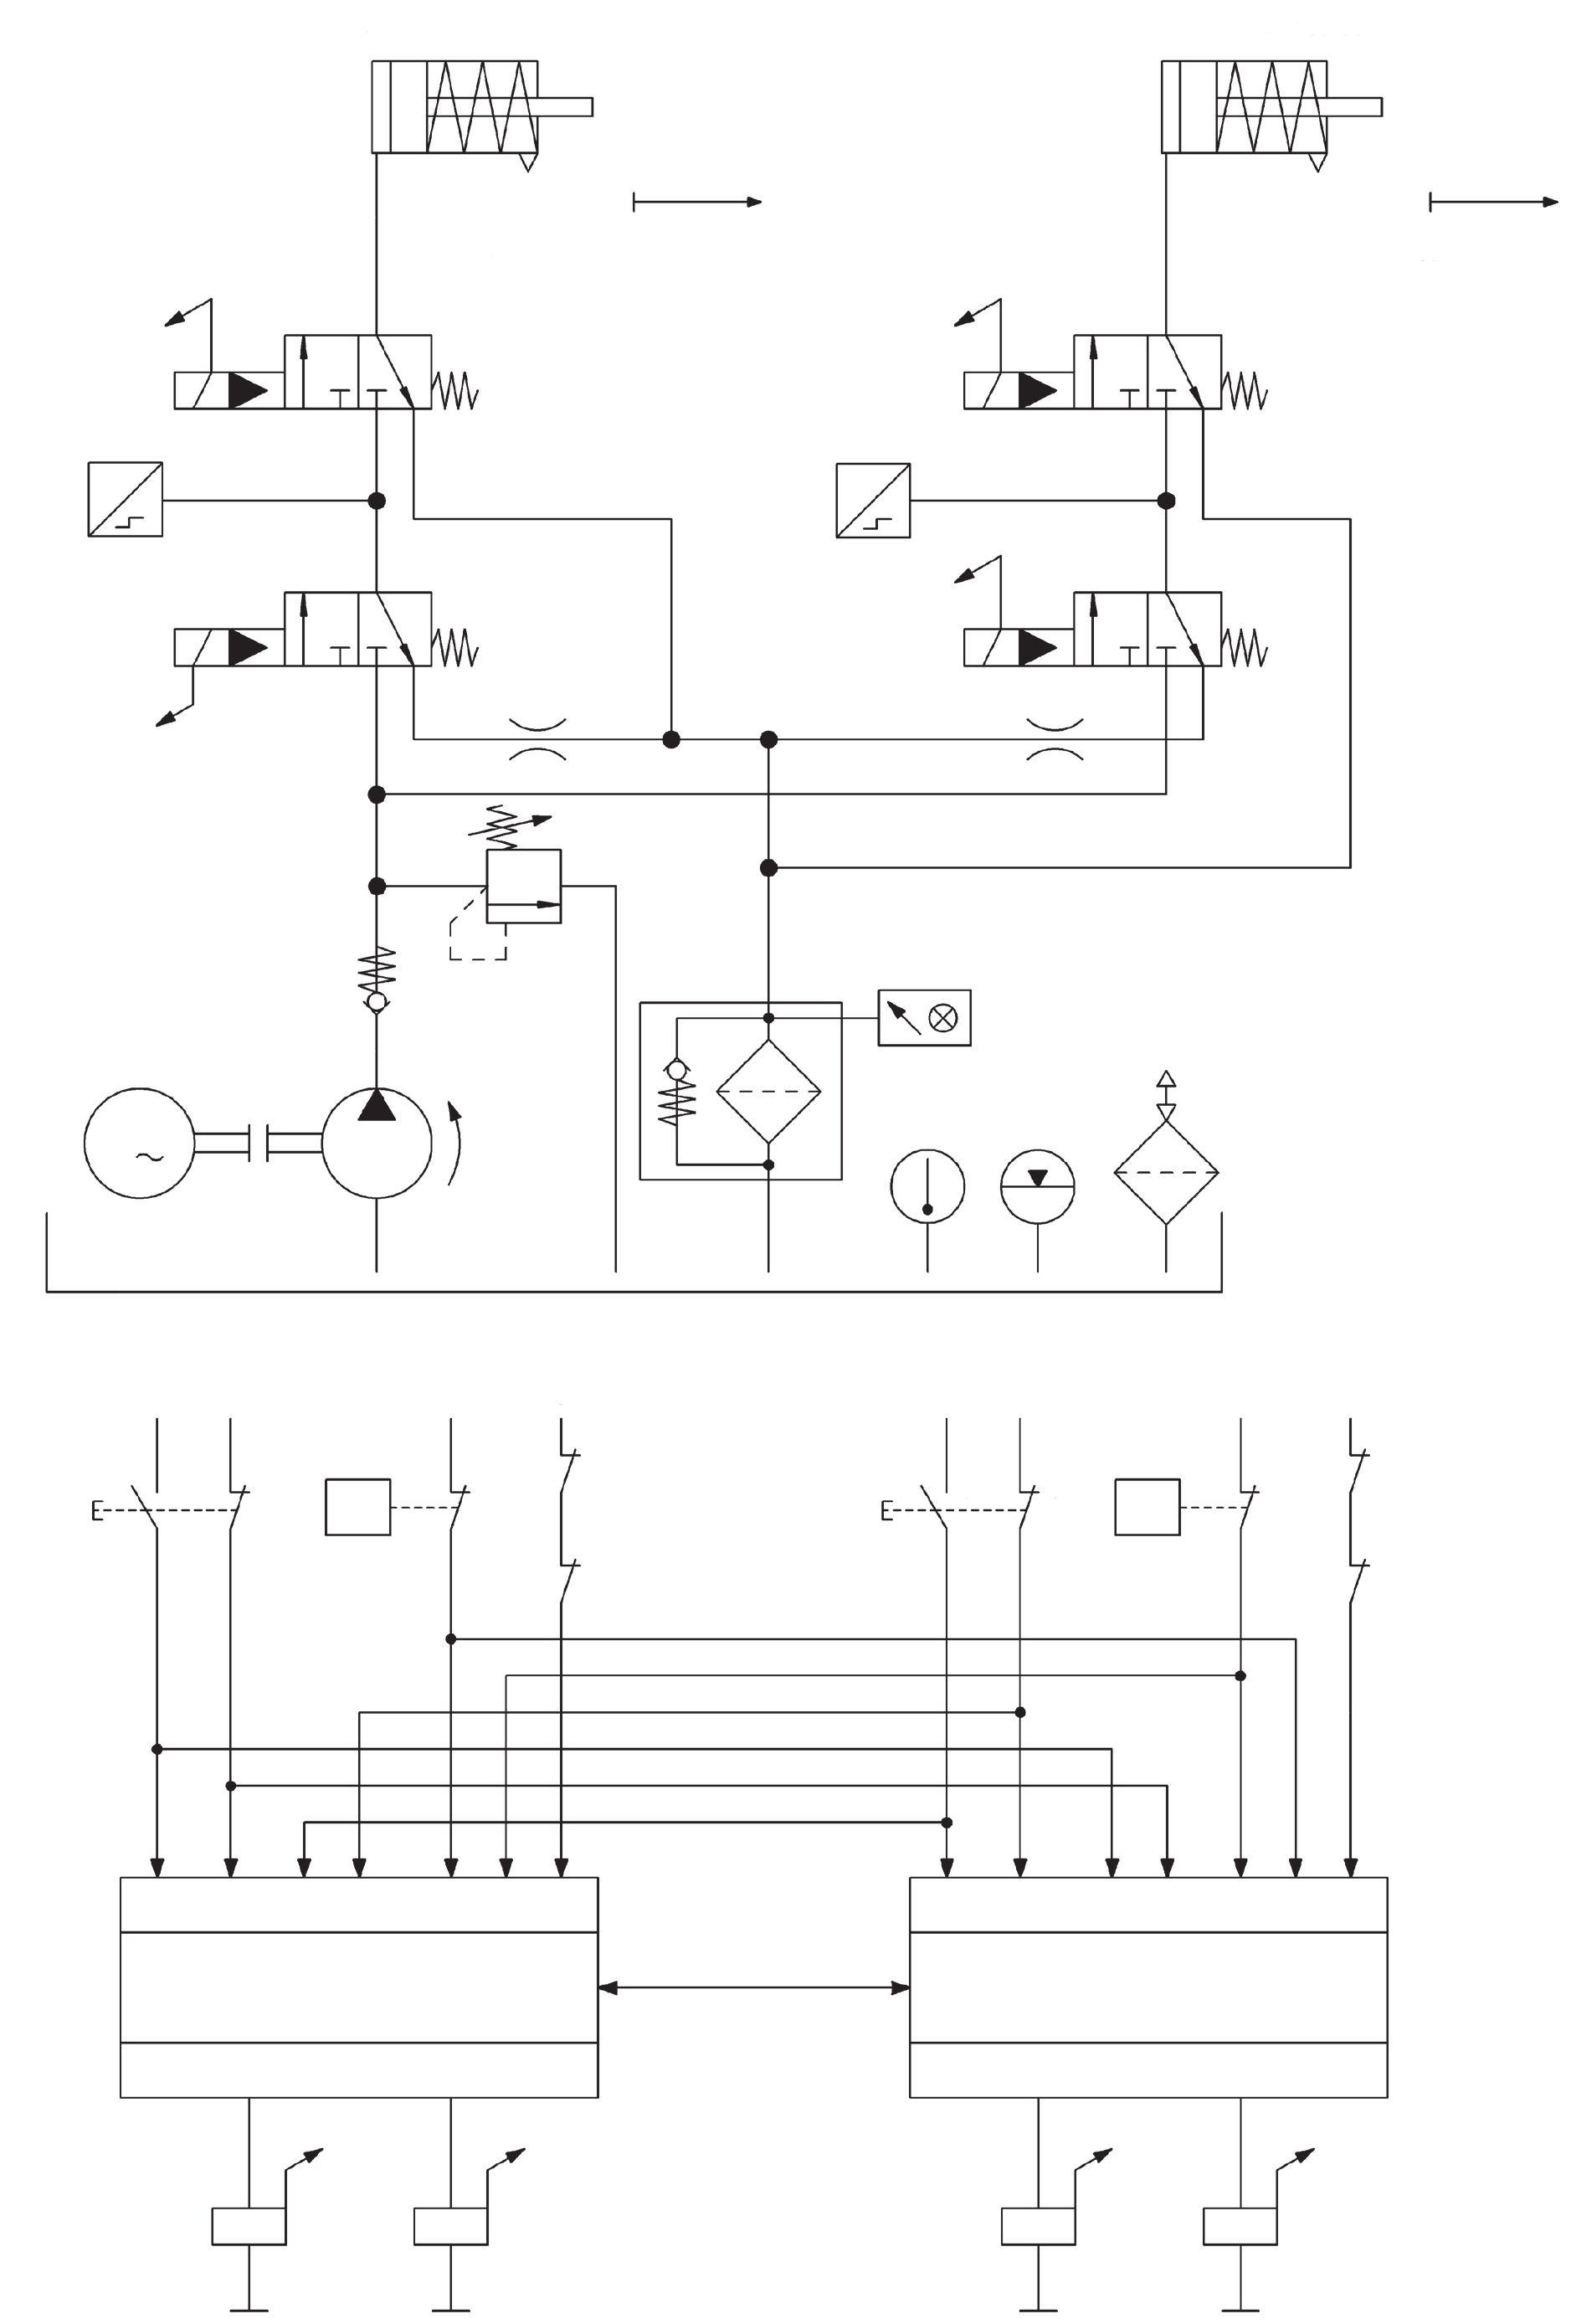
\includegraphics[width=15.740cm, height=23.289cm]{img06-15.png}};

% --- scritte: diciture tradotte e sigle dei componenti ---
\node[grande] at (153.06,661.35) {Azionamento della lama};
\node[grande] at (385.72,661.35) {Barra di pressione};
\node[media] at (121.89,641.37) {1A};
\node[media] at (348.32,641.37) {2A};
\node[grande, align=center] at (225.54,596.72) {Movimento\\pericoloso};
\node[grande, align=center] at (446.75,596.72) {Movimento\\pericoloso};
\node[media] at (290.19,578.77) {K4};
\node[media] at (64.14,577.83) {K3};
\node[media] at (62.25,561.48) {1V4};
\node[media] at (288.83,560.08) {2V2};
\node[media] at (54.92,533.22) {P};
\node[media] at (270.05,533.22) {P};
\node[media] at (39.65,530.42) {1S3};
\node[media] at (251.99,528.78) {2S1};
\node[media] at (290.24,504.02) {K6};
\node[media] at (63.93,486.97) {1V3};
\node[media] at (288.66,486.97) {2V1};
\node[media] at (177.03,471.55) {1V5};
\node[media] at (326.88,471.55) {2V3};
\node[media] at (61.86,463.85) {K5};
\node[media] at (152.71,424.61) {1V2};
\node[media] at (117.51,391.91) {1V1};
\node[media] at (213.40,389.80) {1Z2};
\node[media] at (347.14,364.27) {1Z1};
\node[media] at (62.67,350.80) {M};
\node[media] at (288.65,347.29) {1S1};
\node[media] at (319.81,347.29) {1S2};
\node[media] at (39.70,344.56) {1M};
\node[media] at (164.79,344.56) {1P};
\node[media] at (58.55,340.52) {3};
\node[media] at (68.19,273.17) {+};
\node[media] at (88.51,273.17) {+};
\node[media] at (151.73,273.17) {+};
\node[media] at (183.81,273.17) {+};
\node[media] at (294.06,273.17) {+};
\node[media] at (315.39,273.17) {+};
\node[media] at (378.29,273.17) {+};
\node[media] at (409.43,273.17) {+};
\node[media] at (125.76,254.49) {1S3};
\node[media] at (351.97,254.48) {2S1};
\node[media] at (175.14,250.75) {K5};
\node[media] at (402.66,249.50) {K3};
\node[piccola] at (76.90,245.46) {13};
\node[piccola] at (305.03,245.15) {13};
\node[piccola] at (100.28,244.84) {21};
\node[piccola] at (328.41,244.53) {21};
\node[grande] at (125.81,240.14) {P\textgreater{}};
\node[grande] at (351.92,240.14) {P\textgreater{}};
\node[media] at (40.98,239.54) {S1};
\node[media] at (268.03,239.54) {S2};
\node[piccola] at (77.07,233.63) {14};
\node[piccola] at (100.86,233.63) {22};
\node[piccola] at (305.19,233.32) {14};
\node[piccola] at (328.98,233.32) {22};
\node[media] at (175.54,219.61) {K6};
\node[media] at (402.86,218.35) {K4};
\node[media] at (45.39,127.10) {K1};
\node[media] at (272.53,127.10) {K2};
\node[media] at (348.66,125.24) {Ingresso};
\node[media] at (116.32,125.24) {Ingresso};
\node[grande] at (352.38,104.97) {ASIC};
\node[grande] at (121.69,103.73) {Microcontrollore};
\node[media, align=center] at (239.52,102.35) {Sincronizzazione e\\scambio di dati};
\node[media] at (119.66,78.83) {Uscita};
\node[media] at (351.99,78.83) {Uscita};
\node[media] at (115.49,61.40) {1V4};
\node[media] at (174.54,61.39) {2V2};
\node[media] at (342.68,61.39) {1V3};
\node[media] at (399.69,61.39) {2V1};
\node[media] at (134.62,34.61) {K4};
\node[media] at (74.35,34.60) {K3};
\node[media] at (302.22,34.60) {K5};
\node[media] at (360.56,34.60) {K6};

% --- cornice esterna ---
\draw[draw=black, line width=0.75pt] (0.37,0.37) rectangle (497.93,677.81);

\end{tikzpicture}
}
        \captionof{figure}{Schema di principio dell'azionamento elettronico di una lama idraulica e di una barra di pressione idraulica (componenti essenziali).}
        \label{fig:06-15}
    \end{minipage}
\end{center}

\textbf{Descrizione funzionale}
\begin{itemize}
    \item l'azionamento degli attuatori S1 e S2 del comando bimanuale avvia i movimenti pericolosi (ciclo di lavorazione) della barra di pressione e della lama. Qualora uno dei due attuatori del comando bimanuale venga rilasciato durante questo ciclo, oppure si verifichi una variazione di segnale nel sistema periferico della macchina non attesa dal sistema di comando, il ciclo viene interrotto e la macchina assume lo stato sicuro;
    \item la pressione degli attuatori S1 e S2 fa sì che i fronti di salita dei segnali vengano inviati ai due canali di elaborazione K1 (microcontrollore) e K2 (ASIC). A condizione che tali segnali soddisfino i requisiti di simultaneità (500 ms) secondo la pertinente norma EN 574, i due canali di elaborazione impostano le uscite (relè a contattore K3-K6) per una richiesta di taglio valida;
    \item i due canali di elaborazione operano in modo sincrono e valutano inoltre reciprocamente gli stati intermedi interni delle operazioni cicliche di elaborazione dei segnali. Scostamenti dagli stati intermedi definiti causano l'arresto della macchina. Un canale di elaborazione è costituito da un microcontrollore (K1), l'altro da un ASIC (K2). K1 e K2 eseguono autotest in background durante il funzionamento;
    \item i guasti negli attuatori S1/S2 e nei relè a contattore K3-K6 (con contatti di riscontro meccanicamente collegati) sono rilevati mediante monitoraggio incrociato nei canali di elaborazione;
    \item il guasto delle valvole 1V3/1V4 e 2V1/2V2 è rilevato mediante i pressostati 1S3 e 2S1.
    \item il guasto delle valvole, o il blocco in posizione aperta di 1V4 o 2V2, è rilevato tramite una forte riduzione della velocità di ritorno dei cilindri idraulici. Questa situazione può essere rilevata anche dal sistema di comando mediante un'opportuna interpretazione dei segnali di pressione (durata della caduta di pressione);
    \item il guasto delle valvole, o il blocco in posizione aperta di 1V3 o 2V1, è rilevato direttamente mediante il monitoraggio della variazione di segnale dei pressostati 1S3 e 2S1: qualora una valvola resti bloccata, viene segnalata una pressione anche quando non dovrebbe essere presente alcuna pressione;
    \item tutti gli stati della macchina sono monitorati da entrambi i canali di elaborazione. La natura ciclica dell'operazione di taglio fa sì che tutti gli stati del sistema vengano percorsi ciclicamente, consentendo così il rilevamento dei guasti."
\end{itemize}

\subsection{Schema a blocchi legato alla sicurezza}
\label{subsec:06-5-4}
La descrizione della struttura circuitale, unitamente allo schema elettrico e, ove applicabile, ad altri documenti descrittivi (specifica esaustiva), consente di determinare una categoria di comando e di ricondurre il circuito effettivo a uno schema a blocchi legato alla sicurezza in forma astratta (Figura 6.16, pag. 78). Da questo esempio risulta rapidamente evidente che la funzione di sicurezza è eseguita in modalità a due canali. Possono pertanto essere prese in considerazione la categoria 3 o la categoria 4. Le misure di test di alta qualità, mediante le quali possono essere controllate anche le combinazioni di guasti, fanno propendere per la categoria 4. Ciò viene dimostrato esplicitamente dalla fase di verifica nel Capitolo 7, così come la verifica dei requisiti quantitativi relativi a MTTF\textsubscript{D}, DC\textsubscript{avg} e CCF (vedere oltre). Le spiegazioni fornite ai punti 6.2.8 e 6.2.9 sono utili per la realizzazione dello schema a blocchi legato alla sicurezza. Una procedura collaudata consiste nel seguire il percorso del segnale, iniziando dal lato attuatore, ponendosi la domanda: "Come viene azionato/impedito il movimento pericoloso?", per poi seguire la logica a ritroso fino ai sensori. Il SISTEMA Cookbook 1 [34] descrive questo passaggio, "Dallo schema circuitale al Performance Level", in maggiore dettaglio.

Si noti, in questo esempio, che gli attuatori S1 e S2 non sono ridondanti tra loro, anche se a prima vista potrebbero sembrarlo, poiché ciascun pulsante protegge indipendentemente una delle mani dell'utilizzatore. La ridondanza inizia piuttosto all'interno di ciascun pulsante, con l'impiego di combinazioni di contatti elettrici di apertura/di chiusura. Ciascun canale di comando monitora entrambe le mani/attuatori interpretando almeno un contatto elettrico di commutazione in ciascun attuatore. Lo schema a blocchi legato alla sicurezza contiene pertanto, in ciascun canale, un contatto di chiusura, ad es. S1/13-14, e un contatto di apertura, ad es. S2/21-22. Lo schema a blocchi legato alla sicurezza differisce sotto questo aspetto in modo sostanziale dallo schema elettrico funzionale.

In determinate circostanze, la realizzazione effettiva della funzione di sicurezza può comportare restrizioni o raccomandazioni per l'applicazione. Ad esempio, l'efficacia del rilevamento dei guasti attraverso il processo di lavorazione è per definizione strettamente legata all'applicazione.

\subsection{Grandezze di ingresso per la valutazione quantitativa del PL raggiunto}
\label{subsec:06-5-5}
A questo punto sono disponibili tutte le informazioni di base per la valutazione del PL raggiunto. Conoscendo la Categoria e lo schema a blocchi relativo alla sicurezza, è possibile determinare innanzitutto l'MTTF\textsubscript{D} e la DC dei singoli blocchi e valutare, per le ridondanze presenti, le misure contro i guasti di causa comune (CCF).

\textbf{Calcolo della probabilità di guasto}:
\begin{itemize}
    \item MTTF\textsubscript{D}: con 240 giorni lavorativi all'anno, 8 ore lavorative al giorno e un tempo di ciclo di 80 secondi, n\textsubscript{op} risulta pari a 86.400 cicli all'anno. Per S1 e S2 e per K3-K6, un valore di B\textsubscript{10D} pari a 2.000.000 di cicli [M] produce un MTTF\textsubscript{D} di 232 anni. Per il solo microcontrollore viene determinato un MTTF\textsubscript{D} di 1.142 anni [D]. Lo stesso valore viene sostituito anche per l'ASIC [D]. Insieme alla relativa disposizione circuitale, ciò dà luogo, in entrambi i casi, a un MTTF\textsubscript{D} di 806 anni per i blocchi K1 e K2. Il fabbricante indica un MTTF\textsubscript{D} di 150 anni [M] per ciascuna delle valvole idrauliche 1V3, 1V4, 2V1 e 2V2. Questi valori producono un MTTF\textsubscript{D} per ciascun canale pari a 31,4 anni ("alto");
    \item DC\textsubscript{avg}: conformemente all'Allegato E della EN ISO 13849-1, i valori di DC ottenuti sono: per S1/S2: 99\% (monitoraggio incrociato dei segnali di ingresso senza test dinamico con variazione frequente del segnale); per K1/K2: 90\% (autotest tramite software e monitoraggio incrociato); per K3-K6: 99\% (monitoraggio diretto mediante contatti meccanicamente collegati); per 1V3/2V1: 99\% (monitoraggio indiretto tramite il sensore di pressione); e per 1V4/2V2: 99\% (monitoraggio indiretto tramite la funzione e la misura di una variazione della durata della caduta di pressione). Questi valori danno luogo a una DC\textsubscript{avg} del 98,6\% ("alta");
    \item misure adeguate contro i guasti per causa comune (65 punti): separazione (15), protezione da sovratensione ecc. (15) e condizioni ambientali (25 + 10);
    \item la combinazione degli elementi di comando soddisfa la categoria 4 con un MTTF\textsubscript{D} per canale alto (31,4 anni) e una DC\textsubscript{avg} del 98,6\%, entro la fascia di tolleranza "alta". Ne risulta una probabilità media di guasto pericoloso di 9,7 10\textsuperscript{-8} all'ora. Ciò soddisfa il PL e;
\end{itemize}

Per chiarire il calcolo dell'MTTF\textsubscript{D} si considera anzitutto il blocco "K1": sebbene lo schema concettuale (Figura 6.15) mostri soltanto il microcontrollore, questo blocco comprende ulteriori elementi necessari per la funzionalità pratica (ad es. l'oscillatore al quarzo). Devono essere considerati tutti gli elementi il cui guasto pericoloso potrebbe impedire l'esecuzione della funzione di sicurezza nel canale interessato. Ciò comprende generalmente tutti gli elementi presenti nel percorso del segnale critici per la sicurezza, ad esempio per il disaccoppiamento, il riscontro, la protezione CEM o la protezione contro la sovratensione. Questi elementi sono generalmente necessari per la realizzazione dei principi di sicurezza di base e ben collaudati o per il raggiungimento della DC. La Figura B.2 (vedere pag. 253) illustra questo approccio con riferimento a un ulteriore esempio semplice. 

Il metodo del conteggio dei componenti (parts count) mostrato nella Tabella~\ref{tab:06-8} è adatto come semplice metodo tabellare per determinare l'MTTF\textsubscript{D} del blocco a partire dall'MTTF\textsubscript{D} dei singoli elementi. (Per confronto, la Figura B.3 a pag. 255 mostra la procedura per un'analisi dei modi di guasto e dei loro effetti.)

I tassi di guasto degli elementi indicati nella seconda colonna sono stati determinati mediante la banca dati SN 29500 [49], come indicato dal codice [D] alla voce "calcolo della probabilità di guasto" (vedere punto 7.6). La convalida è descritta più in dettaglio nel seguito di questo esempio, al punto 7.6. Poiché elementi identici possono comparire più volte (terza colonna), il tasso di guasto complessivo per ciascun tipo di elemento viene calcolato e indicato nella quarta colonna. L'approssimazione generale secondo cui soltanto la metà dei guasti è pericolosa produce il valore dimezzato riportato nella colonna 5. Infine, una semplice sommatoria produce il tasso complessivo di guasti pericolosi per il blocco K1. La colonna 6 mostra i corrispondenti valori di MTTF\textsubscript{D} in anni, ricavati come reciproci dei tassi di guasto pericoloso (dalla colonna 5, dopo la conversione da ore ad anni). Questo valore è arrotondato a 806 anni per il blocco K1. Poiché la banca dati impiegata indica tassi di guasto identici per il microcontrollore e per l'ASIC, e il circuito è analogo, il valore di MTTF\textsubscript{D} di 806 anni si applica anche al blocco K2.

% Tabella non fluttuante (minipage + \captionof): a fine capitolo un float
% finirebbe da solo su una pagina a parte.
%
% La quinta colonna e' riquadrata in grassetto perche' e' quella che alimenta
% il totale: filetti verticali spessi nel preambolo (!{\vrule width 1.2pt}) e
% tratti orizzontali spessi sopra e sotto con \cmidrule[1.2pt]{5-5}.
% La barra del totale e' una seconda tabularx con le stesse larghezze di
% colonna, cosi' i due valori restano incolonnati con quelli di sopra.
\begin{center}
    \begin{minipage}{\textwidth}
    \captionsetup{hypcap=false}
    \definecolor{tabblue}{RGB}{31,73,125}
    \setlength{\tabcolsep}{3pt}
    \renewcommand{\arraystretch}{1.25}
    \setstretch{1}
    \footnotesize
    % frecce del riepilogo
    \newcommand{\frecciagiu}{\tikz[baseline=-0.4ex]{\fill
        (-0.09,0.30) -- (0.09,0.30) -- (0.09,0.06) -- (0.20,0.06) --
        (0,-0.16) -- (-0.20,0.06) -- (-0.09,0.06) -- cycle;}}
    \newcommand{\frecciadx}{\tikz[baseline=-0.5ex]{\fill
        (-0.30,-0.09) -- (-0.30,0.09) -- (-0.06,0.09) -- (-0.06,0.20) --
        (0.16,0) -- (-0.06,-0.20) -- (-0.06,-0.09) -- cycle;}}
    \captionof{table}{Metodo del conteggio dei componenti (\textit{parts count}) per il blocco "microcontrollore" K1, sulla base dei tassi di guasto $\lambda$ tratti dalla raccolta di dati SN~29500~\cite{sn29500} (espressi in FIT, ossia $10^{-9}$ all'ora).}
    \label{tab:06-8}

    \begin{tabularx}{\textwidth}{%
        |>{\raggedright\arraybackslash}p{5.7cm}%
        |>{\centering\arraybackslash}p{2.3cm}%
        |>{\centering\arraybackslash}p{1.3cm}%
        |>{\centering\arraybackslash}p{1.9cm}%
        !{\vrule width 1.2pt}>{\centering\arraybackslash}p{2.0cm}%
        !{\vrule width 1.2pt}|C|}
        \hline
        \cmidrule[1.2pt]{5-5}
        \rowcolor{tabblue}
        \textcolor{white}{\textbf{Componente}} &
        \textcolor{white}{\textbf{Tasso di guasto $\lambda$ in FIT secondo la SN~29500}} &
        \textcolor{white}{\textbf{Numero}} &
        \textcolor{white}{\textbf{Tasso di guasto totale $\lambda$ in FIT}} &
        \textcolor{white}{\textbf{Tasso totale di guasti pericolosi $\lambda_{\mathrm{D}}$ in FIT}} &
        \textcolor{white}{\textbf{\textit{MTTF}\textsubscript{D} in anni come reciproco di $\lambda_{\mathrm{D}}$}} \\
        \hline
        Resistore a film metallico        & 0,2 & 7 & 1,4 & 0,7 & 163.079 \\
        \hline
        \rowcolor{black!8}
        Condensatore, non alimentato      & 1   & 4 & 4   & 2   & 57.078 \\
        \hline
        Diodo per impieghi generali       & 1   & 3 & 3   & 1,5 & 76.104 \\
        \hline
        \rowcolor{black!8}
        Optoaccoppiatore, uscita bipolare & 15  & 2 & 30  & 15  & 7.610 \\
        \hline
        Microcontrollore                  & 200 & 1 & 200 & 100 & 1.142 \\
        \hline
        \rowcolor{black!8}
        Oscillatore al quarzo             & 15  & 1 & 15  & 7,5 & 15.221 \\
        \hline
        Transistor bipolare, bassa potenza & 20 & 1 & 20  & 10  & 11.416 \\
        \hline
        \rowcolor{black!8}
        Relè con incapsulamento in plastica & 10 & 1 & 10 & 5   & 22.831 \\
        \hline
        \cmidrule[1.2pt]{5-5}
    \end{tabularx}

    % freccia verso il basso, incolonnata sotto la quinta colonna
    \vspace{2pt}
    \begin{tabularx}{\textwidth}{%
        @{}p{5.7cm}@{}p{2.3cm}@{}p{1.3cm}@{}p{1.9cm}%
        @{}>{\centering\arraybackslash}p{2.0cm}@{}X@{}}
        & & & & \frecciagiu & \\
    \end{tabularx}

    \vspace{2pt}
    \begin{tabularx}{\textwidth}{%
        |>{\raggedright\arraybackslash}p{5.7cm}%
        |>{\centering\arraybackslash}p{2.3cm}%
        |>{\centering\arraybackslash}p{1.3cm}%
        |>{\centering\arraybackslash}p{1.9cm}%
        |>{\centering\arraybackslash}p{2.0cm}|C|}
        \hline
        \rowcolor{black!8}
        \multicolumn{4}{|>{\raggedright\arraybackslash}p{11.62cm}|}{Totale per il blocco "microcontrollore" K1} &
        \fbox{141,7 FIT} &
        \frecciadx\enspace\fbox{806 anni} \\
        \hline
    \end{tabularx}
    \end{minipage}
\end{center}

Per i blocchi S1/S2 e K3-K6 sono utilizzati i dati dei fabbricanti ("[M]"). Poiché i dati di affidabilità sono disponibili soltanto per S1/S2 nel loro complesso (meccanismo di azionamento e contatto di apertura e di chiusura), questi valori possono essere utilizzati come stima a favore della sicurezza per ciascuno dei canali, anche se in ciascun canale vengono considerati soltanto i contatti di chiusura (ad es. S1/13-14) oppure i contatti di apertura (ad es. S2/21-22), oltre al meccanismo di azionamento. I valori di B\textsubscript{10D} assunti vengono convertiti in valori di MTTF\textsubscript{D} mediante le formule già note dall'Allegato D:

\begin{equation}
    n_{\mathrm{op}}
    = \frac{d_{\mathrm{op}} \cdot h_{\mathrm{op}}}{t_{\mathrm{ciclo}}} \cdot 3{.}600\,\frac{\mathrm{s}}{\mathrm{h}}
    = \frac{240\ \text{giorni/anno} \cdot 8\ \text{h/giorno}}{80\ \text{s/ciclo}} \cdot 3{.}600\,\frac{\mathrm{s}}{\mathrm{h}}
    = 86{.}400\,\frac{\text{cicli}}{\text{anno}}
    \label{eq:06-06}
\end{equation}

\begin{equation}
    \textit{MTTF}_{\mathrm{D}}
    = \frac{B_{\mathrm{10D}}}{0{,}1 \cdot n_{\mathrm{op}}}
    = \frac{2{.}000{.}000\ \text{cicli}}{0{,}1 \cdot 86{.}400\ \text{cicli/anno}}
    = 231{,}5\ \text{anni}
    \label{eq:06-07}
\end{equation}

La durata di funzionamento dei componenti elettromeccanici è limitata al valore T\textsubscript{10D} (tempo dopo il quale il 10\% dei componenti oggetto dell'analisi si è guastato in modo pericoloso). Poiché tuttavia, in questo caso, il valore di T\textsubscript{10D} è superiore al tempo di missione assunto di 20 anni, esso non è rilevante ai fini dell'ulteriore analisi. Dato che in:

\begin{equation}
    T_{\mathrm{10D}}
    = \frac{B_{\mathrm{10D}}}{n_{\mathrm{op}}}
    = \frac{2{.}000{.}000\ \text{cicli}}{86{.}400\ \text{cicli/anno}}
    = 23{,}2\ \text{anni}
    \label{eq:06-08}
\end{equation}

Il fabbricante indica inoltre un MTTF\textsubscript{D} di 150 anni [M] per ciascuna delle valvole idrauliche 1V3, 1V4, 2V1 e 2V2. Conformemente al punto 6.2.13, il totale per un canale (S1, S2, K1, K3, K4, 1V4, 2V2) produce un MTTF\textsubscript{D} di 31,4 anni, ossia "alto"."

% a corpo pieno la formula riempie tutta la riga e spinge il numero a capo:
% \small la stringe quel tanto che basta perche (9) resti in linea
{\small
\begin{equation}
    \frac{1}{\textit{MTTF}_{\mathrm{D}}}
    = \frac{1}{232\ \text{anni}} + \frac{1}{232\ \text{anni}} + \frac{1}{806\ \text{anni}}
    + \frac{1}{232\ \text{anni}} + \frac{1}{232\ \text{anni}} + \frac{1}{150\ \text{anni}}
    + \frac{1}{150\ \text{anni}}
    = \frac{1}{31{,}4\ \text{anni}}
    \label{eq:06-09}
\end{equation}
}

Poiché il secondo canale presenta lo stesso MTTF\textsubscript{D}, non è necessaria la simmetrizzazione, come sarebbe altrimenti il caso. Anche la convalida dei valori di DC assunti è descritta più in dettaglio nel Capitolo 7. Autotest di alta qualità, ad esempio, vengono eseguiti per K1 e K2 mediante software e monitoraggio incrociato, comprese le misure speciali per la memoria variante e invariante e per l'unità di elaborazione, richieste per i sistemi a microprocessore. Nel complesso, per la SRP/CS si ottiene, conformemente al punto 6.2.14, una DC\textsubscript{avg} del 98,6\%. Sfruttando la tolleranza del 5\%, questo valore rientra nella fascia "alta".


% formula molto larga (14 frazioni): \small la fa stare nella giustezza
{\small
\begin{equation}
    \textit{DC}_{\mathrm{avg}}
    = \frac{2 \cdot \left(
        \dfrac{99\%}{232\ \text{anni}} + \dfrac{99\%}{232\ \text{anni}}
        + \dfrac{90\%}{806\ \text{anni}} + \dfrac{99\%}{232\ \text{anni}}
        + \dfrac{99\%}{232\ \text{anni}} + \dfrac{99\%}{150\ \text{anni}}
        + \dfrac{99\%}{150\ \text{anni}}
      \right)}
      {2 \cdot \left(
        \dfrac{1}{232\ \text{anni}} + \dfrac{1}{232\ \text{anni}}
        + \dfrac{1}{806\ \text{anni}} + \dfrac{1}{232\ \text{anni}}
        + \dfrac{1}{232\ \text{anni}} + \dfrac{1}{150\ \text{anni}}
        + \dfrac{1}{150\ \text{anni}}
      \right)}
    = 98{,}6\%
    \label{eq:06-10}
\end{equation}
}

Le misure contro i guasti per causa comune (CCF) indicate nel riquadro grigio a pag. 78 sono in gran parte autoesplicative. La convalida è comunque descritta più in dettaglio nel Capitolo 7. Inoltre, la misura "diversità" e la misura "impiego di componenti ben collaudati" trovano applicazione rispettivamente nel sottosistema elettrico e in quello idraulico (vedere Allegato F). Con la soddisfazione dei requisiti relativi ai CCF, una DC\textsubscript{avg} "alta" e un MTTF\textsubscript{D} "alto", risultano soddisfatti anche i requisiti quantitativi della categoria 4.

\subsection{Diversi approcci per il calcolo del PL}
\label{subsec:06-5-6}
La determinazione del PL sulla base degli aspetti quantificabili è ormai quasi completa a questo punto. I risultati relativi a categoria, DC\textsubscript{avg} e MTTF\textsubscript{D} possono essere utilizzati per una conferma grafica, mediante il diagramma a barre, del fatto che venga raggiunto il PL e (vedere Figura~\ref{fig:06-17}). I valori tabellari dell'Allegato K della norma, o il calcolatore a disco PLC dell'IFA [16] basato su di essi, forniscono il seguente risultato:
\begin{center}
    \begin{minipage}{\textwidth}
    \captionsetup{hypcap=false}
    \centering
    \definecolor{tabblue}{RGB}{31,73,125}
    \setlength{\tabcolsep}{4pt}
    \renewcommand{\arraystretch}{1.25}
    \setstretch{1}
    \captionof{table}{Riepilogo delle grandezze di ingresso e del PL raggiunto dal sistema di comando della taglierina a ghigliottina.}
    \label{tab:06-9}

    \begin{tabular}{%
        |>{\centering\arraybackslash}p{2.1cm}%
        |>{\centering\arraybackslash}p{1.4cm}%
        |>{\centering\arraybackslash}p{2.0cm}%
        |>{\centering\arraybackslash}p{3.2cm}%
        |>{\centering\arraybackslash}p{4.4cm}|}
        \hline
        \rowcolor{tabblue}
        \textcolor{white}{\textbf{Categoria}} &
        \textcolor{white}{\textbf{CCF}} &
        \textcolor{white}{\textbf{\textit{DC}\textsubscript{avg}}} &
        \textcolor{white}{\textbf{\textit{MTTF}\textsubscript{D}}} &
        \textcolor{white}{\textbf{\textit{PFH}\textsubscript{D}}}
        \tabularnewline
        \hline
        4 & OK & "alta" &
        "alto" \newline (arrotondato per difetto: 30~anni) &
        \cellcolor{black!8} $9{,}5 \cdot 10^{-8}$ all'ora \newline (PL~e)
        \tabularnewline
        \hline
    \end{tabular}
    \end{minipage}
\end{center}

% La minipage tiene insieme disegno e didascalia (figura non fluttuante)
\begin{center}
    \begin{minipage}{\textwidth}
        \centering
        \captionsetup{hypcap=false}
        \resizebox{0.92\textwidth}{!}{%==============================================================
%  Figura 6.17 - Determinazione del PL mediante il diagramma
%  a barre / il disco di calcolo PLC
%  Adattamento in italiano della Figura 6.17 dell'IFA Report 2/2017
%  (pagina 80 di rep0217e.pdf)
%
%  Il diagramma a barre riusa il sistema di riferimento della
%  Figura 6.10 (immagini/fig06-10.tex): stesse coordinate in punti
%  PostScript dell'originale, unita' della tikzpicture x=y=0.042cm,
%  origine nell'angolo in basso a sinistra del riquadro del grafico.
%  Il riquadro sovrapposto riproduce il disco PLC dell'IFA; i marchi
%  (IFA, ZVEI, VDMA) sono resi in forma testuale semplificata.
%==============================================================
\begin{tikzpicture}[
  x=0.042cm, y=0.042cm,
  font=\small,
  cornice/.style={draw=black, line width=0.9pt},
  riquadro/.style={draw=black, line width=1.06pt},
  griglia/.style={draw=black, line width=1.06pt,
                  dash pattern=on 4.24pt off 2.12pt},
  tacca/.style={draw=black, line width=1.06pt},
  separatore/.style={draw=black, line width=0.8pt},
  contorno/.style={draw=black, line width=0.8pt},
  puntini/.style={draw=black, line width=0.52pt, line cap=butt,
                  dash pattern=on 0.53pt off 1.05pt},
  tratti/.style={draw=black, line width=0.52pt},
  etichetta/.style={draw=black, fill=black!15, line width=1.06pt,
                    rounded corners=2.9pt, inner sep=0pt, align=center},
  evidenza/.style={draw=black!55, fill=white, line width=1.2pt,
                   rounded corners=3.5pt, inner sep=0pt, align=center},
  fumetto/.style={draw=black, fill=white, line width=1.1pt,
                  inner sep=2pt, align=center},
  passo/.style={circle, fill=black!42, inner sep=0pt, align=center},
  frecciagrigia/.style={draw=black!42, line width=7pt,
                        -{Triangle[length=10pt, width=13pt]}},
  tratteggiata/.style={draw=black, line width=1.7pt,
                       dash pattern=on 6pt off 4pt,
                       -{Triangle[length=8pt, width=8pt]}}
]

\setstretch{1}

% --- riempimenti delle barre ------------------------------------------
\def\riempipuntini#1#2#3#4{%
  \begin{scope}
    \clip (#1,#2) rectangle (#3,#4);
    \foreach \k in {0,...,20}{%
      \draw[puntini] (#1,{#4-1.1-2.2155*\k}) -- (#3,{#4-1.1-2.2155*\k});}
  \end{scope}}
\def\riempitratti#1#2#3#4{%
  \begin{scope}
    \clip (#1,#2) rectangle (#3,#4);
    \foreach \k in {0,...,34}{%
      \draw[tratti] (#1,{#2-(#4-#2)+3.13*\k})
        -- ++({(#3-#1)+(#4-#2)},{(#3-#1)+(#4-#2)});}
  \end{scope}}
\def\barrabassa#1#2#3#4{%
  \fill[white] (#1,#2) rectangle (#3,#4);
  \riempipuntini{#1}{#2}{#3}{#4}
  \draw[contorno] (#1,#2) rectangle (#3,#4);}
\def\barramedia#1#2#3#4{%
  \fill[white] (#1,#2) rectangle (#3,#4);
  \riempitratti{#1}{#2}{#3}{#4}
  \draw[contorno] (#1,#2) rectangle (#3,#4);}
\def\barraalta#1#2#3#4{%
  \fill[black] (#1,#2) rectangle (#3,#4);
  \draw[contorno] (#1,#2) rectangle (#3,#4);}

% --- colonna delle PFHD a sinistra --------------------------------------
\draw[black!15, line width=6.62pt] (-38.64,211.73) -- (-38.64,0.44);

\node[etichetta, minimum width=1.4423cm, minimum height=1.1726cm]
  at (-38.81,218.58) {\textit{PFH}$_{\mathrm{D}}$\\(1/h)};

\foreach \yv/\testo in {175.89/{$10^{-4}$}, 140.50/{$10^{-5}$},
                        105.15/{$3\cdot 10^{-6}$}, 70.05/{$10^{-6}$},
                        34.87/{$10^{-7}$}, 0/{$10^{-8}$}}{%
  \draw[tacca] (-23.86,\yv) -- (-2.81,\yv);
  \node[etichetta, minimum width=1.4423cm, minimum height=0.5586cm]
    at (-38.81,\yv) {\testo};}

% --- asse dei PL ---------------------------------------------------------
\node at (-10.4,217.7) {PL};
\draw[draw=black, line width=1.06pt, -{Triangle[length=11pt,width=6pt]}]
  (0.03,-41.87) -- (0.03,208.69);
\foreach \yv/\pl in {158.2/a, 122.8/b, 87.6/c, 52.5/d}
  \node at (-9.0,\yv) {\pl};
% il PL raggiunto nell'esempio e' evidenziato
\node[evidenza, minimum width=0.55cm, minimum height=0.55cm]
  at (-9.0,17.4) {e};

% --- riquadro del grafico e griglia --------------------------------------
\draw[riquadro] (0,0) rectangle (342.01,175.89);
\foreach \yv in {140.50, 105.15, 70.05, 34.87}
  \draw[griglia] (0.05,\yv) -- (342.03,\yv);

% --- barre ----------------------------------------------------------------
% Cat. B, DCavg = nessuna
\barrabassa{13.85}{143.10}{35.23}{160.84}
\barramedia{13.85}{111.48}{35.23}{143.10}
% Cat. 1, DCavg = nessuna
\barraalta{62.57}{74.80}{83.95}{111.08}
% Cat. 2, DCavg = bassa
\barrabassa{111.69}{130.62}{133.07}{155.26}
\barramedia{111.69}{92.81}{133.07}{130.62}
\barraalta{111.69}{60.92}{133.07}{92.81}
% Cat. 2, DCavg = media
\barrabassa{160.52}{120.54}{181.89}{151.25}
\barramedia{160.52}{76.21}{181.89}{120.54}
\barraalta{160.52}{48.10}{181.89}{76.21}
% Cat. 3, DCavg = bassa
\barrabassa{209.34}{106.01}{230.72}{144.25}
\barramedia{209.34}{64.80}{230.72}{106.01}
\barraalta{209.34}{34.98}{230.72}{64.80}
% Cat. 3, DCavg = media
\barrabassa{258.11}{79.85}{279.48}{125.46}
\barramedia{258.11}{50.07}{279.48}{79.85}
\barraalta{258.11}{22.31}{279.48}{50.07}
% Cat. 4, DCavg = alta
\barraalta{306.93}{13.89}{328.31}{34.23}

% --- lettura del risultato: barra Cat. 4 -> asse dei PL --------------------
\draw[black!42, line width=3.2pt] (317.6,13.0) -- (317.6,-3.0);
\draw[draw=black!42, line width=4pt, dash pattern=on 13pt off 9pt,
      -{Triangle[length=9pt, width=11pt]}] (335,34.87) -- (4,34.87);

% --- intestazioni delle colonne ------------------------------------------
\foreach \xv in {48.79, 97.59, 146.34, 195.12, 243.93, 292.69}
  \draw[separatore] (\xv,6.96) -- (\xv,-41.88);

\foreach \xc/\cat/\dc in {24.4/B/nessuna, 73.2/1/nessuna, 122.0/2/bassa,
                          170.7/2/media, 219.5/3/bassa, 268.3/3/media,
                          317.4/4/alta}{%
  \node at (\xc,-10.1) {Cat.~\cat};
  \node[align=center] at (\xc,-31.5)
    {\textit{DC}$_{\mathrm{avg}}$\,=\\\dc};}
% la colonna dell'esempio e' evidenziata
\draw[draw=black!55, line width=1.2pt, rounded corners=3.5pt]
  (296.5,-40.5) rectangle (338.5,-2.5);

%==========================================================================
%  Riquadro sovrapposto: il disco di calcolo PLC dell'IFA
%==========================================================================
\definecolor{plca}{RGB}{214,0,110}
\definecolor{plcb}{RGB}{247,168,196}
\definecolor{plcc}{RGB}{243,146,0}
\definecolor{plcd}{RGB}{255,242,175}
\definecolor{plce}{RGB}{214,237,214}
\definecolor{ifablu}{RGB}{0,86,160}
\definecolor{vdmablu}{RGB}{0,51,102}
\definecolor{zveiblu}{RGB}{0,75,141}

\fill[white] (93.7,65.2) rectangle (329.6,239.1);
\draw[riquadro] (93.7,65.2) rectangle (329.6,239.1);

% --- corpo del disco -------------------------------------------------------
\fill[black!5] (218,152) circle (67);
\draw[draw=black!45, line width=0.8pt, dash pattern=on 3pt off 2pt]
  (218,152) circle (69.5);

% --- finestra dei valori di PFHD ------------------------------------------
\foreach \k/\etichetta/\valore/\colore in {%
  0/{Cat.~1}/{3,80}/plcb,
  1/{Cat.~2, DC bassa}/{2,06}/plcc,
  2/{Cat.~2, DC media}/{1,21}/plcc,
  3/{Cat.~3, DC bassa}/{6,94}/plcd,
  4/{Cat.~3, DC media}/{2,65}/plcd,
  5/{Cat.~4, DC alta}/{9,54}/plce}{%
  \node[anchor=east, font=\tiny] at (213,{214.5-4.9*\k}) {\etichetta};
  \fill[\colore] (214.5,{212.1-4.9*\k}) rectangle (223.5,{216.9-4.9*\k});
  \draw[draw=black!55, line width=0.3pt]
    (214.5,{212.1-4.9*\k}) rectangle (223.5,{216.9-4.9*\k});
  \node[font=\tiny] at (219,{214.5-4.9*\k}) {\valore};}
% riga selezionata nell'esempio
\draw[draw=black, line width=0.7pt] (186.5,187.2) rectangle (213.6,192.0);

\node[anchor=west, font=\tiny\bfseries, align=left] at (225,206.5)
  {probabilità media\\di guasto\\pericoloso\\per ora};

% --- scritte del disco ------------------------------------------------------
\node[font=\footnotesize] at (222,183.5)
  {Performance Level Calculator$^{\copyright}$\,--\,PLC};
\node[font=\tiny] at (222,177)
  {per informazioni e applicazioni vedere www.dguv.de/ifa/13849};
\node[font=\footnotesize] at (222,169.5) {per EN ISO 13849-1};

% perno centrale del disco
\fill[black] (218,152.5) circle (1.6);
\draw[black, line width=0.7pt] (214.5,152.5) -- (221.5,152.5);
\draw[black, line width=0.7pt] (218,149) -- (218,156);

% --- marchio IFA -------------------------------------------------------------
\begin{scope}[shift={(176,141)}]
  \fill[ifablu] (0,0) circle (3.4);
  \fill[white] (-3.6,-0.5) rectangle (3.6,1.3);
\end{scope}
\node[anchor=west, font=\large\bfseries, text=black!75] at (181,140.5) {IFA};
\node[anchor=west, font=\tiny, align=left, text=black!75] at (176,133)
  {Institut für Arbeitsschutz der\\Deutschen Gesetzlichen Unfallversicherung};

% --- legenda dei PL sul disco --------------------------------------------------
\node[anchor=west, font=\tiny] at (256,163.5) {PL:};
\foreach \k/\pl/\colore/\esp in {0/a/plca/{-5}, 1/b/plcb/{-6}, 2/c/plcc/{-6},
                                 3/d/plcd/{-7}, 4/e/plce/{-8}}{%
  \node[font=\tiny] at (257.5,{156-8.2*\k}) {\pl};
  \fill[\colore] (261,{153.3-8.2*\k}) rectangle (267.5,{158.7-8.2*\k});
  \node[anchor=west, font=\tiny] at (270,{156-8.2*\k}) {$\times\,10^{\esp}$};}

% --- marchi ZVEI e VDMA ---------------------------------------------------------
\node[anchor=west, font=\footnotesize\bfseries, text=zveiblu] at (183,108) {ZVEI:};
\draw[red!70!black, line width=0.6pt] (183,104.6) -- (200,104.6);
\node[anchor=west, font=\small\bfseries, text=vdmablu] at (233,108) {VDMA};
\foreach \r in {4.6,6.2,7.8}
  \draw[orange, line width=0.9pt] (231,108) ++(120:\r) arc (120:210:\r);

% --- finestra dell'MTTFD --------------------------------------------------------
\node[font=\footnotesize] at (213,91.5) {\textit{MTTF}$_{\mathrm{D}}$};
\node[font=\tiny] at (211,85.5) {[anni]};
\fill[white] (222.5,78.5) rectangle (233.5,84);
\draw[draw=black!70, line width=0.5pt] (222.5,78.5) rectangle (233.5,84);
\node[font=\tiny] at (228,81.2) {30};

%==========================================================================
%  Passi di utilizzo del disco (annotazioni)
%==========================================================================
% 1. impostare l'MTTFD di ciascun canale e la barra Cat. 4, DC alta
\draw[frecciagrigia] (293,214) .. controls (307,200) and (309,175) .. (306,146);
\node[passo, minimum size=0.94cm, font=\large] at (304.5,195) {1.};

\draw[frecciagrigia, line width=6pt] (243,82) -- (235,81.2);
\node[passo, minimum size=0.94cm, font=\large] at (252.5,81.2) {1.};

\node[fumetto, font=\large, minimum width=1.2cm] at (281,92) {30};

% 2. lettura del risultato nelle finestre del disco
\draw[frecciagrigia, line width=6pt] (188,180) -- (199,187);
\node[passo, minimum size=0.84cm, font=\large] at (182,175.5) {2.};

\node[fumetto, font=\large, minimum height=0.44cm] at (152,226) {Cat.~4, DC alta};
\draw[black, line width=0.7pt] (196,221.5) -- (189,192.2);

\draw[tratteggiata] (212,188) -- (159,173);
\node[fumetto, font=\large, minimum width=1.15cm] at (145,173) {9,54};
\node[font=\large] at (142,161) {$\cdot\,10^{-8}$};

\draw[tratteggiata] (259,123) -- (158,137);
\node[fumetto, font=\large, minimum width=1.15cm] at (143,137) {PL~e};

% --- cornice esterna --------------------------------------------------------
\draw[cornice] (-66.19,242.74) rectangle (347.91,-48);

\end{tikzpicture}
}
        \captionof{figure}{Determinazione del PL mediante il diagramma a barre / il disco di calcolo.}
        \label{fig:06-17}
    \end{minipage}
\end{center}

Il software SISTEMA (vedere Allegato H), disponibile gratuitamente presso l'IFA, risulta molto più agevole per la gestione, la documentazione e il calcolo di tutti i risultati intermedi. Tutti i requisiti quantitativi per la determinazione del PL descritti finora possono essere gestiti facilmente con questo software, e tutti i calcoli, compresa la determinazione matematica del PL, sono automatizzati. Come opzione speciale è possibile utilizzare per il calcolo i valori esatti di DC\textsubscript{avg} e MTTF\textsubscript{D}. Per la DC\textsubscript{avg} viene impiegato ai fini del calcolo il valore esatto (in questo caso più sfavorevole) del 98,6\%, anziché sfruttare la tolleranza del 5\% per una DC\textsubscript{avg} "alta" e sostituire un valore arrotondato del 99\% (per le tolleranze relative a DC e MTTF\textsubscript{D}, cfr. la Nota 2 delle Tabelle 4 e 5 della norma). Lo scendere al di sotto della soglia del 99\% per la categoria 4, pur restando entro la fascia di tolleranza, fa tuttavia scattare in SISTEMA un messaggio di avvertimento. L'impiego, ai fini del calcolo, del valore preciso di MTTF\textsubscript{D} pari a 31,4 anni produce un risultato paragonabile a quello ottenuto con il valore arrotondato di 30 anni per l'MTTF\textsubscript{D} "alto". Il risultato è una probabilità media di guasto pericoloso per ora pari a 9,7 · 10\textsuperscript{-8} all'ora (vedere Figura~\ref{fig:06-18}).

% Schermata del software SISTEMA (figura non fluttuante)
\begin{center}
    \begin{minipage}{\textwidth}
        \centering
        \captionsetup{hypcap=false}
        \fbox{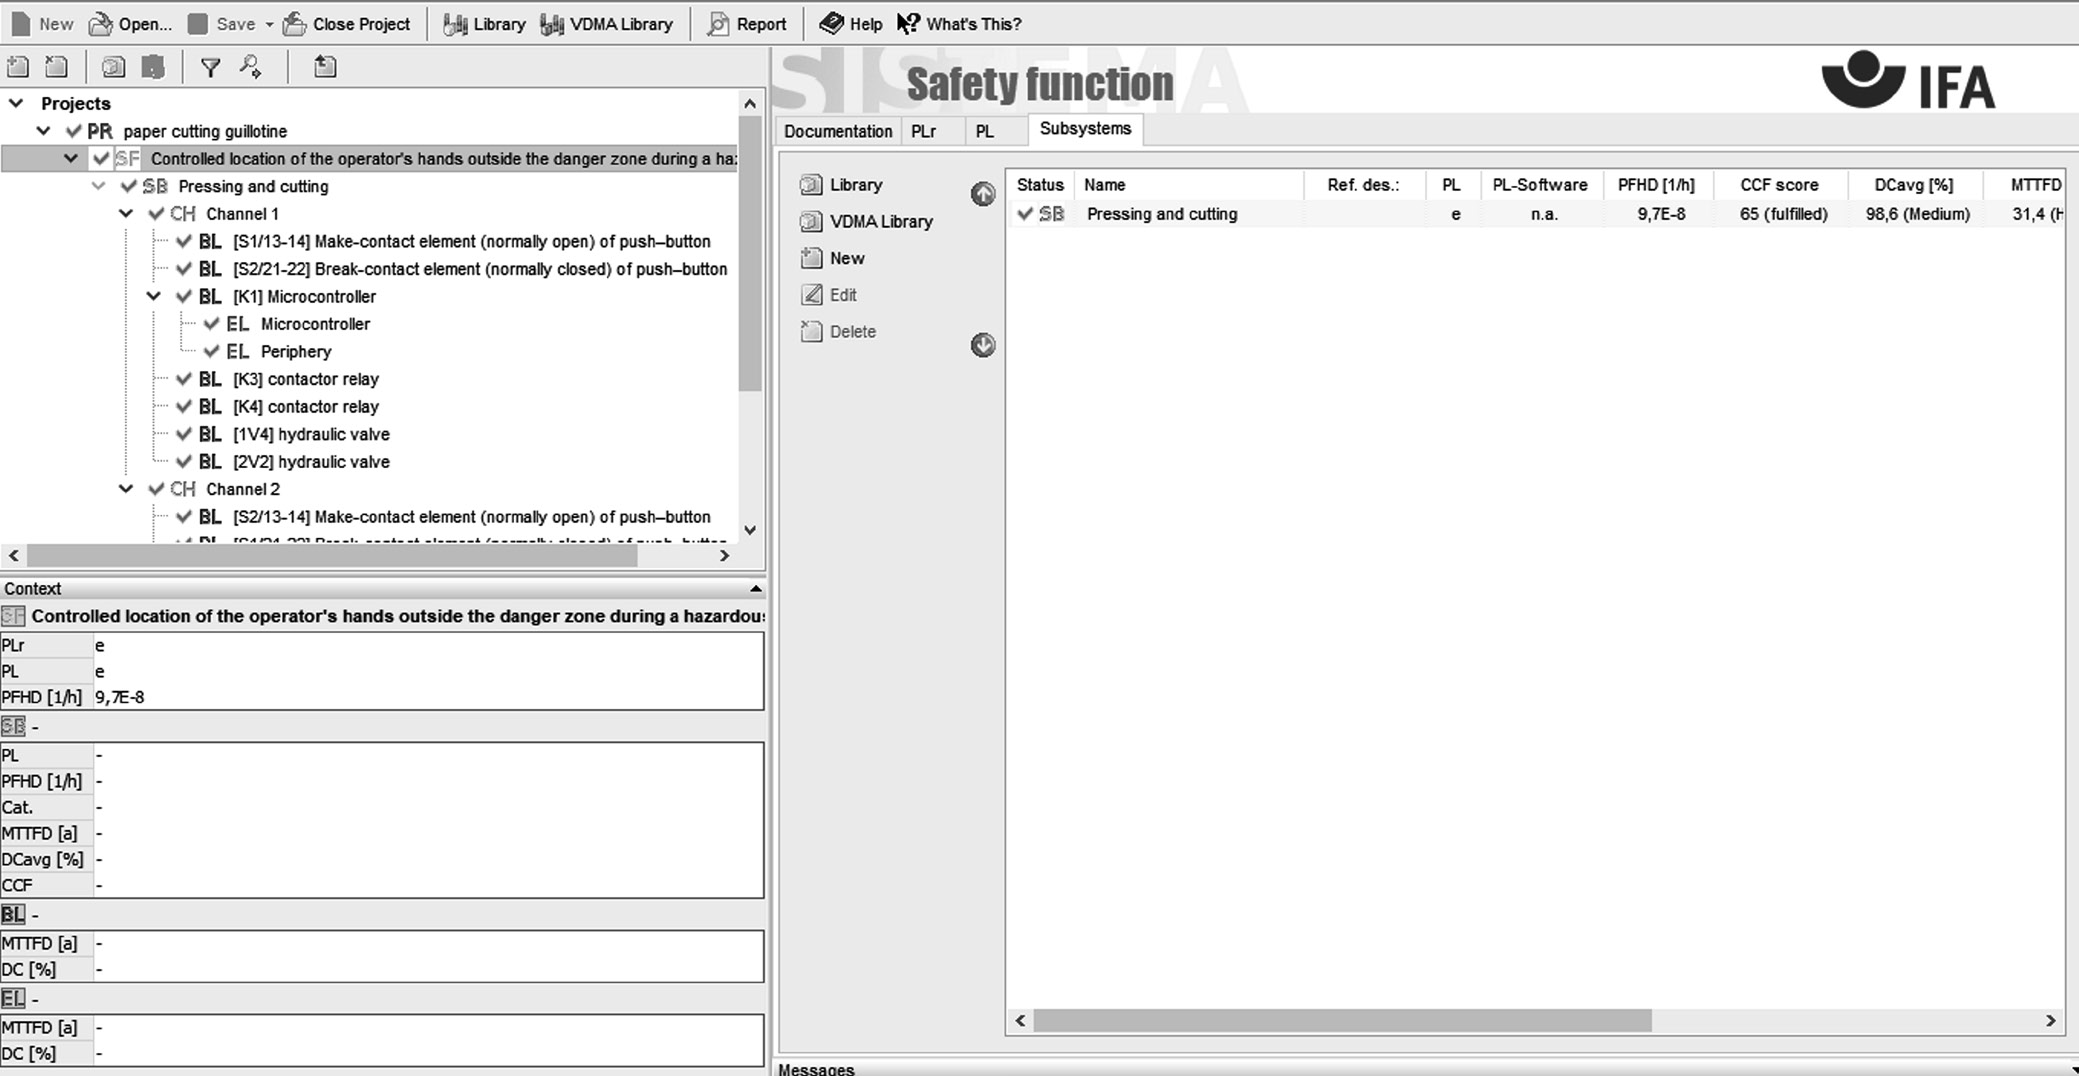
\includegraphics[width=0.95\textwidth]{img06-18.png}}
        \captionof{figure}{Determinazione del PL mediante SISTEMA.}
        \label{fig:06-18}
    \end{minipage}
\end{center}

A questo punto segue la valutazione degli aspetti qualitativi non quantificabili per la determinazione del PL, in primo luogo per quanto riguarda i guasti sistematici.

\subsection{Guasti sistematici}
\label{subsec:06-5-7}
Con il suo approccio orientato alla diversità per il comando logico, la configurazione selezionata del sistema di comando impiega una misura altamente efficace contro l'influenza dei guasti sistematici. Nel corso della realizzazione sono naturalmente richieste ulteriori misure, ad esempio al fine di controllare gli effetti di un'interruzione della tensione, delle fluttuazioni di tensione, della sovratensione e della sottotensione. Alcune delle misure necessarie sono già evidenti nella configurazione selezionata. Tra queste:
\begin{itemize}
    \item impiego del principio della corrente di riposo: ciò garantisce che lo stato diseccitato non possa dare origine a un segnale di azionamento (ad es. in caso di rottura di un conduttore);
    \item rilevamento dei guasti mediante test automatici: in questo caso vengono eseguiti test - differenti tra i due canali - in grado di rilevare i guasti in una fase precoce e di avviare lo stato sicuro indipendentemente dal rispettivo canale adiacente.
    \item test mediante hardware ridondante: la diversità di progettazione fornisce un controllo aggiuntivo dei guasti causati da influenze ambientali che hanno effetti diversi sui diversi canali.
    \item impiego di relè a contattore con contatti meccanicamente collegati: il rilevamento dello stato di contatti idonei consente di rilevare guasti pericolosi dei relè a contattore e, in alcuni casi, di altri componenti circuitali.
    \item monitoraggio della sequenza del programma: l'ASIC, ad esempio, viene utilizzato per monitorare la sequenza del programma del canale a microcontrollore.
\end{itemize}

L'attenzione del lettore è richiamata in particolare su due aspetti relativi ai guasti sistematici, il primo riguardante l'applicazione, il secondo il processo di progettazione:
\begin{itemize}
    \item durante la progettazione del sistema idraulico per le taglierine a ghigliottina per carta, occorre tenere conto della presenza di polvere di carta. La contaminazione del fluido idraulico con polvere di carta può ad esempio compromettere la funzione sicura di una taglierina a ghigliottina per carta. Per questo motivo, particolare attenzione deve essere prestata a un'efficace filtrazione del fluido in pressione. Deve inoltre essere impedita la penetrazione di polvere di carta nel sistema idraulico dall'esterno, ad esempio mediante filtri di sfiato del serbatoio e anelli raschiatori sugli steli dei cilindri.
    \item misure di evitamento dei guasti durante lo sviluppo dell'ASIC, conformemente al ciclo di vita di sviluppo dell'ASIC previsto dalla IEC 61508-2. Questa norma prevede, per lo sviluppo di un ASIC, un modello a V analogo a quello già noto dallo sviluppo del software.
\end{itemize}

\subsection{Aspetti ergonomici}
\label{subsec:06-5-8}
In questo esempio esiste un'interfaccia legata alla sicurezza tra l'utilizzatore e il sistema di comando: il dispositivo di comando bimanuale (THC), con gli attuatori S1 e S2. Al riguardo devono essere considerati determinati aspetti ergonomici, al fine di evitare che qualsiasi persona sia messa in pericolo, direttamente o nel tempo a causa di sollecitazioni dannose, durante l'uso previsto e l'uso scorretto ragionevolmente prevedibile della macchina. Per la maggior parte delle macchine, queste interfacce utente possono essere verificate mediante la lista di controllo per la progettazione ergonomica delle macchine, pubblicazioni informative DGUV 209-068 e 209-069 [30]. Gli aspetti da osservare in questo contesto comprendono i seguenti:
\begin{itemize}
    \item altezza e orientamento degli attuatori rispetto all'operatore
    \item spazio per le gambe e area di raggiungimento durante il funzionamento, normalmente in posizione eretta
    \item disposizione adattata al compito operativo e buona accessibilità al di fuori della zona pericolosa
    \item facilità di osservazione del processo di taglio dalla postazione del THC
    \item dimensioni minime e forma degli attuatori (progettazione ergonomica in considerazione dei requisiti della EN 574)
    \item azionamento agevole con forze contenute, ma con misure progettuali per la prevenzione dell'azionamento involontario
    \item costruzione robusta dei pulsanti, e marcatura e colorazione idonee
    \item THC progettato per impedire la neutralizzazione e quindi l'elusione del posizionamento controllato delle mani dell'operatore
\end{itemize}

\subsection{Requisiti relativi al software, in particolare al SRESW}
\label{subsec:06-5-9}
La seguente descrizione riguarda un'implementazione modello di firmware legato alla sicurezza per il microcontrollore K1. Il software è software embedded (SRESW) per il quale il PL\textsubscript{r} è e. Grazie all'approccio orientato alla diversità del comando logico - il secondo canale assume la forma di un ASIC - i requisiti possono essere ridimensionati conformemente alla nota del punto 4.6.2 della norma: "Quando si impiega la diversità nella specifica, nella progettazione e nella codifica, per i due canali utilizzati in SRP/CS di categoria 3 o 4, il PL\textsubscript{r} e può essere raggiunto con le misure sopra indicate previste per un PL\textsubscript{r} di c o d."

Il processo di progettazione del firmware si basa sul modello a V della Figura 6.11 ed è integrato nel sistema di gestione della qualità certificato del fabbricante. A partire dalla specifica dell'intero sistema di comando legato alla sicurezza, viene anzitutto redatta la specifica dei requisiti di sicurezza del software per il firmware (safety related software requirements specification). Questo documento descrive il contributo fornito dal firmware alle funzioni di sicurezza della macchina, i tempi di risposta richiesti per K1, le reazioni ai guasti rilevati, le interfacce verso altri sottosistemi, le dipendenze dai modi di funzionamento, ecc. Vengono inoltre definite tutte le misure di evitamento dei guasti richieste dal punto 6.3.2 della norma per PL c o d. La specifica viene quindi sottoposta a revisione, ad esempio da parte del responsabile del progetto di sicurezza, con eventuali modifiche apportate se del caso. Una volta approvata la specifica, può avere inizio la progettazione del sistema.

Architettura del software: sul microcontrollore non è installato un sistema operativo; vengono invece definiti una serie di task che, controllati da una semplice gestione dei task, sono eseguiti tramite interrupt temporizzato a intervalli definiti. Alcuni task a bassa priorità sono riservati alle funzioni standard della taglierina a ghigliottina per carta, mentre i task ad alta priorità sono eseguiti dalle funzioni legate alla sicurezza sopra specificate. Il determinismo di queste chiamate ai task è necessario per l'elevata sincronicità richiesta tra i due canali e per i brevi tempi di risposta. Gli autotest ciclici per il controllo dei guasti casuali dell'hardware vengono eseguiti durante i tempi morti (idle) dei task.

La progettazione dell'architettura software e dei moduli e delle funzioni software necessari per la realizzazione del software sopra descritto sono riepilogati in un ulteriore documento, la specifica tecnica per la progettazione del sistema e dei moduli. Ai fini dell'evitamento dei guasti lungo l'intero ciclo di vita, sono particolarmente importanti un'idonea modularizzazione e, in questo caso, anche una netta separazione del SRESW dal software non legato alla sicurezza. Ove necessario per ragioni di chiarezza, la struttura e il flusso del software sono rappresentati mediante diagrammi. Vengono inoltre stabiliti ulteriori requisiti relativi al linguaggio di programmazione da utilizzare, in questo caso l'ANSI C con estensioni linguistiche specifiche del compilatore, e agli strumenti di sviluppo, ad es. compilatore, gestione delle versioni, gestione della configurazione; tutti impiegati con successo da molti anni. Sono inoltre specificate le linee guida di programmazione e i metodi per l'analisi statica basata su strumenti (tools) per la verifica della codifica. In questo documento è definita anche la pianificazione dei test di modulo e di integrazione. A seguito di un'ulteriore revisione, ad esempio da parte del responsabile dello sviluppo software, la specifica tecnica viene approvata come specifica per la codifica. Questa revisione verifica anche se i requisiti della specifica del software siano stati soddisfatti.

Ha ora inizio la codifica vera e propria, in conformità alle linee guida di programmazione. Oltre a regole per una migliore leggibilità del codice, le disposizioni delle linee guida di programmazione specificano, ad esempio, vincoli sull'uso di costrutti linguistici critici. L'osservanza delle linee guida di programmazione durante la codifica è garantita in-process mediante l'impiego di strumenti idonei. Per la verifica semantica (del contenuto) del codice finito rispetto alla specifica tecnica, il programmatore conduce un walk-through con i colleghi, in cui vengono contestualmente analizzati l'esecuzione del programma e il flusso di dati dei segnali critici.

Vengono eseguiti i consueti test di modulo per verificare le funzioni e le interfacce, in primo luogo per la correttezza e in secondo luogo per la conformità alla progettazione del modulo. Segue quindi l'integrazione del software e i test insieme all'hardware del microcontrollore K1. K1 viene quindi collegato al canale ASIC K2 per testare la sincronizzazione, lo scambio di dati e il rilevamento dei guasti dei due canali in combinazione. Tutti i test sono documentati.

Questo test di integrazione può rivelare che le prestazioni del microcontrollore non sono buone come precedentemente ipotizzato. In tal caso, l'architettura software - in particolare la pianificazione dei task e l'assegnazione delle funzioni a essi - deve essere modificata. Ciò non comporterebbe modifiche alla specifica dei requisiti di sicurezza del software; la progettazione del sistema e dei moduli, tuttavia, dovrebbe essere adattata e sottoposta nuovamente a revisione, al fine di garantire la conformità alla specifica. Questo è un esempio di come le modifiche tecniche che si rendono necessarie durante lo sviluppo possano comportare la ripetizione del modello a V, affinché le modifiche siano realizzate in conformità ai requisiti di assicurazione qualità (QA). Il codice per tali modifiche dovrebbe essere scritto, e sia il test di modulo sia il test di integrazione dovrebbero essere ripetuti.

Per il caso in cui il firmware debba essere modificato dopo che il primo lotto di produzione sia già stato spedito, misure idonee, quali un'analisi d'impatto delle modifiche e opportune attività di sviluppo conformi al modello a V, dovrebbero essere definite nell'ambito dell'organizzazione stessa dello sviluppo

\subsection{SRP/CS in combinazione}
\label{subsec:06-5-10}
Poiché l'intera SRP/CS è strutturata in modo continuo (end-to-end) in un'unica categoria e non vengono combinati sottosistemi, non è richiesta la relativa analisi secondo il punto 6.4. È tuttavia evidente che i diversi componenti e le diverse tecnologie devono essere compatibili alle loro interfacce. Gli aspetti di validazione relativi all'integrazione sono trattati nel Capitolo 7

\subsection{Ulteriori dettagli}
\label{subsec:06-5-11}
Anche in questo dettagliato esempio circuitale, numerosi aspetti progettuali legati alla sicurezza possono essere soltanto accennati. Viene pertanto fornito qui, come nella maggior parte degli esempi circuitali che seguono, un rimando a riferimenti utili contenenti ulteriori spiegazioni e indicazioni relative a requisiti aggiuntivi.

\textbf{Riferimenti}:
\begin{itemize}
    \item EN 1010-3: Sicurezza del macchinario - Requisiti di sicurezza per la progettazione e la costruzione di macchine per la stampa e la trasformazione della carta - Parte 3: Macchine da taglio (2002) +A1 (2009)
    \item IEC 61508-2: Sicurezza funzionale dei sistemi elettrici/elettronici/elettronici programmabili legati alla sicurezza - Parte 2: Requisiti per i sistemi elettrici/elettronici/elettronici programmabili legati alla sicurezza (2010)
    \item EN 574: Sicurezza del macchinario - Dispositivi di comando bimanuale - Aspetti funzionali; principi di progettazione (1996) +A1 (2008) (in via di sostituzione con la EN ISO 13851:2019)
\end{itemize}

%==============================================================
%  CAPITOLO 7
%==============================================================
\chapter{Verifica e validazione}
\label{cap:07}

Breve introduzione al capitolo: oggetto, obiettivi e collegamento
con i capitoli precedenti.

%--------------------------------------------------------------
\section{Prima sezione}
\label{sec:07-1}

Testo della sezione.

\subsection{Sottosezione}
\label{subsec:07-1-1}

Testo della sottosezione.

%--------------------------------------------------------------
\section{Seconda sezione}
\label{sec:07-2}

Testo della sezione.

%--------------------------------------------------------------
\section{Conclusioni del capitolo}
\label{sec:07-3}

Sintesi dei contenuti e rimandi al capitolo successivo.

%==============================================================
%  CAPITOLO 8
%==============================================================
\chapter{Esempi di circuiti SRP/C}
\label{cap:08}
Questo report inizia trattando la progettazione di sistemi di controllo sicuri in termini generali. I paragrafi~\ref{sec:05-7}, 6.5 e 7.6 illustrano quindi, con riferimento all'esempio di una ghigliottina per il taglio della carta, come possono essere implementati i metodi per la progettazione di sistemi di controllo sicuri. I metodi per la determinazione del PL sono descritti passo-passo qui e nella norma EN ISO 13849-1; tuttavia, alcuni di questi passaggi, come la derivazione del diagramma a blocchi relativo alla sicurezza dallo schema elettrico, richiedono una certa pratica. Il manuale di SISTEMA~\cite{cookbook1} fornisce indicazioni su come derivare il diagramma a blocchi relativo alla sicurezza e il file SISTEMA dallo schema elettrico.

Tuttavia, a causa della varietà delle possibili funzioni di sicurezza e della loro implementazione, i singoli passaggi non si prestano a una descrizione generica. Per questo motivo, questo capitolo presenterà ora la valutazione di numerosi esempi di circuiti che implementano le funzioni di sicurezza in varie categorie e livelli di prestazione e mediante diverse tecnologie. Negli esempi di circuiti, il concetto di sistema di controllo generalmente comprende solo le parti dei sistemi di controllo relative alla sicurezza. Gli esempi sono limitati agli aspetti essenziali e servono quindi principalmente a illustrare la metodologia. Nella loro selezione è stata data importanza a un ampio spettro di tecnologie e possibili applicazioni. I lettori che hanno familiarità con il report del 1997~\cite{en954-1} sulle Categorie per i sistemi di controllo relativi alla sicurezza secondo la norma EN 954-1 riconosceranno alcuni degli esempi, ai quali è stato aggiunto, ad esempio, il calcolo della probabilità di guasto. Rispetto al Rapporto BGIA 2/2008e~\cite{bgiareport2-2008}, alcuni esempi non più aggiornati sono stati eliminati; è stato tuttavia aggiunto un nuovo esempio. Gli esempi rappresentano un'interpretazione delle Categorie e sono stati compilati dagli autori sulla base di molti anni di esperienza con i sistemi di controllo delle macchine relativi alla sicurezza e del lavoro svolto in comitati di normazione nazionali ed europei. Gli esempi servono a fornire ai progettisti una guida efficace per i loro sviluppi.

Poiché gli esempi sono stati creati da autori diversi, esiste inevitabilmente una certa variabilità, ad esempio nella presentazione dei dettagli o nel ragionamento alla base di alcuni dati numerici. Tutti i calcoli per gli esempi di circuito sono stati eseguiti con l'ausilio della versione 2.0 dell'applicazione software SISTEMA (vedere Allegato H), la versione disponibile al momento della produzione di questo rapporto. Ulteriori esempi di circuito, inclusi i file SISTEMA, sono descritti anche nel rapporto IFA 4/2018e, "Controlli di azionamento sicuri con inverter di frequenza"~\cite{werner2019}.

La descrizione di ciascun esempio è strutturata come segue:
\begin{itemize}
    \item funzione di sicurezza
    \item descrizione funzionale
    \item caratteristiche progettuali
    \item osservazioni
    \item calcolo della probabilità di guasto
    \item riferimenti più dettagliati
\end{itemize}

Alla voce "funzione di sicurezza" viene indicato il nome della funzione di sicurezza, unitamente agli eventi che la attivano e alle risposte di sicurezza richieste.

La "descrizione funzionale" descrive le funzioni essenziali legate alla sicurezza, sulla base di uno schema concettuale. Viene spiegato il comportamento in caso di guasto, e vengono indicate le misure per il rilevamento dei guasti.
Le caratteristiche particolari della progettazione dell'esempio in questione, quali l'applicazione di principi di sicurezza ben collaudati e l'impiego di componenti ben collaudati, sono elencate alla voce "caratteristiche progettuali".

Gli schemi circuitali sono schemi concettuali, limitati esclusivamente alla rappresentazione della/e funzioni di sicurezza con i componenti pertinenti necessari a questo particolare scopo. Nell'interesse della chiarezza, sono stati omessi alcuni circuiti aggiuntivi normalmente necessari, ad esempio quelli per garantire la protezione contro la scossa elettrica, per il controllo della sovratensione/sottotensione e della sovrapressione o bassa pressione, per il rilevamento di guasti di isolamento, cortocircuiti e guasti verso terra, ad esempio su linee instradate esternamente, o per garantire la richiesta immunità ai disturbi elettromagnetici. Dettagli circuitali non essenziali per la determinazione dello schema a blocchi legato alla sicurezza sono stati quindi deliberatamente omessi. Tali dettagli comprendono i circuiti di protezione nel sistema elettrico, quali fusibili e diodi, ad esempio sotto forma di diodi di ricircolo (free-wheeling diode). Gli schemi omettono inoltre i diodi di disaccoppiamento nei circuiti in cui, ad esempio, i segnali dei sensori vengono letti in modo ridondante da più unità logiche. Questa disposizione è finalizzata a impedire che, in caso di guasto, un ingresso diventi un'uscita nei sistemi ridondanti, influenzando così il secondo canale. Tutti questi componenti sono essenziali affinché un sistema di comando venga realizzato in conformità a una categoria e a un Performance Level. Conformemente agli elenchi dei guasti della EN ISO 13849-2, questioni quali l'influenza dei cortocircuiti dei conduttori devono naturalmente essere considerate anche in relazione alla funzione di sicurezza interessata e alle condizioni d'uso. Tutti i componenti impiegati devono pertanto essere selezionati tenendo conto della loro idoneità in base alla relativa specifica. Il sovradimensionamento è uno dei principi di sicurezza ben collaudati.

Ulteriori esempi sono elencati nelle osservazioni specifiche per tecnologia relative alla tecnica dei fluidi.

Le caratteristiche progettuali sono indicate soltanto ove siano rilevanti per le funzioni di sicurezza descritte. Si tratta generalmente di una "funzione di arresto legata alla sicurezza, avviata da un mezzo di protezione". Altre funzioni di sicurezza, quali la "prevenzione dell'avviamento inatteso" o una "funzione di ripristino manuale" e la "funzione di avviamento/riavviamento", non sono considerate in tutti gli esempi. Qualora vengano utilizzate apparecchiature ad azionamento manuale (pulsanti) per la realizzazione di tali funzioni di sicurezza, occorre garantire che, laddove la funzione di sicurezza sia realizzata in combinazione con l'elettronica in particolare, essa debba essere avviata dal rilascio (azione di apertura) di un pulsante già premuto.

Ove pertinente per l'esempio in questione, un riferimento particolare ad aspetti specifici di una possibile applicazione è riportato alla voce "Osservazioni".

Alla voce "Calcolo della probabilità di guasto" viene fornita una descrizione del calcolo del PL a partire dai parametri categoria, MTTF\textsubscript{D}, DC\textsubscript{avg} e CCF, sulla base dello schema a blocchi legato alla sicurezza derivato dallo schema concettuale. La categoria viene determinata a partire dalla descrizione funzionale e dalle caratteristiche progettuali.

I valori di MTTF\textsubscript{D} impiegati nei calcoli sono contrassegnati come valori del fabbricante ("[M]" per manufacturer), valori tipici da banche dati ("[D]" per database), oppure valori tratti dalla EN ISO 13849-1 ("[S]" per standard). Conformemente alla norma, la priorità dovrebbe essere data ai dati dei fabbricanti. Per alcuni componenti, al momento della redazione del rapporto non erano disponibili né dati affidabili dei fabbricanti né valori da banche dati. In questo caso è stato impiegato il metodo del conteggio dei componenti per la stima di valori esemplificativi tipici (contrassegnati "[E]" per estimated, stimato). I valori di MTTF\textsubscript{D} riportati in questo capitolo devono pertanto essere considerati, in alcuni casi, più come stime.

La presentazione delle misure ipotizzate per la diagnostica (DC) e contro i guasti per causa comune (CCF) è limitata a informazioni di carattere generale. I valori specifici per questi due criteri dipendono dalla realizzazione, dall'applicazione e dal fabbricante. È pertanto possibile che, per componenti simili, in esempi diversi vengano ipotizzati valori di DC differenti. Anche in questo caso, tutte le ipotesi relative a DC e CCF devono essere riesaminate nelle realizzazioni concrete; i valori ipotizzati non sono vincolanti e sono destinati esclusivamente a scopo illustrativo.

Nella presentazione, l'attenzione è rivolta principalmente alle categorie intese come "resistenza ai guasti", allo schema a blocchi e ai metodi "matematici" per la determinazione del PL. Al contrario, alcune fasi parziali, come l'esclusione di guasto, i principi di sicurezza di base e ben collaudati o le misure contro i guasti sistematici (compreso il software), sono menzionate solo brevemente. Durante la realizzazione, occorre prestare a questo aspetto un'attenzione adeguata, poiché valutazioni errate o una realizzazione inadeguata di tali misure potrebbero comportare un peggioramento della tolleranza ai guasti o della probabilità di guasto. Come ausilio per la comprensione degli esempi circuitali e per la loro realizzazione pratica, l'attenzione del lettore è pertanto richiamata sul Capitolo~\ref{cap:07} e sull'Allegato~\ref{app:C}, nei quali, ad esempio, i principi di sicurezza di base e ben collaudati sono descritti in dettaglio.

Infine, si rimanda ai "riferimenti più dettagliati", ove disponibili.

Per ciascun tipo di tecnologia, nei successivi punti specifici per tecnologia vengono formulati alcuni commenti di carattere generale, al fine di fornire una migliore comprensione degli esempi e per la realizzazione delle categorie.
Alcuni degli esempi circuitali rappresentano "sistemi di comando che coinvolgono tecnologie multiple". Questi esempi circuitali "misti" si basano sul concetto, sancito dalla norma, secondo cui una funzione di sicurezza viene sempre realizzata mediante "ricezione", "elaborazione" e "commutazione", indipendentemente dalla tecnologia impiegata."

%--------------------------------------------------------------
\section{Osservazioni generali di natura tecnologica sui sistemi di controllo di esempio}
\label{sec:08-1}

\subsection{Comandi elettromeccanici}
\label{subsec:08-1-1}
I comandi elettromeccanici impiegano principalmente componenti elettromeccanici sotto forma di dispositivi di controllo (ad esempio interruttori di posizione, selettori, pulsanti) e apparecchiature di commutazione (relè contattori, relè, contattori). Questi dispositivi hanno posizioni di commutazione definite. Generalmente non cambiano il loro stato di commutazione se non azionati esternamente o elettricamente. Se selezionati correttamente e utilizzati come previsto, sono in gran parte immuni a disturbi, come interferenze elettriche o elettromagnetiche. Sotto questo aspetto differiscono, in alcuni casi considerevolmente, dalle apparecchiature elettroniche. La loro durata e le modalità di guasto possono essere influenzate da un'adeguata selezione, dimensionamento e disposizione. Lo stesso vale per i conduttori impiegati, se opportunamente instradati all'interno e all'esterno dei vani elettrici.

Per le ragioni sopra indicate, i componenti elettromeccanici generalmente soddisfano i “principi di sicurezza di base” e in molti casi devono essere considerati anche “componenti collaudati” per applicazioni di sicurezza. Ciò vale, tuttavia, solo quando vengono rispettati i requisiti della norma IEC 60204-1~\cite{iec60204-1} per le apparecchiature elettriche della macchina/impianto. In alcuni casi, sono possibili esclusioni di guasto, ad esempio su un contattore di comando per quanto riguarda l'attivazione in assenza di tensione di comando, o la mancata apertura di un contatto di interruzione con azione di apertura diretta su un interruttore secondo la norma IEC 60947-5-1~\cite{iec60947-5-1}, Allegato K.

Informazioni dettagliate sulla modellazione dei componenti elettromeccanici sono reperibili nell'Allegato~\ref{app:D}.


%--------------------------------------------------------------
\subsection{Controlli idraulici}
\label{sec:08-1-2}
Negli impianti oleodinamici, la zona delle valvole, ovvero le valvole che controllano movimenti o stati pericolosi, deve essere considerata in particolare una "parte del sistema di controllo rilevante per la sicurezza". I circuiti oleodinamici elencati di seguito costituiscono solo esempi. Di norma, le funzioni di sicurezza richieste possono essere implementate anche mediante logiche di controllo alternative che impiegano tipologie di valvole appropriate, o in alcuni casi anche mediante soluzioni meccaniche aggiuntive come dispositivi di blocco o freni.

Nei sistemi idraulici (vedere Figura 8.1), in questo contesto vanno considerate anche le misure per la limitazione della pressione nel sistema (1V2) e per la filtrazione del fluido idraulico (1Z2).
I componenti 1Z1, 1S1 e 1S2 mostrati in Figura 8.1 sono presenti nella maggior parte dei sistemi idraulici e rivestono grande importanza, in particolare per le condizioni del fluido idraulico e di conseguenza per il funzionamento delle valvole.
Il filtro di sfiato del serbatoio 1Z1, disposto sul serbatoio del fluido, impedisce l'ingresso di impurità esterne. L'indicatore di livello del fluido 1S2 garantisce che il livello del fluido rimanga entro i limiti specificati. L'indicatore di temperatura 1S1 costituisce una misura idonea per la limitazione dell'intervallo di temperatura di esercizio e quindi dell'intervallo di viscosità di esercizio del fluido idraulico. Se necessario, devono essere previsti dispositivi di riscaldamento e/o raffreddamento in combinazione con il controllo della temperatura a circuito chiuso (vedere anche l'Allegato~\ref{app:C} a questo proposito).
Gli elementi di azionamento e i componenti per la conversione la trasmissione di energia nei sistemi oleodinamici generalmente non rientrano nell'ambito di applicazione della norma.

Nei sistemi pneumatici (vedere Figura 8.2), i componenti per la prevenzione dei rischi associati alla conversione di energia e l'unità di manutenzione per il condizionamento dell'aria compressa devono essere considerati, dal punto di vista della sicurezza, in combinazione con l'area delle valvole. Per controllare le possibili conversioni di energia tenendo conto degli aspetti di sicurezza, si utilizza spesso una valvola di scarico in combinazione con un pressostato. Negli esempi di circuito in questo capitolo, questi componenti sono indicati con 0V1 (valvola di scarico) e 0S1 (pressostato).
L'unità di manutenzione 0Z (vedere Figura 8.2) è generalmente composta da una valvola di intercettazione manuale 0V10, un filtro con separatore d'acqua 0Z10 con monitoraggio della contaminazione del filtro e una valvola di controllo della pressione 0V11 (con sfiato secondario adeguatamente dimensionato). L'indicatore di pressione 0Z11 soddisfa il requisito per il monitoraggio dei parametri del sistema.

% La minipage tiene insieme disegno e didascalia (figura non fluttuante)
\begin{center}
    \begin{minipage}{\textwidth}
        \centering
        \captionsetup{hypcap=false}
        \resizebox{0.92\textwidth}{!}{%==============================================================
%  Figura 8.1 - Campo di applicazione della EN ISO 13849 per i
%  sistemi idraulici
%  Adattamento in italiano della Figura 8.1 dell'IFA Report 2/2017
%
%  I simboli dei componenti riproducono quelli dell'originale
%  (ISO 1219): le coordinate sono ricavate dal disegno di partenza
%  (1 cm = 70 px, origine nell'angolo in alto a sinistra della
%  zona tratteggiata).
%
%  NOTA: nel disegno compare il simbolo matematico $\sim$: come
%  nelle Figure 3.2 e 3.3 non vanno usati cambi di corpo del font
%  (font=\large & c.), che farebbero fallire la composizione.
%==============================================================
\begin{tikzpicture}[
  font=\normalsize,
  linea/.style={draw=black, line width=0.9pt},
  simbolo/.style={draw=black, line width=0.9pt},
  freccia/.style={simbolo, -{Latex[length=5pt,width=4pt]}},
  zona/.style={draw=black, line width=0.9pt, dash pattern=on 7pt off 5pt},
  pilota/.style={draw=black, line width=0.7pt, dash pattern=on 3pt off 3pt},
  testo/.style={align=center, inner sep=1pt},
  nodo/.style={circle, fill=black, inner sep=0pt, minimum size=4pt}
]

%--------------------------------------------------------------
% Zone tratteggiate: in alto i componenti che realizzano la
% funzione di sicurezza, in basso conversione e trasmissione
% dell'energia
%--------------------------------------------------------------
\draw[zona] (0,0) rectangle (13.21,-12.50);
\draw[zona] (0,-4.64) -- (13.21,-4.64);
\draw[zona] (0,-7.71) -- (13.21,-7.71);

\node[testo, text width=5.6cm] at (6.71,-2.20)
  {Componenti che realizzano\\ la funzione di sicurezza,\\ ad es. valvole};
\node[testo, text width=4.4cm] at (10.60,-8.35)
  {Conversione di energia\\ Trasmissione di energia};

%--------------------------------------------------------------
% Cilindro 1A (elemento di azionamento): camicia, pistone e stelo
% a doppia linea, blocco di attacco con le due bocche
%--------------------------------------------------------------
\draw[simbolo] (5.73,1.36) rectangle (7.43,2.29);
\draw[simbolo] (5.90,1.36) -- (5.90,2.29);
\draw[simbolo] (6.26,1.36) -- (6.26,2.29);
\draw[simbolo, fill=white] (6.26,1.74) rectangle (7.97,1.90);
\draw[linea] (5.76,1.36) -- (5.76,0.67) -- (6.39,0.67) -- (6.39,0);
\draw[linea] (7.39,1.36) -- (7.39,0.67) -- (6.74,0.67) -- (6.74,0);

\node[anchor=east] at (5.55,2.11) {1A};
\node[anchor=east] at (5.55,1.36) {Elementi di azionamento};

%--------------------------------------------------------------
% Linee di collegamento
%--------------------------------------------------------------
% aspirazione dal serbatoio e mandata della pompa verso le valvole
\draw[linea] (4.03,-12.50) -- (4.03,-11.31);
\draw[linea] (4.03,-10.21) -- (4.03,-9.47);
\draw[linea] (4.03,-8.77) -- (4.03,-4.64);
% diramazione verso la valvola limitatrice 1V2 e scarico al serbatoio
\draw[linea] (4.03,-6.25) -- (6.48,-6.25) -- (6.48,-12.50);
\node[nodo] at (4.03,-6.25) {};
% ritorno attraverso il filtro 1Z2
\draw[linea] (8.23,-4.64) -- (8.23,-5.69);
\draw[linea] (8.23,-6.74) -- (8.23,-12.50);

%--------------------------------------------------------------
% 1V2: valvola limitatrice di pressione con molla regolabile e
% pilotaggio
%--------------------------------------------------------------
\draw[simbolo] (5.16,-5.87) rectangle (5.91,-6.61);
\draw[freccia] (5.16,-6.43) -- (5.88,-6.43);
% molla verticale sopra la valvola
\draw[simbolo] (5.38,-5.87) -- (5.56,-5.80) -- (5.16,-5.71) -- (5.56,-5.62)
              -- (5.16,-5.53) -- (5.32,-5.43);
% freccia di regolazione
\draw[freccia] (4.98,-5.73) -- (5.80,-5.53);
% pilotaggio
\draw[pilota] (5.16,-6.25) -- (4.79,-6.63) -- (4.79,-6.96) -- (5.34,-6.96)
             -- (5.34,-6.61);
\node[anchor=east] at (4.98,-5.96) {1V2};

%--------------------------------------------------------------
% 1Z2: filtro sulla linea di ritorno con valvola di by-pass e
% indicatore di intasamento
%--------------------------------------------------------------
\draw[simbolo] (6.90,-5.31) rectangle (8.97,-7.14);
\node[nodo] at (8.23,-5.46) {};
\node[nodo] at (8.23,-6.97) {};
% simbolo del filtro
\draw[simbolo] (8.23,-5.69) -- (8.76,-6.21) -- (8.23,-6.74) -- (7.71,-6.21) -- cycle;
\draw[pilota] (7.71,-6.21) -- (8.76,-6.21);
% by-pass con valvola di non ritorno e molla
\draw[linea] (8.23,-5.46) -- (7.29,-5.46) -- (7.29,-5.89);
\draw[simbolo] (7.18,-6.10) -- (7.29,-5.90) -- (7.40,-6.10);
\draw[simbolo] (7.29,-6.00) circle (0.10);
\draw[simbolo] (7.29,-6.11) -- (7.47,-6.17) -- (7.10,-6.24) -- (7.47,-6.31)
              -- (7.10,-6.38) -- (7.47,-6.45) -- (7.29,-6.52);
\draw[linea] (7.29,-6.52) -- (7.29,-6.97) -- (8.23,-6.97);
% indicatore di intasamento
\draw[linea] (8.23,-5.46) -- (9.36,-5.46);
\draw[simbolo] (9.36,-5.17) rectangle (10.29,-5.74);
\draw[freccia] (9.76,-5.62) -- (9.47,-5.33);
\draw[simbolo] (10.05,-5.46) circle (0.14);
\draw[simbolo] (9.95,-5.36) -- (10.15,-5.56);
\draw[simbolo] (9.95,-5.56) -- (10.15,-5.36);
\node[anchor=south west] at (6.93,-5.24) {1Z2};

%--------------------------------------------------------------
% 1V1: valvola di non ritorno con molla
%--------------------------------------------------------------
\draw[simbolo] (4.03,-8.77) -- (4.21,-8.83) -- (3.83,-8.91) -- (4.21,-8.99)
              -- (3.83,-9.07) -- (4.21,-9.14) -- (4.03,-9.20);
\draw[simbolo] (4.03,-9.33) circle (0.09);
\draw[simbolo] (3.90,-9.30) -- (4.03,-9.47) -- (4.16,-9.30);
\node[anchor=east] at (3.72,-8.95) {1V1};

%--------------------------------------------------------------
% 1M e 1P: motore elettrico, giunto e pompa
%--------------------------------------------------------------
\draw[simbolo] (1.60,-10.76) circle (0.55);
\node[testo] at (1.62,-10.55) {M};
\node[testo] at (1.57,-10.92) {3\,$\sim$};
\node[anchor=east] at (0.97,-10.76) {1M};

% albero a doppia linea con giunto
\draw[simbolo] (2.14,-10.67) -- (2.74,-10.67);
\draw[simbolo] (2.14,-10.86) -- (2.74,-10.86);
\draw[simbolo] (2.74,-10.57) -- (2.74,-10.97);
\draw[simbolo] (2.90,-10.57) -- (2.90,-10.97);
\draw[simbolo] (2.90,-10.67) -- (3.47,-10.67);
\draw[simbolo] (2.90,-10.86) -- (3.47,-10.86);

\draw[simbolo] (4.03,-10.76) circle (0.55);
\fill[black] (4.03,-10.23) -- (3.83,-10.53) -- (4.21,-10.53) -- cycle;
\draw[freccia] ([shift={(-32:0.86)}]4.03,-10.76) arc (-32:28:0.86);
\node[anchor=west] at (5.03,-10.76) {1P};

%--------------------------------------------------------------
% 1S1, 1S2 e 1Z1: accessori del serbatoio
%--------------------------------------------------------------
% termometro
\draw[simbolo] (9.96,-11.19) circle (0.40);
\draw[simbolo] (9.96,-10.90) -- (9.96,-11.40);
\fill[black] (9.96,-11.43) circle (0.06);
\draw[linea] (9.96,-11.59) -- (9.96,-12.07);
\node[anchor=south] at (9.96,-10.75) {1S1};
% indicatore di livello
\draw[simbolo] (11.07,-11.19) circle (0.40);
\draw[simbolo] (10.71,-11.21) -- (11.43,-11.21);
\fill[black] (10.96,-11.04) -- (11.19,-11.04) -- (11.07,-11.19) -- cycle;
\draw[linea] (11.07,-11.59) -- (11.07,-12.07);
\node[anchor=south] at (11.07,-10.75) {1S2};
% filtro di sfiato del serbatoio
\draw[simbolo] (12.40,-10.58) -- (12.92,-11.10) -- (12.40,-11.62)
              -- (11.88,-11.10) -- cycle;
\draw[pilota] (11.88,-11.10) -- (12.92,-11.10);
\draw[linea] (12.40,-11.62) -- (12.40,-12.07);
\draw[simbolo] (12.31,-10.40) -- (12.49,-10.40) -- (12.40,-10.57) -- cycle;
\draw[linea] (12.40,-10.40) -- (12.40,-10.19);
\draw[simbolo] (12.31,-10.19) -- (12.49,-10.19) -- (12.40,-10.03) -- cycle;
\node[anchor=east] at (12.24,-10.10) {1Z1};

%--------------------------------------------------------------
% Graffe e campi di applicazione
%--------------------------------------------------------------
\draw[linea, decorate, decoration={brace, amplitude=8pt}]
  (14.29,-4.50) -- (14.29,-0.36);
\node[testo, text width=5.2cm, anchor=west] at (14.95,-2.43)
  {Campo di applicazione della\\ parte del sistema di comando\\ legata alla sicurezza};

\draw[linea, decorate, decoration={brace, amplitude=8pt}]
  (14.29,-12.50) -- (14.29,-5.07);
\node[testo, text width=5.2cm, anchor=west] at (14.95,-8.79)
  {Possibile rilevanza per il\\ rispetto dei principi di\\ sicurezza di base e collaudati};

%--------------------------------------------------------------
% Cornice
%--------------------------------------------------------------
\draw[draw=black, line width=1pt]
  ([shift={(-0.45,0.45)}]current bounding box.north west) rectangle
  ([shift={(0.45,-0.45)}]current bounding box.south east);

\end{tikzpicture}
}
        \captionof{figure}{Campo di applicazione della EN ISO 13849 per i sistemi idraulici.}
        \label{fig:08-01}
    \end{minipage}
\end{center}

% La minipage tiene insieme disegno e didascalia (figura non fluttuante)
\begin{center}
    \begin{minipage}{\textwidth}
        \centering
        \captionsetup{hypcap=false}
        \resizebox{!}{0.62\textheight}{%==============================================================
%  Figura 8.2 - Campo di applicazione della EN ISO 13849 per i
%  sistemi pneumatici
%  Adattamento in italiano della Figura 8.2 dell'IFA Report 2/2017
%  (stesso stile della Figura 8.1)
%
%  I simboli dei componenti riproducono quelli dell'originale
%  (ISO 1219): le coordinate sono ricavate dal disegno di partenza
%  (1 cm = 70 px, origine nell'angolo in alto a sinistra della
%  zona tratteggiata). Nessun cambio di corpo del font: vedere la
%  nota nella Figura 8.1.
%==============================================================
\begin{tikzpicture}[
  font=\normalsize,
  linea/.style={draw=black, line width=0.9pt},
  simbolo/.style={draw=black, line width=0.9pt},
  freccia/.style={simbolo, -{Latex[length=5pt,width=4pt]}},
  doppia/.style={simbolo, {Latex[length=5pt,width=4pt]}-{Latex[length=5pt,width=4pt]}},
  zona/.style={draw=black, line width=0.9pt, dash pattern=on 7pt off 5pt},
  pilota/.style={draw=black, line width=0.7pt, dash pattern=on 3pt off 3pt},
  testo/.style={align=center, inner sep=1pt},
  nodo/.style={circle, fill=black, inner sep=0pt, minimum size=4pt}
]

%--------------------------------------------------------------
% Zone tratteggiate: componenti della funzione di sicurezza,
% componenti contro le fluttuazioni dell'energia, unita' di
% manutenzione
%--------------------------------------------------------------
\draw[zona] (0,0) rectangle (11.09,-16.71);
\draw[zona] (0,-5.89) -- (11.09,-5.89);
\draw[zona] (0,-9.60) -- (11.09,-9.60);
\draw[zona] (1.87,-10.86) rectangle (10.54,-14.83);

\node[testo, text width=5.6cm] at (5.51,-2.86)
  {Componenti che realizzano\\ la funzione di sicurezza,\\ ad es. valvole};
\node[testo, text width=5.6cm] at (5.51,-7.83)
  {Componenti per la prevenzione\\ dei rischi in caso di\\ fluttuazioni dell'energia};
\node[anchor=east] at (1.72,-10.98) {0Z};
\node[anchor=east] at (10.90,-16.00) {\textquotedblleft Unit\`a di manutenzione\textquotedblright};

%--------------------------------------------------------------
% Cilindro 1A (elemento di azionamento): camicia, pistone e stelo
% a doppia linea, blocco di attacco con le due bocche
%--------------------------------------------------------------
\draw[simbolo] (4.44,2.17) rectangle (6.57,3.33);
\draw[simbolo] (4.67,2.17) -- (4.67,3.33);
\draw[simbolo] (5.14,2.17) -- (5.14,3.33);
\draw[simbolo, fill=white] (5.14,2.61) rectangle (7.29,2.86);
\draw[linea] (4.50,2.17) -- (4.50,1.31) -- (5.29,1.31) -- (5.29,0);
\draw[linea] (6.50,2.17) -- (6.50,1.31) -- (5.71,1.31) -- (5.71,0);

\node[anchor=east] at (4.30,3.31) {1A};
\node[anchor=east] at (4.30,2.14) {Elementi di azionamento};

%--------------------------------------------------------------
% Linea di alimentazione pneumatica (interrotta dal filtro 0Z10 e
% dalla valvola 0V10)
%--------------------------------------------------------------
\draw[linea] (0.50,-9.60) -- (0.50,-13.43) -- (6.29,-13.43);
\draw[linea] (7.60,-13.43) -- (8.57,-13.43);
\draw[linea] (9.54,-13.43) -- (11.29,-13.43);
% sorgente di aria compressa
\draw[simbolo] (11.29,-13.43) -- (11.69,-13.20) -- (11.69,-13.66) -- cycle;

%--------------------------------------------------------------
% 0Z11: manometro
%--------------------------------------------------------------
\draw[simbolo] (2.96,-12.49) circle (0.46);
\draw[freccia] (3.15,-12.70) -- (2.74,-12.30);
\draw[linea] (2.96,-12.95) -- (2.96,-13.43);
\node[nodo] at (2.96,-13.43) {};
\node[anchor=south] at (2.96,-11.86) {0Z11};

%--------------------------------------------------------------
% 0V11: regolatore di pressione con molla regolabile, sfiato
% secondario e pilotaggio
%--------------------------------------------------------------
\draw[simbolo] (4.33,-12.73) rectangle (5.27,-13.66);
\draw[doppia] (4.37,-13.43) -- (5.23,-13.43);
% molla verticale sopra la valvola
\draw[simbolo] (5.07,-12.73) -- (5.50,-12.64) -- (4.93,-12.54) -- (5.50,-12.44)
              -- (4.93,-12.34) -- (5.50,-12.24) -- (5.11,-12.16);
% freccia di regolazione
\draw[freccia] (5.53,-12.56) -- (4.46,-12.30);
% sfiato secondario
\draw[simbolo] (5.27,-12.86) -- (5.50,-12.98) -- (5.27,-13.10);
% pilotaggio
\draw[pilota] (4.33,-13.49) -- (4.11,-13.66) -- (4.11,-14.13) -- (5.04,-14.13)
             -- (5.04,-13.66);
\node[anchor=south] at (4.83,-11.86) {0V11};

%--------------------------------------------------------------
% 0Z10: filtro con separatore d'acqua e indicatore di intasamento
%--------------------------------------------------------------
\draw[simbolo] (6.93,-12.79) -- (7.60,-13.43) -- (6.93,-14.09) -- (6.29,-13.43) -- cycle;
\draw[pilota] (6.93,-12.79) -- (6.93,-13.66);
\draw[simbolo] (6.54,-13.66) -- (7.33,-13.66) -- (6.93,-13.96) -- cycle;
\draw[linea] (6.93,-14.09) -- (6.93,-15.29);
% indicatore di intasamento
\draw[simbolo] (6.34,-12.06) rectangle (7.53,-12.77);
\draw[freccia] (6.88,-12.60) -- (6.49,-12.21);
\draw[simbolo] (7.19,-12.39) circle (0.16);
\draw[simbolo] (7.08,-12.28) -- (7.30,-12.50);
\draw[simbolo] (7.08,-12.50) -- (7.30,-12.28);
\node[anchor=south] at (6.93,-11.86) {0Z10};

%--------------------------------------------------------------
% 0V10: valvola di intercettazione manuale 3/2 con scarico
%--------------------------------------------------------------
\draw[simbolo] (8.57,-12.24) rectangle (9.54,-14.14);
\draw[simbolo] (8.57,-13.20) -- (9.54,-13.20);
% posizione di passaggio (porta chiusa a destra)
\draw[doppia] (8.61,-12.50) -- (9.49,-12.50);
\draw[simbolo] (9.24,-12.89) -- (9.24,-13.03);
\draw[simbolo] (9.24,-12.96) -- (9.54,-12.96);
% posizione di scarico (porta chiusa sulla linea)
\draw[doppia] (8.60,-13.43) -- (9.54,-13.89);
\draw[simbolo] (9.24,-13.36) -- (9.24,-13.51);
\draw[simbolo] (9.24,-13.43) -- (9.54,-13.43);
\draw[linea] (9.54,-13.89) -- (9.97,-13.89);
\draw[simbolo] (9.97,-13.79) -- (9.97,-14.00) -- (10.19,-13.89) -- cycle;
% azionamento manuale
\draw[linea] (9.24,-12.24) -- (9.24,-11.31);
\draw[linea] (9.00,-12.24) -- (9.00,-11.91) -- (9.11,-11.79) -- (9.00,-11.67)
            -- (9.00,-11.31);
\draw[simbolo] (8.89,-11.79) -- (8.97,-11.79);
\draw[simbolo] (8.89,-11.31) -- (9.34,-11.31);
\node[anchor=north] at (9.06,-14.26) {0V10};

%--------------------------------------------------------------
% Graffe e campi di applicazione
%--------------------------------------------------------------
\draw[linea, decorate, decoration={brace, amplitude=8pt}]
  (13.11,-5.64) -- (13.11,-0.29);
\node[testo, text width=5.2cm, anchor=west] at (13.77,-2.96)
  {Campo di applicazione della\\ parte del sistema di comando\\ legata alla sicurezza};

\draw[linea, decorate, decoration={brace, amplitude=8pt}]
  (13.11,-16.43) -- (13.11,-6.14);
\node[testo, text width=5.2cm, anchor=west] at (13.77,-11.46)
  {Possibile rilevanza per il\\ rispetto dei principi di\\ sicurezza di base e collaudati};

%--------------------------------------------------------------
% Cornice
%--------------------------------------------------------------
\draw[draw=black, line width=1pt]
  ([shift={(-0.45,0.45)}]current bounding box.north west) rectangle
  ([shift={(0.45,-0.45)}]current bounding box.south east);

\end{tikzpicture}
}
        \captionof{figure}{Campo di applicazione della EN ISO 13849 per i sistemi pneumatici.}
        \label{fig:08-02}
    \end{minipage}
\end{center}

Oltre alla parte del sistema di comando legata alla sicurezza, i circuiti a fluido presentati come esempi in questo capitolo contengono soltanto i componenti aggiuntivi necessari per la comprensione del sistema a fluido, oppure direttamente correlati alla tecnica di comando. I requisiti che devono essere soddisfatti dai sistemi a fluido sono descritti integralmente in [58; 59]. [60–63] costituiscono ulteriori norme pertinenti.
La maggior parte degli esempi di sistemi di comando sono comandi elettroidraulici o elettropneumatici. Una serie di requisiti di sicurezza su questi sistemi di comando è soddisfatta dalla parte elettrica del sistema di comando, ad esempio il requisito secondo cui le variazioni di energia sui sistemi di comando elettroidraulici devono essere controllate.
Negli esempi di comando qui descritti, la funzione di sicurezza richiesta è l'arresto di un movimento pericoloso o l'inversione di una direzione di movimento. La prevenzione dell'avviamento inatteso è implicitamente inclusa.

La funzione di sicurezza richiesta può tuttavia essere anche, ad esempio, un determinato livello di pressione o uno scarico di pressione.

Le strutture della maggior parte dei sistemi di comando a fluido sono realizzate nelle categorie 1, 3 o 4. Poiché la categoria B richiede già l'osservanza delle norme pertinenti e dei principi di sicurezza di base, i sistemi di comando a fluido di categoria B e 1 non differiscono sostanzialmente nella loro struttura di comando, ma soltanto per la maggiore affidabilità legata alla sicurezza delle relative valvole. Per questo motivo, il presente rapporto non presenta alcun sistema di comando a fluido di categoria B.

Ulteriori informazioni su idraulica e pneumatica si trovano sul sito web dell'IFA (www.dguv.de/ifa, Webcode: d1029520).

\subsection{Sistemi di comando elettronici ed elettronici programmabili}
\label{sec:08-1-3}
I componenti elettronici sono generalmente più sensibili alle influenze ambientali esterne rispetto ai componenti elettromeccanici. Se non vengono adottate misure particolari, l'impiego di componenti elettronici a temperature inferiori a 0°C è soggetto a vincoli sostanzialmente maggiori rispetto ai componenti elettromeccanici. Esistono inoltre influenze ambientali praticamente irrilevanti per gli elementi circuitali elettromeccanici, ma che rappresentano problemi cruciali per i sistemi elettronici, ossia qualsiasi disturbo elettromagnetico che si accoppia nei sistemi elettronici sotto forma di disturbo condotto o di campi elettromagnetici. In alcuni casi è richiesto uno sforzo maggiore affinché venga raggiunta un'adeguata immunità ai disturbi per l'uso industriale. Sui componenti elettronici l'esclusione di guasto è praticamente impossibile. Di conseguenza, la sicurezza non può in linea di principio essere garantita dalla progettazione di un particolare componente, ma soltanto da determinati concetti circuitali e dall'applicazione di misure appropriate per il controllo dei guasti.

Secondo gli elenchi dei guasti per i componenti elettrici/elettronici della EN ISO 13849-2, vengono essenzialmente ipotizzati i guasti di cortocircuito, circuito aperto, variazione di un parametro o di un valore, e guasti di tipo stuck-at (blocco su un valore fisso). Si tratta, senza eccezioni, di effetti di guasto ipotizzati come permanenti. I guasti transitori (che si verificano sporadicamente), come i soft error causati dall'inversione di carica di un condensatore in un chip a seguito di particelle ad alta energia quali le particelle alfa, possono generalmente essere rilevati solo con difficoltà e sono per lo più controllati mediante misure strutturali.

Il modo di guasto dei componenti elettronici è spesso difficile da valutare; in generale non è possibile definire un modo di guasto predominante. Ciò può essere illustrato con un esempio: se un relè o un contattore non viene azionato elettricamente, ossia se la corrente non attraversa la sua bobina, non vi è motivo per cui i contatti si chiudano, quando il componente viene utilizzato entro i vincoli della propria specifica. In altre parole, un relè o un contattore diseccitato non si inserisce spontaneamente a seguito di un guasto interno. La situazione è diversa per la maggior parte dei componenti elettronici, come i transistor. Anche se un transistor è interdetto, ossia in assenza di una corrente di base sufficientemente elevata, non può comunque essere esclusa la possibilità che esso diventi improvvisamente conduttivo senza influenza esterna, a seguito di un guasto interno, e di conseguenza, in determinate circostanze, avvii un movimento pericoloso. Questo svantaggio, dal punto di vista della sicurezza, dei componenti elettronici deve anch'esso essere controllato mediante un concetto circuitale idoneo. In particolare, quando vengono utilizzati moduli altamente integrati, può non essere possibile dimostrare che un dispositivo o un'apparecchiatura sia completamente esente da guasti anche all'inizio del proprio tempo di missione, ossia alla messa in servizio. Anche a livello di componente, i fabbricanti non sono più in grado di dimostrare l'assenza di guasti con una copertura di prova del 100\% per i circuiti integrati complessi. Una situazione analoga esiste per il software dell'elettronica programmabile.

A differenza dei circuiti elettromeccanici, i circuiti puramente elettronici presentano spesso il vantaggio che un cambiamento di stato può essere forzato dinamicamente. Ciò consente di raggiungere la DC richiesta a intervalli opportunamente brevi e senza alterazione dello stato dei segnali esterni (dinamica forzata). Tra i diversi canali sono necessarie misure di disaccoppiamento al fine di prevenire i guasti per causa comune. Tali misure consistono generalmente in contatti galvanicamente isolati, reti resistive o a diodi, circuiti di filtro, optoisolatori e trasformatori.

I guasti sistematici possono portare al guasto simultaneo di canali di elaborazione ridondanti, qualora ciò non venga impedito mediante una considerazione tempestiva, in particolare durante la fase di progettazione e integrazione. L'impiego di principi quali la corrente di riposo, la diversità o il sovradimensionamento consente di progettare circuiti elettronici robusti. Non dovrebbero essere trascurate le misure che rendono i canali di elaborazione insensibili alle influenze fisiche riscontrate, ad esempio, in un ambiente industriale. Tali influenze comprendono temperatura, umidità, polvere, vibrazioni, urti, atmosfere corrosive, influenze elettromagnetiche, interruzione della tensione, sovratensione e sottotensione.

Una SRP/CS di categoria 1 deve essere progettata e fabbricata con l'impiego di componenti ben collaudati e principi di sicurezza ben collaudati. Poiché componenti elettronici complessi quali PLC, microprocessori o ASIC non sono considerati ben collaudati nel senso della norma, il presente rapporto non contiene esempi corrispondenti di elettronica di categoria 1.
Gli esempi circuitali comprendono un'indicazione dell'efficacia, ossia del relativo Performance Level, delle misure richieste per l'evitamento/il controllo dei guasti per l'elettronica programmabile. Ulteriori dettagli si trovano al punto 6.3. Qualora vengano impiegati ASIC in uno sviluppo, sono richieste misure per l'evitamento dei guasti nel processo di sviluppo. Tali misure si trovano ad esempio nella IEC 61508-2 [48], che specifica un modello a V per lo sviluppo di un ASIC, basato sul modello a V già noto dallo sviluppo del software.

I seguenti punti meritano di essere menzionati, poiché tali questioni si presentano nella pratica:
\begin{itemize}
    \item in generale, due canali di una SRP/CS non devono essere instradati attraverso lo stesso circuito integrato. Per gli optoisolatori, questo requisito significa ad esempio che essi devono essere alloggiati in involucri separati quando vengono utilizzati per elaborare segnali provenienti da canali diversi.
    \item l'influenza dei sistemi operativi, ecc., deve essere presa in considerazione anche quando viene impiegata l'elettronica programmabile. Un PC standard e un tipico sistema operativo commerciale non sono idonei all'impiego in un sistema di comando legato alla sicurezza. La richiesta assenza di guasti (o, più realisticamente, la bassa incidenza di guasti) non può generalmente essere dimostrata con uno sforzo ragionevole, o non risulterà raggiungibile, su un sistema operativo che non è stato progettato per applicazioni legate alla sicurezza.
\end{itemize}

\section{Esempi di circuiti}
\label{sec:08-2}
La Tabella 8.1 mostra una panoramica degli esempi circuitali da 1 a 38. Ulteriori esempi si trovano in [22]. La Tabella 8.2 (pag. 105) contiene un elenco alfabetico delle principali abbreviazioni utilizzate negli esempi circuitali.

Nota: negli esempi contenenti più funzioni di sicurezza (17, 19, 23, 24), nello schema a blocchi legato alla sicurezza è rappresentata soltanto la prima funzione di sicurezza dell'esempio.

\begin{table}[ht]
    \centering
    \definecolor{tabblue}{RGB}{31,73,125}
    \setlength{\tabcolsep}{4pt}
    \renewcommand{\arraystretch}{1.2}
    \caption{Panoramica degli esempi circuitali.}
    \label{tab:08-1}
    \begin{tabularx}{\textwidth}{|>{\raggedright\arraybackslash}p{2.9cm}|>{\centering\arraybackslash}p{2.9cm}|C|C|C|}
        \hline
        \rowcolor{tabblue}
        \textcolor{white}{\textbf{PL raggiunto}} &
        \textcolor{white}{\textbf{Categoria\newline implementata}} &
        \multicolumn{3}{c|}{\textcolor{white}{\textbf{Tecnologia/esempio n.}}} \\
        \rowcolor{tabblue}
        & &
        \textcolor{white}{\textbf{Pneumatica}} &
        \textcolor{white}{\textbf{Idraulica}} &
        \textcolor{white}{\textbf{Elettrica}} \\
        \hline
        b & B &  &  & 1, 4 \\
        \hline
        \rowcolor{black!8}
        c & 1 & 2 & 3, 38 & 5, 6, 7 \\
        \hline
        c & 2 &  &  & 9 \\
        \hline
        \rowcolor{black!8}
        c & 3 &  &  & 10, 24 \\
        \hline
        d & 2 & 11 & 12 & 13 \\
        \hline
        \rowcolor{black!8}
        d & 3 & 14 & 15, 16 & 15, 16, 17, 18, 19, 20, 21, 22, 23, 24 \\
        \hline
        e & 3 & 25 & 27 & 28, 29, 30 \\
        \hline
        \rowcolor{black!8}
        e & 4 & 31 & 32, 33 & 33, 34, 35, 37 \\
        \hline
    \end{tabularx}
\end{table}

% Tabella lunga (longtable): puo' proseguire nella pagina successiva
\begingroup
\definecolor{tabblue}{RGB}{31,73,125}
\fontsize{9}{11}\selectfont
\setlength{\tabcolsep}{4pt}
\renewcommand{\arraystretch}{1.2}
\setlength{\LTcapwidth}{\textwidth}
\begin{longtable}{|p{2.4cm}|p{\dimexpr\textwidth-2.4cm-4\tabcolsep-3\arrayrulewidth\relax}|}
    \caption{Panoramica delle abbreviazioni utilizzate negli esempi circuitali.}
    \label{tab:08-2} \\
    \hline
    \rowcolor{tabblue}
    \textcolor{white}{\textbf{Abbreviazione}} & \textcolor{white}{\textbf{Forma estesa}} \\
    \hline
    \endfirsthead
    \hline
    \rowcolor{tabblue}
    \textcolor{white}{\textbf{Abbreviazione}} & \textcolor{white}{\textbf{Forma estesa}} \\
    \hline
    \endhead
    \hline
    \endfoot
    \rowcolor{black!8}
    {[D]} & Valori di B\textsubscript{10D} o \textit{MTTF}\textsubscript{D} tratti da banche dati (vedere ad esempio la sezione D.2.6) \\
    \hline
    {[E]} & Valori di B\textsubscript{10D} o \textit{MTTF}\textsubscript{D} stimati (vedere sopra) \\
    \hline
    \rowcolor{black!8}
    {[M]} & Valori di B\textsubscript{10D} o \textit{MTTF}\textsubscript{D} basati sulle indicazioni del fabbricante \\
    \hline
    {[S]} & Valori di B\textsubscript{10D} o \textit{MTTF}\textsubscript{D} basati sui dati riportati nella EN ISO 13849-1 (vedere ad esempio la Tabella D.2 del presente rapporto) \\
    \hline
    \rowcolor{black!8}
    µC & Microcontrollore \\
    \hline
    B\textsubscript{10} & Durata nominale: numero medio di cicli di commutazione (manovre) entro il quale si guasta il 10\% dei componenti considerati \\
    \hline
    \rowcolor{black!8}
    B\textsubscript{10D} & Durata nominale (pericolosa): numero medio di cicli di commutazione (manovre) entro il quale il 10\% dei componenti considerati subisce un guasto pericoloso \\
    \hline
    CBC & Combinazione frizione/freno \\
    \hline
    \rowcolor{black!8}
    CCF & Guasto di causa comune \\
    \hline
    CPU & Microprocessore (unità centrale di elaborazione) \\
    \hline
    \rowcolor{black!8}
    \textit{DC} & Copertura diagnostica \\
    \hline
    \textit{DC}\textsubscript{avg} & Copertura diagnostica media \\
    \hline
    \rowcolor{black!8}
    ESPE & Attrezzatura di protezione elettrosensibile \\
    \hline
    FIT & Numero di guasti in 10\textsuperscript{9} ore di funzionamento dei componenti (\textit{failures in time}) \\
    \hline
    \rowcolor{black!8}
    FMEA & Analisi dei modi e degli effetti dei guasti \\
    \hline
    FI & Convertitore di frequenza \\
    \hline
    \rowcolor{black!8}
    M & Motore \\
    \hline
    MPC & Comando multifunzione \\
    \hline
    \rowcolor{black!8}
    \textit{MTTF}\textsubscript{D} & Tempo medio al guasto pericoloso \\
    \hline
    n\textsubscript{op} & Numero medio annuo di manovre \\
    \hline
    \rowcolor{black!8}
    \textit{PFH}\textsubscript{D} & Probabilità media di un guasto pericoloso per ora \\
    \hline
    PL & Livello di prestazione (Performance Level) \\
    \hline
    \rowcolor{black!8}
    PL\textsubscript{r} & Livello di prestazione richiesto \\
    \hline
    PLC & Controllore logico programmabile \\
    \hline
    \rowcolor{black!8}
    RAM & Memoria ad accesso casuale (memoria variabile) \\
    \hline
    ROM & Memoria di sola lettura (memoria non modificabile) \\
    \hline
    \rowcolor{black!8}
    SBC & Comando sicuro del freno; fornisce un segnale di uscita per comandare un dispositivo di frenatura/bloccaggio \\
    \hline
    SDE & Diseccitazione sicura; scarico di una parte di un impianto \\
    \hline
    \rowcolor{black!8}
    SLS & Velocità limitata in sicurezza (vedere Tabella~\ref{tab:05-2}) \\
    \hline
    SRASW & Software applicativo legato alla sicurezza \\
    \hline
    \rowcolor{black!8}
    SRESW & Software integrato legato alla sicurezza \\
    \hline
    SRP/CS & Parte di un sistema di comando legata alla sicurezza \\
    \hline
    \rowcolor{black!8}
    SS1-r, SS1-t & Arresto sicuro 1 (vedere Tabella~\ref{tab:05-2}) \\
    \hline
    SS2-r, SS2-t & Arresto sicuro 2 (vedere Tabella~\ref{tab:05-2}) \\
    \hline
    \rowcolor{black!8}
    SSC & Arresto e chiusura sicuri; intrappolamento dell'aria compressa nelle camere del pistone senza regolazione della posizione ad anello chiuso \\
    \hline
    STO & Coppia disinserita in sicurezza (vedere Tabella~\ref{tab:05-2}) \\
    \hline
    \rowcolor{black!8}
    T\textsubscript{10D} & Tempo medio entro il quale il 10\% dei componenti considerati subisce un guasto pericoloso \\
    \hline
    THC & Comando bimanuale \\
\end{longtable}
\endgroup
\clearpage
\subsection{Esempio 1}
\label{sec:08-2-1}
\textit{Monitoraggio di posizione dei ripari mobili mediante interruttori di prossimità - categoria B - PL b}

% La minipage tiene insieme disegno e didascalia (figura non fluttuante)
\begin{center}
    \begin{minipage}{\textwidth}
        \centering
        \captionsetup{hypcap=false}
        \resizebox{0.6\textwidth}{!}{%==============================================================
%  Figura 8.3 - Monitoraggio di posizione dei ripari mobili
%  mediante interruttori di prossimita' (Esempio 1)
%  Adattamento in italiano della Figura 8.3 dell'IFA Report 2/2017
%
%  I simboli riproducono quelli dell'originale: le coordinate sono
%  ricavate dal disegno di partenza (1 cm = 70 px, origine
%  nell'angolo in alto a sinistra della cornice).
%
%  NOTA: nel disegno compaiono simboli matematici ($<$, $\sim$):
%  niente cambi di corpo del font (font=\large & c.), che farebbero
%  fallire la composizione; le etichette sono ingrandite con "scale".
%==============================================================
\begin{tikzpicture}[
  font=\normalsize,
  filo/.style={draw=black, line width=0.6pt},
  meccanico/.style={draw=black, line width=0.6pt, dash pattern=on 0.34cm off 0.23cm},
  etichetta/.style={inner sep=1pt, scale=1.55},
  grande/.style={inner sep=1pt, scale=2.1}
]

%--------------------------------------------------------------
% Cornice
%--------------------------------------------------------------
\draw[draw=black, line width=1.2pt] (0,0) rectangle (11.886,-12.071);

%--------------------------------------------------------------
% Linea di alimentazione del circuito di comando
%--------------------------------------------------------------
\draw[filo] (0.971,-0.514) -- (6.571,-0.514);
\fill[black] (3.10,-0.514) circle (0.07);

%--------------------------------------------------------------
% B1: interruttore di prossimita' con contatto di chiusura
%--------------------------------------------------------------
\draw[filo] (3.10,-0.514) -- (3.10,-2.729);
\draw[filo] (2.757,-2.643) -- (3.10,-3.60);
\draw[filo] (3.10,-3.60) -- (3.10,-11.629);
% collegamento di azionamento
\draw[filo] (2.243,-3.143) -- (2.486,-3.143);
\draw[filo] (2.700,-3.143) -- (2.936,-3.143);
% sensore
\draw[filo] (1.243,-3.143) -- (1.743,-2.643) -- (2.243,-3.143) -- (1.743,-3.643) -- cycle;
\draw[filo] (1.620,-2.766) -- (1.620,-3.520);
\draw[filo] (1.883,-2.783) -- (1.883,-3.503);
\node[etichetta] at (0.557,-3.143) {B1};

%--------------------------------------------------------------
% Q1: avviatore motore con sganciatore di minima tensione
%--------------------------------------------------------------
% organo di manovra con blocco meccanico
\draw[filo] (5.671,-5.186) rectangle (6.329,-5.820);
\draw[filo] (6.000,-5.186) -- (6.000,-5.820);
\draw[filo] (5.671,-5.503) -- (6.329,-5.503);
\draw[filo] (4.929,-5.357) -- (4.929,-5.629);
\draw[filo] (4.929,-5.503) -- (5.057,-5.503);
\draw[filo] (5.214,-5.503) -- (5.314,-5.643) -- (5.400,-5.503);
\draw[filo] (5.429,-5.503) -- (5.514,-5.503);
% collegamento meccanico verso il contatto principale
\draw[filo] (6.329,-5.503) -- (6.843,-5.503);
\draw[meccanico] (7.043,-5.503) -- (10.212,-5.503);
% collegamento meccanico verso lo sganciatore
\draw[meccanico] (6.000,-5.820) -- (6.000,-7.171);
% sganciatore di minima tensione
\draw[filo] (5.329,-7.171) rectangle (6.666,-7.943);
\node[etichetta] at (6.000,-7.557) {U\,$<$};
\draw[filo] (6.000,-7.943) -- (6.000,-11.629);
\draw[filo] (3.10,-11.629) -- (6.000,-11.629);
\node[etichetta] at (5.10,-6.557) {Q1};

%--------------------------------------------------------------
% Circuito di potenza: linea trifase L, contatto principale del
% Q1 e motore M
%--------------------------------------------------------------
\draw[filo] (10.42,-1.957) -- (10.42,-5.286);
\draw[filo] (10.004,-3.096) -- (10.804,-2.700);
\draw[filo] (10.004,-3.329) -- (10.804,-2.929);
\draw[filo] (10.004,-3.557) -- (10.804,-3.161);
\node[etichetta] at (10.39,-1.486) {L};
% contatto principale con apertura automatica
\draw[filo] (10.271,-5.286) -- (10.543,-5.286);
\draw[filo] (10.42,-5.381) circle (0.096);
\draw[filo] (10.147,-5.381) -- (10.42,-5.876);
\draw[filo] (10.42,-5.876) -- (10.42,-8.457);
% testo piu' lungo dell'originale inglese: allineato a sinistra ma
% spostato in modo da non toccare la linea L
\node[etichetta, anchor=base west] at (6.75,-4.45) {Avviatore};
\node[etichetta, anchor=base west] at (6.75,-5.08) {motore};
% motore trifase
\draw[filo] (10.443,-9.486) circle (1.029);
\node[grande] at (10.414,-9.00) {M};
\node[grande] at (10.53,-9.93) {3$\sim$};

\end{tikzpicture}
}
        \captionof{figure}{Monitoraggio di posizione dei ripari mobili mediante interruttori di prossimità.}
        \label{fig:08-03}
    \end{minipage}
\end{center}

\textbf{Funzioni di sicurezza}
\begin{itemize}
    \item funzione di arresto legata alla sicurezza, avviata da un mezzo di protezione: l'azionamento dell'interruttore di prossimità all'apertura del riparo mobile (riparo di sicurezza) avvia la funzione di sicurezza STO (Safe Torque Off).
\end{itemize}

\textbf{Descrizione funzionale}
\begin{itemize}
    \item l'apertura del riparo mobile (es. riparo di sicurezza) viene rilevata da un interruttore di prossimità B1, che agisce sul relè di minima tensione (under Voltage release) di un avviatore motore Q1. La diseccitazione di Q1 interrompe o impedisce movimenti o stati pericolosi;
    \item la funzione di sicurezza non può essere mantenuta a fronte di tutti i guasti dei componenti, ed è dipendente dall'affidabilità dei componenti.
    \item la rimozione del dispositivo di protezione viene rilevata;
    \item B1 non contiene misure di monitoraggio interne. Non sono realizzate ulteriori misure per il rilevamento dei guasti;
\end{itemize}

\textbf{Caratteristiche progettuali}
\begin{itemize}
    \item sono osservati i principi di sicurezza di base e sono soddisfatti i requisiti della categoria B. Sono realizzati circuiti di protezione (quali la protezione dei contatti), come descritto nei paragrafi iniziali del Capitolo 8. Il principio della corrente di riposo del relè di minima tensione è impiegato come principio di sicurezza di base;
    \item per l'azionamento dell'interruttore di prossimità è garantita una disposizione stabile del mezzo di protezione (schermo di sicurezza);
    \item a seconda della progettazione dell'interruttore di prossimità, potrebbe essere possibile un'elusione del funzionamento sicuro in modo ragionevolmente prevedibile. L'elusione può essere resa più difficoltosa, ad esempio mediante particolari condizioni di installazione, come l'installazione schermata/protetta (vedere anche EN ISO 14119);
    \item l'alimentazione dell'intera macchina viene disinserita (arresto di categoria 0 secondo la IEC 60204-1);
\end{itemize}

\begin{center}
    \begin{minipage}{\textwidth}
        \centering
        \captionsetup{hypcap=false}
        \resizebox{0.4\textwidth}{!}{%==============================================================
%  Figura 8.4 - Diagramma a blocchi (Esempio 1)
%  Adattamento in italiano della Figura 8.4 dell'IFA Report 2/2017
%
%  Coordinate ricavate dal disegno di partenza (1 cm = 70 px,
%  origine all'estremita' sinistra della linea di collegamento).
%==============================================================
\begin{tikzpicture}[
  font=\normalsize,
  filo/.style={draw=black, line width=0.6pt},
  blocco/.style={draw=black, line width=0.6pt, fill=black!10},
  etichetta/.style={inner sep=1pt, scale=1.1}
]

% Linea di collegamento
\draw[filo] (0,0) -- (1.043,0);
\draw[filo] (2.314,0) -- (3.371,0);
\draw[filo] (4.614,0) -- (5.500,0);

% Blocchi
\draw[blocco] (1.043,-0.586) rectangle (2.314,0.586);
\draw[blocco] (3.371,-0.586) rectangle (4.614,0.586);

\node[etichetta] at (1.679,0) {B1};
\node[etichetta] at (3.993,0) {Q1};

\end{tikzpicture}
}
        \captionof{figure}{Diagramma a blocchi.}
        \label{fig:08-04}
    \end{minipage}
\end{center}

\textbf{Calcolo della probabilità di guasto}\\
MTTF\textsubscript{D}: B1 è un convenzionale interruttore di prossimità su uno schermo di sicurezza, con un MTTF\textsubscript{D} di 1.100 anni [M]. Per il relè di minima tensione dell'avviatore motore Q1, il valore di B10 si approssima alla durata elettrica di 10.000 cicli di commutazione [M]. Nell'ipotesi che il 50\% dei guasti sia pericoloso, il valore di B\textsubscript{10D} si ottiene raddoppiando il valore di B10. Assumendo un azionamento giornaliero dell'interruttore di prossimità, un nop di 365 cicli all'anno per Q1 produce un MTTF\textsubscript{D} di 548 anni. Per la combinazione di B1 e Q1, l'MTTF\textsubscript{D} per ciascun canale è pari a 365 anni. Questo valore viene limitato al valore massimo aritmetico per la categoria B, ossia 27 anni ("medio").

La DC\textsubscript{avg} e le misure contro i guasti per causa comune non sono rilevanti nella categoria B.
Il sistema di comando elettromeccanico soddisfa la categoria B con un MTTF\textsubscript{D} medio (27 anni). Ne risulta una probabilità media di guasto pericoloso di 4,2 10\textsuperscript{-6} all'ora. Ciò soddisfa il PL b.
\clearpage
\subsection{Esempio 2}
\label{sec:08-2-2}
\textit{Valvola pneumatica (sottosistema) - categoria 1 - PL c}

% La minipage tiene insieme disegno e didascalia (figura non fluttuante)
\begin{center}
    \begin{minipage}{\textwidth}
        \centering
        \captionsetup{hypcap=false}
        \resizebox{0.8\textwidth}{!}{%==============================================================
%  Figura 8.5 - Valvola pneumatica per il comando di movimenti
%  pericolosi (Esempio 2)
%  Adattamento in italiano della Figura 8.5 dell'IFA Report 2/2017
%
%  I simboli dei componenti riproducono quelli dell'originale
%  (ISO 1219): le coordinate sono ricavate dal disegno di partenza
%  (1 cm = 70 px, origine nell'angolo in alto a sinistra della
%  cornice). Nessun cambio di corpo del font: le etichette sono
%  ingrandite con "scale" (vedere la nota nella Figura 8.3).
%==============================================================
\begin{tikzpicture}[
  font=\normalsize,
  linea/.style={draw=black, line width=0.8pt},
  simbolo/.style={draw=black, line width=0.8pt},
  sottile/.style={draw=black, line width=0.6pt},
  freccia/.style={sottile, -{Latex[length=8pt,width=3.6pt]}},
  doppia/.style={sottile, {Latex[length=8pt,width=3.6pt]}-{Latex[length=8pt,width=3.6pt]}},
  pilota/.style={draw=black, line width=0.6pt, dash pattern=on 3.6pt off 2pt},
  zona/.style={draw={rgb,255:red,22;green,67;blue,38}, line width=0.6pt,
               dash pattern=on 0.636cm off 0.1cm on 0.4pt off 0.1cm},
  etichetta/.style={inner sep=1pt, scale=1.2},
  testo/.style={align=center, inner sep=1pt, scale=1.2,
               execute at begin node=\setstretch{0.9}},
  nodo/.style={circle, fill=black, inner sep=0pt, minimum size=5.2pt}
]

%--------------------------------------------------------------
% Cornice
%--------------------------------------------------------------
\draw[draw=black, line width=1.2pt] (0.000,-0.000) rectangle (15.643,-18.664);

%--------------------------------------------------------------
% Cilindro 1A: camicia, pistone e stelo a doppia linea, blocco di
% attacco con le due bocche
%--------------------------------------------------------------
\draw[simbolo] (2.764,-0.750) rectangle (4.921,-1.943);
\draw[simbolo] (3.007,-0.750) -- (3.007,-1.943);
\draw[simbolo] (3.479,-0.750) -- (3.479,-1.943);
\draw[simbolo, fill=white] (3.479,-1.236) rectangle (5.629,-1.464);
\draw[linea] (2.821,-1.943) -- (2.821,-2.786) -- (3.586,-2.786) -- (3.586,-4.990);
\draw[linea] (4.843,-1.943) -- (4.843,-2.786) -- (4.061,-2.786) -- (4.061,-4.990);
\node[etichetta] at (2.086,-0.943) {1A};

% movimento pericoloso
\draw[sottile, {Latex[length=6pt,width=3.4pt]}-{Latex[length=6pt,width=3.4pt]}]
  (6.479,-1.347) -- (9.800,-1.347);
\draw[sottile] (8.150,-1.229) -- (8.150,-1.469);
\node[testo] at (8.143,-0.664) {movimento\\ pericoloso};

%--------------------------------------------------------------
% 1V1: valvola 4/3 a centro chiuso con scarichi, azionata da
% elettromagneti su entrambi i lati e centrata da molle
%--------------------------------------------------------------
\draw[simbolo] (2.396,-4.704) rectangle (5.261,-5.661);
\draw[simbolo] (3.357,-4.704) -- (3.357,-5.661);
\draw[simbolo] (4.310,-4.704) -- (4.310,-5.661);
% elettromagnete sinistro
\draw[simbolo] (0.476,-5.190) rectangle (2.396,-5.661);
\draw[simbolo] (1.429,-5.190) -- (1.429,-5.661);
\draw[sottile] (0.824,-5.661) -- (1.076,-5.190);
\draw[sottile] (1.429,-5.200) -- (1.847,-5.421) -- (1.429,-5.657);
% molla sinistra
\draw[sottile] (1.666,-4.943) -- (1.729,-5.190) -- (1.847,-4.704) -- (1.970,-5.190)
  -- (2.086,-4.704) -- (2.209,-5.190) -- (2.326,-4.704) -- (2.396,-4.943);
% elettromagnete destro
\draw[simbolo] (5.261,-5.190) rectangle (7.181,-5.661);
\draw[simbolo] (6.204,-5.190) -- (6.204,-5.661);
\draw[sottile] (6.586,-5.190) -- (6.810,-5.661);
\draw[sottile] (6.204,-5.200) -- (5.800,-5.421) -- (6.204,-5.657);
% molla destra
\draw[sottile] (5.991,-4.943) -- (5.929,-5.190) -- (5.810,-4.704) -- (5.687,-5.190)
  -- (5.571,-4.704) -- (5.449,-5.190) -- (5.331,-4.704) -- (5.261,-4.943);
% posizione sinistra
\draw[freccia] (2.857,-5.661) -- (2.621,-4.704);
\draw[freccia] (3.100,-4.704) -- (3.100,-5.661);
\draw[sottile] (2.619,-5.661) -- (2.619,-5.381);
\draw[sottile] (2.543,-5.381) -- (2.694,-5.381);
% posizione centrale (tutte le bocche chiuse)
\draw[sottile] (3.504,-4.990) -- (3.667,-4.990);
\draw[sottile] (3.981,-4.990) -- (4.143,-4.990);
\draw[sottile] (3.504,-5.381) -- (3.667,-5.381);
\draw[sottile] (3.743,-5.381) -- (3.906,-5.381);
\draw[sottile] (3.981,-5.381) -- (4.143,-5.381);
% posizione destra
\draw[freccia] (4.539,-4.704) -- (4.539,-5.661);
\draw[freccia] (4.776,-5.661) -- (5.014,-4.704);
\draw[sottile] (5.014,-5.661) -- (5.014,-5.381);
\draw[sottile] (4.939,-5.381) -- (5.090,-5.381);
% scarichi
\draw[linea] (3.586,-5.381) -- (3.586,-6.143);
\draw[linea] (4.061,-5.381) -- (4.061,-6.143);
\draw[sottile] (3.467,-6.143) -- (3.704,-6.143) -- (3.586,-6.347) -- cycle;
\draw[sottile] (3.943,-6.143) -- (4.180,-6.143) -- (4.061,-6.347) -- cycle;
\node[etichetta] at (0.871,-4.186) {1V1};
% valvola collaudata
\draw[sottile] (4.771,-4.700) -- (5.957,-4.091);
\node[testo, anchor=west] at (6.114,-3.807) {valvola collaudata per\\ applicazioni legate alla sicurezza};

%--------------------------------------------------------------
% Linea di alimentazione, derivazione verso ulteriori utenze e
% pressostato 0S1
%--------------------------------------------------------------
\draw[linea] (3.824,-5.381) -- (3.824,-11.157);
\node[nodo] at (3.824,-7.824) {};
\draw[linea] (3.824,-7.824) -- (5.261,-7.824);
\draw[sottile] (5.261,-7.696) -- (5.467,-7.824) -- (5.261,-7.933) -- cycle;
\node[testo, anchor=west] at (5.729,-7.764) {ulteriori utenze e\\ sistemi di comando};

\node[nodo] at (3.824,-9.490) {};
\draw[linea] (3.824,-9.490) -- (5.261,-9.490);
\draw[simbolo] (5.261,-9.019) rectangle (6.219,-9.976);
\draw[sottile] (5.261,-9.976) -- (6.219,-9.019);
\node[etichetta] at (5.557,-9.343) {P};
\draw[sottile] (5.600,-9.847) -- (5.800,-9.847) -- (5.800,-9.729) -- (5.967,-9.729);
\node[etichetta] at (4.629,-8.943) {0S1};

%--------------------------------------------------------------
% 0V1: valvola 3/2 con elettromagnete e ritorno a molla
%--------------------------------------------------------------
\draw[simbolo] (2.624,-11.157) rectangle (4.539,-12.114);
\draw[simbolo] (3.576,-11.157) -- (3.576,-12.114);
% elettromagnete
\draw[simbolo] (0.704,-11.647) rectangle (2.624,-12.114);
\draw[simbolo] (1.667,-11.647) -- (1.667,-12.114);
\draw[sottile] (1.076,-12.114) -- (1.300,-11.647);
\draw[sottile] (1.667,-11.647) -- (2.086,-11.886) -- (1.667,-12.114);
% molla
\draw[sottile] (4.539,-11.886) -- (4.600,-11.647) -- (4.719,-12.114) -- (4.847,-11.647)
  -- (4.957,-12.114) -- (5.086,-11.647) -- (5.204,-12.114) -- (5.261,-11.871);
% posizione di passaggio
\draw[freccia] (2.861,-12.114) -- (2.861,-11.157);
\draw[sottile] (3.357,-12.114) -- (3.357,-11.833);
\draw[sottile] (3.267,-11.833) -- (3.429,-11.833);
% posizione di scarico
\draw[freccia] (3.824,-11.157) -- (4.300,-12.114);
\draw[sottile] (3.733,-11.833) -- (3.900,-11.833);
\draw[linea] (4.300,-12.114) -- (4.300,-12.633);
\draw[sottile] (4.181,-12.633) -- (4.419,-12.633) -- (4.300,-12.833) -- cycle;
\node[etichetta] at (1.086,-10.757) {0V1};

%--------------------------------------------------------------
% Linea di alimentazione verso l'unita' di manutenzione 0Z
%--------------------------------------------------------------
\draw[linea] (3.824,-11.833) -- (3.824,-16.229) -- (7.926,-16.229);
\draw[linea] (8.879,-16.229) -- (9.647,-16.229);
\draw[linea] (11.000,-16.229) -- (12.239,-16.229);
\draw[linea] (13.190,-16.229) -- (14.976,-16.229);
% sorgente di aria compressa
\draw[sottile] (14.976,-16.229) -- (15.386,-15.990) -- (15.386,-16.476) -- cycle;

\draw[zona] (5.379,-13.593) rectangle (14.307,-17.721);
\node[etichetta] at (4.643,-13.800) {0Z};

% manometro
\draw[simbolo] (6.490,-15.271) circle (0.479);
\draw[sottile, -{Latex[length=6pt,width=3.6pt]}] (6.704,-15.490) -- (6.276,-15.061);
\draw[linea] (6.490,-15.750) -- (6.490,-16.229);
\node[nodo] at (6.490,-16.229) {};

% regolatore di pressione con molla regolabile, sfiato secondario
% e pilotaggio
\draw[simbolo] (7.926,-15.521) rectangle (8.879,-16.479);
\draw[doppia] (7.933,-16.229) -- (8.871,-16.229);
\draw[sottile] (8.879,-15.650) -- (9.129,-15.757) -- (8.879,-15.879);
\draw[sottile] (8.657,-15.521) -- (8.504,-15.450) -- (8.879,-15.364) -- (8.504,-15.264)
  -- (8.879,-15.179) -- (8.504,-15.079) -- (8.879,-14.986) -- (8.693,-14.936);
\draw[sottile, -{Latex[length=6pt,width=3.6pt]}] (9.121,-15.321) -- (8.040,-15.079);
\draw[pilota] (7.926,-16.229) -- (7.686,-16.497) -- (7.686,-16.897) -- (8.664,-16.897)
  -- (8.664,-16.479);

% filtro con separatore d'acqua e indicatore di intasamento
\draw[simbolo] (10.333,-15.547) -- (11.000,-16.229) -- (10.333,-16.910) -- (9.647,-16.229) -- cycle;
\draw[pilota] (10.333,-15.547) -- (10.333,-16.467);
\draw[sottile] (9.886,-16.467) -- (10.776,-16.467);
\draw[sottile] (10.014,-16.467) -- (10.333,-16.786) -- (10.657,-16.467);
\draw[linea] (10.333,-16.910) -- (10.333,-18.229);
\draw[simbolo] (9.753,-14.833) rectangle (10.933,-15.547);
\draw[sottile, -{Latex[length=6pt,width=3.6pt]}] (10.286,-15.404) -- (9.857,-14.976);
\draw[sottile] (10.581,-15.204) circle (0.186);
\draw[sottile] (10.450,-15.073) -- (10.713,-15.336);
\draw[sottile] (10.450,-15.336) -- (10.713,-15.073);

% valvola di intercettazione manuale 3/2 con scarico
\draw[simbolo] (12.239,-15.029) rectangle (13.190,-16.953);
\draw[simbolo] (12.239,-15.990) -- (13.190,-15.990);
% posizione di passaggio (bocca chiusa a destra)
\draw[doppia] (12.246,-15.276) -- (13.183,-15.276);
\draw[sottile] (12.910,-15.681) -- (12.910,-15.839);
\draw[sottile] (12.910,-15.753) -- (13.190,-15.753);
% posizione di scarico (bocca chiusa sulla linea)
\draw[doppia] (12.246,-16.231) -- (13.183,-16.701);
\draw[sottile] (12.910,-16.143) -- (12.910,-16.310);
\draw[sottile] (12.910,-16.229) -- (13.190,-16.229);
\draw[linea] (13.190,-16.704) -- (13.667,-16.704);
\draw[sottile] (13.667,-16.586) -- (13.881,-16.704) -- (13.667,-16.833) -- cycle;
% azionamento manuale con arresto
\draw[linea] (12.896,-15.029) -- (12.896,-14.076);
\draw[linea] (12.647,-15.029) -- (12.647,-14.667) -- (12.776,-14.553) -- (12.647,-14.443)
  -- (12.647,-14.076);
\draw[sottile] (12.529,-14.553) -- (12.647,-14.553);
\draw[simbolo] (12.529,-14.076) -- (13.014,-14.076);

\end{tikzpicture}
}
        \captionof{figure}{Valvola pneumatica per il comando di movimenti pericolosi.}
        \label{fig:08-05}
    \end{minipage}
\end{center}

\textbf{Funzioni di sicurezza}
\begin{itemize}
    \item funzione di arresto legata alla sicurezza: arresto del movimento pericoloso e prevenzione dell'avviamento inatteso dalla posizione di riposo, realizzata mediante la sottofunzione di sicurezza SSC.
    \item qui è mostrata soltanto la parte pneumatica del sistema di comando, sotto forma di sottosistema. Ulteriori parti dei sistemi di comando legate alla sicurezza (ad es. mezzi di protezione ed elementi logici elettrici) devono essere aggiunte sotto forma di sottosistemi per completare la funzione di sicurezza.
\end{itemize}

\textbf{Descrizione funzionale}
\begin{itemize}
    \item i movimenti pericolosi sono controllati da una valvola direzionale 1V1 ben collaudata per applicazioni di sicurezza.
    \item il guasto della valvola direzionale può comportare la perdita della funzione di sicurezza. Il guasto dipende dall'affidabilità della valvola direzionale.
    \item non sono realizzate misure per il rilevamento dei guasti.
    \item qualora l'aria compressa intrappolata costituisca un ulteriore pericolo, sono necessarie misure aggiuntive.
\end{itemize}

\textbf{Caratteristiche progettuali}
\begin{itemize}
    \item sono osservati i principi di sicurezza di base e ben collaudati, e sono soddisfatti i requisiti della categoria B.
    \item 1V1 è una valvola direzionale con posizione centrale chiusa, sovrapposizione sufficiente, posizione centrale centrata a molla e molle resistenti a fatica;
    \item la posizione di commutazione orientata alla sicurezza viene raggiunta mediante l'annullamento del segnale di comando.
    \item il fabbricante/utilizzatore deve confermare che la valvola direzionale è un componente ben collaudato per applicazioni di sicurezza (di affidabilità sufficientemente elevata);
    \item la funzione di sicurezza può essere ottenuta anche mediante una disposizione logica di valvole idonee;
\end{itemize}

\textbf{Calcolo della probabilità di guasto}\\
MTTF\textsubscript{D}: per la valvola direzionale 1V1 si assume un valore di B10D pari a 20.000.000 di cicli di commutazione [S]. Con 240 giorni lavorativi, 16 ore lavorative e un tempo di ciclo di 10 secondi, nop è pari a 1.382.400 cicli all'anno e l'MTTF\textsubscript{D} è di 145 anni. Questo è anche il valore di MTTF\textsubscript{D} per canale, che viene limitato a 100 anni ("alto").

La DC\textsubscript{avg} e le misure contro i guasti per causa comune non sono rilevanti nella categoria 1.

Il comando pneumatico soddisfa la categoria 1 con un MTTF\textsubscript{D} alto (100 anni). Ne risulta una probabilità media di guasto pericoloso di 1,1·10\textsuperscript{-6} all'ora. Ciò soddisfa il PL c. A seguito dell'aggiunta di ulteriori parti dei sistemi di comando legate alla sicurezza, sotto forma di sottosistemi, per il completamento della funzione di sicurezza, il PL potrebbe in determinate circostanze risultare inferiore. Tenendo conto della stima a favore della sicurezza sopra descritta, si ottiene un valore di 14 anni per il tempo di funzionamento (T\textsubscript{10D}) prima che la valvola direzionale 1V1, soggetta a usura, debba essere sostituita.
\clearpage
\subsection{Esempio 3}
\label{sec:08-2-3}
\textit{Valvola idraulica per il controllo di movimenti pericolosi}

% La minipage tiene insieme disegno e didascalia (figura non fluttuante)
\begin{center}
    \begin{minipage}{\textwidth}
        \centering
        \captionsetup{hypcap=false}
        \resizebox{0.85\textwidth}{!}{%==============================================================
%  Figura 8.7 - Valvola idraulica per il controllo di movimenti
%  pericolosi (Esempio 3)
%  Adattamento in italiano della Figura 8.7 dell'IFA Report 2/2017
%
%  I simboli dei componenti riproducono quelli dell'originale
%  (ISO 1219): le coordinate sono ricavate dal disegno di partenza
%  (1 cm = 70 px, origine nell'angolo in alto a sinistra della
%  cornice). Nessun cambio di corpo del font: le etichette sono
%  ingrandite con "scale" (vedere la nota nella Figura 8.3).
%==============================================================
\begin{tikzpicture}[
  font=\normalsize,
  linea/.style={draw=black, line width=0.8pt},
  simbolo/.style={draw=black, line width=0.8pt},
  sottile/.style={draw=black, line width=0.6pt},
  freccia/.style={sottile, -{Latex[length=9pt,width=4pt]}},
  pilota/.style={draw=black, line width=0.6pt, dash pattern=on 3.6pt off 2.4pt},
  elemento/.style={draw={rgb,255:red,87;green,120;blue,99}, line width=0.6pt,
                   dash pattern=on 0.25cm off 0.121cm},
  etichetta/.style={inner sep=1pt, scale=1.25},
  testo/.style={align=center, inner sep=1pt, scale=1.25,
                execute at begin node=\setstretch{0.9}},
  nodo/.style={circle, fill=black, inner sep=0pt, minimum size=4.8pt},
  nodogrande/.style={circle, fill=black, inner sep=0pt, minimum size=8pt}
]

%--------------------------------------------------------------
% Cornice
%--------------------------------------------------------------
\draw[draw=black, line width=1.2pt] (0.000,-0.000) rectangle (18.307,-19.671);

%--------------------------------------------------------------
% Cilindro 1A: camicia, pistone e stelo a doppia linea, blocco di
% attacco con le due bocche
%--------------------------------------------------------------
\draw[simbolo] (4.790,-1.157) rectangle (7.143,-2.443);
\draw[simbolo] (5.057,-1.157) -- (5.057,-2.443);
\draw[simbolo] (5.581,-1.157) -- (5.581,-2.443);
\draw[simbolo, fill=white] (5.581,-1.671) rectangle (7.924,-1.933);
\draw[linea] (4.853,-2.443) -- (4.853,-3.371) -- (5.700,-3.371) -- (5.700,-5.047);
\draw[linea] (7.081,-2.443) -- (7.081,-3.371) -- (6.210,-3.371) -- (6.210,-5.047);
\node[etichetta] at (4.171,-1.329) {1A};
% richiamo (*)
\draw[sottile] (7.243,-1.600) -- (7.910,-0.957);
\node[inner sep=0pt, scale=1.5] at (8.129,-0.814) {$\ast$};

% movimento pericoloso
\draw[sottile, {Latex[length=6pt,width=3.4pt]}-{Latex[length=6pt,width=3.4pt]}]
  (8.457,-1.804) -- (12.096,-1.804);
\draw[sottile] (10.271,-1.671) -- (10.271,-1.933);
\node[testo] at (10.271,-0.814) {movimento\\ pericoloso};

%--------------------------------------------------------------
% 1V3: valvola 4/3 a centro chiuso (P e T collegati), azionata da
% elettromagneti a e b e centrata da molle
%--------------------------------------------------------------
\draw[simbolo] (4.390,-4.786) rectangle (7.529,-5.833);
\draw[simbolo] (5.433,-4.786) -- (5.433,-5.833);
\draw[simbolo] (6.481,-4.786) -- (6.481,-5.833);
% elettromagnete a
\draw[simbolo] (2.814,-5.314) rectangle (4.390,-5.833);
\draw[simbolo] (3.600,-5.314) -- (3.600,-5.833);
\draw[sottile] (3.090,-5.833) -- (3.339,-5.314);
\fill[black] (3.600,-5.314) -- (3.876,-5.571) -- (3.600,-5.833) -- cycle;
% molla sinistra
\draw[sottile] (3.713,-5.059) -- (3.807,-4.791) -- (3.900,-5.309) -- (3.994,-4.791)
  -- (4.087,-5.309) -- (4.180,-4.791) -- (4.276,-5.309) -- (4.383,-5.057);
% elettromagnete b
\draw[simbolo] (7.529,-5.314) rectangle (9.081,-5.833);
\draw[simbolo] (8.304,-5.314) -- (8.304,-5.833);
\draw[sottile] (8.557,-5.314) -- (8.829,-5.833);
\fill[black] (8.304,-5.314) -- (8.033,-5.571) -- (8.304,-5.833) -- cycle;
% molla destra
\draw[sottile] (8.207,-5.059) -- (8.113,-4.791) -- (8.020,-5.309) -- (7.926,-4.791)
  -- (7.833,-5.309) -- (7.740,-4.791) -- (7.644,-5.309) -- (7.537,-5.057);
% posizione a: collegamenti incrociati
\draw[freccia] (4.647,-4.786) -- (5.171,-5.833);
\draw[freccia] (4.647,-5.833) -- (5.171,-4.786);
% posizione centrale: utilizzi chiusi, P collegato a T
\draw[sottile] (5.567,-5.047) -- (5.829,-5.047);
\draw[sottile] (6.076,-5.047) -- (6.353,-5.047);
\draw[sottile] (5.700,-5.833) -- (5.700,-5.314) -- (6.210,-5.314) -- (6.210,-5.833);
% posizione b: collegamenti paralleli
\draw[freccia] (6.733,-5.833) -- (6.733,-4.786);
\draw[freccia] (7.257,-4.786) -- (7.257,-5.833);
\node[etichetta] at (2.057,-4.843) {1V3};
\node[etichetta] at (2.257,-5.557) {a};
\node[etichetta] at (9.671,-5.557) {b};
% valvola collaudata
\draw[sottile] (8.394,-5.220) -- (9.086,-4.229);
\node[testo] at (10.600,-3.529) {valvola collaudata per\\ applicazioni legate alla sicurezza};

%--------------------------------------------------------------
% Linea di pressione P: filtro 1Z3, valvola limitatrice 1V2,
% valvola di non ritorno 1V1, pompa 1P
%--------------------------------------------------------------
\draw[linea] (5.700,-5.833) -- (5.700,-9.479);
\draw[linea] (5.700,-10.957) -- (5.700,-15.063);
\draw[linea] (5.700,-15.407) -- (5.700,-16.433);

% 1Z3: filtro con indicatore di intasamento
\node[nodo] at (5.700,-9.221) {};
\draw[linea] (5.700,-9.221) -- (6.421,-9.221);
\draw[simbolo] (6.421,-8.829) rectangle (7.743,-9.607);
\draw[sottile, -{Latex[length=6pt,width=3.6pt]}] (7.029,-9.457) -- (6.557,-8.979);
\draw[sottile] (7.343,-9.214) circle (0.2);
\draw[sottile] (7.201,-9.073) -- (7.484,-9.356);
\draw[sottile] (7.201,-9.356) -- (7.484,-9.073);
\draw[simbolo] (5.700,-9.479) -- (6.436,-10.214) -- (5.700,-10.957) -- (4.950,-10.214) -- cycle;
\draw[elemento] (4.950,-10.214) -- (6.436,-10.214);
\node[etichetta] at (4.314,-10.229) {1Z3};

% 1V2: valvola limitatrice di pressione con molla regolabile
\node[nodogrande] at (5.700,-13.569) {};
\draw[linea] (5.700,-13.569) -- (7.257,-13.569);
\draw[simbolo] (7.257,-13.043) rectangle (8.304,-14.086);
\draw[sottile, -{Latex[length=8pt,width=3.6pt]}] (7.257,-13.829) -- (8.304,-13.829);
\draw[sottile] (7.464,-12.419) -- (7.257,-12.461) -- (7.686,-12.576) -- (7.257,-12.676)
  -- (7.686,-12.764) -- (7.257,-12.871) -- (7.686,-12.990) -- (7.543,-13.043);
\draw[sottile, -{Latex[length=8pt,width=4pt]}] (7.007,-12.843) -- (8.193,-12.569);
\draw[pilota] (7.257,-13.569) -- (6.740,-14.079) -- (6.740,-14.614) -- (7.526,-14.614)
  -- (7.526,-14.086);
\draw[linea] (8.304,-13.569) -- (9.079,-13.569) -- (9.079,-19.053);
\node[etichetta] at (6.443,-13.186) {1V2};

% 1V1: valvola di non ritorno con molla
\draw[sottile] (5.700,-14.550) -- (5.971,-14.627) -- (5.419,-14.711) -- (5.971,-14.773)
  -- (5.419,-14.857) -- (5.971,-14.926) -- (5.419,-15.011) -- (5.700,-15.069);
\draw[simbolo] (5.700,-15.201) circle (0.139);
\draw[simbolo] (5.499,-15.201) -- (5.700,-15.407) -- (5.886,-15.201);
\node[etichetta] at (4.671,-14.800) {1V1};

% 1P: pompa a cilindrata fissa con senso di rotazione
\draw[simbolo] (5.700,-17.219) circle (0.790);
\fill[black] (5.700,-16.433) -- (5.971,-16.886) -- (5.424,-16.886) -- cycle;
\draw[sottile, -{Latex[length=8pt,width=4pt]}] (5.700,-17.219) ++(-30:1.171) arc[start angle=-30, end angle=30, radius=1.171];
\draw[linea] (5.700,-18.009) -- (5.700,-19.053);
\node[etichetta] at (7.629,-17.157) {1P};

% 1M: motore elettrico trifase e giunto
\draw[simbolo] (2.329,-17.219) circle (0.786);
\node[etichetta] at (2.329,-16.919) {M};
\node[etichetta] at (2.281,-17.396) {3\,$\sim$};
\draw[sottile] (3.104,-17.096) -- (3.890,-17.096);
\draw[sottile] (3.104,-17.357) -- (3.890,-17.357);
\draw[simbolo] (3.890,-16.957) -- (3.890,-17.481);
\draw[simbolo] (4.139,-16.957) -- (4.139,-17.481);
\draw[sottile] (4.139,-17.096) -- (4.914,-17.096);
\draw[sottile] (4.139,-17.357) -- (4.914,-17.357);
\node[etichetta] at (0.961,-17.204) {1M};

%--------------------------------------------------------------
% Linea di ritorno T: filtro 1Z2 con valvola di bypass
%--------------------------------------------------------------
\draw[linea] (6.210,-5.833) -- (6.210,-7.200) -- (11.257,-7.200) -- (11.257,-15.743);
\draw[linea] (11.257,-17.219) -- (11.257,-19.053);

\draw[simbolo] (9.424,-15.214) rectangle (12.339,-17.739);
\node[nodo] at (11.257,-15.433) {};
\node[nodo] at (11.257,-17.524) {};
\draw[simbolo] (11.257,-15.743) -- (12.004,-16.481) -- (11.257,-17.219) -- (10.519,-16.481) -- cycle;
\draw[elemento] (10.519,-16.481) -- (12.004,-16.481);
% bypass con valvola di non ritorno a molla
\draw[linea] (11.257,-15.433) -- (9.963,-15.433) -- (9.963,-16.067);
\draw[simbolo] (9.766,-16.184) -- (9.963,-15.997) -- (10.141,-16.184);
\draw[simbolo] (9.963,-16.201) circle (0.134);
\draw[sottile] (9.963,-16.309) -- (10.230,-16.407) -- (9.686,-16.500) -- (10.230,-16.594)
  -- (9.686,-16.690) -- (10.230,-16.783) -- (9.686,-16.871) -- (9.963,-16.961);
\draw[linea] (9.963,-16.336) -- (9.963,-17.524) -- (11.257,-17.524);
% indicatore di intasamento
\draw[linea] (11.257,-15.433) -- (12.890,-15.433);
\draw[simbolo] (12.890,-15.047) rectangle (14.186,-15.833);
\draw[sottile, -{Latex[length=6pt,width=3.6pt]}] (13.481,-15.671) -- (13.004,-15.196);
\draw[sottile] (13.796,-15.443) circle (0.207);
\draw[sottile] (13.649,-15.296) -- (13.943,-15.590);
\draw[sottile] (13.649,-15.590) -- (13.943,-15.296);
\node[etichetta] at (9.743,-14.729) {1Z2};

%--------------------------------------------------------------
% Serbatoio con indicatore di livello 1S1, termometro 1S2 e
% filtro di aerazione 1Z1
%--------------------------------------------------------------
\draw[simbolo] (1.004,-18.214) -- (1.004,-19.324) -- (17.767,-19.324) -- (17.767,-18.204);

% 1S1
\draw[simbolo] (13.581,-17.833) circle (0.526);
\draw[sottile] (13.581,-17.433) -- (13.581,-18.167);
\node[nodo, minimum size=4.5pt] at (13.581,-18.167) {};
\draw[linea] (13.581,-18.357) -- (13.581,-19.047);
\node[etichetta] at (13.533,-16.886) {1S1};

% 1S2
\draw[simbolo] (15.153,-17.833) circle (0.529);
\draw[sottile] (14.624,-17.833) -- (15.681,-17.833);
\fill[black] (15.004,-17.596) -- (15.290,-17.596) -- (15.153,-17.833) -- cycle;
\draw[linea] (15.153,-18.361) -- (15.153,-19.047);
\node[etichetta] at (15.104,-16.886) {1S2};

% 1Z1
\draw[simbolo] (16.971,-16.896) -- (17.710,-17.633) -- (16.971,-18.371) -- (16.224,-17.633) -- cycle;
\draw[elemento] (16.224,-17.633) -- (17.710,-17.633);
\draw[sottile] (16.843,-16.671) -- (17.100,-16.671) -- (16.971,-16.896) -- cycle;
\draw[sottile] (16.971,-16.671) -- (16.971,-16.410);
\draw[sottile] (16.843,-16.410) -- (17.100,-16.410) -- (16.971,-16.181) -- cycle;
\draw[linea] (16.971,-18.371) -- (16.971,-19.047);
\node[etichetta] at (16.210,-16.204) {1Z1};

\end{tikzpicture}
}
        \captionof{figure}{Valvola idraulica per il controllo di movimenti pericolosi.}
        \label{fig:08-07}
    \end{minipage}
\end{center}

\textbf{Funzioni di sicurezza}
\begin{itemize}
    \item funzione di arresto legata alla sicurezza: arresto del movimento pericoloso e prevenzione dell'avviamento inatteso dalla posizione di riposo
    \item qui è mostrata soltanto la parte idraulica del sistema di comando, sotto forma di sottosistema. Ulteriori parti dei sistemi di comando legate alla sicurezza (ad es. mezzi di protezione ed elementi logici elettrici) devono essere aggiunte sotto forma di sottosistemi per completare la funzione di sicurezza.
\end{itemize}

\textbf{Descrizioone funzionale}
\begin{itemize}
    \item i movimenti pericolosi sono controllati da una valvola direzionale 1V3 ben collaudata per applicazioni di sicurezza.
    \item il guasto della valvola direzionale può comportare la perdita della funzione di sicurezza. Il guasto dipende dall'affidabilità della valvola direzionale.
    \item non sono realizzate misure per il rilevamento dei guasti.
\end{itemize}

\textbf{Caratteristiche progettuali}
\begin{itemize}
    \item sono osservati i principi di sicurezza di base e ben collaudati, e sono soddisfatti i requisiti della categoria B.
    \item 1V3 è una valvola direzionale con posizione centrale chiusa, sovrapposizione sufficiente, posizione centrale centrata a molla e molle resistenti a fatica.
    \item la posizione di commutazione orientata alla sicurezza viene raggiunta mediante l'annullamento del segnale di comando.
    \item ove necessario, il fabbricante/utilizzatore deve confermare che la valvola direzionale è un componente ben collaudato per applicazioni di sicurezza.
    \item sono realizzate le seguenti misure specifiche per aumentare l'affidabilità della valvola direzionale: un filtro in pressione 1Z3 a monte della valvola direzionale, e misure idonee sul cilindro per impedire che lo sporco venga trascinato all'interno dallo stelo del pistone (es. raschiatore efficace sullo stelo del pistone, vedere * nella Figura 8.7).
\end{itemize}

\textbf{Calcolo della probabilità di guasto}
MTTF\textsubscript{D}: per la valvola direzionale 1V3 si assume un MTTF\textsubscript{D} di 150 anni [M]. Questo è anche il valore di MTTF\textsubscript{D} per canale, che viene limitato a 100 anni ("alto").
La DC\textsubscript{avg} e le misure contro i guasti per causa comune non sono rilevanti nella categoria 1.
Il comando idraulico soddisfa la categoria 1 con un MTTF\textsubscript{D} alto (100 anni). Ne risulta una probabilità media di guasto pericoloso di 1,1 10\textsuperscript{-6} all'ora. Ciò soddisfa il PL c. A seguito dell'aggiunta di ulteriori parti del sistema di comando legate alla sicurezza, sotto forma di sottosistemi, per il completamento della funzione di sicurezza, il PL potrebbe in determinate circostanze risultare inferiore.
\clearpage

\subsection{Esempio 4}
\label{sec:08-2-4}
\textbf{Esempio 4}
\textit{Arresto di una macchina per la lavorazione del legno - categoria B - PL b}

% La minipage tiene insieme disegno e didascalia (figura non fluttuante)
\begin{center}
    \begin{minipage}{\textwidth}
        \centering
        \captionsetup{hypcap=false}
        \resizebox{0.85\textwidth}{!}{%==============================================================
%  Figura 8.9 - Combinazione di un equipaggiamento di comando
%  elettromeccanico e di un semplice dispositivo di frenatura
%  elettronico per l'arresto di macchine per la lavorazione del
%  legno (Esempio 4)
%  Adattamento in italiano della Figura 8.9 dell'IFA Report 2/2017
%
%  I simboli riproducono quelli dell'originale: le coordinate sono
%  ricavate dal disegno di partenza (1 cm = 70 px, origine
%  nell'angolo in alto a sinistra della cornice). Nessun cambio di
%  corpo del font: le etichette sono ingrandite con "scale" (vedere
%  la nota nella Figura 8.3).
%==============================================================
\definecolor{verdemotore}{RGB}{22,67,38}
\begin{tikzpicture}[
  font=\normalsize,
  filo/.style={draw=black, line width=0.8pt},
  sottile/.style={draw=black, line width=0.6pt},
  etichetta/.style={inner sep=1pt, scale=1.3},
  testo/.style={align=left, inner sep=1pt, scale=1.3,
                execute at begin node=\setstretch{0.8}},
  nodo/.style={circle, fill=black, inner sep=0pt, minimum size=7.3pt}
]

%--------------------------------------------------------------
% Cornice
%--------------------------------------------------------------
\draw[draw=black, line width=1.2pt] (0.000,-0.000) rectangle (19.657,-18.093);

%--------------------------------------------------------------
% Circuito di comando: linea di alimentazione superiore
%--------------------------------------------------------------
\draw[filo] (2.193,-1.150) -- (7.371,-1.150);
\node[nodo] at (4.139,-1.150) {};

% S1/Off: pulsante di arresto (contatto di apertura) con simbolo
% di azionamento
\draw[filo] (4.139,-1.150) -- (4.139,-7.957) -- (4.529,-7.957);
\draw[filo] (4.137,-8.686) -- (4.437,-7.834);
\draw[filo] (4.139,-8.686) -- (4.139,-10.207);
\draw[filo] (3.157,-8.080) -- (3.157,-8.457);
\draw[filo] (3.157,-8.080) -- (3.357,-8.080);
\draw[filo] (3.157,-8.457) -- (3.357,-8.457);
\draw[filo] (3.157,-8.271) -- (3.257,-8.271);
\draw[filo] (3.343,-8.271) -- (3.691,-8.271);
\draw[filo] (3.763,-8.271) -- (4.023,-8.271);
\draw[filo] (4.137,-8.271) -- (4.283,-8.271);
\draw[sottile] (3.014,-7.214) circle (0.381);
\draw[sottile] (2.700,-7.214) -- (3.323,-7.214);
\draw[sottile] (3.006,-6.977) -- (3.323,-7.214) -- (3.006,-7.443);
\node[etichetta] at (1.843,-8.229) {S1/Off};

% S2/On (contatto di chiusura) e contatto di autoritenuta Q1
\node[nodo] at (4.139,-10.207) {};
\draw[filo] (4.139,-10.207) -- (4.139,-10.968);
\draw[filo] (3.611,-10.832) -- (4.139,-11.700);
\draw[filo] (4.139,-11.700) -- (4.139,-14.333);
\draw[filo] (2.746,-11.075) -- (2.746,-11.457);
\draw[filo] (2.746,-11.075) -- (2.954,-11.075);
\draw[filo] (2.746,-11.457) -- (2.954,-11.457);
\draw[filo] (2.746,-11.271) -- (2.843,-11.271);
\draw[filo] (2.932,-11.271) -- (3.157,-11.271);
\draw[filo] (3.354,-11.271) -- (3.621,-11.271);
\draw[filo] (3.729,-11.271) -- (3.879,-11.271);
\node[etichetta] at (1.457,-11.243) {S2/On};

\draw[filo] (4.139,-10.207) -- (6.014,-10.207) -- (6.014,-10.968);
\draw[filo] (5.486,-10.832) -- (6.014,-11.700);
\draw[filo] (6.014,-11.700) -- (6.014,-12.450);
\node[etichetta] at (5.000,-11.186) {Q1};

\node[nodo] at (4.139,-12.450) {};
\node[nodo] at (6.014,-12.450) {};
\draw[filo] (4.139,-12.450) -- (8.257,-12.450) -- (8.257,-5.153) -- (10.143,-5.153);

% bobina di Q1
\draw[filo] (3.381,-14.333) rectangle (4.886,-15.081);
\draw[filo] (4.139,-15.081) -- (4.139,-16.581);
\node[etichetta] at (2.686,-14.686) {Q1};

% linea di alimentazione inferiore e messa a terra
\draw[filo] (0.753,-16.581) -- (5.647,-16.581);
\node[nodo] at (4.139,-16.581) {};
\node[nodo] at (2.010,-16.581) {};
\draw[filo] (2.010,-16.581) -- (2.010,-17.139);
\draw[filo] (1.633,-17.139) -- (2.396,-17.139);
\draw[filo] (1.719,-17.343) -- (2.310,-17.343);
\draw[filo] (1.810,-17.539) -- (2.214,-17.539);

%--------------------------------------------------------------
% K1: dispositivo di frenatura elettronico
%--------------------------------------------------------------
\draw[filo] (12.014,-1.200) -- (12.014,-3.453);
\draw[sottile] (11.629,-2.504) -- (12.397,-2.119);
\draw[sottile] (11.629,-2.719) -- (12.397,-2.333);
\node[etichetta] at (12.043,-0.771) {L};
\node[testo, anchor=east] at (11.271,-2.507) {Dispositivo di\\ frenatura elettronico};

\draw[filo] (10.143,-3.453) rectangle (13.881,-6.833);
\node[etichetta] at (9.414,-3.657) {K1};
\node[inner sep=1pt, scale=1.1, rotate=90] at (10.624,-5.143) {Avvio frenatura};
% tiristore
\draw[sottile] (12.014,-4.200) -- (12.014,-6.090);
\draw[sottile] (11.633,-4.581) -- (12.396,-4.581) -- (12.014,-5.333) -- cycle;
\draw[sottile] (11.633,-5.333) -- (12.396,-5.333);
\draw[sottile] (12.276,-5.333) -- (12.381,-5.714) -- (12.767,-5.714);

% contatto di apertura di Q1
\draw[filo] (12.014,-6.833) -- (12.014,-8.714) -- (12.400,-8.714);
\draw[filo] (12.320,-8.509) -- (12.014,-9.443);
\node[nodo, minimum size=6.7pt] at (12.320,-8.509) {};
\draw[filo] (12.014,-9.443) -- (12.014,-11.329) -- (18.014,-11.329);
\draw[sottile] (14.693,-11.686) -- (15.157,-10.857);
\draw[sottile] (14.857,-11.786) -- (15.321,-10.971);
\node[etichetta] at (11.086,-9.014) {Q1};

%--------------------------------------------------------------
% Circuito di potenza: linea trifase L, contatto principale di Q1
% e motore M
%--------------------------------------------------------------
\draw[filo] (18.014,-1.200) -- (18.014,-4.961);
\draw[sottile] (17.624,-3.043) -- (18.396,-2.661);
\draw[sottile] (17.624,-3.257) -- (18.396,-2.876);
\draw[sottile] (17.624,-3.461) -- (18.396,-3.081);
\node[etichetta] at (18.029,-0.800) {L};
% contatto principale con apertura automatica
\draw[sottile] (18.014,-4.571) arc[start angle=90, end angle=270, radius=0.196];
\draw[filo] (17.481,-4.833) -- (18.014,-5.700);
\draw[filo] (18.014,-5.700) -- (18.014,-13.579);
\node[nodo] at (18.014,-11.329) {};
\node[etichetta] at (17.114,-5.457) {Q1};
% motore trifase
\draw[draw=verdemotore, line width=0.8pt] (17.943,-14.757) circle (1.179);
\node[inner sep=1pt, scale=1.9, text=verdemotore, font=\sffamily\bfseries\boldmath]
  at (17.943,-14.257) {M};
\node[inner sep=1pt, scale=1.9, text=verdemotore, font=\sffamily\bfseries\boldmath]
  at (18.029,-15.164) {3$\sim$};

\end{tikzpicture}
}
        \captionof{figure}{Combinazione di un equipaggiamento di comando elettromeccanico e di un semplice dispositivo di frenatura elettronico per l'arresto di macchine per la lavorazione del legno.}
        \label{fig:08-09}
    \end{minipage}
\end{center}

\textbf{Funzioni di sicurezza}
\begin{itemize}
    \item l'azionamento del pulsante di arresto (Off) determina l'SS1-t (safe stop 1, time controlled — arresto sicuro 1, controllato a tempo), ossia un arresto controllato del motore entro un tempo massimo ammissibile.
\end{itemize}

\textbf{Descrizione funzionale}
\begin{itemize}
    \item l'arresto del motore viene avviato dall'azionamento del pulsante di arresto S1. Il contattore motore Q1 si diseccita e viene avviata la funzione di frenatura. Il motore viene frenato mediante una corrente continua, generata nel dispositivo di frenatura K1 da un controllo dell'angolo di fase con tiristori, che genera una coppia frenante nell'avvolgimento del motore.
    \item il tempo di arresto non deve superare un valore massimo (ad es. 10 secondi). Il livello di corrente di frenatura necessario a tale scopo può essere impostato mediante un potenziometro sul dispositivo di frenatura.
    \item trascorso il tempo massimo di frenatura, il tiristore non viene più attivato e il percorso di corrente per la corrente di frenatura viene interrotto. Il processo di arresto corrisponde a un arresto di categoria 1 secondo la IEC 60204-1.
    \item la funzione di sicurezza non può essere mantenuta a fronte di tutti i guasti dei componenti, ed è dipendente dall'affidabilità dei componenti.
    \item non sono realizzate misure per il rilevamento dei guasti
\end{itemize}

\textbf{Caratteristiche progettuali}
\begin{itemize}
    \item sono osservati i principi di sicurezza di base e ben collaudati, e sono soddisfatti i requisiti della categoria B. Sono realizzati circuiti di protezione (quali la protezione dei contatti), come descritto nei paragrafi iniziali del Capitolo 8. Il principio di diseccitazione (principio della corrente di riposo) è applicato come principio di sicurezza di base. Per la protezione contro l'avviamento inatteso a seguito del ripristino dell'alimentazione, il sistema di comando è dotato di un'autoritenuta.
    \item S1 è un pulsante con apertura ad azione positiva secondo la IEC 60947-5-1, Allegato K. S1 è pertanto considerato un componente ben collaudato.
    \item il contattore Q1 è un componente ben collaudato, tenendo conto delle condizioni aggiuntive secondo la Tabella D.3 della EN ISO 13849-2.
    \item il dispositivo di frenatura K1 è costruito interamente con componenti elettronici semplici, quali transistor, condensatori, diodi, resistori e tiristori. Il comportamento legato alla sicurezza è determinato dalla selezione dei componenti. Non sono realizzate misure interne per il rilevamento dei guasti.
\end{itemize}

\textbf{Applicazione}
Su macchine per la lavorazione del legno o macchine analoghe, sulle quali un arresto non frenato comporterebbe una durata di arresto per inerzia inammissibilmente lunga dei movimenti pericolosi dell'utensile. Il comando della funzione di frenatura sulle macchine per la lavorazione del legno deve essere progettato in modo tale da raggiungere almeno il PL b (prEN ISO 19085-1:2014).

\textbf{Calcolo della probabilità di guasto}
\begin{itemize}
    \item il pulsante S1 e il contattore Q1 sono combinati, ai fini del calcolo in SISTEMA, in un sottosistema che soddisfa i requisiti della categoria 1. Il dispositivo di frenatura K1 costituisce un sottosistema separato in categoria B.
    \item S1 è un pulsante con apertura ad azione positiva secondo la IEC 60947-5-1, Allegato K.
    \item MTTF\textsubscript{D}: per il pulsante S1 è specificato un valore di B10D pari a 20 10⁶ cicli di commutazione [M]. Per il contattore Q1 si assume un valore di B10D pari a 1.300.000 cicli di commutazione [S] a carico nominale. Con 300 giorni lavorativi, 8 ore lavorative e un tempo di ciclo di 2 minuti, nop è pari a 72.000 cicli all'anno. L'MTTF\textsubscript{D} è di 2.777 anni per il pulsante S1 e di 180 anni per Q1. Complessivamente, ne risulta un MTTF\textsubscript{D} di 169 anni, che conformemente alla norma viene ridotto a 100 anni ("alto") per il sottosistema. Il contattore Q1 ha un tempo di funzionamento limitato (T10D) di 18 anni. Se ne raccomanda la sostituzione tempestiva. L'MTTF\textsubscript{D} per il dispositivo di frenatura K1 è stato determinato mediante il metodo del conteggio dei componenti. Le informazioni sui componenti tratte dalla distinta dei componenti e i valori dalla banca dati SN 29500 [48] producono un MTTF\textsubscript{D} di 518 anni [D]. Anche questo viene ridotto a 100 anni ("alto").
    \item la DC\textsubscript{avg} e le misure contro i guasti per causa comune non sono rilevanti nella categoria B e nella categoria 1.
    \item il sottosistema S1/Q1 soddisfa la categoria 1 con un MTTFD alto (100 anni). Ne risulta una probabilità media di guasto pericoloso di 1,1 10\textsuperscript{-6} all'ora. Ciò soddisfa il PL c.
    \item il sottosistema K1 soddisfa la categoria B con un MTTFD alto (100 anni). Ne risulta una probabilità media di guasto pericoloso di 4,2 10\textsuperscript{-6} all'ora. Ciò soddisfa il PL b.
    \item per la funzione di arresto legata alla sicurezza, la probabilità media di guasto pericoloso risultante è di 5,4 10\textsuperscript{-6} all'ora. Ciò soddisfa il PL b
\end{itemize}
\clearpage

\subsection{Esempio 5}
\label{sec:08-2-5}
\textbf{Esempio 5}
\textit{Controllo della posizione dei ripari mobili - Categoria 1 - PL c}

% La minipage tiene insieme disegno e didascalia (figura non fluttuante)
\begin{center}
    \begin{minipage}{\textwidth}
        \centering
        \captionsetup{hypcap=false}
        \resizebox{0.6\textwidth}{!}{%==============================================================
%  Figura 8.11 - Controllo della posizione del riparo mobile per
%  la prevenzione di movimenti pericolosi (STO) (Esempio 5)
%  Adattamento in italiano della Figura 8.11 dell'IFA Report 2/2017
%
%  I simboli riproducono quelli dell'originale: le coordinate sono
%  ricavate dal disegno di partenza (1 cm = 70 px, origine
%  nell'angolo in alto a sinistra della cornice). Nessun cambio di
%  corpo del font: le etichette sono ingrandite con "scale" (vedere
%  la nota nella Figura 8.3).
%==============================================================
\definecolor{verdepotenza}{RGB}{22,67,38}
\begin{tikzpicture}[
  font=\normalsize,
  filo/.style={draw=black, line width=0.6pt},
  potenza/.style={draw=verdepotenza, line width=0.6pt},
  meccanico/.style={draw=black, line width=0.6pt, dash pattern=on 0.286cm off 0.21cm},
  etichetta/.style={inner sep=1pt, scale=1.5},
  nodo/.style={circle, fill=black, inner sep=0pt, minimum size=4.2pt}
]

%--------------------------------------------------------------
% Cornice
%--------------------------------------------------------------
\draw[draw=black, line width=1.2pt] (0.000,-0.000) rectangle (12.121,-14.807);

%--------------------------------------------------------------
% Riparo mobile con posizioni aperto/chiuso e direzione di apertura
%--------------------------------------------------------------
\draw[draw={rgb,255:red,77;green,77;blue,77}, line width=0.8pt, fill={rgb,255:red,216;green,216;blue,216}]
  (2.207,-3.500) -- (4.171,-3.500) -- (5.029,-4.300) -- (5.029,-8.200) -- (4.171,-8.964)
  -- (2.207,-8.964) -- cycle;
\draw[filo] (0.707,-2.329) -- (3.050,-2.329);
\draw[filo] (0.707,-8.964) -- (2.207,-8.964);
\node[etichetta] at (1.207,-1.614) {Aperto};
\node[etichetta, anchor=east] at (2.064,-8.357) {Chiuso};
\draw[filo, -{Latex[length=0.464cm,width=0.286cm]}] (1.264,-7.414) -- (1.264,-3.786);

%--------------------------------------------------------------
% B1: interruttore di posizione con contatto di apertura ad
% azionamento meccanico positivo, azionato dal riparo tramite rotella
%--------------------------------------------------------------
\draw[filo] (4.800,-3.800) circle (0.2);
\draw[filo] (5.000,-3.800) -- (5.274,-3.800);
\draw[meccanico] (5.479,-3.800) -- (7.200,-3.800);
% simbolo di apertura positiva
\draw[filo] (6.297,-3.239) circle (0.421);
\draw[filo] (5.946,-3.239) -- (6.636,-3.239);
\draw[filo] (6.297,-2.990) -- (6.636,-3.239) -- (6.297,-3.500);
% alimentazione (+) e contatto
\draw[filo] (6.893,-1.190) -- (7.183,-1.190);
\draw[filo] (7.040,-1.047) -- (7.040,-1.343);
\fill[black] (6.907,-1.396) -- (7.183,-1.396) -- (7.040,-2.000) -- cycle;
\draw[filo] (7.040,-2.000) -- (7.040,-3.490) -- (7.446,-3.490);
\draw[filo] (7.040,-4.276) -- (7.350,-3.357);
\draw[filo] (7.040,-4.276) -- (7.040,-11.107);
\node[etichetta] at (6.226,-4.453) {B1};

%--------------------------------------------------------------
% Q1: bobina del contattore, linea di ritorno e messa a terra
%--------------------------------------------------------------
\draw[potenza] (6.064,-11.107) rectangle (7.964,-12.014);
\draw[filo] (7.036,-12.014) -- (7.036,-12.979);
\node[etichetta] at (5.300,-11.393) {Q1};
\draw[filo] (4.907,-12.979) -- (8.693,-12.979);
\node[nodo] at (7.036,-12.979) {};
\node[nodo] at (6.207,-12.979) {};
\draw[filo] (6.207,-12.979) -- (6.207,-13.879);
\draw[filo] (5.571,-13.879) -- (6.836,-13.879);
\draw[filo] (5.743,-14.207) -- (6.679,-14.207);
\draw[filo] (5.886,-14.536) -- (6.536,-14.536);

%--------------------------------------------------------------
% Circuito di potenza: linea trifase L, contatto principale di Q1
% e motore M
%--------------------------------------------------------------
\draw[potenza] (10.300,-1.229) -- (10.300,-5.857);
\draw[potenza] (9.764,-2.750) -- (10.821,-2.214);
\draw[potenza] (9.764,-3.057) -- (10.821,-2.521);
\draw[potenza] (9.764,-3.357) -- (10.821,-2.821);
\node[etichetta, text=verdepotenza] at (10.279,-0.614) {L};
% contatto principale con apertura automatica
\draw[potenza] (10.300,-5.586) arc[start angle=90, end angle=270, radius=0.136];
\draw[potenza] (9.943,-5.771) -- (10.300,-6.414);
\draw[potenza] (10.300,-6.414) -- (10.300,-9.821);
\node[etichetta] at (9.321,-6.143) {Q1};
% motore trifase
\draw[potenza] (10.389,-10.839) circle (1.018);
\node[inner sep=1pt, scale=1.8, text=verdepotenza, font=\sffamily] at (10.321,-10.393) {M};
\node[inner sep=1pt, scale=1.8, text=verdepotenza, font=\sffamily] at (10.300,-11.321) {3$\sim$};

\end{tikzpicture}
}
        \captionof{figure}{Controllo della posizione del riparo mobile per la prevenzione di movimenti pericolosi (STO -- Safe Torque Off).}
        \label{fig:08-11}
    \end{minipage}
\end{center}

\textbf{Funzione di sicurezza}
\begin{itemize}
    \item funzione di arresto attinente alla sicurezza, avviata da un riparo: l'apertura del riparo mobile attiva la funzione di sicurezza STO (safe torque off).
\end{itemize}

\textbf{Descrizione funzionale}
\begin{itemize}
    \item l'apertura del riparo mobile (ad es. riparo di sicurezza) è rilevata da un interruttore di posizione B1 con contatto ad apertura positiva, che comanda un contattore Q1. La diseccitazione di Q1 interrompe o impedisce movimenti o stati pericolosi.
    \item la funzione di sicurezza non può essere mantenuta a fronte di tutti i guasti dei componenti e dipende dall'affidabilità dei componenti stessi.
    \item non sono attuate misure per il rilevamento dei guasti.
    \item la rimozione del dispositivo di protezione non viene rilevata.
\end{itemize}

\textbf{Caratteristiche progettuali}
\begin{itemize}
    \item sono osservati i principi di sicurezza di base e i principi di sicurezza ben collaudati e sono soddisfatti i requisiti della Categoria B. Sono attuati i circuiti di protezione (quali la protezione dei contatti) descritti nei paragrafi iniziali del Capitolo 8. Il principio della corrente di riposo è impiegato come principio di sicurezza di base. La messa a terra del circuito di comando è considerata un principio di sicurezza ben collaudato.
    \item l'interruttore B1 è un interruttore di posizione con contatto ad apertura positiva conforme alla IEC 60947-5-1, Allegato K, ed è pertanto considerato un componente ben collaudato. Il contatto di apertura interrompe il circuito direttamente per via meccanica quando il dispositivo di protezione non si trova nella posizione di sicurezza.
    \item il contattore Q1 è un componente ben collaudato a condizione che siano soddisfatte le condizioni aggiuntive di cui alla Tabella D.3 della EN ISO 13849-2.
    \item per il controllo della posizione è impiegato un interruttore di posizione. È assicurata una disposizione stabile del dispositivo di protezione ai fini dell'azionamento dell'interruttore di posizione. Gli elementi di azionamento dell'interruttore di posizione sono protetti contro lo spostamento. Sono impiegate esclusivamente parti meccaniche rigide (nessun elemento elastico che agisca nella direzione della forza di azionamento)
    \item la corsa di azionamento dell'interruttore di posizione è conforme alle specifiche del costruttore.
\end{itemize}

\textbf{Calcolo della probabilità di guasto}
\begin{itemize}
    \item MTTF\textsubscript{D}: per B1 è dichiarato un MTTF\textsubscript{D} di 20 10\textsuperscript{6} cicli di manovra [M]. Con 365 giorni lavorativi, 16 ore lavorative al giorno e un tempo di ciclo di 10 minuti, il nop di questi componenti è pari a 35.040 cicli all'anno e l'MTTF\textsubscript{D} è di 5.707 anni. Per il contattore Q1, il valore B10 corrisponde, con carico induttivo (AC-3), a una durata elettrica di 1.300.000 cicli di manovra [M]. Ipotizzando che il 50\% dei guasti sia pericoloso, il valore B\textsubscript{10D} si ottiene raddoppiando il valore B\textsubscript{10}. Il valore di n\textsubscript{op} sopra ipotizzato porta a un MTTF\textsubscript{D} di 742 anni per Q1. La combinazione di B1 e Q1 dà un MTTF\textsubscript{D} di 656 anni per ciascun canale. Tale valore è limitato a 100 anni ("alto").
    Il DC\textsubscript{avg} e le misure contro i guasti per causa comune non sono rilevanti nella Categoria 1.
    \item il sistema di comando elettromeccanico soddisfa la Categoria 1 con un MTTF\textsubscript{D} alto (100 anni). Ne risulta una probabilità media di guasto pericoloso di 1,1 · 10\textsubscript{-6} all'ora. Ciò soddisfa il PL c. Il PL\textsubscript{r} pari a b è pertanto superato.
\end{itemize}
\clearpage

\subsection{Esempio 6}
\label{sec:08-2-6}
\textbf{Esempio 6}
\textit{Dispositivo di avvio/arresto con dispositivo di arresto di emergenza - Categoria 1 - PL c}

% La minipage tiene insieme disegno e didascalia (figura non fluttuante)
\begin{center}
    \begin{minipage}{\textwidth}
        \centering
        \captionsetup{hypcap=false}
        \resizebox{0.6\textwidth}{!}{%==============================================================
%  Figura 8.13 - Dispositivo combinato di avvio/arresto con
%  dispositivo di arresto di emergenza (Esempio 6)
%  Adattamento in italiano della Figura 8.13 dell'IFA Report 2/2017
%
%  I simboli riproducono quelli dell'originale: le coordinate sono
%  ricavate dal disegno di partenza (1 cm = 70 px, origine
%  nell'angolo in alto a sinistra della cornice). Nessun cambio di
%  corpo del font: le etichette sono ingrandite con "scale" (vedere
%  la nota nella Figura 8.3).
%==============================================================
\definecolor{verdepotenza}{RGB}{22,67,38}
\begin{tikzpicture}[
  font=\normalsize,
  filo/.style={draw=black, line width=0.6pt},
  meccanico/.style={draw=black, line width=0.6pt, dash pattern=on 0.264cm off 0.136cm},
  meccanicocorto/.style={draw=black, line width=0.6pt, dash pattern=on 0.143cm off 0.114cm},
  etichetta/.style={inner sep=1pt, scale=1.15},
  nodo/.style={circle, fill=black, inner sep=0pt, minimum size=0.271cm}
]

%--------------------------------------------------------------
% Cornice
%--------------------------------------------------------------
\draw[draw=black, line width=1.2pt] (0.000,-0.000) rectangle (11.879,-13.879);

%--------------------------------------------------------------
% Linea di alimentazione superiore
%--------------------------------------------------------------
\draw[filo] (2.864,-0.471) -- (8.350,-0.471);
\draw[filo] (4.929,-0.471) -- (4.929,-2.757);
\node[nodo] at (4.929,-0.471) {};

%--------------------------------------------------------------
% S1: dispositivo di arresto di emergenza (pulsante a fungo con
% ritenuta, contatto di apertura ad azionamento meccanico positivo)
%--------------------------------------------------------------
% simbolo di apertura positiva
\draw[filo] (4.140,-2.311) circle (0.406);
\draw[filo] (3.826,-2.311) -- (4.479,-2.311);
\draw[filo] (4.140,-2.071) -- (4.479,-2.311) -- (4.140,-2.547);
% pulsante a fungo
\draw[filo] (3.464,-2.800) -- (3.464,-3.514);
\draw[filo] (3.464,-2.800) arc[start angle=90, end angle=270, x radius=0.271, y radius=0.357];
% collegamento meccanico con ritenuta
\draw[meccanicocorto] (3.464,-3.161) -- (4.121,-3.161);
\draw[filo] (4.121,-3.161) -- (4.300,-3.514) -- (4.493,-3.161);
\draw[meccanicocorto] (4.493,-3.161) -- (5.079,-3.161);
% contatto di apertura
\draw[filo] (4.929,-2.757) -- (5.336,-2.757);
\draw[filo] (4.929,-3.557) -- (5.236,-2.636);
\draw[filo] (4.929,-3.557) -- (4.929,-5.143);
\node[etichetta] at (2.450,-3.086) {S1};
\node[etichetta, anchor=base west] at (0.736,-3.814) {Arresto di};
\node[etichetta, anchor=base west] at (0.736,-4.357) {emergenza};

%--------------------------------------------------------------
% S2: pulsante di START (contatto di chiusura) in parallelo al
% contatto di autoritenuta di Q1
%--------------------------------------------------------------
\node[nodo] at (4.929,-4.357) {};
\draw[filo] (4.929,-4.357) -- (8.100,-4.357) -- (8.100,-5.143);
% pulsante
\draw[filo] (3.311,-5.271) -- (3.111,-5.271) -- (3.111,-5.671) -- (3.311,-5.671);
\draw[filo] (3.111,-5.471) -- (3.193,-5.471);
\draw[meccanico] (3.336,-5.471) -- (4.650,-5.471);
% contatto di chiusura
\draw[filo] (4.929,-5.929) -- (4.360,-5.014);
\draw[filo] (4.929,-5.929) -- (4.929,-7.536);
\node[etichetta] at (2.479,-5.357) {S2};
\node[etichetta, anchor=west] at (0.736,-5.900) {START};
% contatto di autoritenuta Q1
\draw[filo] (8.100,-5.929) -- (7.550,-5.014);
\draw[filo] (8.100,-5.929) -- (8.100,-6.729) -- (4.929,-6.729);
\node[nodo] at (4.929,-6.729) {};
\node[etichetta] at (6.750,-5.400) {Q1};

%--------------------------------------------------------------
% S3: pulsante di STOP (contatto di apertura)
%--------------------------------------------------------------
\draw[filo] (3.319,-7.661) -- (3.111,-7.661) -- (3.111,-8.061) -- (3.319,-8.061);
\draw[filo] (3.111,-7.861) -- (3.193,-7.861);
\draw[meccanico] (3.336,-7.861) -- (5.086,-7.861);
\draw[filo] (4.929,-7.536) -- (5.336,-7.536);
\draw[filo] (4.929,-8.314) -- (5.236,-7.400);
\draw[filo] (4.929,-8.314) -- (4.929,-9.929);
\node[etichetta] at (2.479,-7.757) {S3};
\node[etichetta, anchor=west] at (0.736,-8.286) {STOP};

%--------------------------------------------------------------
% Q1: bobina del contattore, linea di ritorno e messa a terra
%--------------------------------------------------------------
\draw[filo] (4.129,-9.929) rectangle (5.721,-10.714);
\draw[filo] (4.929,-10.714) -- (4.929,-12.300);
\node[etichetta] at (3.336,-10.214) {Q1};
\draw[filo] (1.336,-12.300) -- (6.507,-12.300);
\node[nodo] at (4.929,-12.300) {};
\node[nodo] at (2.657,-12.300) {};
\draw[filo] (2.657,-12.300) -- (2.657,-12.900);
\draw[filo] (2.264,-12.900) -- (3.050,-12.900);
\draw[filo] (2.350,-13.107) -- (2.964,-13.107);
\draw[filo] (2.450,-13.314) -- (2.864,-13.314);

%--------------------------------------------------------------
% Circuito di potenza: linea trifase L, contatto principale di Q1
% e motore M
%--------------------------------------------------------------
\draw[filo] (10.483,-2.371) -- (10.483,-5.633);
\draw[filo] (10.083,-3.510) -- (10.883,-3.119);
\draw[filo] (10.083,-3.734) -- (10.883,-3.343);
\draw[filo] (10.083,-3.957) -- (10.883,-3.567);
\node[etichetta] at (10.450,-1.814) {L};
% contatto principale con apertura automatica
\draw[filo] (10.483,-5.253) arc[start angle=90, end angle=270, radius=0.190];
\draw[filo] (9.993,-5.524) -- (10.483,-6.343);
\draw[filo] (10.483,-6.343) -- (10.483,-8.714);
\node[etichetta] at (9.136,-5.714) {Q1};
% motore trifase
\draw[filo] (10.486,-9.714) circle (1.000);
\node[inner sep=1pt, scale=1.8, text=verdepotenza, font=\sffamily] at (10.479,-9.271) {M};
\node[inner sep=1pt, scale=1.8, text=verdepotenza, font=\sffamily] at (10.479,-10.129) {3$\sim$};

\end{tikzpicture}
}
        \captionof{figure}{Dispositivo combinato di avvio/arresto con dispositivo di arresto di emergenza.}
        \label{fig:08-13}
    \end{minipage}
\end{center}

\textbf{Funzione di sicurezza}
\begin{itemize}
    \item funzione di arresto di emergenza, STO – coppia disinserita in sicurezza mediante azionamento del dispositivo di arresto di emergenza
\end{itemize}

\textbf{Descrizione funzionale}
\begin{itemize}
    \item i movimenti o gli stati pericolosi vengono disattivati mediante l'interruzione della tensione di comando del contattore Q1 all'azionamento del dispositivo di arresto di emergenza S1.
    \item la funzione di sicurezza non può essere mantenuta in presenza di tutti i possibili guasti dei componenti e dipende dall'affidabilità dei componenti stessi.
    \item non sono implementate misure per la rilevazione dei guasti.
\end{itemize}

\textbf[Caratteristiche di progetto]
\begin{itemize}
    \item sono rispettati i principi di sicurezza di base e i principi di sicurezza ben collaudati e sono soddisfatti i requisiti della Categoria B. Sono realizzati i circuiti di protezione (per es. la protezione dei contatti) descritti nei paragrafi iniziali del Capitolo 8. Il principio della corrente di riposo è impiegato come principio di sicurezza di base. Il circuito di comando è inoltre collegato a terra, in quanto principio di sicurezza ben collaudato.
    \item il dispositivo di arresto di emergenza S1 è un interruttore con modo di azionamento positivo conforme alla IEC 60947-5-5 ed è pertanto un componente ben collaudato secondo la Tabella D.3 della EN ISO 13849-2.
    \item il segnale è elaborato da un contattore (arresto di Categoria 0 secondo la IEC 60204-1).
    \item il contattore Q1 è un componente ben collaudato a condizione che siano rispettate le condizioni supplementari indicate nella Tabella D.3 della EN ISO 13849-2.
\end{itemize}

\textbf{Note}
\begin{itemize}
    \item la funzione di arresto in caso di emergenza è una misura di protezione che integra le funzioni di sicurezza per la protezione delle zone pericolose.
\end{itemize}

\textbf{Calcolo della probabilità di guasto}
\begin{itemize}
    \item MTTF\textsubscript{D}: S1 è un dispositivo di arresto di emergenza standard secondo la EN ISO 13850. È costruito conformemente alla IEC 60947-5-5. Secondo la EN ISO 13849-1, Tabella C.1, per i dispositivi di arresto di emergenza in questo caso può essere assunto un valore B10D di 100.000 cicli di commutazione, indipendentemente dal carico [S]. Per il contattore Q1, il valore B10 corrisponde, con carico induttivo (AC 3), a una durata elettrica di 1.300.000 cicli di commutazione [M]. Nell'ipotesi che il 50\% dei guasti sia pericoloso, il valore B10D si ottiene raddoppiando il valore B\textsubscript{10}. Se si ipotizza che il dispositivo di avvio/arresto venga azionato due volte al giorno per 365 giorni lavorativi e che il dispositivo di arresto di emergenza venga azionato dodici volte all'anno, con un nop risultante di 742 cicli all'anno Q1 presenta un MTTF\textsubscript{D} di 35.040 anni. Questo è anche l'MTTF\textsubscript{D} del canale, che viene limitato a 100 anni ("alto").
    \item il DC\textsubscript{avg} e le misure contro i guasti per causa comune non sono rilevanti nella Categoria 1.
    \item il sistema di comando elettromeccanico soddisfa la Categoria 1 con un MTTF\textsubscript{D} elevato (100 anni). Ne risulta una probabilità media di guasto pericoloso di 1,1 10\textsubscript{-6} all'ora. Ciò soddisfa il PL c.
\end{itemize}
\clearpage

\subsection{Esempio 7}
\label{sec:08-2-7}
\textbf{Esempio 7}
\textit{Sganciatore di minima tensione azionato mediante dispositivo di arresto di emergenza - Categoria 1 - PL c}

% La minipage tiene insieme disegno e didascalia (figura non fluttuante)
\begin{center}
    \begin{minipage}{\textwidth}
        \centering
        \captionsetup{hypcap=false}
        \resizebox{0.6\textwidth}{!}{%==============================================================
%  Figura 8.15 - Dispositivo di arresto di emergenza che agisce
%  sullo sganciatore di minima tensione del dispositivo di
%  sezionamento dell'alimentazione (avviatore motore) (Esempio 7)
%  Adattamento in italiano della Figura 8.15 dell'IFA Report 2/2017
%
%  I simboli riproducono quelli dell'originale: le coordinate sono
%  ricavate dal disegno di partenza (1 cm = 70 px, origine
%  nell'angolo in alto a sinistra della cornice). Nessun cambio di
%  corpo del font: le etichette sono ingrandite con "scale" (vedere
%  la nota nella Figura 8.3). Nell'originale tutti i collegamenti
%  sono in verde scuro e i testi in nero.
%==============================================================
\definecolor{verdepotenza}{RGB}{22,67,38}
\begin{tikzpicture}[
  font=\normalsize,
  filo/.style={draw=verdepotenza, line width=0.6pt},
  meccanico/.style={draw=verdepotenza, line width=0.6pt, dash pattern=on 0.286cm off 0.223cm},
  etichetta/.style={inner sep=1pt, scale=1.15},
  nodo/.style={circle, fill=verdepotenza, inner sep=0pt, minimum size=0.129cm}
]

%--------------------------------------------------------------
% Cornice
%--------------------------------------------------------------
\draw[draw=black, line width=1.2pt] (0.000,-0.000) rectangle (11.850,-11.086);

%--------------------------------------------------------------
% Linea di alimentazione superiore
%--------------------------------------------------------------
\draw[filo] (2.179,-0.371) -- (7.207,-0.371);
\draw[filo] (4.093,-0.371) -- (4.093,-2.390);
\node[nodo] at (4.093,-0.371) {};

%--------------------------------------------------------------
% S1: dispositivo di arresto di emergenza (pulsante a fungo con
% ritenuta, contatto di apertura ad azionamento meccanico positivo)
%--------------------------------------------------------------
% simbolo di apertura positiva
\draw[filo] (3.254,-1.836) circle (0.411);
\draw[filo] (3.011,-1.836) -- (3.521,-1.836);
\draw[filo] (3.254,-1.629) -- (3.521,-1.836) -- (3.254,-2.040);
% pulsante a fungo
\draw[filo] (2.729,-2.421) -- (2.729,-3.076);
\draw[filo] (2.729,-2.421) arc[start angle=90, end angle=270, x radius=0.250, y radius=0.327];
% collegamento meccanico con ritenuta
\draw[filo] (2.729,-2.736) -- (2.933,-2.736);
\draw[filo] (3.136,-2.736) -- (3.314,-2.736) -- (3.476,-3.040) -- (3.676,-2.736) -- (3.819,-2.736);
\draw[filo] (4.007,-2.736) -- (4.200,-2.736);
% contatto di apertura
\draw[filo] (4.093,-2.390) -- (4.433,-2.390);
\draw[filo] (4.064,-3.129) -- (4.350,-2.271);
\node[etichetta] at (1.793,-2.757) {S1};
\node[etichetta, anchor=base west] at (0.493,-3.729) {Arresto di};
\node[etichetta, anchor=base west] at (0.493,-4.286) {emergenza};

%--------------------------------------------------------------
% Linea di ritorno verso lo sganciatore di minima tensione
%--------------------------------------------------------------
\draw[filo] (4.064,-3.129) -- (4.064,-10.407) -- (6.693,-10.407) -- (6.693,-7.057);

%--------------------------------------------------------------
% Q1: avviatore motore con sganciatore di minima tensione
%--------------------------------------------------------------
\draw[filo] (6.107,-6.386) rectangle (7.293,-7.057);
\node[inner sep=1pt, scale=1.3, font=\sffamily] at (6.693,-6.714) {U\,\textless};
% collegamento meccanico sganciatore - serratura
\draw[filo] (6.693,-6.386) -- (6.693,-6.100);
\draw[filo] (6.693,-5.943) -- (6.693,-5.657);
\draw[filo] (6.693,-5.443) -- (6.693,-4.600);
% serratura
\draw[filo] (6.407,-4.600) rectangle (6.979,-5.157);
\draw[filo] (6.321,-4.871) -- (7.450,-4.871);
% ritenuta a sinistra della serratura
\draw[filo] (5.736,-4.757) -- (5.736,-4.986);
\draw[filo] (5.736,-4.871) -- (5.821,-4.871);
\draw[filo] (5.907,-4.871) -- (5.993,-4.871) -- (6.071,-5.014) -- (6.150,-4.871) -- (6.236,-4.871);
% collegamento meccanico verso il contatto principale
\draw[meccanico] (7.664,-4.871) -- (10.493,-4.871);
\node[etichetta] at (5.893,-5.814) {Q1};
\node[etichetta] at (9.021,-3.786) {Avviatore};
\node[etichetta] at (9.021,-4.343) {motore};

%--------------------------------------------------------------
% Circuito di potenza: linea trifase L, contatto principale di Q1
% e motore M
%--------------------------------------------------------------
\draw[filo] (10.679,-1.671) -- (10.679,-4.771);
\draw[filo] (10.321,-2.700) -- (11.036,-2.343);
\draw[filo] (10.321,-2.907) -- (11.036,-2.550);
\draw[filo] (10.321,-3.114) -- (11.036,-2.757);
\node[etichetta] at (10.679,-1.243) {L};
% contatto principale con apertura automatica
\draw[filo] (10.679,-4.843) circle (0.071);
\draw[filo] (10.436,-4.743) -- (10.686,-5.229);
\draw[filo] (10.686,-5.229) -- (10.686,-7.536);
% motore trifase
\draw[filo] (10.686,-8.179) circle (0.643);
\node[inner sep=1pt, scale=1.3, font=\sffamily] at (10.679,-7.857) {M};
\node[inner sep=1pt, scale=1.3, font=\sffamily] at (10.679,-8.471) {3$\sim$};

\end{tikzpicture}
}
        \captionof{figure}{Dispositivo di arresto di emergenza che agisce sullo sganciatore di minima tensione del dispositivo di sezionamento dell'alimentazione (avviatore motore).}
        \label{fig:08-15}
    \end{minipage}
\end{center}

\textbf{Funzioni di sicurezza}
\begin{itemize}
    \item funzione di arresto di emergenza, STO (coppia disinserita in sicurezza), ottenuta mediante azionamento del dispositivo di arresto di emergenza che agisce sullo sganciatore di minima tensione di un avviatore motore o, se del caso, del dispositivo di sezionamento dell'alimentazione.
\end{itemize}

\textbf{Descrizione funzionale}
\begin{itemize}
    \item i movimenti o gli stati pericolosi vengono interrotti, all'azionamento del dispositivo di arresto di emergenza S1, mediante lo sganciatore di minima tensione del dispositivo di sezionamento dell'alimentazione, in questo caso costituito da un avviatore motore Q1.
    \item la funzione di sicurezza non può essere mantenuta in presenza di tutti i possibili guasti dei componenti e dipende dall'affidabilità dei componenti stessi.
    \item non sono implementate misure per la rilevazione dei guasti.
\end{itemize}

\textbf{Caratteristiche di progetto}
\begin{itemize}
    \item sono rispettati i principi di sicurezza di base e i principi di sicurezza ben collaudati e sono soddisfatti i requisiti della Categoria B. Sono realizzati i circuiti di protezione (per es. la protezione dei contatti) descritti nei paragrafi iniziali del Capitolo 8. Il principio della corrente di riposo dello sganciatore di minima tensione è impiegato come principio di sicurezza di base.
    \item il dispositivo di arresto di emergenza S1 è un interruttore con modo di azionamento positivo conforme alla IEC 60947-5-5 ed è pertanto un componente ben collaudato secondo la Tabella D.3 della EN ISO 13849-2.
    \item l'avviatore motore Q1 deve essere considerato equivalente a un interruttore automatico secondo la Tabella D.3 della EN ISO 13849-2. Q1 può pertanto essere considerato un componente ben collaudato.
    \item l'alimentazione dell'intera macchina viene disinserita (arresto di Categoria 0 secondo la IEC 60204-1).
\end{itemize}

\textbf{Note}
La funzione di arresto in caso di emergenza è una misura di protezione che integra le funzioni di sicurezza per la protezione delle zone pericolose.

\textbf{Calcolo della probabilità di guasto}
\begin{itemize}
    \item MTTF\textsubscript{D}: S1 è un dispositivo di arresto di emergenza standard secondo la EN ISO 13850. È costruito conformemente alla IEC 60947-5-5. Secondo la EN ISO 13849-1, Tabella C.1, per i dispositivi di arresto di emergenza in questo caso può essere assunto un valore B\textsubscript{10D}D di 100.000 cicli di commutazione, indipendentemente dal carico [S]. Per lo sganciatore di minima tensione dell'avviatore motore Q1, il valore B\textsubscript{10} corrisponde approssimativamente alla durata elettrica di 10.000 cicli di commutazione [M]. Nell'ipotesi che il 50\% dei guasti sia pericoloso, il valore B\textsubscript{10D} si ottiene raddoppiando il valore B\textsubscript{10}. Con un azionamento del dispositivo di arresto di emergenza dodici volte all'anno e un nop risultante di 12 cicli all'anno, Q1 presenta un MTTF\textsubscript{D} di 16.666 anni. Questo è anche l'MTTF\textsubscript{D} del canale, che viene limitato a 100 anni ("alto").
    \item il DC\textsubscript{avg} e le misure contro i guasti per causa comune non sono rilevanti nella Categoria 1.
    \item il sistema di comando elettromeccanico soddisfa la Categoria 1 con un MTTF\textsubscript{D} elevato (100 anni). Ne risulta una probabilità media di guasto pericoloso di 1,1 10\textsubscript{-6} all'ora. Ciò soddisfa il PL c.
\end{itemize}
\clearpage

\subsection{Esempio 8}
\label{sec:08-2-8}
\textbf{Esempio 8}
Questo esempio è stato eliminato, in quanto la tecnologia non è più attuale.
\clearpage

\subsection{Esempio 9}
\label{sec:08-2-9}
\textbf{Esempio 9}
\textit{Barriere fotoelettriche testate - Categoria 2 - PL c con dispositivo di commutazione del segnale di uscita di Categoria 1 posto a valle}

% La minipage tiene insieme disegno e didascalia (figura non fluttuante)
\begin{center}
    \begin{minipage}{\textwidth}
        \centering
        \captionsetup{hypcap=false}
        \resizebox{\textwidth}{!}{%==============================================================
%  Figura 8.17 - Test delle barriere fotoelettriche con un PLC
%  standard (Esempio 9)
%  Adattamento in italiano della Figura 8.17 dell'IFA Report 2/2017
%
%  I simboli riproducono quelli dell'originale: le coordinate sono
%  ricavate dal disegno di partenza (1 cm = 70 px, origine
%  nell'angolo in alto a sinistra della cornice). Nessun cambio di
%  corpo del font: le etichette sono ingrandite con "scale" (vedere
%  la nota nella Figura 8.3). Le etichette START e STOP restano in
%  inglese, come nella Figura 8.13.
%==============================================================
\begin{tikzpicture}[
  font=\normalsize,
  filo/.style={draw=black, line width=0.6pt},
  sottile/.style={draw=black, line width=0.4pt},
  meccanico/.style={draw=black, line width=0.6pt, dash pattern=on 0.200cm off 0.079cm},
  meccanicocorto/.style={draw=black, line width=0.6pt, dash pattern=on 0.100cm off 0.063cm},
  etichetta/.style={inner sep=0pt, scale=0.95},
  medio/.style={inner sep=0pt, scale=1.2},
  grande/.style={inner sep=0pt, scale=1.75},
  motore/.style={inner sep=0pt, scale=1.6, font=\sffamily},
  nodo/.style={circle, fill=black, inner sep=0pt, minimum size=0.186cm}
]

%--------------------------------------------------------------
% Cornice
%--------------------------------------------------------------
\draw[draw=black, line width=1.2pt] (0.000,-0.000) rectangle (19.636,-15.079);

%--------------------------------------------------------------
% Linea di alimentazione +U_B
%--------------------------------------------------------------
\draw[filo] (2.421,-1.000) -- (18.236,-1.000);
\node[nodo] at (3.407,-1.000) {};
\node[nodo] at (5.393,-1.000) {};
\node[nodo] at (9.350,-1.000) {};
\node[nodo] at (17.579,-1.000) {};
\node[etichetta, anchor=base west] at (18.679,-1.043) {+U\textsubscript{B}};

%--------------------------------------------------------------
% S2: pulsante di START (contatto di chiusura) -> I1.0
%--------------------------------------------------------------
\draw[filo] (3.407,-1.000) -- (3.407,-2.486);
\draw[filo] (3.064,-2.414) -- (3.407,-2.971);
\draw[filo] (2.807,-2.614) -- (2.693,-2.614) -- (2.693,-2.857) -- (2.807,-2.857);
\draw[filo] (2.693,-2.743) -- (2.779,-2.743);
\draw[meccanicocorto, dash pattern=on 0.100cm off 0.064cm] (2.850,-2.743) -- (3.264,-2.743);
\draw[filo] (3.407,-2.971) -- (3.407,-4.214);
\fill (3.321,-4.214) -- (3.493,-4.214) -- (3.407,-4.471) -- cycle;
\node[nodo] at (3.407,-3.486) {};
\node[etichetta, anchor=base] at (2.021,-2.829) {S2};
\node[etichetta, anchor=base] at (2.021,-3.143) {START};

%--------------------------------------------------------------
% K2: contatto di chiusura in serie a R1 (ritorno su I1.0)
% e diodo R1
%--------------------------------------------------------------
\draw[filo] (3.407,-3.486) -- (1.436,-3.486) -- (1.436,-7.929);
\draw[filo] (1.436,-7.929) -- (1.679,-7.929);
\draw[filo] (1.621,-7.857) -- (1.436,-8.400);
\draw[filo] (1.436,-8.400) -- (1.436,-10.400) -- (3.407,-10.400);
\draw[filo] (1.186,-9.171) -- (1.686,-9.171) -- (1.436,-9.657) -- cycle;
\draw[filo] (1.186,-9.657) -- (1.686,-9.657);
\node[nodo] at (3.407,-10.400) {};
\node[etichetta, anchor=base east] at (1.064,-8.200) {K2};
\node[etichetta, anchor=base east] at (0.750,-9.443) {R1};

%--------------------------------------------------------------
% Q1: contatto ausiliario di apertura e K2: contatto di
% apertura -> I1.1
%--------------------------------------------------------------
\draw[filo] (5.393,-1.000) -- (5.393,-2.000);
\draw[filo] (5.393,-2.000) -- (5.636,-2.000);
\draw[filo] (5.621,-1.871) -- (5.393,-2.471);
\fill (5.636,-1.800) circle (0.071);
\draw[filo] (5.393,-2.471) -- (5.393,-3.486);
\draw[filo] (5.393,-3.486) -- (5.636,-3.486);
\draw[filo] (5.579,-3.414) -- (5.393,-3.957);
\draw[filo] (5.393,-3.957) -- (5.393,-4.214);
\fill (5.307,-4.214) -- (5.479,-4.214) -- (5.393,-4.471) -- cycle;
\node[etichetta, anchor=base east] at (5.064,-2.257) {Q1};
\node[etichetta, anchor=base east] at (5.093,-3.800) {K2};

%--------------------------------------------------------------
% K2: contatto di chiusura -> I1.2 (collegamento a R2)
%--------------------------------------------------------------
\draw[filo] (13.286,-8.829) -- (13.286,-1.500) -- (7.364,-1.500) -- (7.364,-3.486);
\draw[filo] (7.021,-3.400) -- (7.364,-3.971);
\draw[filo] (7.364,-3.971) -- (7.364,-4.214);
\fill (7.279,-4.214) -- (7.450,-4.214) -- (7.364,-4.471) -- cycle;
\draw[meccanicocorto] (5.564,-3.729) -- (7.221,-3.729);

%--------------------------------------------------------------
% S1: pulsante di STOP (contatto di apertura ad azionamento
% meccanico positivo) -> I1.3
%--------------------------------------------------------------
\draw[filo] (9.350,-1.000) -- (9.350,-2.486);
\draw[filo] (9.350,-2.486) -- (9.593,-2.486);
\draw[filo] (9.607,-2.414) -- (9.350,-2.957);
\draw[sottile] (9.021,-2.286) circle (0.179);
\draw[sottile] (8.879,-2.286) -- (9.193,-2.286);
\draw[sottile] (9.007,-2.171) -- (9.193,-2.286) -- (9.021,-2.393);
\draw[filo] (8.821,-2.543) -- (8.693,-2.543) -- (8.693,-2.786) -- (8.821,-2.786);
\draw[filo] (8.693,-2.657) -- (8.779,-2.657);
\draw[meccanicocorto, dash pattern=on 0.100cm off 0.071cm] (8.850,-2.657) -- (9.464,-2.657);
\draw[filo] (9.350,-2.957) -- (9.350,-4.214);
\fill (9.264,-4.214) -- (9.436,-4.214) -- (9.350,-4.471) -- cycle;
\node[nodo] at (9.350,-3.486) {};
\draw[filo] (9.350,-3.486) -- (11.821,-3.486) -- (11.821,-6.943) -- (10.336,-6.943);
\node[etichetta, anchor=base] at (8.164,-2.786) {S1};
\node[etichetta, anchor=base] at (8.164,-3.143) {STOP};

%--------------------------------------------------------------
% K3: PLC standard
%--------------------------------------------------------------
\draw[filo] (2.421,-4.471) rectangle (10.336,-7.429);
\draw[filo] (2.421,-5.457) -- (10.336,-5.457);
\draw[filo] (2.421,-6.443) -- (10.336,-6.443);
\node[etichetta, anchor=base east] at (2.179,-4.686) {K3};
\node[etichetta, anchor=base] at (3.421,-4.757) {I1.0};
\node[etichetta, anchor=base] at (5.421,-4.757) {I1.1};
\node[etichetta, anchor=base] at (7.393,-4.757) {I1.2};
\node[etichetta, anchor=base] at (9.386,-4.757) {I1.3};
\node[medio, anchor=base] at (6.236,-5.257) {Ingressi};
\node[grande, anchor=base] at (6.236,-6.100) {PLC};
\node[medio, anchor=base] at (6.164,-6.814) {Uscite};
\node[etichetta, anchor=base] at (3.414,-7.329) {O1.0};
\node[etichetta, anchor=base] at (5.379,-7.329) {O1.1};
\node[etichetta, anchor=base] at (8.350,-7.329) {O1.2};

%--------------------------------------------------------------
% R2 e bobina di K2
%--------------------------------------------------------------
\draw[filo] (13.036,-6.200) -- (13.536,-6.200) -- (13.286,-5.700) -- cycle;
\draw[filo] (13.036,-5.700) -- (13.536,-5.700);
\node[nodo] at (13.286,-7.929) {};
\draw[filo] (13.286,-7.929) -- (19.221,-7.929) -- (19.221,-12.386) -- (18.264,-12.386);
\fill (19.129,-10.529) -- (19.314,-10.529) -- (19.221,-10.271) -- cycle;
\draw[filo] (12.793,-8.829) rectangle (13.779,-9.314);
\draw[filo] (13.286,-9.314) -- (13.286,-9.714);
\draw[filo] (13.043,-9.714) -- (13.529,-9.714);
\node[etichetta, anchor=base east] at (12.664,-6.029) {R2};
\node[etichetta, anchor=base east] at (12.536,-8.886) {K2};

%--------------------------------------------------------------
% O1.0: contatto di chiusura di K1 e bobina di K1
%--------------------------------------------------------------
\draw[filo] (3.407,-7.429) -- (3.407,-8.914);
\draw[filo] (3.064,-8.843) -- (3.407,-9.400);
\draw[filo] (3.407,-9.400) -- (3.407,-11.643);
\draw[filo] (2.921,-11.643) rectangle (3.907,-12.129);
\draw[filo] (3.407,-12.129) -- (3.407,-12.529);
\draw[filo] (3.164,-12.529) -- (3.650,-12.529);
\node[etichetta, anchor=base east] at (2.779,-9.157) {K1};
\node[etichetta, anchor=base east] at (2.607,-11.943) {K1};

%--------------------------------------------------------------
% O1.1: contatto di apertura di K1, contatto di chiusura di K2
% e bobina di Q1
%--------------------------------------------------------------
\draw[filo] (5.393,-7.429) -- (5.393,-8.914);
\draw[filo] (5.393,-8.914) -- (5.636,-8.914);
\draw[filo] (5.579,-8.843) -- (5.393,-9.386);
\draw[filo] (5.393,-9.386) -- (5.393,-10.400);
\draw[filo] (5.050,-10.329) -- (5.393,-10.900);
\draw[filo] (5.393,-10.900) -- (5.393,-11.643);
\draw[filo] (4.893,-11.643) rectangle (5.879,-12.129);
\draw[filo] (5.393,-12.129) -- (5.393,-12.529);
\draw[filo] (5.150,-12.529) -- (5.636,-12.529);
\node[etichetta, anchor=base east] at (4.793,-10.686) {K2};
\node[etichetta, anchor=base east] at (4.621,-11.943) {Q1};

%--------------------------------------------------------------
% O1.2: contatti di chiusura di K1 e K2 in parallelo,
% segnale di test verso le barriere fotoelettriche
%--------------------------------------------------------------
\draw[filo] (8.350,-7.429) -- (8.350,-8.914);
\draw[filo] (8.007,-8.843) -- (8.350,-9.400);
\draw[filo] (8.350,-9.400) -- (8.350,-12.386) -- (9.093,-12.386);
\fill (9.093,-12.300) -- (9.093,-12.471) -- (9.350,-12.386) -- cycle;
\node[nodo] at (8.350,-7.929) {};
\node[nodo] at (8.350,-10.400) {};
\draw[filo] (8.350,-7.929) -- (9.836,-7.929) -- (9.836,-8.914);
\draw[filo] (9.493,-8.843) -- (9.836,-9.400);
\draw[filo] (9.836,-9.400) -- (9.836,-10.400) -- (8.350,-10.400);
\draw[meccanico] (3.407,-9.100) -- (8.179,-9.100);
\draw[meccanicocorto] (9.636,-9.071) -- (12.793,-9.071);

%--------------------------------------------------------------
% Circuito di potenza: linea trifase L, contatto principale
% di Q1 e motore M
%--------------------------------------------------------------
\draw[filo] (7.050,-9.871) -- (7.050,-11.529);
\draw[filo] (6.800,-10.771) -- (7.300,-10.529);
\draw[filo] (6.800,-10.914) -- (7.300,-10.671);
\draw[filo] (6.800,-11.057) -- (7.300,-10.814);
\draw[filo] (7.050,-11.529) arc[start angle=90, end angle=270, radius=0.107];
\draw[filo] (6.750,-11.686) -- (7.050,-12.171);
\draw[filo] (7.050,-12.171) -- (7.050,-13.371);
\draw[meccanico, dash pattern=on 0.214cm off 0.086cm] (5.879,-11.886) -- (6.879,-11.886);
\draw[filo] (7.036,-14.000) circle (0.629);
\node[etichetta, anchor=base] at (7.057,-9.671) {L};
\node[motore, anchor=base] at (7.050,-13.900) {M};
\node[motore, anchor=base] at (7.050,-14.414) {3$\sim$};

%--------------------------------------------------------------
% Barriere fotoelettriche F1 ... Fn (emettitore e ricevitore)
%--------------------------------------------------------------
\draw[filo] (9.350,-12.129) rectangle (10.707,-13.614);
\draw[filo] (9.721,-12.386) -- (9.721,-13.371);
\draw[filo] (9.464,-12.629) -- (9.964,-12.629) -- (9.721,-13.129) -- cycle;
\draw[filo] (9.464,-13.129) -- (9.964,-13.129);
\draw[filo] (10.136,-12.786) -- (10.407,-12.786);
\fill (10.379,-12.750) -- (10.379,-12.821) -- (10.579,-12.786) -- cycle;
\draw[filo] (10.136,-12.971) -- (10.407,-12.971);
\fill (10.379,-12.936) -- (10.379,-13.007) -- (10.579,-12.971) -- cycle;
\draw[filo] (10.021,-12.129) -- (10.021,-10.900);
\draw[filo] (10.021,-13.614) -- (10.021,-14.014);
\draw[filo] (9.779,-14.014) -- (10.264,-14.014);
\draw[meccanicocorto, dash pattern=on 0.100cm off 0.071cm] (10.707,-12.871) -- (11.264,-12.871);
\fill (11.264,-12.814) -- (11.264,-12.929) -- (11.479,-12.871) -- cycle;
\draw[filo] (11.479,-12.129) rectangle (12.821,-13.614);
\draw[filo] (11.821,-12.629) -- (11.821,-13.129);
\draw[filo] (11.821,-12.743) -- (12.293,-12.386) -- (12.693,-12.386);
\draw[filo] (11.821,-13.014) -- (12.293,-13.371) -- (12.693,-13.371);
\draw[filo] (11.964,-13.221) -- (12.143,-13.257) -- (12.079,-13.071);
\draw[filo] (12.136,-12.129) -- (12.136,-10.900);
\draw[filo] (12.136,-13.614) -- (12.136,-14.014);
\draw[filo] (11.893,-14.014) -- (12.379,-14.014);
\draw[filo] (14.764,-12.129) rectangle (16.136,-13.614);
\draw[filo] (15.136,-12.386) -- (15.136,-13.371);
\draw[filo] (14.879,-12.629) -- (15.379,-12.629) -- (15.136,-13.129) -- cycle;
\draw[filo] (14.879,-13.129) -- (15.379,-13.129);
\draw[filo] (15.550,-12.786) -- (15.821,-12.786);
\fill (15.793,-12.750) -- (15.793,-12.821) -- (15.993,-12.786) -- cycle;
\draw[filo] (15.550,-12.971) -- (15.821,-12.971);
\fill (15.793,-12.936) -- (15.793,-13.007) -- (15.993,-12.971) -- cycle;
\draw[filo] (15.450,-12.129) -- (15.450,-10.900);
\draw[filo] (15.450,-13.614) -- (15.450,-14.014);
\draw[filo] (15.207,-14.014) -- (15.693,-14.014);
\draw[meccanicocorto, dash pattern=on 0.100cm off 0.071cm] (16.136,-12.871) -- (16.679,-12.871);
\fill (16.679,-12.814) -- (16.679,-12.929) -- (16.893,-12.871) -- cycle;
\draw[filo] (16.893,-12.129) rectangle (18.264,-13.614);
\draw[filo] (17.236,-12.629) -- (17.236,-13.129);
\draw[filo] (17.236,-12.743) -- (17.707,-12.386) -- (18.107,-12.386);
\draw[filo] (17.236,-13.014) -- (17.707,-13.371) -- (18.107,-13.371);
\draw[filo] (17.379,-13.221) -- (17.557,-13.257) -- (17.493,-13.071);
\draw[filo] (17.579,-12.129) -- (17.579,-10.900);
\draw[filo] (17.579,-13.614) -- (17.579,-14.014);
\draw[filo] (17.336,-14.014) -- (17.821,-14.014);
\draw[filo] (17.579,-1.000) -- (17.579,-10.900);
\draw[filo] (10.021,-10.900) -- (17.579,-10.900);
\node[nodo] at (12.136,-10.900) {};
\node[nodo] at (15.450,-10.900) {};
\node[nodo] at (17.579,-10.900) {};
\draw[meccanicocorto, dash pattern=on 0.086cm off 0.071cm] (12.821,-12.386) -- (14.521,-12.386);
\fill (14.507,-12.300) -- (14.507,-12.471) -- (14.764,-12.386) -- cycle;
\draw[filo] (18.264,-12.386) -- (19.221,-12.386);
\node[etichetta, anchor=base] at (11.043,-11.843) {F1};
\node[etichetta, anchor=base] at (16.479,-11.843) {Fn};
\node[etichetta, anchor=base] at (11.086,-14.429) {1ª barriera};
\node[etichetta, anchor=base] at (11.086,-14.914) {fotoelettrica};
\node[etichetta, anchor=base] at (16.514,-14.429) {n-esima barriera};
\node[etichetta, anchor=base] at (16.514,-14.914) {fotoelettrica};
\draw[meccanicocorto, dash pattern=on 0.086cm off 0.071cm] (12.593,-14.600) -- (14.879,-14.600);

\end{tikzpicture}
}
        \captionof{figure}{Test delle barriere fotoelettriche con un PLC standard.}
        \label{fig:08-17}
    \end{minipage}
\end{center}

\textbf{funzioni di sicurezza}
\begin{itemize}
    \item funzione di arresto legata alla sicurezza, attivata da un dispositivo di protezione: quando il fascio luminoso viene interrotto, un movimento pericoloso viene arrestato (STO - coppia disinserita in sicurezza).
\end{itemize}

\textbf{Descrizione funzionale}
\begin{itemize}
    \item l'interruzione di un fascio luminoso delle n barriere fotoelettriche F1,..Fn collegate in cascata determina un comando di disinserzione sia per via elettromeccanica, con la diseccitazione del contattore ausiliario K2, sia attraverso l'uscita del PLC (O1.1) del canale di test. Il movimento pericoloso viene quindi arrestato per mezzo del contattore principale Q1.
    \item le barriere fotoelettriche vengono testate prima di ogni avvio del movimento pericoloso, a seguito della pressione del pulsante di avvio S2. A tale scopo l'uscita O1.2 del PLC diseccita l'emettitore della barriera fotoelettrica in risposta a un comando software. La reazione del ricevitore (K2 si diseccita nuovamente) è controllata sugli ingressi I1.1 e I1.2 del PLC. Se il comportamento risulta esente da guasti, K2 si automantiene tramite O1.2 e il movimento pericoloso può essere avviato rilasciando S2. K1 viene diseccitato tramite O1.0 e il contattore principale Q1 viene attivato tramite O1.1.
    \item se il test rileva un guasto in una delle barriere fotoelettriche o in K2, le uscite O1.1 e O1.2 vengono disattivate e al contattore principale Q1 non viene più applicato alcun segnale di attivazione.
    \item in caso di guasto globale del PLC (uscita O1.0 a potenziale basso, uscite O1.1 e O1.2 a potenziale alto), l'interruzione di un fascio luminoso determina la diseccitazione di K2 indipendentemente dal PLC. Per garantire questa indipendenza, le uscite delle barriere fotoelettriche sono disaccoppiate dal PLC mediante il diodo di disaccoppiamento R2. In circostanze sfavorevoli, le barriere fotoelettriche possono essere riattivate da K2 azionando il pulsante di avvio, con conseguente attivazione del contattore principale Q1. In questo caso risulterebbe guasta (soltanto) l'apparecchiatura di test. Il guasto dell'apparecchiatura di test viene rilevato in ragione della probabilità che, in tali circostanze, il processo presenti un funzionamento difettoso.
    \item durante il test, l'attivazione di Q1 da parte di K1 e O1.1 è inibita.
\end{itemize}

\textbf{Caratteristiche di progetto}
\begin{itemize}
    \item sono rispettati i principi di sicurezza di base e i principi di sicurezza ben collaudati e sono soddisfatti i requisiti della Categoria B. Sono realizzati i circuiti di protezione (per es. la protezione dei contatti) descritti nei paragrafi iniziali del Capitolo 8.
    \item vengono impiegate barriere fotoelettriche speciali con caratteristiche ottiche adeguate (angolo di apertura, immunità alla luce estranea, ecc.) secondo la IEC 61496-2.
    \item più barriere fotoelettriche possono essere collegate in cascata e monitorate con soli due ingressi del PLC e un relè o un contattore ausiliario.
    \item i contattori ausiliari K1 e K2 dispongono di elementi di contatto collegati meccanicamente secondo la IEC 60947-5-1, Allegato L. Il contattore principale Q1 dispone di un contatto a specchio secondo la IEC 60947-4-1, Allegato F.
    \item i componenti standard F1..Fn e K3 sono impiegati conformemente alle indicazioni del punto 6.3.10.
    \item il software (SRASW) è programmato secondo i requisiti per il PL b (riduzione dei requisiti nel canale di test grazie alla diversità) e le indicazioni del punto 6.3.10.
    \item il pulsante di avvio S2 deve essere collocato all'esterno della zona pericolosa e in una posizione dalla quale la zona pericolosa sia visibile.
    \item il numero, la disposizione e l'altezza dei fasci luminosi devono essere conformi alla EN ISO 13855 e alla IEC 62046.
    \item se una disposizione per la protezione delle zone pericolose consente di oltrepassare il campo di rilevamento e di sostare al di là di esso, sono necessarie ulteriori misure, come un interblocco di riavvio. A tale scopo può essere utilizzato il pulsante di avvio S2: il PLC K3 confronta la durata della pressione del pulsante con un valore massimo e un valore minimo. Solo se le condizioni sono soddisfatte il comando di avvio è considerato valido.
\end{itemize}

\textbf{Note}
\begin{itemize}
    \item l'esempio è destinato all'impiego in applicazioni con richiesta poco frequente della funzione di sicurezza. Ciò consente di soddisfare il requisito previsto per l'architettura designata della Categoria 2, ossia "test molto più frequente della richiesta della funzione di sicurezza" (cfr. Allegato G).
    \item dopo l'attivazione di un arresto, le barriere fotoelettriche restano disattivate fino al successivo avvio. In questo modo è possibile, per esempio, accedere a una zona pericolosa senza che ciò venga "registrato" dal circuito. Tale comportamento può essere modificato adattando opportunamente il circuito.
\end{itemize}

\textbf{Calcolo della probabilità di guasto}
\begin{itemize}
    \item a titolo di esempio, per il calcolo della probabilità di guasto vengono considerate tre barriere fotoelettriche F1…F3. La protezione di una seconda zona pericolosa costituisce un'ulteriore funzione di sicurezza, il cui calcolo viene eseguito separatamente.
    \item per il calcolo della probabilità di guasto, il sistema complessivo è suddiviso in due sottosistemi: "barriere fotoelettriche" e "contattore principale" (Q1).
\end{itemize}

Per il sottosistema "barriere fotoelettriche":
\begin{itemize}
    \item F1, F2, F3 e K2 costituiscono il canale funzionale della struttura circuitale di Categoria 2; il PLC K3 (compreso il diodo di disaccoppiamento R2) costituisce l'apparecchiatura di test. S2 e K1 hanno la funzione di attivare il test della barriera fotoelettrica e non rientrano nel calcolo della probabilità di guasto.
    \item MTTF\textsubscript{D}: per ciascuna delle barriere da F1 a F3 si assume un MTTF\textsubscript{D} di 100 anni [E]. Il valore B\textsubscript{10D} di K2 è pari a 20.000.000 di cicli [S]. Con 240 giorni lavorativi, 16 ore lavorative giornaliere e un tempo di ciclo di 180 secondi, n\textsubscript{op} risulta pari a 76.800 cicli all'anno. Il test descritto sopra raddoppia tale valore, portandolo a un nop di 153.600 cicli all'anno con un MTTFD di 1.302 anni per K2.
\end{itemize}

Da questi valori risulta un MTTF\textsubscript{D} di 32 anni ("alto") per il canale funzionale. Per K3 si assume un MTTF\textsubscript{D} di 50 anni [E]. Rispetto a tale valore, l'MTTF\textsubscript{D} di 228.311 anni [S] del diodo di disaccoppiamento R2 è irrilevante.

\begin{itemize}
    \item DC\textsubscript{avg}: la giustificazione del DC del 60\% per F1…F3 è il test funzionale descritto sopra. Il DC del 99\% per K2 deriva dal monitoraggio diretto in K3 mediante elementi di contatto collegati meccanicamente. La formula di media restituisce per il DC\textsubscript{avg} un risultato del 61\% ("basso").
    \item misure adeguate contro i guasti per causa comune (85 punti): separazione (15), diversità (20), protezione contro le sovratensioni ecc. (15) e condizioni ambientali (25 + 10)
    \item la combinazione degli elementi di comando del sottosistema "barriere fotoelettriche" soddisfa la Categoria 2 con un MTTFD elevato del canale funzionale (32 anni) e un DCavg basso (61\%). Ne risulta una probabilità media di guasto pericoloso PFHD di 1,9 10\textsuperscript{-6} all'ora.
\end{itemize}

Per il sottosistema "contattore principale" si assumono le ipotesi seguenti:
\begin{itemize}
    \item B\textsubscript{10D} = 1.300.000 cicli [S] con un n\textsubscript{op} di 76.800 cicli all'anno. Ne consegue un MTTF\textsubscript{D} di 169 anni, che secondo la norma viene limitato a 100 anni. La struttura soddisfa la Categoria 1; il DC\textsubscript{avg} e i guasti per causa comune non sono pertanto rilevanti. La probabilità media di guasto pericoloso risultante è di 1,1 10\textsubscript{-6} all'ora.
    \item la somma delle probabilità medie di guasto pericoloso dei due sottosistemi dà un PFHD di 3,0 10⁻⁶ all'ora. Ciò soddisfa il PL c.
    \item se si prevede che la funzione di sicurezza venga richiesta più frequentemente di quanto ipotizzato per l'architettura designata di Categoria 2 (rapporto inferiore a 100:1, cioè più di una volta ogni 5 ore), se ne può tenere conto, conformemente alla Nota 1 dell'Allegato K della norma, applicando una penalizzazione aggiuntiva del 10\% fino a un rapporto di 25:1. Nel caso qui considerato, con tre barriere fotoelettriche, il sottosistema "barriere fotoelettriche" raggiunge comunque un PFHD di 2,1 10\textsuperscript{-6} all'ora. La probabilità media di guasto pericoloso PFH\textsubscript{D} di 3,2 10\textsubscript{-6} all'ora consente però di raggiungere soltanto il PL b. Per raggiungere il PL c occorrerebbe, per esempio, ridurre il numero di barriere fotoelettriche oppure impiegare componenti con un MTTF\textsubscript{D} più elevato.
    \item tenuto conto della stima cautelativa descritta sopra, per la sostituzione programmata del componente soggetto a usura Q1 risulta un tempo di funzionamento (T\textsubscript{10D}) di 17 anni.
\end{itemize}
\clearpage

\textbf{Esempio 10}

% La minipage tiene insieme disegno e didascalia (figura non fluttuante)
\begin{center}
    \begin{minipage}{\textwidth}
        \centering
        \captionsetup{hypcap=false}
        \resizebox{\textwidth}{!}{%==============================================================
%  Figura 8.19 - Arresto di un azionamento con convertitore di
%  frequenza comandato da PLC a seguito di un comando di arresto
%  di emergenza (Esempio 10)
%  Adattamento in italiano della Figura 8.19 dell'IFA Report 2/2017
%
%  I simboli riproducono quelli dell'originale: le coordinate sono
%  ricavate dal disegno di partenza (1 cm = 70 px, origine
%  nell'angolo in alto a sinistra della cornice). Nessun cambio di
%  corpo del font: le etichette sono ingrandite con "scale" (vedere
%  la nota nella Figura 8.3). Le etichette START e STOP restano in
%  inglese, come nella Figura 8.13.
%==============================================================
\begin{tikzpicture}[
  font=\normalsize,
  filo/.style={draw=black, line width=0.6pt},
  sottile/.style={draw=black, line width=0.4pt},
  meccanico/.style={draw=black, line width=0.6pt},
  etichetta/.style={inner sep=0pt, scale=0.9},
  testo/.style={inner sep=0pt, scale=1.0},
  medio/.style={inner sep=0pt, scale=1.65},
  grande/.style={inner sep=0pt, scale=2.5},
  motore/.style={inner sep=0pt, scale=1.4, font=\sffamily},
  nodo/.style={circle, fill=black, inner sep=0pt, minimum size=0.186cm}
]

%--------------------------------------------------------------
% Cornice
%--------------------------------------------------------------
\draw[draw=black, line width=1.2pt] (0.000,-0.000) rectangle (23.757,-17.214);

%--------------------------------------------------------------
% Linea di alimentazione +U_B
%--------------------------------------------------------------
\draw[filo] (3.750,-0.536) -- (20.307,-0.536);
\node[nodo] at (4.764,-0.536) {};
\node[nodo] at (6.793,-0.536) {};
\node[nodo] at (7.821,-0.536) {};
\node[nodo] at (9.836,-0.536) {};
\node[nodo] at (15.143,-0.536) {};
\node[nodo] at (16.114,-0.536) {};
\node[nodo] at (18.064,-0.536) {};
\node[etichetta, anchor=base west] at (20.393,-0.636) {+\,U\textsubscript{B}};

%--------------------------------------------------------------
% S5: pulsante di START (contatto di chiusura) -> I1
%--------------------------------------------------------------
\draw[filo] (4.764,-0.536) -- (4.764,-1.036);
\draw[filo] (4.421,-0.964) -- (4.764,-1.536);
\draw[filo] (4.764,-1.536) -- (4.764,-3.321);
\fill (4.679,-3.321) -- (4.850,-3.321) -- (4.764,-3.564) -- cycle;
\draw[filo] (3.964,-1.121) -- (3.836,-1.121) -- (3.836,-1.379) -- (3.964,-1.379);
\draw[filo] (3.836,-1.250) -- (3.907,-1.250);
\draw[meccanico, dash pattern=on 0.157cm off 0.114cm] (3.979,-1.250) -- (4.593,-1.250);
\node[etichetta, anchor=base] at (3.321,-1.393) {S5};
\node[etichetta, anchor=base] at (3.236,-1.793) {START};

%--------------------------------------------------------------
% K5 -> I0
%--------------------------------------------------------------
\draw[filo] (1.736,-2.564) -- (3.750,-2.564) -- (3.750,-3.321);
\fill (3.664,-3.321) -- (3.836,-3.321) -- (3.750,-3.564) -- cycle;
\node[etichetta, anchor=base] at (2.907,-3.264) {K5};

%--------------------------------------------------------------
% Q1: contatto ausiliario di chiusura -> I2
%--------------------------------------------------------------
\draw[filo] (6.793,-0.536) -- (6.793,-2.564);
\draw[filo] (6.440,-2.483) -- (6.793,-3.064);
\draw[filo] (6.793,-3.064) -- (6.793,-3.321);
\fill (6.707,-3.321) -- (6.879,-3.321) -- (6.793,-3.564) -- cycle;
\node[etichetta, anchor=base] at (6.107,-2.936) {Q1};

%--------------------------------------------------------------
% K3: contatto di apertura e Q1: contatto a specchio -> I3
%--------------------------------------------------------------
\draw[filo] (7.821,-0.536) -- (7.821,-1.036) -- (8.064,-1.036);
\draw[filo] (8.007,-0.964) -- (7.821,-1.550);
\draw[filo] (7.821,-1.550) -- (7.821,-2.564) -- (8.064,-2.564);
\fill (8.050,-2.364) circle (0.086);
\draw[filo] (8.050,-2.364) -- (7.821,-3.050);
\draw[filo] (7.821,-3.050) -- (7.821,-3.321);
\fill (7.736,-3.321) -- (7.907,-3.321) -- (7.821,-3.564) -- cycle;
\draw[meccanico, dash pattern=on 0.186cm off 0.143cm] (6.664,-2.807) -- (7.907,-2.807);
\node[etichetta, anchor=base] at (7.443,-1.336) {K3};

%--------------------------------------------------------------
% K1: contatto di chiusura -> I4
%--------------------------------------------------------------
\draw[filo] (9.836,-0.536) -- (9.836,-1.550);
\draw[filo] (9.479,-1.464) -- (9.836,-2.050);
\draw[filo] (9.836,-2.050) -- (9.836,-3.321);
\fill (9.750,-3.321) -- (9.921,-3.321) -- (9.836,-3.564) -- cycle;
\node[etichetta, anchor=base] at (9.050,-1.893) {K1};

%--------------------------------------------------------------
% S2: secondo contatto di chiusura -> I5
%--------------------------------------------------------------
\draw[filo] (13.207,-9.636) -- (13.207,-2.564) -- (11.850,-2.564) -- (11.850,-3.321);
\fill (11.764,-3.321) -- (11.936,-3.321) -- (11.850,-3.564) -- cycle;

%--------------------------------------------------------------
% PLC
%--------------------------------------------------------------
\draw[filo] (2.750,-3.564) rectangle (12.864,-8.121);
\draw[filo] (2.750,-5.093) -- (12.864,-5.093);
\draw[filo] (2.750,-6.607) -- (12.864,-6.607);
\node[etichetta, anchor=base] at (3.793,-4.021) {I0};
\node[etichetta, anchor=base] at (4.793,-4.021) {I1};
\node[etichetta, anchor=base] at (6.750,-4.021) {I2};
\node[etichetta, anchor=base] at (7.793,-4.021) {I3};
\node[etichetta, anchor=base] at (9.793,-4.021) {I4};
\node[etichetta, anchor=base] at (11.850,-4.021) {I5};
\node[medio, anchor=base] at (7.607,-4.750) {Ingressi};
\node[grande, anchor=base] at (7.629,-6.179) {PLC};
\node[medio, anchor=base] at (7.586,-7.236) {Uscite};
\node[etichetta, anchor=base] at (5.293,-7.950) {O0};
\node[etichetta, anchor=base] at (8.779,-7.950) {O1};
\node[etichetta, anchor=base] at (11.850,-7.950) {O2};

%--------------------------------------------------------------
% S1: pulsante di STOP (due contatti di apertura ad azionamento
% meccanico positivo)
%--------------------------------------------------------------
\draw[filo] (1.736,-2.564) -- (1.736,-9.636) -- (1.979,-9.636);
\draw[filo] (1.931,-9.564) -- (1.746,-10.136);
\draw[filo] (1.736,-10.136) -- (1.736,-10.650);
\draw[sottile] (1.336,-9.450) circle (0.243);
\draw[sottile] (1.179,-9.450) -- (1.479,-9.450);
\draw[sottile] (1.369,-9.341) -- (1.479,-9.450) -- (1.369,-9.559);
\node[etichetta, anchor=base] at (1.721,-11.079) {+\,U\textsubscript{B}};
\draw[filo] (5.279,-8.121) -- (5.279,-9.636) -- (5.536,-9.636);
\draw[filo] (5.474,-9.564) -- (5.283,-10.136);
\draw[filo] (5.279,-10.136) -- (5.279,-11.164);
\draw[sottile] (4.889,-9.450) circle (0.243);
\draw[sottile] (4.731,-9.450) -- (5.031,-9.450);
\draw[sottile] (4.922,-9.341) -- (5.031,-9.450) -- (4.922,-9.559);
\draw[filo] (1.064,-9.693) -- (0.936,-9.693) -- (0.936,-9.950) -- (1.064,-9.950);
\draw[filo] (0.936,-9.821) -- (1.007,-9.821);
\draw[meccanico, dash pattern=on 0.186cm off 0.114cm] (1.121,-9.821) -- (5.407,-9.821);
\node[etichetta, anchor=base] at (0.600,-9.964) {S1};
\node[etichetta, anchor=base] at (0.593,-10.393) {STOP};

%--------------------------------------------------------------
% O0: contatto di chiusura di K2, bobina di K3 con ritardo alla
% diseccitazione e condensatore C1
%--------------------------------------------------------------
\draw[filo] (4.926,-11.074) -- (5.283,-11.660);
\draw[filo] (5.279,-11.664) -- (5.279,-13.693);
\draw[filo] (4.764,-13.693) rectangle (5.779,-14.193);
\draw[filo] (5.279,-14.193) -- (5.279,-16.221);
\node[nodo] at (5.279,-12.679) {};
\draw[filo] (5.279,-12.679) -- (7.293,-12.679) -- (7.293,-13.893);
\draw[filo] (7.107,-13.893) -- (7.507,-13.893);
\draw[filo] (7.107,-14.021) -- (7.507,-14.021);
\draw[filo] (7.293,-14.021) -- (7.293,-16.221);
\node[etichetta, anchor=base] at (4.529,-11.321) {K2};
\node[etichetta, anchor=base] at (4.443,-14.079) {K3};
\node[etichetta, anchor=base] at (6.636,-14.050) {C1};
\node[etichetta, anchor=base] at (3.893,-14.779) {con ritardo alla};
\node[etichetta, anchor=base] at (3.893,-15.179) {diseccitazione};

%--------------------------------------------------------------
% O1: pulsante S2 (ON), contatto ausiliario di Q1 (automantenimento),
% contatto di chiusura di K3 e bobina di Q1
%--------------------------------------------------------------
\draw[filo] (8.821,-8.121) -- (8.821,-9.636);
\node[nodo] at (8.821,-9.136) {};
\draw[filo] (8.821,-9.136) -- (10.336,-9.136) -- (10.336,-10.650);
\draw[filo] (8.474,-9.564) -- (8.821,-10.136);
\draw[filo] (8.821,-10.136) -- (8.821,-12.421) -- (10.336,-12.421);
\node[nodo] at (10.336,-12.421) {};
\draw[filo] (8.021,-9.721) -- (7.893,-9.721) -- (7.893,-9.979) -- (8.021,-9.979);
\draw[filo] (7.893,-9.850) -- (7.964,-9.850);
\draw[meccanico, dash pattern=on 0.186cm off 0.143cm] (8.093,-9.850) -- (13.093,-9.850);
\draw[filo] (12.864,-9.564) -- (13.211,-10.136);
\draw[filo] (13.207,-10.136) -- (13.207,-10.650);
\node[etichetta, anchor=base] at (12.879,-11.079) {+\,U\textsubscript{B}};
\node[etichetta, anchor=base] at (7.364,-9.964) {S2};
\node[etichetta, anchor=base] at (7.379,-10.379) {ON};
\draw[filo] (9.989,-10.579) -- (10.340,-11.160);
\draw[filo] (10.336,-11.164) -- (10.336,-13.179);
\draw[filo] (9.989,-13.103) -- (10.340,-13.697);
\draw[filo] (10.336,-13.693) -- (10.336,-14.693);
\draw[filo] (9.836,-14.693) rectangle (10.836,-15.207);
\draw[filo] (10.336,-15.207) -- (10.336,-16.221);
\node[etichetta, anchor=base] at (9.689,-10.993) {Q1};
\node[etichetta, anchor=base] at (9.546,-13.579) {K3};
\node[etichetta, anchor=base] at (9.414,-15.064) {Q1};
\node[etichetta, anchor=base] at (13.350,-14.921) {2\textsuperscript{o} percorso di disinserzione};
\node[etichetta, anchor=base] at (13.350,-15.336) {ritardato};

%--------------------------------------------------------------
% O2: contatto ausiliario di Q1 -> ingresso di avvio/arresto di T1
% (1o percorso di disinserzione)
%--------------------------------------------------------------
\draw[filo] (11.850,-8.121) -- (11.850,-10.650);
\draw[filo] (11.511,-10.579) -- (11.854,-11.160);
\draw[filo] (11.850,-11.164) -- (11.850,-12.164) -- (19.493,-12.164) -- (19.493,-10.150) -- (20.264,-10.150);
\fill (20.264,-10.064) -- (20.264,-10.236) -- (20.507,-10.150) -- cycle;
\draw[meccanico, dash pattern=on 0.200cm off 0.129cm] (10.193,-10.864) -- (11.664,-10.864);
\node[etichetta, anchor=base] at (15.229,-12.036) {1\textsuperscript{o} percorso di disinserzione};

%--------------------------------------------------------------
% S3, S4: dispositivi di arresto di emergenza (due contatti di
% apertura ad azionamento meccanico positivo)
%--------------------------------------------------------------
\draw[filo] (15.143,-0.536) -- (15.143,-1.607) -- (15.443,-1.607);
\draw[filo] (15.386,-1.521) -- (15.143,-2.564);
\draw[filo] (16.114,-0.536) -- (16.114,-1.607) -- (16.414,-1.607);
\draw[filo] (16.357,-1.521) -- (16.114,-2.564);
\draw[filo] (14.021,-1.686) arc[start angle=90, end angle=270, x radius=0.171, y radius=0.221] -- cycle;
\draw[filo] (14.021,-1.907) -- (14.107,-1.907);
\draw[filo] (14.379,-1.907) -- (14.479,-1.907) -- (14.621,-2.164) -- (14.750,-1.907) -- (14.893,-1.907);
\draw[meccanico, dash pattern=on 0.214cm off 0.143cm] (15.036,-1.907) -- (16.264,-1.907);
\draw[sottile] (14.460,-2.550) circle (0.286);
\draw[sottile] (14.260,-2.550) -- (14.646,-2.550);
\draw[sottile] (14.517,-2.421) -- (14.646,-2.550) -- (14.517,-2.679);
\draw[sottile] (14.746,-2.550) -- (16.114,-2.550);
\draw[sottile] (15.014,-2.421) -- (15.143,-2.550) -- (15.014,-2.679);
\draw[sottile] (15.986,-2.421) -- (16.114,-2.550) -- (15.986,-2.679);
\node[etichetta, anchor=base] at (13.521,-2.021) {S3};
\node[etichetta, anchor=base] at (14.664,-3.207) {S3.1};
\node[etichetta, anchor=base] at (15.636,-3.207) {S3.2};
\draw[filo] (15.386,-3.936) -- (15.143,-4.979);
\draw[filo] (16.357,-3.936) -- (16.114,-4.979);
\draw[filo] (14.021,-4.100) arc[start angle=90, end angle=270, x radius=0.171, y radius=0.221] -- cycle;
\draw[filo] (14.021,-4.321) -- (14.107,-4.321);
\draw[filo] (14.379,-4.321) -- (14.479,-4.321) -- (14.621,-4.579) -- (14.750,-4.321) -- (14.893,-4.321);
\draw[meccanico, dash pattern=on 0.214cm off 0.143cm] (15.036,-4.321) -- (16.264,-4.321);
\draw[sottile] (14.460,-4.964) circle (0.286);
\draw[sottile] (14.260,-4.964) -- (14.646,-4.964);
\draw[sottile] (14.517,-4.836) -- (14.646,-4.964) -- (14.517,-5.093);
\draw[sottile] (14.746,-4.964) -- (16.114,-4.964);
\draw[sottile] (15.014,-4.836) -- (15.143,-4.964) -- (15.014,-5.093);
\draw[sottile] (15.986,-4.836) -- (16.114,-4.964) -- (15.986,-5.093);
\node[etichetta, anchor=base] at (13.521,-4.436) {S4};
\node[etichetta, anchor=base] at (14.664,-5.621) {S4.1};
\node[etichetta, anchor=base] at (15.636,-5.621) {S4.2};
\draw[filo] (15.143,-2.564) -- (15.143,-4.021) -- (15.443,-4.021);
\draw[filo] (16.114,-2.564) -- (16.114,-4.021) -- (16.414,-4.021);
\draw[filo] (15.143,-4.979) -- (15.143,-6.293);
\draw[filo] (16.114,-4.979) -- (16.114,-6.293);

%--------------------------------------------------------------
% K4: dispositivo di comando di sicurezza
%--------------------------------------------------------------
\draw[filo] (14.336,-6.293) rectangle (19.893,-8.121);
\draw[filo] (16.736,-6.293) -- (16.736,-8.121);
\node[etichetta, anchor=base] at (14.000,-6.579) {K4};
\draw[filo] (14.964,-8.121) -- (14.964,-8.379) -- (15.221,-8.379);
\draw[filo] (15.164,-8.307) -- (14.964,-8.879);
\draw[filo] (14.964,-8.879) -- (14.964,-9.136) -- (15.221,-9.136);
\draw[filo] (15.164,-9.064) -- (14.964,-9.636);
\draw[filo] (14.964,-9.636) -- (14.964,-9.893) -- (16.193,-9.893) -- (16.193,-8.121);
\node[etichetta, anchor=base] at (14.636,-8.793) {K1};
\node[etichetta, anchor=base] at (14.650,-9.464) {K2};

%--------------------------------------------------------------
% Contatti di uscita di K4 e bobine di K1 e K2
%--------------------------------------------------------------
\draw[filo] (18.064,-0.536) -- (18.064,-7.121);
\draw[filo] (17.707,-7.036) -- (18.064,-7.607);
\draw[filo] (18.064,-7.607) -- (18.064,-14.693);
\draw[filo] (17.550,-14.693) rectangle (18.564,-15.207);
\draw[filo] (18.064,-15.207) -- (18.064,-16.221);
\node[nodo] at (18.064,-4.007) {};
\draw[filo] (18.064,-4.007) -- (19.079,-4.007) -- (19.079,-7.121);
\draw[filo] (18.721,-7.036) -- (19.079,-7.607);
\draw[filo] (19.079,-7.607) -- (19.079,-13.179);
\draw[filo] (18.564,-13.179) rectangle (19.579,-13.693);
\draw[filo] (19.079,-13.693) -- (19.079,-16.221);
\draw[meccanico, dash pattern=on 0.186cm off 0.129cm] (17.921,-7.364) -- (18.936,-7.364);
\node[etichetta, anchor=base] at (18.700,-13.050) {K1};
\node[etichetta, anchor=base] at (17.207,-15.079) {K2};

%--------------------------------------------------------------
% Circuito di potenza: linea L, contatto principale di Q1,
% convertitore di frequenza T1 e motore M
%--------------------------------------------------------------
\node[etichetta, anchor=base] at (22.536,-0.893) {L};
\draw[filo] (22.540,-1.036) -- (22.540,-4.536);
\draw[filo] (22.283,-2.553) -- (22.800,-2.297);
\draw[filo] (22.283,-2.696) -- (22.800,-2.440);
\draw[filo] (22.283,-2.839) -- (22.800,-2.583);
\draw[filo] (22.540,-4.136) arc[start angle=90, end angle=270, x radius=0.179, y radius=0.207];
\draw[filo] (22.093,-4.336) -- (22.540,-5.100);
\draw[filo] (22.540,-5.100) -- (22.540,-6.850);
\node[etichetta, anchor=base] at (21.764,-4.807) {Q1};
\node[etichetta, anchor=base] at (20.643,-6.650) {T1};
\draw[filo] (20.507,-6.850) rectangle (23.550,-12.164);
\draw[filo] (20.507,-7.621) -- (23.550,-7.621);
\draw[filo] (20.507,-11.407) -- (23.550,-11.407);
\draw[sottile] (20.507,-7.607) -- (23.550,-6.864);
\draw[sottile] (20.507,-12.164) -- (23.550,-11.421);
\node[testo, anchor=base] at (22.036,-8.579) {Convertitore};
\node[testo, anchor=base] at (22.036,-9.079) {di frequenza};
\node[testo, anchor=base] at (22.036,-10.264) {Avvio / arresto};
\draw[filo] (22.540,-12.164) -- (22.540,-14.450);
\draw[filo] (22.293,-13.279) -- (22.793,-13.050);
\draw[filo] (22.293,-13.421) -- (22.793,-13.193);
\draw[filo] (22.293,-13.564) -- (22.793,-13.336);
\draw[sottile] (22.536,-15.207) circle (0.757);
\node[motore, anchor=base] at (22.536,-15.107) {M};
\node[motore, anchor=base] at (22.536,-15.750) {3$\sim$};

%--------------------------------------------------------------
% Linea di massa
%--------------------------------------------------------------
\draw[filo] (0.721,-16.221) -- (20.436,-16.221);
\node[nodo] at (2.236,-16.221) {};
\node[nodo] at (5.279,-16.221) {};
\node[nodo] at (7.293,-16.221) {};
\node[nodo] at (10.336,-16.221) {};
\node[nodo] at (18.064,-16.221) {};
\node[nodo] at (19.079,-16.221) {};
\draw[filo] (2.236,-16.221) -- (2.236,-16.593);
\draw[filo] (1.979,-16.593) -- (2.507,-16.593);
\draw[filo] (2.050,-16.721) -- (2.450,-16.721);
\draw[filo] (2.107,-16.864) -- (2.379,-16.864);

\end{tikzpicture}
}
        \captionof{figure}{Arresto di un azionamento con convertitore di frequenza comandato da PLC a seguito di un comando di arresto di emergenza.}
        \label{fig:08-19}
    \end{minipage}
\end{center}

\textbf{Funzioni di sicurezza}
\begin{itemize}
    \item il movimento pericoloso viene arrestato azionando il pulsante di arresto S1 oppure uno dei dispositivi di arresto di emergenza S3 o S4. In questo esempio si considera unicamente l'azionamento del dispositivo di arresto di emergenza S3. In caso di emergenza l'azionamento viene arrestato in risposta alla manovra di S3: dapprima mediante la disattivazione del modulo di sicurezza per arresto di emergenza K4, con conseguente diseccitazione dei contattori ausiliari K1 e K2. L'apertura del contatto di chiusura K1 sull'ingresso I4 del PLC K5 determina l'annullamento del segnale di avvio sul convertitore di frequenza (FI) T1 tramite l'uscita O2 del PLC. In modo ridondante rispetto alla catena K1-K5-T1, l'apertura del contatto di chiusura K2 a monte del contattore ausiliario con ritardo alla diseccitazione K3 avvia un temporizzatore di frenatura; allo scadere del temporizzatore di frenatura viene interrotto il segnale di comando del contattore di rete Q1. L'impostazione del temporizzatore è scelta in modo tale che, in condizioni di funzionamento sfavorevoli, il movimento della macchina si arresti prima che il contattore di rete Q1 si sia diseccitato.
    \item l'arresto funzionale dell'azionamento a seguito di un comando di arresto è avviato dall'apertura dei due contatti di apertura del pulsante di arresto S1. Come per l'arresto in caso di emergenza, lo stato viene dapprima interrogato dal PLC K5 tramite l'ingresso I0 e il convertitore di frequenza viene disattivato mediante il reset dell'uscita O2 del PLC. In modo ridondante rispetto a questo processo, il contattore ausiliario K3 viene diseccitato - con il ritardo alla diseccitazione fornito dal condensatore C1 - e, allo scadere del tempo di frenatura impostato, viene interrotto il segnale di attivazione del contattore di rete Q1.
    \item in caso di guasto del PLC K5, del convertitore di frequenza T1, del contattore di rete Q1, dei contattori ausiliari K1/K2 o del contattore ausiliario con ritardo alla diseccitazione K3, l'arresto dell'azionamento è comunque garantito, poiché sono sempre presenti due percorsi di disinserzione indipendenti l'uno dall'altro. La mancata diseccitazione dei contattori ausiliari K1 e K2 viene rilevata - al più tardi dopo il ripristino del dispositivo di arresto di emergenza azionato - mediante il monitoraggio dei contatti di apertura collegati meccanicamente all'interno del modulo di sicurezza per arresto di emergenza K4. La mancata diseccitazione del contattore ausiliario K3 viene rilevata - al più tardi prima del nuovo avvio del movimento della macchina - tramite la retroazione all'ingresso I3 del PLC del contatto di apertura collegato meccanicamente. La mancata diseccitazione del contattore di rete Q1 viene rilevata dal contatto a specchio letto sull'ingresso I3 del PLC. L'incollaggio di questo contatto a specchio viene rilevato dal contatto ausiliario di chiusura collegato meccanicamente sull'ingresso I2 del PLC. In caso di guasto del condensatore C1, il tempo di diseccitazione misurato del contattore ausiliario K3 differisce dal tempo impostato nel PLC. Il guasto viene rilevato e determina lo spegnimento della macchina e il blocco del suo funzionamento. Misure organizzative garantiscono che ogni dispositivo di arresto di emergenza venga azionato almeno una volta all'anno.
\end{itemize}

\textbf{Caratteristiche di progetto}
\begin{itemize}
    \item sono rispettati i principi di sicurezza di base e i principi di sicurezza ben collaudati e sono soddisfatti i requisiti della Categoria B. Sono realizzati i circuiti di protezione (per es. la protezione dei contatti) descritti nei paragrafi iniziali del Capitolo 8.
    \item •	I contattori ausiliari K1, K2 e K3 dispongono di contatti collegati meccanicamente secondo la IEC 60947-5-1, Allegato L.
    \item i pulsanti S1, S3 e S4 dispongono di contatti ad apertura positiva secondo la IEC 60947-5-1, Allegato K.
    \item il contattore Q1 dispone di un contatto a specchio secondo la IEC 60947-4-1, Allegato F.
    \item i componenti standard K5 e T1 sono impiegati conformemente alle indicazioni del punto 6.3.10.
    \item il software (SRASW) è programmato secondo i requisiti per il PL b (declassato in ragione della diversità) e le indicazioni del punto 6.3.10.
    \item il raggiungimento ritardato dell'arresto per mezzo del solo secondo percorso di disinserzione, in caso di guasto, non deve comportare un rischio residuo inaccettabilmente elevato.
    \item Le SRP/CS del modulo di sicurezza per arresto di emergenza K4 soddisfano tutti i requisiti per la Categoria 3 e il PL d.
\end{itemize}

\textbf{Calcolo della probabilità di guasto}
Viene calcolata unicamente la probabilità di guasto della funzione di arresto di emergenza.
\begin{itemize}
    \item il dispositivo di arresto di emergenza S3 è dotato di due contatti di apertura S3.1 e S3.2. Il costruttore indica un B\textsubscript{10D} di 127.500 cicli per ciascuno dei blocchi S3.1 e S3.2. Con un azionamento annuale e un nop risultante di 1 ciclo all'anno, l'MTTF\textsubscript{D} di ciascun contatto è di 1.275.000 anni. Il modulo di sicurezza per arresto di emergenza K4 è un componente di sicurezza sottoposto a prove. La sua probabilità di guasto è di 3,0 10\textsubscript{-7} all'ora [M] e viene sommata al termine del calcolo.
\end{itemize}

Per la probabilità di guasto della struttura a due canali posta a valle vale quanto segue:
\begin{itemize}
    \item MTTF\textsubscript{D}: il PLC K5 ha un MTTFD di dieci anni [S]. Il convertitore di frequenza ha un MTTF\textsubscript{D} di 35 anni [M]. Il condensatore C1 è considerato nel calcolo con un MTTF\textsubscript{D} di 45.662 anni [D]. Con un valore B\textsubscript{10D} di 5.000.000 di cicli [M] e una frequenza di manovra pari a un'eccitazione giornaliera su 240 giorni lavorativi, si ottiene un MTTFD di 208.333 anni per K1 e K2. Con un valore B10D di 2.000.000 di cicli [M] e con 240 giorni lavorativi, 16 ore lavorative giornaliere e un tempo di ciclo di 3 minuti, nop è pari a 76.800 cicli all'anno e l'MTTFD di K3 è di 260 anni. Con un valore B10D di 600.000 cicli [M] e con 240 giorni lavorativi, 16 ore lavorative giornaliere e un tempo di ciclo di 3 minuti, nop è pari a 76.800 cicli all'anno e l'MTTFD di Q1 è di 7,8 anni. Da questi valori risulta per il canale un MTTFD simmetrizzato di 60 anni ("alto").
    \item DC\textsubscript{avg}: è garantita una frequenza di prova adeguata dei dispositivi di arresto di emergenza (cfr. le indicazioni dei punti 6.2.14 e D.2.5.1). Il rilevamento dei guasti dei blocchi S3.1 e S3.2 è ottenuto mediante monitoraggio incrociato in K4 (DC = 90\%). Il rilevamento dei guasti da parte del processo in caso di mancata attuazione della rampa di decelerazione porta a un DC del 60\% per K5. Anche per T1 il DC è del 60\%, sempre per effetto del rilevamento dei guasti da parte del processo. K1 e K2 presentano un DC del 99\% grazie al rilevamento dei guasti integrato in K4. Per K3 il DC è del 99\% grazie al rilevamento dei guasti da parte di K5. Per C1 il DC è del 60\% grazie alla verifica nel PLC dell'elemento temporizzatore, in occasione della disinserzione del convertitore di frequenza, attraverso il tempo di diseccitazione del contattore ausiliario K3. Per Q1 il DC è quindi del 99\% grazie al monitoraggio diretto in K5. La formula di media per il DC\textsubscript{avg} fornisce un risultato del 64\% ("basso").
    \item misure adeguate contro i guasti per causa comune (75 punti): separazione (15), diversità (20), FMEA (5) e condizioni ambientali (25 + 10)
    \item la combinazione a due canali degli elementi di comando soddisfa la Categoria 3. Ne risulta una probabilità media di guasto pericoloso PFHD di 3,9 10\textsuperscript{-7} all'ora. Ciò soddisfa il PL d. Sommando la probabilità di guasto pericoloso di K4 e S3 si ottiene una probabilità di guasto complessiva di 7,4 10\textsuperscript{-7} all'ora. Anche in questo caso è soddisfatto il PL d.
    \item il contattore Q1, soggetto a usura, dovrebbe essere sostituito dopo circa 7,8 anni (T\textsubscript{10D}).
\end{itemize}
\clearpage

\textbf{Esempio 11}
\textit{Valvola pneumatica testata (sottosistema) - Categoria 2 - PL d}

% La minipage tiene insieme disegno e didascalia (figura non fluttuante)
\begin{center}
    \begin{minipage}{\textwidth}
        \centering
        \captionsetup{hypcap=false}
        \resizebox{0.84\textwidth}{!}{%==============================================================
%  Figura 8.21 - Valvola pneumatica con test elettronico per il
%  comando di movimenti pericolosi (Esempio 11)
%  Adattamento in italiano della Figura 8.21 dell'IFA Report 2/2017
%
%  I simboli dei componenti riproducono quelli dell'originale
%  (ISO 1219): le coordinate sono ricavate dal disegno di partenza
%  (1 cm = 84 px, origine nell'angolo in alto a sinistra della
%  cornice); a questa scala i simboli hanno le stesse dimensioni
%  della Figura 8.5, da cui sono ripresi 0V1 e l'unita' di
%  manutenzione 0Z. Nessun cambio di corpo del font: le etichette
%  sono ingrandite con "scale" (vedere la nota nella Figura 8.3).
%==============================================================
\begin{tikzpicture}[
  font=\normalsize,
  linea/.style={draw=black, line width=0.8pt},
  simbolo/.style={draw=black, line width=0.8pt},
  sottile/.style={draw=black, line width=0.6pt},
  freccia/.style={sottile, -{Latex[length=8pt,width=3.6pt]}},
  doppia/.style={sottile, {Latex[length=8pt,width=3.6pt]}-{Latex[length=8pt,width=3.6pt]}},
  segnale/.style={sottile, -{Latex[length=8pt,width=4pt]}},
  ingresso/.style={linea, -{Latex[length=5.5pt,width=3.6pt]}},
  pilota/.style={draw=black, line width=0.6pt, dash pattern=on 3.6pt off 2pt},
  zona/.style={draw={rgb,255:red,22;green,67;blue,38}, line width=0.6pt,
               dash pattern=on 0.636cm off 0.1cm on 0.4pt off 0.1cm},
  etichetta/.style={inner sep=0pt, scale=1.2},
  testo/.style={inner sep=0pt, scale=0.95},
  piccolo/.style={inner sep=0pt, scale=0.8},
  grande/.style={inner sep=0pt, scale=1.5},
  nodo/.style={circle, fill=black, inner sep=0pt, minimum size=5.2pt}
]

%--------------------------------------------------------------
% Cornice
%--------------------------------------------------------------
\draw[draw=black, line width=1.2pt] (0.000,-0.000) rectangle (16.369,-20.155);

%--------------------------------------------------------------
% Cilindro 1A: camicia, pistone e stelo a doppia linea, blocco di
% attacco con le due bocche
%--------------------------------------------------------------
\draw[simbolo] (3.470,-2.125) rectangle (5.625,-3.327);
\draw[simbolo] (3.708,-2.125) -- (3.708,-3.327);
\draw[simbolo] (4.185,-2.125) -- (4.185,-3.327);
\draw[simbolo, fill=white] (4.185,-2.601) rectangle (6.351,-2.839);
\draw[linea] (3.530,-3.327) -- (3.530,-4.173) -- (4.292,-4.173) -- (4.292,-6.381);
\draw[linea] (5.565,-3.327) -- (5.565,-4.173) -- (4.768,-4.173) -- (4.768,-6.381);
\node[etichetta, anchor=base] at (2.702,-2.452) {1A};

%--------------------------------------------------------------
% Sensore di posizione 1S1 sull'estremita' dello stelo, con uscita
% verso K1
%--------------------------------------------------------------
\draw[linea] (6.351,-2.839) -- (6.351,-1.887);
\draw[simbolo] (6.351,-0.923) rectangle (7.304,-1.887);
\draw[sottile] (6.369,-0.940) -- (7.286,-1.869);
\draw[sottile] (6.827,-1.161) -- (7.012,-1.161) -- (7.012,-1.048) -- (7.199,-1.048);
\node[etichetta, anchor=base] at (6.595,-1.774) {G};
\draw[segnale] (7.304,-0.923) -- (7.304,-0.298) -- (7.917,-0.643);
\node[etichetta, anchor=base] at (8.345,-0.857) {K1};
\node[etichetta, anchor=base] at (5.601,-1.250) {1S1};

%--------------------------------------------------------------
% Movimento pericoloso
%--------------------------------------------------------------
\draw[sottile, {Latex[length=6pt,width=3.4pt]}-{Latex[length=6pt,width=3.4pt]}] (7.333,-2.720) -- (10.643,-2.720);
\draw[sottile] (8.994,-2.607) -- (8.994,-2.845);
\node[testo, anchor=base] at (9.012,-1.893) {movimento};
\node[testo, anchor=base] at (9.012,-2.345) {pericoloso};

%--------------------------------------------------------------
% 1V1: valvola 4/3 a centro chiuso con scarichi, azionata da
% elettromagneti su entrambi i lati (a, b) e centrata da molle
%--------------------------------------------------------------
\draw[simbolo] (3.089,-6.089) rectangle (5.970,-7.042);
\draw[simbolo] (4.054,-6.089) -- (4.054,-7.042);
\draw[simbolo] (5.018,-6.089) -- (5.018,-7.042);
% elettromagnete sinistro (a) e collegamento con K1
\draw[simbolo] (1.173,-6.565) rectangle (3.089,-7.042);
\draw[simbolo] (2.137,-6.565) -- (2.137,-7.042);
\draw[sottile] (1.545,-7.042) -- (1.783,-6.565);
\draw[sottile] (2.137,-6.583) -- (2.562,-6.810) -- (2.137,-7.030);
\draw[segnale] (1.783,-6.565) -- (1.783,-6.065) -- (2.274,-5.789);
% molla sinistra
\draw[sottile] (2.378,-6.333) -- (2.446,-6.565) -- (2.562,-6.095) -- (2.690,-6.565) -- (2.804,-6.095) -- (2.923,-6.565) -- (3.042,-6.095) -- (3.089,-6.250);
% elettromagnete destro (b) e collegamento con K1
\draw[simbolo] (5.970,-6.565) rectangle (7.893,-7.042);
\draw[simbolo] (6.932,-6.565) -- (6.932,-7.042);
\draw[sottile] (7.298,-6.565) -- (7.527,-7.042);
\draw[sottile] (6.932,-6.583) -- (6.524,-6.810) -- (6.932,-7.030);
\draw[segnale] (7.298,-6.565) -- (7.298,-6.065) -- (7.789,-5.789);
% molla destra
\draw[sottile] (6.688,-6.333) -- (6.634,-6.565) -- (6.515,-6.095) -- (6.396,-6.565) -- (6.277,-6.095) -- (6.158,-6.565) -- (6.039,-6.095) -- (5.970,-6.280);
% posizione sinistra
\draw[freccia] (3.568,-7.042) -- (3.345,-6.095);
\draw[freccia] (3.815,-6.089) -- (3.815,-7.042);
\draw[sottile] (3.351,-7.042) -- (3.351,-6.762);
\draw[sottile] (3.250,-6.762) -- (3.440,-6.762);
% posizione centrale (tutte le bocche chiuse)
\draw[sottile] (4.214,-6.381) -- (4.387,-6.381);
\draw[sottile] (4.690,-6.381) -- (4.863,-6.381);
\draw[sottile] (4.214,-6.762) -- (4.381,-6.762);
\draw[sottile] (4.452,-6.762) -- (4.619,-6.762);
\draw[sottile] (4.690,-6.762) -- (4.857,-6.762);
% posizione destra
\draw[freccia] (5.259,-6.089) -- (5.259,-7.042);
\draw[freccia] (5.503,-7.042) -- (5.750,-6.095);
\draw[sottile] (5.741,-7.042) -- (5.741,-6.762);
\draw[sottile] (5.655,-6.762) -- (5.833,-6.762);
% scarichi
\draw[linea] (4.292,-6.762) -- (4.292,-7.536);
\draw[linea] (4.768,-6.762) -- (4.768,-7.536);
\draw[sottile] (4.179,-7.536) -- (4.417,-7.536) -- (4.292,-7.738) -- cycle;
\draw[sottile] (4.655,-7.536) -- (4.893,-7.536) -- (4.768,-7.738) -- cycle;
\node[etichetta, anchor=base] at (0.738,-5.893) {1V1};
\node[etichetta, anchor=base] at (2.327,-5.524) {K1};
\node[etichetta, anchor=base] at (7.875,-5.583) {K1};
\node[etichetta, anchor=base] at (0.798,-6.952) {a};
\node[etichetta, anchor=base] at (8.256,-7.000) {b};

%--------------------------------------------------------------
% Linea di alimentazione, derivazione verso ulteriori utenze e
% pressostato 0S1
%--------------------------------------------------------------
\draw[linea] (4.530,-6.762) -- (4.530,-12.565);
\node[nodo] at (4.530,-8.970) {};
\draw[linea] (4.530,-8.970) -- (5.976,-8.970);
\draw[sottile] (5.976,-8.851) -- (6.179,-8.970) -- (5.976,-9.089) -- cycle;
\node[testo, anchor=base west] at (6.607,-8.845) {ulteriori utenze e};
\node[testo, anchor=base west] at (6.607,-9.238) {sistemi di comando};
\node[nodo] at (4.530,-10.887) {};
\draw[linea] (4.530,-10.887) -- (5.970,-10.887);
\draw[simbolo] (5.970,-10.399) rectangle (6.935,-11.363);
\draw[sottile] (5.976,-11.357) -- (6.929,-10.405);
\node[etichetta, anchor=base] at (6.327,-10.881) {P};
\draw[sottile] (6.330,-11.250) -- (6.500,-11.250) -- (6.500,-11.131) -- (6.699,-11.131);
\node[etichetta, anchor=base] at (5.321,-10.417) {0S1};

%--------------------------------------------------------------
% PLC K1 con i segnali di ingresso da 1V1a, 1V1b, 1S1 e l'uscita
% verso 0V1
%--------------------------------------------------------------
\draw[simbolo] (11.655,-7.065) rectangle (15.435,-9.232);
\draw[simbolo] (11.655,-7.613) -- (15.435,-7.613);
\draw[simbolo] (11.655,-8.685) -- (15.435,-8.685);
\node[piccolo, anchor=base] at (13.565,-7.393) {Ingressi};
\node[grande, anchor=base] at (13.565,-8.345) {PLC};
\node[piccolo, anchor=base] at (13.565,-9.036) {Uscite};
\node[etichetta, anchor=base] at (11.083,-7.405) {K1};
\draw[ingresso] (12.143,-5.932) -- (12.143,-7.065);
\draw[segnale] (12.143,-5.932) -- (11.532,-6.289);
\draw[ingresso] (13.577,-5.146) -- (13.577,-7.065);
\draw[segnale] (13.577,-5.146) -- (12.968,-5.504);
\draw[ingresso] (15.012,-4.881) -- (15.012,-7.065);
\draw[segnale] (15.012,-4.881) -- (14.527,-4.615);
\node[etichetta, anchor=base] at (10.756,-6.381) {1V1a};
\node[etichetta, anchor=base] at (12.185,-5.607) {1V1b};
\node[etichetta, anchor=base] at (13.762,-4.750) {1S1};
\draw[segnale] (13.545,-9.232) -- (13.545,-10.446) -- (13.062,-10.729);
\node[etichetta, anchor=base] at (12.446,-10.869) {0V1};

%--------------------------------------------------------------
% 0V1: valvola 3/2 con elettromagnete e ritorno a molla (dalla
% Figura 8.5), collegamento con K1
%--------------------------------------------------------------
\draw[simbolo] (3.339,-12.565) rectangle (5.254,-13.522);
\draw[simbolo] (4.291,-12.565) -- (4.291,-13.522);
% elettromagnete
\draw[simbolo] (1.419,-13.055) rectangle (3.339,-13.522);
\draw[simbolo] (2.382,-13.055) -- (2.382,-13.522);
\draw[sottile] (1.791,-13.522) -- (2.015,-13.055);
\draw[sottile] (2.382,-13.055) -- (2.801,-13.294) -- (2.382,-13.522);
% molla
\draw[sottile] (5.254,-13.294) -- (5.315,-13.055) -- (5.434,-13.522) -- (5.562,-13.055)
  -- (5.672,-13.522) -- (5.801,-13.055) -- (5.919,-13.522) -- (5.976,-13.279);
% posizione di passaggio
\draw[freccia] (3.576,-13.522) -- (3.576,-12.565);
\draw[sottile] (4.072,-13.522) -- (4.072,-13.241);
\draw[sottile] (3.982,-13.241) -- (4.144,-13.241);
% posizione di scarico
\draw[freccia] (4.539,-12.565) -- (5.015,-13.522);
\draw[sottile] (4.448,-13.241) -- (4.615,-13.241);
\draw[linea] (5.015,-13.522) -- (5.015,-14.041);
\draw[sottile] (4.896,-14.041) -- (5.134,-14.041) -- (5.015,-14.241) -- cycle;
\draw[segnale] (1.783,-13.518) -- (1.783,-14.976) -- (2.393,-14.623);
\node[etichetta, anchor=base] at (1.786,-12.405) {0V1};
\node[etichetta, anchor=base] at (2.893,-14.738) {K1};

%--------------------------------------------------------------
% Linea di alimentazione verso l'unita' di manutenzione 0Z
%--------------------------------------------------------------
\draw[linea] (4.530,-13.226) -- (4.530,-17.601) -- (8.649,-17.601);
\draw[linea] (9.613,-17.601) -- (10.369,-17.601);
\draw[linea] (11.726,-17.601) -- (12.958,-17.601);
\draw[linea] (13.911,-17.601) -- (15.702,-17.601);
% sorgente di aria compressa
\draw[sottile] (15.702,-17.601) -- (16.119,-17.363) -- (16.119,-17.845) -- cycle;
\draw[zona] (6.101,-14.958) rectangle (15.030,-19.089);
\node[etichetta, anchor=base] at (5.631,-15.333) {0Z};

%--------------------------------------------------------------
% Componenti dell'unita' di manutenzione 0Z (dalla Figura 8.5)
%--------------------------------------------------------------
% manometro
\draw[simbolo] (7.214,-16.643) circle (0.479);
\draw[sottile, -{Latex[length=6pt,width=3.6pt]}] (7.428,-16.862) -- (7.000,-16.433);
\draw[linea] (7.214,-17.122) -- (7.214,-17.601);
\node[nodo] at (7.214,-17.601) {};

% regolatore di pressione con molla regolabile, sfiato secondario
% e pilotaggio
\draw[simbolo] (8.649,-16.887) rectangle (9.602,-17.845);
\draw[doppia] (8.656,-17.595) -- (9.594,-17.595);
\draw[sottile] (9.602,-17.016) -- (9.852,-17.123) -- (9.602,-17.245);
\draw[sottile] (9.380,-16.887) -- (9.227,-16.816) -- (9.602,-16.730) -- (9.227,-16.630)
  -- (9.602,-16.545) -- (9.227,-16.445) -- (9.602,-16.352) -- (9.416,-16.302);
\draw[sottile, -{Latex[length=6pt,width=3.6pt]}] (9.844,-16.687) -- (8.763,-16.445);
\draw[pilota] (8.649,-17.595) -- (8.409,-17.863) -- (8.409,-18.263) -- (9.387,-18.263)
  -- (9.387,-17.845);

% filtro con separatore d'acqua e indicatore di intasamento
\draw[simbolo] (11.057,-16.925) -- (11.724,-17.607) -- (11.057,-18.288) -- (10.371,-17.607) -- cycle;
\draw[pilota] (11.057,-16.925) -- (11.057,-17.845);
\draw[sottile] (10.610,-17.845) -- (11.500,-17.845);
\draw[sottile] (10.738,-17.845) -- (11.057,-18.164) -- (11.381,-17.845);
\draw[linea] (11.057,-18.288) -- (11.057,-19.607);
\draw[simbolo] (10.477,-16.211) rectangle (11.657,-16.925);
\draw[sottile, -{Latex[length=6pt,width=3.6pt]}] (11.010,-16.782) -- (10.581,-16.354);
\draw[sottile] (11.305,-16.582) circle (0.186);
\draw[sottile] (11.174,-16.451) -- (11.437,-16.714);
\draw[sottile] (11.174,-16.714) -- (11.437,-16.451);

% valvola di intercettazione manuale 3/2 con scarico
\draw[simbolo] (12.958,-16.411) rectangle (13.909,-18.335);
\draw[simbolo] (12.958,-17.372) -- (13.909,-17.372);
% posizione di passaggio (bocca chiusa a destra)
\draw[doppia] (12.965,-16.658) -- (13.902,-16.658);
\draw[sottile] (13.629,-17.063) -- (13.629,-17.221);
\draw[sottile] (13.629,-17.135) -- (13.909,-17.135);
% posizione di scarico (bocca chiusa sulla linea)
\draw[doppia] (12.965,-17.613) -- (13.902,-18.083);
\draw[sottile] (13.629,-17.525) -- (13.629,-17.692);
\draw[sottile] (13.629,-17.611) -- (13.909,-17.611);
\draw[linea] (13.909,-18.086) -- (14.386,-18.086);
\draw[sottile] (14.386,-17.968) -- (14.600,-18.086) -- (14.386,-18.215) -- cycle;
% azionamento manuale con arresto
\draw[linea] (13.615,-16.411) -- (13.615,-15.458);
\draw[linea] (13.366,-16.411) -- (13.366,-16.049) -- (13.495,-15.935) -- (13.366,-15.825)
  -- (13.366,-15.458);
\draw[sottile] (13.248,-15.935) -- (13.366,-15.935);
\draw[simbolo] (13.248,-15.458) -- (13.733,-15.458);


\end{tikzpicture}
}
        \captionof{figure}{Valvola pneumatica con test elettronico per il comando di movimenti pericolosi.}
        \label{fig:08-21}
    \end{minipage}
\end{center}

\textbf{Funzioni di sicurezza}
\begin{itemize}
    \item funzione di arresto legata alla sicurezza: arresto di un movimento pericoloso e prevenzione dell'avviamento inatteso dalla posizione di riposo, realizzata mediante SSC e, in caso di guasti rilevati (rilevamento dei guasti), mediante SDE
    \item qui è rappresentata unicamente la parte pneumatica del sistema di comando, sotto forma di sottosistema. Per completare la funzione di sicurezza devono essere aggiunte, sempre sotto forma di sottosistemi, ulteriori SRP/CS (per es. dispositivi di protezione ed elementi logici elettrici).
\end{itemize}

\textbf{Descrizione delle funzionalità}
\begin{itemize}
    \item i movimenti pericolosi sono comandati da una valvola distributrice 1V1.
    \item un guasto della valvola distributrice 1V1 fra due test funzionali può comportare la perdita della funzione di sicurezza. Il guasto dipende dall'affidabilità della valvola distributrice.
    \item il test della funzione di sicurezza è forzato dal PLC K1 mediante un sistema di misura dello spostamento 1S1. Il test viene eseguito a intervalli adeguati e in occasione di una richiesta della funzione di sicurezza. Il rilevamento di un guasto di 1V1 determina la disinserzione della valvola di scarico 0V1.
    \item l'interruzione del movimento pericoloso mediante la valvola di scarico 0V1 comporta in genere una sovracorsa maggiore. La distanza dalla zona pericolosa deve essere scelta tenendo conto di tale maggiore sovracorsa.
    \item la funzione di test non deve essere compromessa da un guasto della valvola distributrice. Un guasto della funzione di test non deve provocare il guasto della valvola distributrice.
    \item se l'aria compressa intrappolata costituisce un ulteriore pericolo, sono necessarie misure aggiuntive.
\end{itemize}

\textbf{Caratteristiche progettuali}
\begin{itemize}
    \item sono rispettati i principi di sicurezza di base e i principi di sicurezza ben collaudati e sono soddisfatti i requisiti della Categoria B.
    \item 1V1 è una valvola distributrice con posizione centrale chiusa, ricoprimento sufficiente e posizione centrale centrata a molla.
    \item la posizione di commutazione orientata alla sicurezza è raggiunta con l'annullamento del segnale di comando.
    \item il test può consistere, per esempio, nella verifica della caratteristica tempo/spazio (sistema di misura dello spostamento 1S1) dei movimenti pericolosi in relazione alla posizione di commutazione della valvola distributrice, con valutazione in un PLC (K1).
    \item K1 non deve essere utilizzato per il comando elettrico di 1V1.
    \item per prevenire un guasto sistematico, la funzione sovraordinata di messa fuori energia (che in questo esempio agisce sulla valvola di scarico 0V1) viene verificata a intervalli adeguati, per es. quotidianamente.
    \item per l'impiego in applicazioni con interventi poco frequenti dell'operatore nella zona pericolosa. Ciò consente di soddisfare il requisito dell'architettura designata per la Categoria 2. Il requisito prevede che il test venga eseguito immediatamente al momento della richiesta della funzione di sicurezza e che il tempo complessivo necessario per rilevare il guasto e portare la macchina in uno stato non pericoloso - tenuto conto per esempio della sovracorsa, che dipende tra l'altro dai tempi di depressurizzazione e di commutazione delle valvole (in questo caso la depressurizzazione avviene a livello superiore attraverso la valvola 0V1) - sia inferiore al tempo necessario per raggiungere il punto pericoloso (vedere anche la EN ISO 13855 e cfr. il punto 6.2.14).
    \item il componente standard K1 è impiegato conformemente alle indicazioni del punto 6.3.10.
    \item il software (SRASW) è programmato secondo i requisiti per il PL b (declassato in ragione della diversità) e le indicazioni del punto 6.3.
\end{itemize}

\textbf{Calcolo della probabilità di guasto}
\begin{itemize}
    \item MTTF\textsubscript{D} del canale funzionale: per la valvola distributrice 1V1 si assume un valore B\textsubscript{10D} di 20.000.000 di cicli di commutazione [S]. Con 240 giorni lavorativi, 16 ore lavorative al giorno e un tempo di ciclo di 5 secondi, n\textsubscript{op} è pari a 2.764.800 cicli di commutazione all'anno e l'MTTF\textsubscript{D} è di 72,3 anni. Questo è anche il valore dell'MTTF\textsubscript{D} del canale funzionale.
    \item MTTF\textsubscript{D} del canale di test: per il sistema di misura dello spostamento 1S1 si assume un valore MTTF\textsubscript{D} di 150 anni [E]. Per il PLC K1 si assume un valore MTTFD di 50 anni [E]. Per la valvola di scarico 0V1 vale un valore B10D di 20.000.000 di cicli [S]. Con un azionamento una volta al giorno su 240 giorni lavorativi, il valore MTTFD di 0V1 è di 833.333 anni. L'MTTFD del canale di test risulta quindi di 37,5 anni.
    \item DC\textsubscript{avg}: il DC del 60\% per 1V1 si basa sul confronto della caratteristica spazio/tempo del movimento pericoloso in relazione allo stato di commutazione della valvola distributrice. Questo è anche il DC\textsubscript{avg} ("basso").
    \item misure adeguate contro i guasti per causa comune (85 punti): separazione (15), diversità (20), protezione contro le sovratensioni ecc. (15) e condizioni ambientali (25 + 10)
    \item la combinazione degli elementi di comando pneumatici soddisfa la Categoria 2 con un MTTFD elevato (72,3 anni) e un DCavg basso (60\%). Ne risulta una probabilità media di guasto pericoloso di 7,6 10\textsuperscript{-7} all'ora. Ciò soddisfa il PL d. L'aggiunta di ulteriori SRP/CS sotto forma di sottosistemi per completare la funzione di sicurezza può, in determinate circostanze, comportare un PL inferiore. L'elemento soggetto a usura 1V1 dovrebbe essere sostituito all'incirca ogni sette anni (T\textsubscript{10D}).
\end{itemize}
\clearpage

\textbf{Esempio 12}
\textit{Valvola idraulica testata (sottosistema) - Categoria 2 - PL d}

% La minipage tiene insieme disegno e didascalia (figura non fluttuante)
\begin{center}
    \begin{minipage}{\textwidth}
        \centering
        \captionsetup{hypcap=false}
        \resizebox{0.83\textwidth}{!}{%==============================================================
%  Figura 8.23 - Valvola idraulica con test elettronico per il
%  comando di movimenti pericolosi (Esempio 12)
%  Adattamento in italiano della Figura 8.23 dell'IFA Report 2/2017
%
%  I simboli dei componenti riproducono quelli dell'originale
%  (ISO 1219): le coordinate sono ricavate dal disegno di partenza
%  (1 cm = 77,4 px, origine nell'angolo in alto a sinistra della
%  cornice); a questa scala i simboli hanno le stesse dimensioni
%  della Figura 8.7, da cui sono ripresi cilindro, valvole, pompa,
%  motore, filtri e strumenti del serbatoio. Nessun cambio di corpo
%  del font: le etichette sono ingrandite con "scale" (vedere la
%  nota nella Figura 8.3).
%==============================================================
\begin{tikzpicture}[
  font=\normalsize,
  linea/.style={draw=black, line width=0.8pt},
  simbolo/.style={draw=black, line width=0.8pt},
  sottile/.style={draw=black, line width=0.6pt},
  freccia/.style={sottile, -{Latex[length=9pt,width=4pt]}},
  segnale/.style={sottile, -{Latex[length=8pt,width=4pt]}},
  ingresso/.style={linea, -{Latex[length=5.5pt,width=3.6pt]}},
  pilota/.style={draw=black, line width=0.6pt, dash pattern=on 3.6pt off 2.4pt},
  elemento/.style={draw=black, line width=0.6pt, dash pattern=on 0.25cm off 0.121cm},
  etichetta/.style={inner sep=0pt, scale=1.15},
  testo/.style={inner sep=0pt, scale=0.9},
  piccolo/.style={inner sep=0pt, scale=0.85},
  grande/.style={inner sep=0pt, scale=1.65},
  nodo/.style={circle, fill=black, inner sep=0pt, minimum size=4.8pt},
  nodogrande/.style={circle, fill=black, inner sep=0pt, minimum size=8pt}
]

%--------------------------------------------------------------
% Cornice
%--------------------------------------------------------------
\draw[draw=black, line width=1.2pt] (0.000,-0.000) rectangle (17.804,-17.513);

%--------------------------------------------------------------
% Cilindro 1A: camicia, pistone e stelo a doppia linea, blocco di
% attacco con le due bocche
%--------------------------------------------------------------
\draw[simbolo] (4.561,-2.413) rectangle (6.914,-3.699);
\draw[simbolo] (4.828,-2.413) -- (4.828,-3.699);
\draw[simbolo] (5.352,-2.413) -- (5.352,-3.699);
\draw[simbolo, fill=white] (5.352,-2.927) rectangle (7.695,-3.189);
\draw[linea] (4.624,-3.699) -- (4.624,-4.627) -- (5.471,-4.627) -- (5.471,-6.303);
\draw[linea] (6.852,-3.699) -- (6.852,-4.627) -- (5.981,-4.627) -- (5.981,-6.303);
\node[etichetta, anchor=base] at (4.018,-2.713) {1A};

%--------------------------------------------------------------
% Sensore di posizione 1S3 sull'estremita' dello stelo, con uscita
% verso K1
%--------------------------------------------------------------
\draw[linea] (7.700,-2.933) -- (7.700,-2.106);
\draw[simbolo] (7.700,-1.059) rectangle (8.747,-2.106);
\draw[sottile] (7.713,-2.096) -- (8.737,-1.079);
\draw[sottile] (8.091,-1.983) -- (8.285,-1.983) -- (8.285,-1.854) -- (8.488,-1.854);
\node[grande, anchor=base] at (8.023,-1.486) {G};
\draw[segnale] (8.747,-1.059) -- (8.747,-0.362) -- (9.415,-0.740);
\node[etichetta, anchor=base] at (9.774,-0.685) {K1};
\node[etichetta, anchor=base] at (6.983,-1.357) {1S3};

%--------------------------------------------------------------
% Movimento pericoloso
%--------------------------------------------------------------
\draw[sottile, {Latex[length=6pt,width=3.4pt]}-{Latex[length=6pt,width=3.4pt]}] (9.160,-3.075) -- (12.804,-3.075);
\draw[sottile] (11.001,-2.946) -- (11.001,-3.204);
\node[testo, anchor=base] at (11.008,-2.248) {movimento};
\node[testo, anchor=base] at (11.008,-2.674) {pericoloso};

%--------------------------------------------------------------
% 1V3: valvola 4/3 a centro chiuso (P e T collegati), azionata da
% elettromagneti a e b (comandati da K1) e centrata da molle
%--------------------------------------------------------------
\draw[simbolo] (4.147,-6.059) rectangle (7.286,-7.106);
\draw[simbolo] (5.190,-6.059) -- (5.190,-7.106);
\draw[simbolo] (6.238,-6.059) -- (6.238,-7.106);
% elettromagnete a
\draw[simbolo] (2.571,-6.587) rectangle (4.147,-7.106);
\draw[simbolo] (3.357,-6.587) -- (3.357,-7.106);
\draw[sottile] (2.847,-7.106) -- (3.096,-6.587);
\fill[black] (3.357,-6.587) -- (3.633,-6.844) -- (3.357,-7.106) -- cycle;
% elettromagnete b
\draw[simbolo] (7.286,-6.587) rectangle (8.838,-7.106);
\draw[simbolo] (8.061,-6.587) -- (8.061,-7.106);
\draw[sottile] (8.314,-6.587) -- (8.586,-7.106);
\fill[black] (8.061,-6.587) -- (7.790,-6.844) -- (8.061,-7.106) -- cycle;
% posizione a: collegamenti incrociati
\draw[freccia] (4.404,-6.059) -- (4.928,-7.106);
\draw[freccia] (4.404,-7.106) -- (4.928,-6.059);
% posizione centrale: utilizzi chiusi, P collegato a T
\draw[sottile] (5.324,-6.320) -- (5.586,-6.320);
\draw[sottile] (5.833,-6.320) -- (6.110,-6.320);
\draw[sottile] (5.457,-7.106) -- (5.457,-6.587) -- (5.967,-6.587) -- (5.967,-7.106);
% posizione b: collegamenti paralleli
\draw[freccia] (6.490,-7.106) -- (6.490,-6.059);
\draw[freccia] (7.014,-6.059) -- (7.014,-7.106);
% molle di centraggio
\draw[sottile] (3.496,-6.324) -- (3.590,-6.576) -- (3.682,-6.059) -- (3.783,-6.576) -- (3.876,-6.059) -- (3.970,-6.576) -- (4.065,-6.059) -- (4.154,-6.305);
\draw[sottile] (7.293,-6.292) -- (7.391,-6.059) -- (7.486,-6.576) -- (7.578,-6.059) -- (7.672,-6.576) -- (7.765,-6.059) -- (7.862,-6.576) -- (7.953,-6.318);
\draw[segnale] (3.101,-6.576) -- (3.101,-6.030) -- (3.640,-5.727);
\draw[segnale] (8.342,-6.576) -- (8.342,-6.030) -- (8.880,-5.727);
\node[etichetta, anchor=base] at (2.061,-6.111) {1V3};
\node[etichetta, anchor=base] at (3.663,-5.568) {K1};
\node[etichetta, anchor=base] at (8.908,-5.568) {K1};
\node[etichetta, anchor=base] at (2.216,-6.951) {a};
\node[etichetta, anchor=base] at (9.309,-6.977) {b};

%--------------------------------------------------------------
% Linea di pressione P: valvola limitatrice 1V2, valvola di non
% ritorno 1V1, pompa 1P
%--------------------------------------------------------------
\draw[linea] (5.465,-7.106) -- (5.465,-12.791);
\draw[linea] (5.465,-13.127) -- (5.465,-14.186);
\draw[linea] (5.465,-15.749) -- (5.465,-16.796);
\node[nodogrande] at (5.465,-11.292) {};
\draw[linea] (5.465,-11.292) -- (7.041,-11.292);
% 1V2: valvola limitatrice di pressione con molla regolabile
\draw[simbolo] (7.041,-10.762) rectangle (8.088,-11.805);
\draw[sottile, -{Latex[length=8pt,width=3.6pt]}] (7.041,-11.548) -- (8.088,-11.548);
\draw[sottile] (7.248,-10.138) -- (7.041,-10.180) -- (7.470,-10.295) -- (7.041,-10.395)
  -- (7.470,-10.483) -- (7.041,-10.590) -- (7.470,-10.709) -- (7.327,-10.762);
\draw[sottile, -{Latex[length=8pt,width=4pt]}] (6.791,-10.562) -- (7.977,-10.288);
\draw[pilota] (7.041,-11.288) -- (6.524,-11.798) -- (6.524,-12.333) -- (7.310,-12.333)
  -- (7.310,-11.805);
\draw[linea] (8.088,-11.292) -- (8.863,-11.292) -- (8.863,-16.796);
\node[etichetta, anchor=base] at (6.208,-11.047) {1V2};
% 1V1: valvola di non ritorno con molla
\draw[sottile] (5.465,-12.270) -- (5.736,-12.347) -- (5.184,-12.431) -- (5.736,-12.493)
  -- (5.184,-12.577) -- (5.736,-12.646) -- (5.184,-12.731) -- (5.465,-12.789);
\draw[simbolo] (5.465,-12.921) circle (0.139);
\draw[simbolo] (5.264,-12.921) -- (5.465,-13.127) -- (5.651,-12.921);
\node[etichetta, anchor=base] at (4.399,-12.687) {1V1};
% 1P: pompa a cilindrata fissa con senso di rotazione
\draw[simbolo] (5.465,-14.939) circle (0.790);
\fill[black] (5.465,-14.153) -- (5.736,-14.606) -- (5.189,-14.606) -- cycle;
\draw[sottile, -{Latex[length=8pt,width=4pt]}] (5.465,-14.939) ++(-30:1.171) arc[start angle=-30, end angle=30, radius=1.171];
\node[etichetta, anchor=base] at (7.403,-15.078) {1P};
% 1M: motore elettrico trifase e giunto
\draw[simbolo] (2.081,-14.939) circle (0.786);
\draw[sottile] (2.856,-14.816) -- (3.642,-14.816);
\draw[sottile] (2.856,-15.077) -- (3.642,-15.077);
\draw[simbolo] (3.642,-14.677) -- (3.642,-15.201);
\draw[simbolo] (3.907,-14.677) -- (3.907,-15.201);
\draw[sottile] (3.907,-14.816) -- (4.682,-14.816);
\draw[sottile] (3.907,-15.077) -- (4.682,-15.077);
\node[etichetta, anchor=base] at (2.099,-14.819) {M};
\node[etichetta, anchor=base] at (2.054,-15.297) {3\,$\sim$};
\node[etichetta, anchor=base] at (0.717,-15.090) {1M};

%--------------------------------------------------------------
% Alimentazione del motore: linea L e contatto principale di Q1
%--------------------------------------------------------------
\node[etichetta, anchor=base] at (2.112,-10.762) {L};
\draw[linea] (2.083,-11.034) -- (2.083,-12.626);
\draw[sottile] (1.890,-11.592) -- (2.277,-11.399);
\draw[sottile] (1.890,-11.705) -- (2.277,-11.512);
\draw[sottile] (1.890,-11.828) -- (2.277,-11.625);
\draw[sottile] (2.083,-12.416) arc[start angle=90, end angle=270, x radius=0.081, y radius=0.105];
\draw[sottile] (1.809,-12.555) -- (2.083,-13.007);
\draw[linea] (2.083,-13.007) -- (2.083,-14.154);
\node[etichetta, anchor=base] at (1.214,-12.739) {Q1};

%--------------------------------------------------------------
% Linea di ritorno T: filtro 1Z2 con valvola di bypass e indicatore
% di intasamento
%--------------------------------------------------------------
\draw[linea] (5.982,-7.106) -- (5.982,-9.199) -- (11.072,-9.199) -- (11.072,-13.488);
\draw[linea] (11.072,-14.961) -- (11.072,-16.796);
\draw[simbolo] (9.224,-12.961) rectangle (12.139,-15.486);
\node[nodo] at (11.057,-13.180) {};
\node[nodo] at (11.057,-15.271) {};
\draw[simbolo] (11.057,-13.490) -- (11.804,-14.228) -- (11.057,-14.966) -- (10.319,-14.228) -- cycle;
\draw[elemento] (10.319,-14.228) -- (11.804,-14.228);
% bypass con valvola di non ritorno a molla
\draw[linea] (11.057,-13.180) -- (9.763,-13.180) -- (9.763,-13.814);
\draw[simbolo] (9.566,-13.931) -- (9.763,-13.744) -- (9.941,-13.931);
\draw[simbolo] (9.763,-13.948) circle (0.134);
\draw[sottile] (9.763,-14.056) -- (10.030,-14.154) -- (9.486,-14.247) -- (10.030,-14.341)
  -- (9.486,-14.437) -- (10.030,-14.530) -- (9.486,-14.618) -- (9.763,-14.708);
\draw[linea] (9.763,-14.083) -- (9.763,-15.271) -- (11.057,-15.271);
\draw[linea] (11.072,-13.178) -- (12.649,-13.178);
\draw[simbolo] (12.653,-12.791) rectangle (13.949,-13.577);
\draw[sottile, -{Latex[length=6pt,width=3.6pt]}] (13.244,-13.415) -- (12.767,-12.940);
\draw[sottile] (13.559,-13.187) circle (0.207);
\draw[sottile] (13.412,-13.040) -- (13.706,-13.334);
\draw[sottile] (13.412,-13.334) -- (13.706,-13.040);
\node[etichetta, anchor=base] at (9.528,-12.597) {1Z2};

%--------------------------------------------------------------
% PLC K1 con i segnali di ingresso da 1V3a, 1V3b, 1S3 e l'uscita
% verso la bobina del contattore Q1 del motore
%--------------------------------------------------------------
\draw[simbolo] (13.101,-6.189) rectangle (17.222,-8.540);
\draw[simbolo] (13.101,-6.770) -- (17.222,-6.770);
\draw[simbolo] (13.101,-7.959) -- (17.222,-7.959);
\node[piccolo, anchor=base] at (15.187,-6.550) {Ingressi};
\node[grande, anchor=base] at (15.213,-7.558) {PLC};
\node[piccolo, anchor=base] at (15.207,-8.346) {Uscite};
\node[etichetta, anchor=base] at (12.578,-6.499) {K1};
\draw[ingresso] (13.621,-4.952) -- (13.621,-6.189);
\draw[segnale] (13.621,-4.952) -- (12.963,-5.332);
\draw[ingresso] (15.194,-4.096) -- (15.194,-6.189);
\draw[segnale] (15.194,-4.096) -- (14.535,-4.479);
\draw[ingresso] (16.766,-3.815) -- (16.766,-6.189);
\draw[segnale] (16.766,-3.815) -- (16.236,-3.501);
\node[etichetta, anchor=base] at (12.099,-5.388) {1V3a};
\node[etichetta, anchor=base] at (13.786,-4.561) {1V3b};
\node[etichetta, anchor=base] at (16.053,-3.282) {1S3};
\draw[linea] (15.194,-8.540) -- (15.194,-9.716);
\draw[simbolo] (14.800,-9.716) rectangle (15.581,-10.116);
\draw[linea] (15.194,-10.116) -- (15.194,-10.891);
\draw[linea] (14.432,-10.891) -- (16.860,-10.891);
\node[nodo] at (15.194,-10.891) {};
\node[nodo] at (16.027,-10.891) {};
\draw[linea] (16.027,-10.891) -- (16.027,-11.499);
\draw[linea] (15.891,-11.499) -- (16.176,-11.499);
\node[etichetta, anchor=base] at (14.289,-10.039) {Q1};

%--------------------------------------------------------------
% Serbatoio con indicatore di livello 1S1, termometro 1S2 e
% filtro di aerazione 1Z1
%--------------------------------------------------------------
\draw[simbolo] (0.749,-15.956) -- (0.749,-17.080) -- (17.532,-17.080) -- (17.532,-15.956);
\draw[simbolo] (13.333,-15.588) circle (0.526);
\draw[sottile] (13.333,-15.188) -- (13.333,-15.922);
\node[nodo, minimum size=4.5pt] at (13.333,-15.922) {};
\draw[linea] (13.333,-16.112) -- (13.333,-16.802);
\node[etichetta, anchor=base] at (13.262,-14.767) {1S1};
\draw[simbolo] (14.910,-15.588) circle (0.529);
\draw[sottile] (14.381,-15.588) -- (15.438,-15.588);
\fill[black] (14.761,-15.351) -- (15.047,-15.351) -- (14.910,-15.588) -- cycle;
\draw[linea] (14.910,-16.116) -- (14.910,-16.802);
\node[etichetta, anchor=base] at (14.877,-14.755) {1S2};
\draw[simbolo] (16.745,-14.645) -- (17.484,-15.382) -- (16.745,-16.120) -- (15.998,-15.382) -- cycle;
\draw[elemento] (15.998,-15.382) -- (17.484,-15.382);
\draw[sottile] (16.617,-14.420) -- (16.874,-14.420) -- (16.745,-14.645) -- cycle;
\draw[sottile] (16.745,-14.420) -- (16.745,-14.159);
\draw[sottile] (16.617,-14.159) -- (16.874,-14.159) -- (16.745,-13.930) -- cycle;
\draw[linea] (16.745,-16.120) -- (16.745,-16.796);
\node[etichetta, anchor=base] at (15.730,-14.070) {1Z1};

\end{tikzpicture}
}
        \captionof{figure}{Valvola idraulica con test elettronico per il comando di movimenti pericolosi.}
        \label{fig:08-23}
    \end{minipage}
\end{center}

\textbf{Funzioni di sicurezza}
\begin{itemize}
    \item funzione di arresto legata alla sicurezza: arresto di un movimento pericoloso e prevenzione dell'avviamento inatteso dalla posizione di riposo.
    \item qui è rappresentata unicamente la parte idraulica del sistema di comando, sotto forma di sottosistema. Per completare la funzione di sicurezza devono essere aggiunti, sempre sotto forma di sottosistemi, ulteriori componenti di comando legati alla sicurezza (per es. dispositivi di protezione ed elementi logici elettrici).
\end{itemize}

\textbf{Descrizione funzionale}
\begin{itemize}
    \item i movimenti pericolosi sono comandati dalla valvola distributrice 1V3.
    \item un guasto della valvola distributrice 1V3 fra due test funzionali può comportare la perdita della funzione di sicurezza. La probabilità di guasto dipende dall'affidabilità della valvola distributrice.
    \item il test della funzione di sicurezza è forzato dal PLC K1 mediante un sistema di misura dello spostamento. L'interruzione del movimento pericoloso da parte della pompa idraulica comporta in genere una sovracorsa maggiore. La distanza dalla zona pericolosa deve essere scelta tenendo conto di tale maggiore sovracorsa.
    \item la funzione di test non deve essere compromessa da un guasto della valvola distributrice. Un guasto della funzione di test non deve provocare il guasto della valvola distributrice. Il test viene eseguito a intervalli adeguati e in occasione di una richiesta della funzione di sicurezza. Il rilevamento di un guasto di 1V3 determina la disinserzione della pompa idraulica 1M/1P per mezzo del contattore Q1.
\end{itemize}

\textbf{Caratteristiche di progetto}
\begin{itemize}
    \item sono rispettati i principi di sicurezza di base e i principi di sicurezza ben collaudati e sono soddisfatti i requisiti della Categoria B.
    \item 1V3 è una valvola distributrice con posizione centrale chiusa, ricoprimento sufficiente e posizione centrale centrata a molla.
    \item la posizione di commutazione orientata alla sicurezza è raggiunta con l'annullamento del segnale di comando.
    \item il test può consistere, per esempio, nella verifica della caratteristica spazio/tempo (sistema di misura dello spostamento 1S3) dei movimenti pericolosi in relazione alla posizione di commutazione della valvola distributrice, con valutazione in un PLC (K1). K1 non deve essere utilizzato per il comando elettrico di 1V3.
    \item per prevenire un guasto sistematico, la funzione sovraordinata di messa fuori energia (che in questo esempio agisce sulla pompa idraulica) viene verificata a intervalli adeguati, per es. quotidianamente.
    \item per l'impiego in applicazioni con interventi poco frequenti dell'operatore nella zona pericolosa. Ciò consente di soddisfare il requisito dell'architettura designata per la Categoria 2. Il requisito prevede che il test venga eseguito immediatamente al momento della richiesta della funzione di sicurezza e che il tempo complessivo necessario per rilevare il guasto e portare la macchina in uno stato non pericoloso - tenuto conto, per esempio, della sovracorsa - sia inferiore al tempo necessario per raggiungere il punto pericoloso (vedere anche la EN ISO 13855 e cfr. il punto 6.2.14)
    \item il componente standard K1 è impiegato conformemente alle indicazioni del punto 6.3.10.
    \item il software (SRASW) è programmato secondo i requisiti per il PL b (declassato in ragione della diversità) e le indicazioni del punto 6.3.
\end{itemize}

\textbf{Calcolo della probabilità di guasto}
\begin{itemize}
    \item MTTF\textsubscript{D} del canale funzionale: per la valvola distributrice 1V3 si assume un MTTF\textsubscript{D} di 150 anni [M]. Questo è anche il valore dell'MTTF\textsubscript{D} del canale funzionale, che viene dapprima limitato a 100 anni.
    \item MTTF\textsubscript{D} del canale di test: per il sistema di misura dello spostamento 1S3 si assume un valore MTTF\textsubscript{D} di 91 anni [M]. Per il PLC K1 si assume un valore MTTF\textsubscript{D} di 50 anni [E]. Per il contattore Q1 vale un valore B\textsubscript{10D} di 1.300.000 cicli [S]. Con un azionamento una volta al giorno su 240 giorni lavorativi, il valore MTTF\textsubscript{D} di Q1 è di 54.166 anni. L'MTTF\textsubscript{D} del canale di test risulta quindi di 32,3 anni. L'MTTF\textsubscript{D} del canale funzionale deve pertanto essere ridotto a 64,5 anni, conformemente al modello di analisi adottato.
    \item DC\textsubscript{avg}: il DC del 60\% per 1V3 si basa sul confronto della caratteristica spazio/tempo del movimento pericoloso in relazione allo stato di commutazione della valvola distributrice. Questo è anche il DC\textsubscript{avg} ("basso").
    \item misure adeguate contro i guasti per causa comune (85 punti): separazione (15), diversità (20), protezione contro le sovratensioni ecc. (15) e condizioni ambientali (25 + 10)
    \item la combinazione degli elementi di comando soddisfa la Categoria 2 con un MTTFD elevato (75 anni) e un DC\textsubscript{avg} basso (60\%). Ne risulta una probabilità media di guasto pericoloso di 8,7 10\textsuperscript{-7} all'ora. Ciò soddisfa il PL d. L'aggiunta di ulteriori SRP/CS sotto forma di sottosistemi per completare la funzione di sicurezza può, in determinate circostanze, comportare un PL inferiore.
\end{itemize}


%==============================================================
%  CAPITOLO 9 - RIFERIMENTI
%
%  Il capitolo e' generato da BibTeX a partire da bibliografia.bib.
%  Il titolo ("Riferimenti") e la numerazione come capitolo sono
%  impostati nel preambolo di IFA-Report-2017it.tex, tramite
%  \renewcommand{\bibname}{...} e il pacchetto tocbibind.
%
%  Lo stile "unsrt" NON riordina le voci: la numerazione segue
%  l'ordine di bibliografia.bib, che ricalca quello del report
%  originale inglese. Il \nocite{*} che garantisce questo ordine
%  si trova nel file principale, subito dopo \mainmatter.
%==============================================================

\bibliographystyle{unsrt}
\bibliography{bibliografia}


%--------------------------------------------------------------
% Allegati
%--------------------------------------------------------------
% Stessa dicitura anche nell'indice: i comandi vengono scritti nel file .toc
% prima delle appendici, cosi' valgono solo dalla lettera A in poi
\addtocontents{toc}{\protect\setlength{\protect\tocchapnumwidth}{6em}}
\addtocontents{toc}{\protect\renewcommand{\protect\tocchapprefix}{Allegato~}}
\cleardoublepage

\appendix
\renewcommand{\chaptername}{Allegato}
\renewcommand{\etichettacapitolo}{\chaptername~\thechapter}

%==============================================================
%  ALLEGATO A
%==============================================================
\chapter{Esempi di valutazione dei rischi}
\label{app:A}

Premessa all'allegato: contenuto, scopo e modalita' di consultazione.

%--------------------------------------------------------------
\section{Prima sezione}
\label{sec:appA-1}

Testo della sezione.

%--------------------------------------------------------------
\section{Seconda sezione}
\label{sec:appA-2}

Testo della sezione.

%==============================================================
%  ALLEGATO B
%==============================================================
\chapter{Diagramma a blocchi relativo alla sicurezza e FMEA}
\label{app:B}

Premessa all'allegato: contenuto, scopo e modalita' di consultazione.

%--------------------------------------------------------------
\section{Prima sezione}
\label{sec:appB-1}

Testo della sezione.

%--------------------------------------------------------------
\section{Seconda sezione}
\label{sec:appB-2}

Testo della sezione.

%==============================================================
%  ALLEGATO C
%==============================================================
\chapter{Liste dei guasti, esclusioni dei guasti e principi di sicurezza}
\label{app:C}

Premessa all'allegato: contenuto, scopo e modalita' di consultazione.

%--------------------------------------------------------------
\section{Prima sezione}
\label{sec:appC-1}

Testo della sezione.

%--------------------------------------------------------------
\section{Seconda sezione}
\label{sec:appC-2}

Testo della sezione.

%==============================================================
%  ALLEGATO D
%==============================================================
\chapter{Tempo medio prima di un guasto pericoloso (\texorpdfstring{MTTF\textsubscript{D}}{MTTFD})}
\label{app:D}

Premessa all'allegato: contenuto, scopo e modalita' di consultazione.

%--------------------------------------------------------------
\section{Prima sezione}
\label{sec:appD-1}

Testo della sezione.

%--------------------------------------------------------------
\section{Seconda sezione}
\label{sec:appD-2}

Testo della sezione.


%--------------------------------------------------------------
% Parti finali
%--------------------------------------------------------------
\backmatter

%==============================================================
\end{document}
%==============================================================
